\documentclass[xcolor=table,       handout,    xcolor=dvipsnames]{beamer}\usepackage[]{graphicx}\usepackage[]{color}
%% maxwidth is the original width if it is less than linewidth
%% otherwise use linewidth (to make sure the graphics do not exceed the margin)
\makeatletter
\def\maxwidth{ %
  \ifdim\Gin@nat@width>\linewidth
    \linewidth
  \else
    \Gin@nat@width
  \fi
}
\makeatother


\definecolor{fgcolor}{rgb}{0, 0, 0}
\newcommand{\hlnum}[1]{\textcolor[rgb]{0,0,0}{#1}}
\newcommand{\hlstr}[1]{\textcolor[rgb]{0.545,0.137,0.137}{#1}}
\newcommand{\hlcom}[1]{\textcolor[rgb]{0,0.392,0}{\textit{#1}}}
\newcommand{\hlopt}[1]{\textcolor[rgb]{0,0,0}{#1}}
\newcommand{\hlstd}[1]{\textcolor[rgb]{0,0,0}{#1}}
\newcommand{\hlkwa}[1]{\textcolor[rgb]{1,0,0}{\textbf{#1}}}
\newcommand{\hlkwb}[1]{\textcolor[rgb]{0,0,0}{#1}}
\newcommand{\hlkwc}[1]{\textcolor[rgb]{1,0,1}{#1}}
\newcommand{\hlkwd}[1]{\textcolor[rgb]{0,0,1}{#1}}


\usepackage{framed}
\makeatletter
\newenvironment{kframe}{%
 \def\at@end@of@kframe{}%
 \ifinner\ifhmode%
  \def\at@end@of@kframe{\end{minipage}}%
  \begin{minipage}{\columnwidth}%
 \fi\fi%
 \def\FrameCommand##1{\hskip\@totalleftmargin \hskip-\fboxsep
 \colorbox{shadecolor}{##1}\hskip-\fboxsep
     % There is no \\@totalrightmargin, so:
     \hskip-\linewidth \hskip-\@totalleftmargin \hskip\columnwidth}%
 \MakeFramed {\advance\hsize-\width
   \@totalleftmargin\z@ \linewidth\hsize
   \@setminipage}}%
 {\par\unskip\endMakeFramed%
 \at@end@of@kframe}
\makeatother

\definecolor{shadecolor}{rgb}{.97, .97, .97}
\definecolor{messagecolor}{rgb}{0, 0, 0}
\definecolor{warningcolor}{rgb}{1, 0, 1}
\definecolor{errorcolor}{rgb}{1, 0, 0}
\newenvironment{knitrout}{}{} % an empty environment to be redefined in TeX

\usepackage{alltt} % , handout, draft
\usetheme{Madrid} % Madrid, Warsaw, Berlin
\usecolortheme{beaver}

\usepackage[latin1]{inputenc} % windows
%\usepackage[utf8]{inputenc} %linux
\usepackage[T1]{fontenc} % for textbackslash
\usepackage[german, english]{babel}
\usepackage{float} % placing floats (table and figures) where they should be
\usepackage{lmodern} % make tiny font shape warnings within the beamer class diappear
\usepackage{tabu, multirow, url, hyperref, textcomp, amsmath, listings, datetime, graphicx, booktabs, xcolor, multicol}
\usepackage[absolute,overlay,showboxes]{textpos}

\hypersetup{pdfstartview={XYZ null null 1}}
\hypersetup{colorlinks=true, linkcolor=blue, urlcolor=blue}

\setbeamertemplate{footline}[text line]{%
  \parbox{\linewidth}{\vspace*{-8pt}\hfill \hyperlink{toc}{TOC} ~~ \insertframenumber / \inserttotalframenumber~~~~~~~~~}}
\setbeamertemplate{navigation symbols}[only frame symbol]

\beamersetleftmargin{0.3cm}
\beamersetrightmargin{0.3cm}

% Reduce spacing in table of contents (toc) http://tex.stackexchange.com/questions/51452
\usepackage{etoolbox}
\makeatletter
\patchcmd{\beamer@sectionintoc}{\vskip1.5em}{\vskip0.1em}{}{} % vskip0.5em
\makeatother

% Remove Bullets and Numbers in TOC: http://tex.stackexchange.com/questions/54656
\setbeamertemplate{sections/subsections in toc}[default]

% white letters in enumerate bullet points
%\definecolor{stupidblue}{RGB}{51,51,178}
\setbeamercolor{item projected}{fg=white}%fg=blue,bg=red!75!black} % fg=white , bg=stupidblue
\setbeamercolor{frametitle}{fg=black}
% Block title color
\setbeamercolor{block title}{fg=white}%fg=blue,bg=red!75!black} % white
%\setbeamertemplate{item projected}[square]


% define an environment for the exercises
\newcounter{exercisecount}
\setcounter{exercisecount}{0}
\newenvironment{exercise}[1]
{% This is the begin code
\stepcounter{exercisecount}
\begin{block}{Exercise \arabic{exercisecount}: #1}
}
{% This is the end code
\end{block} }

\resetcounteronoverlays{exercisecount}

% format inline R command names in blue courier:
\newcommand{\rcode}[1]{\texttt{\textcolor{Blue}{#1}}} % or use Blue

% links to files
\newcommand{\datalink}[1]{\href{https://raw.githubusercontent.com/brry/course/master/data/#1}{#1}}

% Format month with leading zero:
\newcommand{\leadingzero}[1]{\ifnum #1<10 0\the#1\else\the#1\fi}

% remove empty lines between code and output. apparently hard to get rid of without turning off syntax highlighting


%------------------------------------------------------------%
%------------------------------------------------------------%
\IfFileExists{upquote.sty}{\usepackage{upquote}}{}
\begin{document}
%------------------------------------------------------------%
%------------------------------------------------------------%

\AtBeginSubsection[]
{
\begin{frame}%[shrink]
{Outline}
\scriptsize
\tableofcontents[sectionstyle=show/shaded, subsectionstyle=show/shaded/hide]
\end{frame}
}

%\def\newblock{}	% beamer---natbib bugfix




%------------------------------------------------------------%
%------------------------------------------------------------%
\section{R course info}
%------------------------------------------------------------%
%------------------------------------------------------------%



{\usebackgroundtemplate{\includegraphics[width=\paperwidth]{fig/slidebg-1.pdf}}
\begin{frame}
\begin{center}
    \begin{columns}
    \column{22.0em}
    \begin{block}{}{\Large ~Introductionary + advanced 
\includegraphics[width=0.7cm]{externalfig/Rlogo.png} ~course}
    \end{block}
    \end{columns}
\vspace{1em}
Berry Boessenkool, \texttt{berry-b@gmx.de}\\
Hints and corrections are very welcome!\\[1em]
Download the current slides, source code and datasets at\\
\Large
\href{https://github.com/brry/course}{github.com/brry/course}\\[1em]
\normalsize
These slides are licenced under 
\href{https://creativecommons.org/licenses/by/4.0}{
\includegraphics[width=3em]{externalfig/ccby.png}},\\
so you can use the material freely as long as you cite me.\\[2em]
% \alert{guest account. example PC: ~ Einstein, 141.89.114.20\\user: gast\_20 ~ pw: 20-einstein. (mind the dot)}\\[1em]
\scriptsize
PDF created on \the\year-\leadingzero{\month}-\the\day, \currenttime\ \\[1em]
\end{center}
\end{frame}
}

%------------------------------------------------------------%

\begin{frame}{Outline}
%%%\hspace{0.9em} \hyperlink{titlepage}{R course Info}\\[0.4em]
\tableofcontents[hideallsubsections]
\label{toc}
\end{frame}

%------------------------------------------------------------%
%------------------------------------------------------------%
\section{Course plan}
%------------------------------------------------------------%
%------------------------------------------------------------%

%------------------------------------------------------------%
%------------------------------------------------------------%
\subsection{Session 1/4: Why R, read file, select and plot data}
%------------------------------------------------------------%
%------------------------------------------------------------%

\begin{frame}{Session 1: Aim (Chapter 1)}
\pause - get a general impression on how R works, without going too much into technical detail\\
\pause afterwards, you should be able to:
\pause
\begin{itemize}[<+->]
\item start a new script in Rstudio and execute lines of code
\item read a data file into R
\item select a column and rows that fullfill a certain criterion
\item generate basic graphics with annotation and added elements
\item open and read the documentation for R functions
\item install and load add-on packages written by the R community
\item perform and visualize linear regression
\end{itemize}
\end{frame}

%------------------------------------------------------------%

\begin{frame}{Session 1: Recap \footnotesize{(They tried to make me go to recap and I said, 'Yes, yes, yes.')}}
\pause
\begin{itemize}[<+->]
  \item R is awesome. You're here, thus you will be R-some, too
  \item Console for code execution (R), ready with \rcode{$>$}, waiting with \rcode{$+$}
  \item Script for code writing (you) + exchange
  \item Packages are basically (documented) scripts from other people $\rightarrow$ \rcode{install.packages} and \rcode{library}
  \item Objects are created with the assignment operator \rcode{$<$-}, see \rcode{ls()} % in the workspace
  \item Get help with \rcode{help(median)}, \rcode{?matrix}, or pressing F1
  \item Create vectors with \rcode{c(42,3,-4)}, \rcode{1:n}, \rcode{seq(2,5,len=30)}
  \item \rcode{data.frame}s hold tables with one data type per column
  \item \rcode{read.table}, with header=T to read files into R
  \item Index objects with \rcode{values[8:5]}, \rcode{tab[4,2:6]}
  \item df columns with \rcode{tab[ ,3]}, \rcode{tab[ ,"precip"]}, \rcode{tab\$wind}
  \item \rcode{hist(vals)}; \rcode{plot(x,y, las=1, pch=16, type="b")}
\end{itemize}
\end{frame}

%------------------------------------------------------------%

\begin{frame}{Session 1: Homework}
\pause
\begin{itemize}[<+->]
  \item If not already done, install R and Rstudio (see \hyperlink{installR}{slide \ref{installR}})
  \item If you still need it, get a \href{http://www.chem.uni-potsdam.de/groups/pools/Studierende/studierende.html}{PC-Pool Account} \\(Laptop with \href{http://www.zeik.uni-potsdam.de/wlan.html}{WLAN access} is fine, too)
  \item Complete all unfinished exercises from today
  \item Print a RefCard, see \hyperlink{refcards}{slide \ref{refcards}} and mark all the items that you have understood
  \item BONUS: Read about Simpson's paradox and solve the first corresponding exercise, see \hyperlink{simpson}{slide \ref{simpson}} et sequentes.
\end{itemize}
\end{frame}

%------------------------------------------------------------%
%------------------------------------------------------------%
\subsection{Session 2/4: Objects, file reading, data merging}
%------------------------------------------------------------%
%------------------------------------------------------------%

\begin{frame}{Session 2: Aim (Chapters 2  - 4.3)}
\pause - itensify and fortify the knowledge obtained in session 1\\
\pause - learn about data merging\\
\pause afterwards, you should be able to:
\pause
\begin{itemize}[<+->]
\item find the appropriate place and way to get help if you're stuck
\item sketch an overview of common data types
\item explain the difference between object types and data types
\item read 'medium difficult' files into R
\item merge two datasets together
\item know where to look if you need to
   \begin{itemize}[<+->]
   \item create matrices and lists and index each to get subsets
   \item apply a function to each element in a list (or vector)
   \end{itemize}
\end{itemize}
\end{frame}

%------------------------------------------------------------%

\begin{frame}[fragile]{Session 2: Recap}
\begin{itemize}[<+->]
\item Reading data: \rcode{setwd}, \rcode{dir}, \rcode{read.table}, \rcode{str}
\item \rcode{read.table} arguments: header=TRUE, sep="\textbackslash t", dec=",", skip, fill, comment.char, na.strings, \textit{many more}
\item Function documentation with \rcode{help} (or F1), \href{www.StackOverflow.com}{StackOverflow} for questions, Reference Cards (\hyperlink{refcards}{slide \ref{refcards}}) for an overview and books / tutorials (\hyperlink{books}{slide \ref{books}}) for self-learning
\item factors (categories, groups) are integers internally, useful for color specification in plotting, dangerous when converting to \rcode{as.numeric}!
\item Objects (vector, data.frame, matrix, list, function) can have several data types (numeric, logical, character), see \hyperlink{datatypes}{slide \ref{datatypes}}
\item \rcode{rbind} and \rcode{cbind} to join data.frames, \rcode{merge} to (surprise) merge them.
\end{itemize}
\end{frame}

%------------------------------------------------------------%

\begin{frame}{Session 2: Homework}
\pause
\begin{enumerate}[<+->]
\item Complete all unfinished exercises up to Nr 12.
\item Update your RefCard: mark all the items you learned about today
\item BONUS 1: How can you get \rcode{tab[x==7, "ColName"]} in \$ notation?
\item BONUS 2: From the \href{https://support.rstudio.com/hc/en-us/articles/200711853-Keyboard-Shortcuts}{Rstudio keyboard shortcuts}, choose a few that seem useful to you and try them out. Prepare to tell your classmates about them next week.
\item BONUS 3: Solve exercise 13 (factors, tapply) using chapter 4.2
\end{enumerate}
\pause
Please email me the approximate time you spend on each task separately, so I can manage your future homework load.
Please note how much you needed the solutions.\\
You can send me your homework if you want comments.
\label{hw2}
\end{frame}

%------------------------------------------------------------%
%------------------------------------------------------------%
\subsection{Session 3/4: small research project, export of publication-ready graphics}
%------------------------------------------------------------%
%------------------------------------------------------------%

\begin{frame}{Session 3: Aim (Chapter 5)}
\pause - small research project\\
\pause - export of publication-ready graphics\\
\pause afterwards, you should be able to:
\pause
\begin{itemize}[<+->]
\item create a plot with multiple panels
\item reproducibly save plots with useful settings
\end{itemize}
\end{frame}

%------------------------------------------------------------%

\begin{frame}{Session 3: Task small research project}
Please write down the answers to the following questions / instructions as pseudocode
\begin{itemize}
\item What do you do to start a (small) research project?
\item Read a file into R where columns are tab-separated and the decimal marker is German.
\item In a data set with monthly weather records (\datalink{Potsdam.txt}): Get the average temperature of months with more than 90 mm rainfall.
\item Visually compare wind speed and rainfall.
\item Describe and visualize the distribution of relative humidity.
\end{itemize}
\end{frame}



%------------------------------------------------------------%

\begin{frame}[fragile]{Session 3: Recap}
\begin{itemize}[<+->]
\item Create project folder with raw data set(s) and empty (or given) script
\item set up script: comments on analysis, \rcode{setwd}, \rcode{dir}
\item Read data: \rcode{read.table}, \rcode{str}
\item Percentile: \rcode{Q90 <- quantile(weather\$rain, probs=0.9)}
\item Select data: \rcode{weather[ weather\$rain >= Q90, "temp" ]}
\item Multiple figures in one graph with \rcode{par(mfrow)} / \rcode{par(mfcol)} or \rcode{layout}
\item Export graphics with \rcode{png} or \rcode{pdf} with good size and resolution settings.
\end{itemize}
\end{frame}

%------------------------------------------------------------%

\begin{frame}{Session 3: Homework}
\begin{enumerate}[<+->]
  \item Complete all unfinished exercises we started
  \item What is the difference between \rcode{par(mfrow)}, \texttt{mfcol} and \rcode{layout}?
  \item Find some data (e.g. attenu, freeny or rock from \rcode{datasets}) and plot several images in one multipanel graphic (e.g. scatterplots, line graphs, histograms, boxplots, pie charts, ...)
  \item Update your RefCard: mark all the items you learned about today
  \item BONUS 1: What is the source code difference between \rcode{points} and \rcode{lines}? You will need \rcode{methods(points)} to figure out what the default \rcode{UseMethod} is.
  \item BONUS 2: On your RefCard, find something new that you want to present to your peers next week
\end{enumerate}
\pause
Enter the competition to win a 32GB 3.0 USB-Drive with R goodies:\\
Send in your graphic per email (PNG preferred) along with the R script and approximate time needed.
The class will pick a winner from the submissions based on graph appearance, artistic creativity, programming level and scientific relevance.
\end{frame}

%------------------------------------------------------------%

% \begin{frame}{Competition Entry 1}
% \center
% \includegraphics[height=0.85\textheight]{2016_Uni/hw_CarolineCoch.png}
% \end{frame}
% \begin{frame}{Competition Entry 2}
% \center
% \includegraphics[height=0.85\textheight]{2016_Uni/hw_SaschaGey.png}
% \end{frame}

%------------------------------------------------------------%
%------------------------------------------------------------%
\subsection{Session 4/4: if-else statements, for loops}
%------------------------------------------------------------%
%------------------------------------------------------------%

\begin{frame}{Unicode}
\center 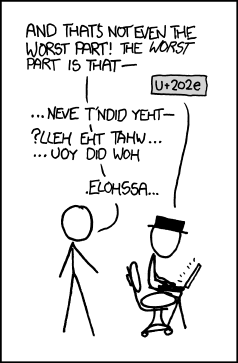
\includegraphics[height=0.65\textheight]{externalfig/rtl.png}\\
Collaborative editing can quickly become a textual rap battle fought with increasingly convoluted invocations of U+202a to U+202e (\href{https://xkcd.com/1137/}{xkcd.com/1137})
\end{frame}

%------------------------------------------------------------%

\begin{frame}{Session 4: Aim (Chapter 7.1 + 7.2)}
\pause - conditional coding (if-else)\\
\pause - repetitional coding (for-loops)\\
\pause afterwards, you should be able to:
\pause
\begin{itemize}[<+->]
\item make reasonable guesses about logical values by looking at code
\item write conditionally executed code using if/else
\item decide whether to use \rcode{if(cond) A else B} or \rcode{ifelse(cond, A, B)}
\item explain the concept of a loop
\item write simple for-loops
\end{itemize}
\end{frame}

%------------------------------------------------------------%

\begin{frame}[fragile]{Session 4: Recap}
\begin{itemize}[<+->]
\item \rcode{if(TRUE) message("Yo!") else message("Dude...")}
\item be careful with line breaks
\item \rcode{ifelse(c(T,T,F,T), 7, else 7.3)} for vectors
\item loops repeat a block of code with a different \rcode{i} each time
\item \rcode{for(i in 1:20) plot(df[,i], main=colnames(df)[i])}
\item for loops should not be called too often, as they are slow
\item instead: vectorize, use lapply, write C++ code
\end{itemize}
\end{frame}

%------------------------------------------------------------%

\begin{frame}{Session 4: Homework }
\begin{enumerate}[<+->]
  \item Exam task in Chapter 12
  \item Update your RefCard: mark all the items you learned about today
  \item Write down topics you want to learn (more) about in the optional session
  \item Do actual research, have fun!
\end{enumerate}
\onslide<+->
Please email me how much time you spent on each task and how solvable it was (did you need to look into my solutions?)
\end{frame}

%------------------------------------------------------------%
%------------------------------------------------------------%
\subsection{Session 5/4: Additional material}
%------------------------------------------------------------%
%------------------------------------------------------------%

\begin{frame}[fragile]{recap \alert{if else} I}
\begin{enumerate}
\item Create a new R file and write \rcode{x <- 3.14} into it.
\item Now  assign the absolute value of x to \rcode{y} by using conditional code execution (control structures).
\item \rcode{source} the complete document.
\item Test the result of y by setting \rcode{x <- -007} and running the document again.
\item BONUS: Make it also work for vectors like \rcode{x <- (-5):8} .
\end{enumerate}
\pause
\begin{knitrout}
\definecolor{shadecolor}{rgb}{0.961, 0.961, 0.961}\color{fgcolor}\begin{kframe}
\begin{alltt}
\hlstd{x} \hlkwb{<-} \hlopt{-}\hlnum{5}\hlopt{:}\hlnum{8}
\hlstd{y} \hlkwb{<-} \hlkwd{ifelse}\hlstd{(x}\hlopt{<}\hlnum{0}\hlstd{,} \hlopt{-}\hlstd{x, x)}
\hlstd{y}
\end{alltt}
\begin{verbatim}
##  [1] 5 4 3 2 1 0 1 2 3 4 5 6 7 8
\end{verbatim}
\end{kframe}
\end{knitrout}
\end{frame}

%------------------------------------------------------------%

\begin{frame}[fragile]{recap \alert{if else} II}
\begin{knitrout}
\definecolor{shadecolor}{rgb}{0.961, 0.961, 0.961}\color{fgcolor}\begin{kframe}
\begin{alltt}
\hlstd{(}  \hlkwd{requireNamespace}\hlstd{(}\hlstr{"some_package"}\hlstd{,} \hlkwc{quietly}\hlstd{=}\hlnum{TRUE}\hlstd{)  )}
\end{alltt}
\begin{verbatim}
## [1] FALSE
\end{verbatim}
\end{kframe}
\end{knitrout}
invisibly returns TRUE if it succeeds loading a package. The outer brackets are for printing in the slides.
\begin{enumerate}
\item Use it to conditionally install the package \href{https://cran.r-project.org/package=quantmod}{quantmod} (i.e. if it is not already available).
\end{enumerate}
\pause
\begin{knitrout}\small
\definecolor{shadecolor}{rgb}{0.961, 0.961, 0.961}\color{fgcolor}\begin{kframe}
\begin{alltt}
\hlkwa{if}\hlstd{(}\hlopt{!}\hlkwd{requireNamespace}\hlstd{(}\hlstr{"quantmod"}\hlstd{))} \hlkwd{install.packages}\hlstd{(}\hlstr{"quantmod"}\hlstd{)}
\end{alltt}


{\ttfamily\noindent\itshape\color{messagecolor}{\#\# Loading required namespace: quantmod}}\end{kframe}
\end{knitrout}
\end{frame}

%------------------------------------------------------------%
%------------------------------------------------------------%
\subsection{Feedback}
%------------------------------------------------------------%
%------------------------------------------------------------%

\begin{frame}{Feedback}
\center{
Please fill out the feedback form at\\[1em]
\href{https://goo.gl/jVgqge}{goo.gl/jVgqge}\\[1em]
(it only takes 2 minutes)\\[1em]
Thanks!\\[1em]
}
\end{frame}

%------------------------------------------------------------%
%------------------------------------------------------------%
\section{1. One-Session-Intro}
%------------------------------------------------------------%
%------------------------------------------------------------%

%------------------------------------------------------------%
%------------------------------------------------------------%
\subsection{Intro, objects, vectors}
%------------------------------------------------------------%
%------------------------------------------------------------%

\begin{frame}{\rcode{print("Hello world!")}}
\begin{itemize}[<+->]
\item Berry Boessenkool $\rightarrow$ berry-b@gmx.de
\item Geoecology @ Potsdam University \onslide<+-> - BSc\onslide<+->, MSc\onslide<+->, \textit{PhD (trying)}
\item R Fan\onslide<+->atic \onslide<+-> since 2010
\item Teaching: \href{https://rclickhandbuch.wordpress.com}{RclickHandbuch.wordpress.com} (German)
\item Programming: \href{https://github.com/brry}{github.com/brry/\texttt{extremeStat}}, \onslide<+->\href{https://cran.r-project.org/package=berryFunctions}{cran.r-project.org/package=\texttt{berryFunctions}}
%\item \alert{Jump to beta distribution \hyperlink{beta}{example lecture}}
\item These slides were originally based on a one week course held in 2013 for \href{http://www.cawa-project.net/story/300}{CaWa} with Mathias Seibert (GFZ) in Bishkek, Kyrgyzstan
\item \alert{If we're proceeding too fast, please interrupt me!}
\end{itemize}
\end{frame}

%------------------------------------------------------------%

\begin{frame}{Why programming?}
\pause
\begin{itemize}[<+->]
  \item Data analysis
  \item Plotting
  \onslide<+->  \vspace{-0.5em} ~~~~~~~~~ \textit{Excel could do that, but is lacking} \vspace{0.5em}
  \item Awesomeness
    \begin{itemize}
    \item efficiency
    \item flexibility
    \item automatization
    \item transparency, reproducibility
    \item complex statistical procedures
    \item \textcolor{ForestGreen}{job chance advantage}
    \end{itemize}
\end{itemize}
\onslide<+-> Why R? (and not matlab, python, java, html, C++, fortran)
\begin{itemize}[<+->]
  \item Open Source $\rightarrow$ free!
  \item Large community $\rightarrow$ stunning lots of methods!
  \item Interpreter language $\rightarrow$ no compilation, human readable code
  \item The standard for data analysis in many universities and industries
\end{itemize}
\end{frame}

%------------------------------------------------------------%

\begin{frame}{In the future, programming will save you time!}

\includegraphics[width=0.99\textwidth]{externalfig/xkcd3.PNG}\\
I find that when someone's taking time to do something right in the present, they're a perfectionist with no ability to prioritize, whereas when someone took time to do something right in the past, they're a master artisan of great foresight. (\href{https://xkcd.com/974/}{xkcd.com/974})\\
\end{frame}

%------------------------------------------------------------%

\begin{frame}{Get started in R}
\pause
\begin{exercise}{R is an awesome calculator}
In the console, calculate ~ 21+21 ~,~ 7*6 ~ and ~ $\frac{0,3}{4}*\sqrt{313600}$
\end{exercise}
\vspace{-1em}
\pause
\begin{knitrout}
\definecolor{shadecolor}{rgb}{0.961, 0.961, 0.961}\color{fgcolor}\begin{kframe}
\begin{alltt}
\hlnum{21}\hlopt{+}\hlnum{21} \hlstd{;} \hlnum{7}\hlopt{*}\hlnum{6} \hlstd{;} \hlnum{0.3}\hlopt{/}\hlnum{4}\hlopt{*}\hlkwd{sqrt}\hlstd{(}\hlnum{313600}\hlstd{)}
\end{alltt}
\end{kframe}
\end{knitrout}
\vspace{-1em}
\pause
\begin{itemize}[<+->]
  \item objects: assignment with ~ \rcode{$<-$} ~ Rstudio Keyboard shortcut:  \rcode{ALT} + \rcode{-}  \\
        \rcode{nstudents <- 15\\nstudents\\nstudents > 12}
  \item What's a good object name? \onslide<+-> $\rightarrow$ short, but explanatory,
        \onslide<+-> lowerCamelStandard\_or\_underscore are good naming conventions
  \item comments: \texttt{\textcolor[rgb]{0,0.392,0}{\# everything after a hashtag is not executed.}}
  \item scripts: Rstudio
\end{itemize}
\end{frame}

%------------------------------------------------------------%

\begin{frame}{Objects: vectors}
\begin{itemize}[<+->]
  \item To create a vector with values, use the syntax\\
  \rcode{values <- c(3, -11, 13, 5.94)} \texttt{\textcolor[rgb]{0,0.392,0}{\# \textbf{c}oncatenate, \textbf{c}ombine}}
  \item To obtain a subset (=indexing), use square brackets: \rcode{values[2]}
\end{itemize}
\onslide<+->
\begin{exercise}{Vector indexing}
\begin{enumerate}
  \item Create a vector with body sizes of people around you. You can also use the values 1.75, 1.76, 1.83, 1.84, 1.77, 1.76, 1.77, 1.66, 1.86, 1.76. Assign it to an object with a useful name (\rcode{YourObject} is not one!).
  \item What does \rcode{3:6} create? What does \rcode{YourObject[3:6]} do?
  \item What does \rcode{YourObject[-4]} do?
  \item BONUS (for fast people): Analyze the descriptive statistics: \rcode{mean(YourObject), median, min, max, range, quantile}
  \item BONUS 2: Help your peers - there's no reason to be bored ;-)
\end{enumerate}
\end{exercise}
\end{frame}

%------------------------------------------------------------%

\begin{frame}[fragile]{Vector task solutions}
\begin{knitrout}
\definecolor{shadecolor}{rgb}{0.961, 0.961, 0.961}\color{fgcolor}\begin{kframe}
\begin{alltt}
\hlstd{size} \hlkwb{<-} \hlkwd{c}\hlstd{(}\hlnum{1.75}\hlstd{,} \hlnum{1.76}\hlstd{,} \hlnum{1.83}\hlstd{,} \hlnum{1.84}\hlstd{,} \hlnum{1.77}\hlstd{,} \hlnum{1.76}\hlstd{,}
          \hlnum{1.77}\hlstd{,} \hlnum{1.66}\hlstd{,} \hlnum{1.86}\hlstd{,} \hlnum{1.76}\hlstd{)}
\hlnum{3}\hlopt{:}\hlnum{6} \hlcom{# A vector with consecutive integers}
\hlstd{size[}\hlnum{3}\hlopt{:}\hlnum{6}\hlstd{]} \hlcom{# Select the corresponding elements of a vector}
\hlstd{size[}\hlopt{-}\hlnum{4}\hlstd{]} \hlcom{# Select all but the fourth value}
\end{alltt}
\end{kframe}
\end{knitrout}
\begin{knitrout}\scriptsize
\definecolor{shadecolor}{rgb}{0.961, 0.961, 0.961}\color{fgcolor}\begin{kframe}
\begin{alltt}
\hlkwd{c}\hlstd{(}\hlkwd{mean}\hlstd{(size),} \hlkwd{median}\hlstd{(size),} \hlkwd{min}\hlstd{(size),} \hlkwd{max}\hlstd{(size));} \hlkwd{range}\hlstd{(size);} \hlkwd{quantile}\hlstd{(size)}
\end{alltt}
\begin{verbatim}
## [1] 1.776 1.765 1.660 1.860
## [1] 1.66 1.86
##    0%   25%   50%   75%  100% 
## 1.660 1.760 1.765 1.815 1.860
\end{verbatim}
\end{kframe}
\end{knitrout}

\rcode{mean} and \rcode{median} are similar, hinting at a symmetric data distribution\\
\rcode{range} returns a composite of \rcode{min}imum and \rcode{max}imum\\
\rcode{quantile} returns \href{http://lmgtfy.com/?q=quantile}{quantiles} (now that is surprising...)
\end{frame}

%------------------------------------------------------------%
%------------------------------------------------------------%
\subsection{Files, data.frames}
%------------------------------------------------------------%
%------------------------------------------------------------%

\begin{frame}{Reading files}

\onslide<+->
\begin{exercise}{Reading files}
Copy the file \datalink{treesize.txt} and tell R where to look for it with:\\
\rcode{setwd("C:/path/to/input")} \texttt{\textcolor[rgb]{0,0.392,0}{ \# change back- to forwardslashes}}\\
  \onslide<+-> Read the file into R with the command \rcode{read.table}.\\
  \onslide<+-> If R tells you "no such file" exists, check the output of \rcode{dir()}.\\
  \onslide<+-> Use the documentation to find out the correct settings of the arguments:\\
  \onslide<+-> \rcode{help(read.table)}, \rcode{?read.table}, or press F1.\\
  \onslide<+-> \rcode{str(YourObject)} must yield the column data types: \texttt{num, num, factor}. \\
  \onslide<+-> You need to set the argument \texttt{header}.
  \end{exercise}
\end{frame}

%------------------------------------------------------------%

\begin{frame}[fragile]{Solution to exercise \arabic{exercisecount}: Reading files}
\begin{knitrout}
\definecolor{shadecolor}{rgb}{0.961, 0.961, 0.961}\color{fgcolor}\begin{kframe}
\begin{alltt}
\hlstd{treesize} \hlkwb{<-} \hlkwd{read.table}\hlstd{(}\hlkwc{file}\hlstd{=}\hlstr{"treesize.txt"}\hlstd{,} \hlkwc{header}\hlstd{=}\hlnum{TRUE}\hlstd{)}
\end{alltt}
\end{kframe}
\end{knitrout}
\end{frame}

%------------------------------------------------------------%

\begin{frame}{Objects: data.frames}
\vspace{-0.5em}
\begin{itemize}[<+->]
  \item For tables with different data types (numbers, characters, categories, integers), R has the object type data.frame: \\\rcode{data.frame(count=c(2,6,5), type=c("a","k","k"))}
  \item \rcode{read.table} also returns a data.frame
  \item If we have the object \rcode{df}, we can subset with \rcode{df[rows,columns]}
  \item \rcode{df[1,2:4]; df[2, ]; df[ ,"name"]; df\$name}
  \item Logical values: \rcode{vect[c(TRUE,TRUE,FALSE,FALSE,TRUE,FALSE)]}
\end{itemize}
\onslide<+->
\begin{exercise}{Data.frame indexing}
  From the dataset \rcode{treesize} from the previous exercise, obtain:
  \begin{enumerate}
  \item The first 5 values in column 2
  \item The maximum "Height" (the maximum of the values in that column)
  \item For each entry: is the measurement equal to (\rcode{==}) A?
  \item BONUS 1: The height entries for trees older than 23.5 years
  \item BONUS 2: All rows, excluding rows 3, 7,8,9,...,20
  \end{enumerate}
\end{exercise}
\end{frame}

%------------------------------------------------------------%

\begin{frame}[fragile]{Solution to exercise \arabic{exercisecount}: subsetting data.frames I}
\begin{knitrout}\scriptsize
\definecolor{shadecolor}{rgb}{0.961, 0.961, 0.961}\color{fgcolor}\begin{kframe}
\begin{alltt}
\hlstd{treesize[}\hlnum{1}\hlopt{:}\hlnum{5}\hlstd{,} \hlnum{2}\hlstd{]}
\end{alltt}
\begin{verbatim}
## [1] 32.7 26.0 27.9 35.4 26.4
\end{verbatim}
\begin{alltt}
\hlkwd{max}\hlstd{(treesize}\hlopt{$}\hlstd{height)  ;}   \hlkwd{max}\hlstd{(treesize[ ,}\hlstr{"age"}\hlstd{])}
\end{alltt}
\begin{verbatim}
## [1] 40.1
## [1] 24.8
\end{verbatim}
\begin{alltt}
\hlstd{treesize}\hlopt{$}\hlstd{measurement}\hlopt{==}\hlstr{"A"}
\end{alltt}
\begin{verbatim}
##   [1]  TRUE  TRUE  TRUE  TRUE FALSE FALSE  TRUE  TRUE  TRUE  TRUE  TRUE FALSE
##  [13]  TRUE  TRUE  TRUE FALSE  TRUE FALSE FALSE FALSE  TRUE FALSE  TRUE  TRUE
##  [25]  TRUE FALSE  TRUE FALSE FALSE FALSE FALSE  TRUE  TRUE FALSE FALSE FALSE
##  [37] FALSE  TRUE FALSE  TRUE FALSE FALSE  TRUE  TRUE  TRUE FALSE FALSE FALSE
##  [49]  TRUE FALSE  TRUE  TRUE  TRUE  TRUE FALSE FALSE  TRUE  TRUE FALSE FALSE
##  [61]  TRUE  TRUE FALSE FALSE  TRUE FALSE  TRUE FALSE  TRUE FALSE FALSE FALSE
##  [73] FALSE FALSE FALSE FALSE  TRUE FALSE  TRUE FALSE FALSE  TRUE  TRUE  TRUE
##  [85] FALSE FALSE FALSE FALSE  TRUE FALSE  TRUE  TRUE FALSE  TRUE  TRUE FALSE
##  [97]  TRUE FALSE  TRUE  TRUE
\end{verbatim}
\end{kframe}
\end{knitrout}
\end{frame}

%------------------------------------------------------------%

\begin{frame}[fragile]{Solution to exercise \arabic{exercisecount}: subsetting data.frames II}
\begin{knitrout}\scriptsize
\definecolor{shadecolor}{rgb}{0.961, 0.961, 0.961}\color{fgcolor}\begin{kframe}
\begin{verbatim}
##  [1] 32.7 38.4 40.1 34.0 32.3 32.6 34.4 23.2 34.6
## [10] 35.9
\end{verbatim}
\end{kframe}
\end{knitrout}
\begin{knitrout}\scriptsize
\definecolor{shadecolor}{rgb}{0.961, 0.961, 0.961}\color{fgcolor}\begin{kframe}
\begin{alltt}
\hlstd{treesize[} \hlopt{-}\hlkwd{c}\hlstd{(}\hlnum{3}\hlstd{,}\hlnum{7}\hlopt{:}\hlnum{20}\hlstd{) , ]}

\hlcom{#}
\end{alltt}
\end{kframe}
\end{knitrout}
\vspace{-3em}
\begin{knitrout}\scriptsize
\definecolor{shadecolor}{rgb}{0.961, 0.961, 0.961}\color{fgcolor}\begin{kframe}
\begin{verbatim}
##     age height measurement
## 1  24.4   32.7           A
## 2  13.6   26.0           A
## 4  21.2   35.4           A
## 5  19.8   26.4           B
## 6   7.7    7.2           B
## 21  5.1    7.2           A
## 22 15.6   17.7           B
## 23 19.4   29.2           A
## 24  7.8   10.2           A
## 25  5.7   11.1           A
## 26 19.6   17.5           B
## 27 12.8   20.1           A
## ...
\end{verbatim}
\end{kframe}
\end{knitrout}
\end{frame}

%------------------------------------------------------------%
%------------------------------------------------------------%
\subsection{Plotting}
%------------------------------------------------------------%
%------------------------------------------------------------%

\begin{frame}[fragile]{Plotting I}
General code for scatterplots: \rcode{plot(x, y, ...)}
\pause
\begin{knitrout}
\definecolor{shadecolor}{rgb}{0.961, 0.961, 0.961}\color{fgcolor}\begin{kframe}
\begin{alltt}
\hlkwd{plot}\hlstd{(}\hlkwc{x}\hlstd{=Indometh}\hlopt{$}\hlstd{time,} \hlkwc{y}\hlstd{=Indometh}\hlopt{$}\hlstd{conc,}
     \hlkwc{col}\hlstd{=}\hlstr{"orange"}\hlstd{,} \hlkwc{pch}\hlstd{=}\hlnum{16}\hlstd{,} \hlkwc{main}\hlstd{=}\hlstr{"Awesome Graph!"}\hlstd{)}
\end{alltt}
\end{kframe}

{\centering \includegraphics[width=\textwidth]{./fig/plot_indo1-1} 

}



\end{knitrout}
\end{frame}

%------------------------------------------------------------%

\begin{frame}[fragile]{Plotting I}
General code for scatterplots: \rcode{plot(x, y, ...)}
\begin{knitrout}
\definecolor{shadecolor}{rgb}{0.961, 0.961, 0.961}\color{fgcolor}\begin{kframe}
\begin{alltt}
\hlkwd{points}\hlstd{(}\hlnum{4}\hlstd{,} \hlnum{1.5}\hlstd{,} \hlkwc{pch}\hlstd{=}\hlnum{22}\hlstd{,} \hlkwc{bg}\hlstd{=}\hlstr{"yellow"}\hlstd{,} \hlkwc{cex}\hlstd{=}\hlnum{4}\hlstd{,} \hlkwc{col}\hlstd{=}\hlstr{"red"}\hlstd{)}
\hlcom{# PointCHaracter, BackGround, Character EXpansion}
\end{alltt}
\end{kframe}

{\centering \includegraphics[width=\textwidth]{./fig/plot_indo2-1} 

}



\end{knitrout}
\end{frame}

%------------------------------------------------------------%

\begin{frame}[fragile]{Plotting I}
General code for scatterplots: \rcode{plot(x, y, ...)}
\begin{knitrout}
\definecolor{shadecolor}{rgb}{0.961, 0.961, 0.961}\color{fgcolor}\begin{kframe}
\begin{alltt}
\hlkwd{lines}\hlstd{(}\hlkwc{x}\hlstd{=}\hlkwd{c}\hlstd{(}\hlnum{2}\hlstd{,}\hlnum{5}\hlstd{,}\hlnum{6}\hlstd{,}\hlnum{7}\hlstd{),} \hlkwc{y}\hlstd{=}\hlkwd{c}\hlstd{(}\hlnum{1}\hlstd{,}\hlnum{2.3}\hlstd{,}\hlopt{-}\hlnum{3}\hlstd{,}\hlnum{1}\hlstd{),}
      \hlkwc{col}\hlstd{=}\hlnum{4}\hlstd{,} \hlkwc{type}\hlstd{=}\hlstr{"b"}\hlstd{,} \hlkwc{lwd}\hlstd{=}\hlnum{5}\hlstd{)}
\end{alltt}
\end{kframe}

{\centering \includegraphics[width=\textwidth]{./fig/plot_indo3-1} 

}



\end{knitrout}
\end{frame}

%------------------------------------------------------------%

\begin{frame}[fragile]{Plotting II: Our treesize dataset}
\vspace{-1em}
%Code to read the file:
\begin{knitrout}\small
\definecolor{shadecolor}{rgb}{0.961, 0.961, 0.961}\color{fgcolor}\begin{kframe}
\begin{alltt}
\hlstd{treesize} \hlkwb{<-} \hlkwd{read.table}\hlstd{(}\hlkwc{file}\hlstd{=}\hlstr{"data/treesize.txt"}\hlstd{,} \hlkwc{header}\hlstd{=}\hlnum{TRUE}\hlstd{)}
\end{alltt}
\end{kframe}
\end{knitrout}
\pause
%General code for scatterplots:
\begin{knitrout}
\definecolor{shadecolor}{rgb}{0.961, 0.961, 0.961}\color{fgcolor}\begin{kframe}
\begin{alltt}
\hlkwd{plot}\hlstd{(}\hlkwc{x}\hlstd{=xvalues,} \hlkwc{y}\hlstd{=y_values,} \hlkwc{xlab}\hlstd{=}\hlstr{"nice axis label"}\hlstd{,}
     \hlkwc{main}\hlstd{=}\hlstr{"graph title"}\hlstd{,} \hlkwc{las}\hlstd{=}\hlnum{1}\hlstd{)}
\end{alltt}
\end{kframe}
\end{knitrout}
\pause
\begin{exercise}{Scatterplots, sample distribution graphs}
\begin{enumerate}%[<+->]
  \item Plot tree height over age.
  \item Add labels to the plot.
  \item Change the point character (\rcode{pch}) and color (\rcode{col}).
  \item BONUS 1: Use a vector for colors, e.g. treesize\$measurement
  \item BONUS 2: Compare the histogram (\rcode{hist}) of the heights with the \rcode{boxplot} and \rcode{quantile(x, probs=c(0.1, 0.8))}.
\end{enumerate}
\end{exercise}
\end{frame}

%------------------------------------------------------------%

\begin{frame}[fragile]{Solution for exercise \arabic{exercisecount}: Scatterplots}
\begin{knitrout}\footnotesize
\definecolor{shadecolor}{rgb}{0.961, 0.961, 0.961}\color{fgcolor}\begin{kframe}
\begin{alltt}
\hlstd{treesize} \hlkwb{<-} \hlkwd{read.table}\hlstd{(}\hlkwc{file}\hlstd{=}\hlstr{"data/treesize.txt"}\hlstd{,} \hlkwc{header}\hlstd{=}\hlnum{TRUE}\hlstd{)}

\hlkwd{plot}\hlstd{(treesize}\hlopt{$}\hlstd{age, treesize}\hlopt{$}\hlstd{height)}
\hlkwd{plot}\hlstd{(treesize}\hlopt{$}\hlstd{age, treesize}\hlopt{$}\hlstd{height,} \hlkwc{las}\hlstd{=}\hlnum{1}\hlstd{,} \hlkwc{ylab}\hlstd{=}\hlstr{"Tree height [m]"}\hlstd{,}
     \hlkwc{xlab}\hlstd{=}\hlstr{"Tree age [years]"}\hlstd{,} \hlkwc{col}\hlstd{=treesize}\hlopt{$}\hlstd{measurement,}
     \hlkwc{main}\hlstd{=}\hlstr{"Older trees are larger"}\hlstd{,} \hlkwc{pch}\hlstd{=}\hlnum{3}\hlstd{)}
\hlkwd{quantile}\hlstd{(treesize}\hlopt{$}\hlstd{height,} \hlkwc{probs}\hlstd{=}\hlkwd{c}\hlstd{(}\hlnum{0.1}\hlstd{,} \hlnum{0.8}\hlstd{))}
\end{alltt}
\begin{verbatim}
##   10%   80% 
##  8.93 32.36
\end{verbatim}
\end{kframe}
\end{knitrout}
\end{frame}

%------------------------------------------------------------%

\begin{frame}[fragile]{Solution for exercise \arabic{exercisecount}: Scatterplot}
\includegraphics[width=\linewidth]{fig/solscatplot-2.pdf}
\end{frame}

%------------------------------------------------------------%

\begin{frame}[fragile]{Solution for exercise \arabic{exercisecount}: Histogram}
\begin{knitrout}
\definecolor{shadecolor}{rgb}{0.961, 0.961, 0.961}\color{fgcolor}\begin{kframe}
\begin{alltt}
\hlkwd{hist}\hlstd{(treesize}\hlopt{$}\hlstd{height,} \hlkwc{col}\hlstd{=}\hlnum{6}\hlstd{,} \hlkwc{breaks}\hlstd{=}\hlnum{20}\hlstd{,} \hlkwc{las}\hlstd{=}\hlnum{1}\hlstd{)}
\end{alltt}
\end{kframe}

{\centering \includegraphics[width=\textwidth]{./fig/solscathist-1} 

}



\end{knitrout}
\end{frame}

%------------------------------------------------------------%

\begin{frame}[fragile]{Solution for exercise \arabic{exercisecount}: Boxplot}
\begin{knitrout}
\definecolor{shadecolor}{rgb}{0.961, 0.961, 0.961}\color{fgcolor}\begin{kframe}
\begin{alltt}
\hlkwd{boxplot}\hlstd{(treesize}\hlopt{$}\hlstd{height,} \hlkwc{col}\hlstd{=}\hlnum{5}\hlstd{,} \hlkwc{horizontal}\hlstd{=}\hlnum{TRUE}\hlstd{,} \hlkwc{notch}\hlstd{=}\hlnum{TRUE}\hlstd{)}
\end{alltt}
\end{kframe}

{\centering \includegraphics[width=\textwidth]{./fig/solscatbox-1} 

}



\end{knitrout}
\end{frame}

%------------------------------------------------------------%

\begin{frame}[fragile]{commonly needed \rcode{plot} arguments}
\begin{knitrout}
\definecolor{shadecolor}{rgb}{0.961, 0.961, 0.961}\color{fgcolor}\begin{kframe}
\begin{alltt}
\hlkwd{plot}\hlstd{(x, y,} \hlcom{# point coordinates}
\hlkwc{col}\hlstd{=}\hlstr{"lightblue"}\hlstd{,} \hlcom{# point color}
\hlkwc{pch}\hlstd{=}\hlnum{0}\hlstd{,} \hlcom{# point character (symbol)}
\hlkwc{xlab}\hlstd{=}\hlstr{"My label  [km]"}\hlstd{,} \hlkwc{ylab}\hlstd{=}\hlstr{""}\hlstd{,} \hlcom{# axis labels}
\hlkwc{main}\hlstd{=}\hlstr{"Graph title"}\hlstd{,} \hlcom{# title}
\hlkwc{cex}\hlstd{=}\hlnum{1.8}\hlstd{,} \hlcom{# character expansion (symbol size)}
\hlkwc{type}\hlstd{=}\hlstr{"l"}\hlstd{,} \hlcom{# draw lines instead of points}
\hlkwc{lwd}\hlstd{=}\hlnum{3}\hlstd{,} \hlcom{# line width (thickness of lines)}
\hlkwc{las}\hlstd{=}\hlnum{1}\hlstd{,} \hlcom{# label axis type (axis numbers upright)}
\hlkwc{xaxt}\hlstd{=}\hlstr{"n"} \hlcom{# axis type (none to suppress axis)}
\hlstd{)}
\end{alltt}
\end{kframe}
\end{knitrout}
\end{frame}

%------------------------------------------------------------%
%------------------------------------------------------------%
\subsection{Packages, regression}
%------------------------------------------------------------%
%------------------------------------------------------------%

\begin{frame}[fragile]{R Packages}
\begin{itemize}[<+->]
\item Many people write code for specific tasks and publish it on CRAN, the Comprehensive R Archive Network
\item Packages for a range of topics: \href{http://cran.r-project.org/web/views/}{cran.r-project.org/web/views}
\item All $>$10'500 available packages: \href{http://cran.r-project.org/web/packages/}{cran.r-project.org/web/packages}
\item \rcode{install.packages("ggplot2")} to download and install.\\ 
      \footnotesize (only needs to be executed once, works on user level, no admin rights required)\\
      You can do this in Rstudio \normalsize
\item \rcode{library("ggplot2")} to load it \\
      \footnotesize (needed in every new R session) Put this in the script for reproducibility \normalsize
\item Better to use the \rcode{package::function} syntax
\item Regularly run \rcode{update.packages()} or use the Rstudio button
\item Rarely needed: \rcode{remove.packages("packagename")}
\end{itemize}
\end{frame}

%------------------------------------------------------------%

\begin{frame}[fragile]{Packages and linear regression}
\begin{exercise}{Packages, linear regression}
\begin{enumerate}
  \item Install and load the package \rcode{berryFunctions}
  \item How can we pass the treesize data to \rcode{?linReg} with a formula?
  \item Describe the resulting graph (height vs age).
  \item Look into the source code of \rcode{linReg}. What is actually the backbone for the calculation of the function?
  \item Feed the data into \rcode{lm}, assign the output to an object (useful name!).
  \item Briefly explain the \rcode{summary} of the linear model.
\end{enumerate}
\end{exercise}
\end{frame}

%------------------------------------------------------------%

\begin{frame}[fragile]{Solution for exercise \arabic{exercisecount}: Linear regression}
\vspace{-1em}
\begin{knitrout}\footnotesize
\definecolor{shadecolor}{rgb}{0.961, 0.961, 0.961}\color{fgcolor}\begin{kframe}
\begin{alltt}
\hlkwd{library}\hlstd{(}\hlstr{"berryFunctions"}\hlstd{)}
\hlkwd{linReg}\hlstd{(height}\hlopt{~}\hlstd{age,} \hlkwc{data}\hlstd{=treesize)}
\hlstd{linReg}
\hlkwd{browseURL}\hlstd{(}\hlstr{"https://github.com/brry/berryFunctions"}\hlstd{)}
\hlcom{# go to R/linReg.R  -  working horse: lm}
\hlstd{linear_model} \hlkwb{<-} \hlkwd{lm}\hlstd{(height}\hlopt{~}\hlstd{age,} \hlkwc{data}\hlstd{=treesize)}
\hlkwd{summary}\hlstd{(linear_model)}
\end{alltt}
\end{kframe}
\end{knitrout}
\vspace{-1em}
\small
\href{http://blog.yhathq.com/posts/r-lm-summary.html}{blog.yhathq.com/posts/r-lm-summary.html}\\
\href{http://stats.stackexchange.com/questions/5135/interpretation-of-rs-lm-output}{stats.stackexchange.com/questions/5135/interpretation-of-rs-lm-output}
\normalsize
\begin{knitrout}
\definecolor{shadecolor}{rgb}{0.961, 0.961, 0.961}\color{fgcolor}

{\centering \includegraphics[width=\textwidth]{./fig/sollinreg2-1} 

}



\end{knitrout}
\end{frame}

%' %------------------------------------------------------------%
%' %------------------------------------------------------------%
%' \subsection{Packages, normality test}
%' %------------------------------------------------------------%
%' %------------------------------------------------------------%
%'
%' \begin{frame}[fragile]{Test for normality of a distribution}
%' \pause
%' \begin{itemize}[<+->]
%'   \item If a population is normally distributed, it is described by only two parameters: the mean (position) and the sd (width, dispersion) of the bell shaped curve.
%'   \item This is an important assumption for many classical statistical methods.
%'   \item Whether a dataset is normally distributed can be checked with a histogram (visually effective, but the class limits are subjective), with qqplots (I don't find them very intuitive), or with statistical tests.
%' \item
%' <<normaltest, eval=F>>=
%' data <- rnorm(1000, mean=97, sd=8.9)
%' shapiro.test(data)
%' ks.test(data, "pnorm", mean(data), sd(data))
%' # if p > 0.05: accept the Null-hypothesis
%' # that data are normally distributed.
%' @
%' \end{itemize}
%' \end{frame}
%'
%' %------------------------------------------------------------%
%'
%' \begin{frame}{Packages, normality test}
%' \begin{itemize}[<+->]
%'   \item Many people write code for specific tasks and publish it on CRAN, the Comprehensive R Archive Network
%'   \item \rcode{install.packages("ggplot2")} to download and install\\ (only needs to be executed once, requires internet connection)
%'   \item \rcode{library("ggplot2")} to load it (in every new R session)
%' \end{itemize}
%' \onslide<+->
%' \begin{exercise}{Packages, normality test}
%' \begin{enumerate}
%'   \item Install and load the package \rcode{nortest}
%'   \item Open the package documentation (see \rcode{?help})
%'   \item Run and compare several tests for normality: \rcode{shapiro.test}, \rcode{ks.test}\\
%'         Lilliefors (Kolmogorov-Smirnov), Anderson-Darling, Cramer-von Mises, Pearson chi-square, Shapiro-Francia
%'   \item BONUS: With random numbers generated from a normal distribution (\rcode{rnorm}),
%'         study the sensitivity / stability of each of the tests (What do you obtain in repeated application?).
%' \end{enumerate}
%' \end{exercise}
%' \end{frame}
%'
%' %------------------------------------------------------------%
%'
%' \begin{frame}[fragile]{Solution for exercise \arabic{exercisecount}: normality test}
%' \vspace{-1em}
%' <<solnortest, eval=TRUE, size="footnotesize">>=
%' if(!requireNamespace("nortest")) install.packages("nortest")
%' library(nortest)          # with Lilliefors-correction!
%' help(package="nortest")
%' d <- treesize$height[treesize$measurement=="A"]
%' lillie.test(d)  # Lilliefors (Kolmogorov-Smirnov) test for normality
%' ad.test(d)      # Anderson-Darling test for normality
%' @
%' \end{frame}
%'
%' %------------------------------------------------------------%
%'
%' \begin{frame}[fragile]{Solution for exercise \arabic{exercisecount}: normality test}
%' <<solnortest2, eval=TRUE, size="tiny">>=
%' cvm.test(d)     # Cramer-von Mises test for normality
%' pearson.test(d) # Pearson chi-square test for normality
%' sf.test(d)      # Shapiro-Francia test for normality
%' @
%' \end{frame}

%------------------------------------------------------------%

\begin{frame}{Time to put all of this into practice}
\begin{exercise}{Reading files, subsetting, comparison}%1
\begin{enumerate}
  \item Start a new session of R. Read in the tree size data.
  \item Check that everything is read correctly with \rcode{str}.
  \item \rcode{which} rows of the data.frame have measurement equal to (\rcode{==}) B?
  \item Plot the linear regression for measurement method B, then add the points and regression line for A in a different color and shape.
  \item BONUS 1: use \rcode{boxplot} with a formula (\rcode{height\textasciitilde measurement})
               for an automatic boxplot comparison with median difference notches.
 \item BONUS 2: Visually compare the effect of Girth and Height on Volume in the dataset \rcode{trees}. Here's one idea (of many possible): Plot with two panels below each other (\rcode{par(mfrow=c(2,1)}), with the linear regression plots (\rcode{berryFunctions::linReg}) for each variable. Make it look nice with the graphical \rcode{par}ameters \texttt{mar} and \texttt{mgp}, as well as by specifying some of the linReg arguments.
\end{enumerate}
\end{exercise}
\end{frame}

%------------------------------------------------------------%

\begin{frame}[fragile]{Solution for exercise \arabic{exercisecount}: Reading files, subsetting}
\begin{knitrout}\footnotesize
\definecolor{shadecolor}{rgb}{0.961, 0.961, 0.961}\color{fgcolor}\begin{kframe}
\begin{alltt}
\hlkwd{setwd}\hlstd{(}\hlstr{"D:/my/path"}\hlstd{)}
\hlstd{treesize} \hlkwb{<-} \hlkwd{read.table}\hlstd{(}\hlkwc{file}\hlstd{=}\hlstr{"data/treesize.txt"}\hlstd{,} \hlkwc{header}\hlstd{=}\hlnum{TRUE}\hlstd{)}
\hlkwd{str}\hlstd{(treesize)}
\end{alltt}
\end{kframe}
\end{knitrout}
\vspace{-1em}
\begin{knitrout}\footnotesize
\definecolor{shadecolor}{rgb}{0.961, 0.961, 0.961}\color{fgcolor}\begin{kframe}
\begin{alltt}
\hlkwd{which}\hlstd{(treesize}\hlopt{$}\hlstd{measurement}\hlopt{==}\hlstr{"B"}\hlstd{)}
\end{alltt}
\begin{verbatim}
##  [1]  5  6 12 16 18 19 20 22 26 28 29 30 31 34 35
## [16] 36 37 39 41 42 46 47 48 50 55 56 59 60 63 64
## [31] 66 68 70 71 72 73 74 75 76 78 80 81 85 86 87
## [46] 88 90 93 96 98
\end{verbatim}
\begin{alltt}
\hlstd{treeA} \hlkwb{<-} \hlstd{treesize[treesize}\hlopt{$}\hlstd{measurement}\hlopt{==}\hlstr{"A"}\hlstd{, ]}
\hlstd{treeB} \hlkwb{<-} \hlstd{treesize[treesize}\hlopt{$}\hlstd{measurement}\hlopt{==}\hlstr{"B"}\hlstd{, ]}
\hlkwd{library}\hlstd{(}\hlstr{"berryFunctions"}\hlstd{)}
\hlkwd{linReg}\hlstd{(height}\hlopt{~}\hlstd{age,} \hlkwc{data}\hlstd{=treeA,} \hlkwc{pos1}\hlstd{=}\hlstr{"topleft"}\hlstd{)}
\hlkwd{linReg}\hlstd{(height}\hlopt{~}\hlstd{age,} \hlkwc{data}\hlstd{=treeB,} \hlkwc{add}\hlstd{=T,} \hlkwc{col}\hlstd{=}\hlnum{4}\hlstd{,}
       \hlkwc{pos1}\hlstd{=}\hlstr{"bottomright"}\hlstd{,} \hlkwc{inset}\hlstd{=}\hlnum{0.05}\hlstd{)}
\hlkwd{points}\hlstd{(height}\hlopt{~}\hlstd{age,} \hlkwc{data}\hlstd{=treeB,} \hlkwc{pch}\hlstd{=}\hlnum{3}\hlstd{,} \hlkwc{col}\hlstd{=}\hlnum{4}\hlstd{)}
\end{alltt}
\end{kframe}
\end{knitrout}
\end{frame}

%------------------------------------------------------------%

\begin{frame}[fragile]{Solution for exercise \arabic{exercisecount}: Plotting, linear Regression}
\includegraphics[width=.99\textwidth]{fig/introsol2-1.pdf}
\end{frame}

%------------------------------------------------------------%

\begin{frame}[fragile]{Solution for exercise \arabic{exercisecount}.BONUS 1}
\begin{knitrout}
\definecolor{shadecolor}{rgb}{0.961, 0.961, 0.961}\color{fgcolor}\begin{kframe}
\begin{alltt}
\hlkwd{boxplot}\hlstd{(height}\hlopt{~}\hlstd{measurement,} \hlkwc{data}\hlstd{=treesize,}
        \hlkwc{col}\hlstd{=}\hlkwd{c}\hlstd{(}\hlstr{"blue"}\hlstd{,}\hlstr{"orange"}\hlstd{),} \hlkwc{notch}\hlstd{=}\hlnum{TRUE}\hlstd{)}
\end{alltt}
\end{kframe}

{\centering \includegraphics[width=\textwidth]{./fig/introsol3-1} 

}



\end{knitrout}
\end{frame}

%------------------------------------------------------------%

\begin{frame}[fragile]{Solution for exercise \arabic{exercisecount}.BONUS 2}
\begin{knitrout}\scriptsize
\definecolor{shadecolor}{rgb}{0.961, 0.961, 0.961}\color{fgcolor}\begin{kframe}
\begin{alltt}
\hlkwd{par}\hlstd{(}\hlkwc{mfrow}\hlstd{=}\hlkwd{c}\hlstd{(}\hlnum{2}\hlstd{,}\hlnum{1}\hlstd{),} \hlkwc{mar}\hlstd{=}\hlkwd{c}\hlstd{(}\hlnum{3}\hlstd{,}\hlnum{3}\hlstd{,}\hlnum{1.5}\hlstd{,}\hlnum{0.5}\hlstd{),} \hlkwc{mgp}\hlstd{=}\hlkwd{c}\hlstd{(}\hlnum{1.9}\hlstd{,}\hlnum{0.7}\hlstd{,}\hlnum{0}\hlstd{),} \hlkwc{las}\hlstd{=}\hlnum{1}\hlstd{)}
\hlkwd{linReg}\hlstd{(Volume}\hlopt{~}\hlstd{Height,} \hlkwc{data}\hlstd{=trees,} \hlkwc{col}\hlstd{=}\hlstr{"blue"}\hlstd{,} \hlkwc{pos1}\hlstd{=}\hlstr{"topleft"}\hlstd{)}
\hlkwd{linReg}\hlstd{(Volume}\hlopt{~}\hlstd{Girth,} \hlkwc{data}\hlstd{=trees,} \hlkwc{col}\hlstd{=}\hlstr{"forestgreen"}\hlstd{,} \hlkwc{pos1}\hlstd{=}\hlstr{"topleft"}\hlstd{)}
\end{alltt}
\end{kframe}

{\centering \includegraphics[width=.95\textwidth]{./fig/introsol4-1} 

}



\end{knitrout}
\end{frame}

%------------------------------------------------------------%
%------------------------------------------------------------%
\section{2. Getting started: Background, GUI and first steps}
%------------------------------------------------------------%
%------------------------------------------------------------%

%------------------------------------------------------------%
%------------------------------------------------------------%
\subsection{Background information}
%------------------------------------------------------------%
%------------------------------------------------------------%

\begin{frame}{R - What and Why?}
\pause
\begin{itemize}%[<+->]
\item R is a standard environment for statistical computing
\item and an object-oriented programming language.
\item It is developed and maintained by the R development core team
\item and has thousands of add-on packages written by the community.
\item There are mailing lists where users (\& developers) help users
\item and blogs to communicate analysis and coding to the public.
\item R allows complex data analysis of big data sets with current methods
\item and the creation of advanced professional (even interactive) graphics.
\item Coding and programming forces you to keep track of your work
\item and allows you to efficiently customize and automatize your analysis.
\item R is very versatile: you can write your own functions and packages,
\item implement new methods and make them available to everyone.
\item Being capable of programming helps finding a job
\item and the best part: \textcolor{green}{R is open source and free!}
\end{itemize}
\pause
\small \href{http://fantasyfootballanalytics.net/2014/01/why-r-is-better-than-excel.html}{fantasyfootballanalytics.net/2014/01/why-r-is-better-than-excel.html}
\href{http://thegrantlab.org/bio3d/tutorials/79-static-content/85-why-use-r}{thegrantlab.org/bio3d/tutorials/79-static-content/85-why-use-r}
\end{frame}

%------------------------------------------------------------%

\begin{frame}{interpreter language - no compilation}
\pause
\centering
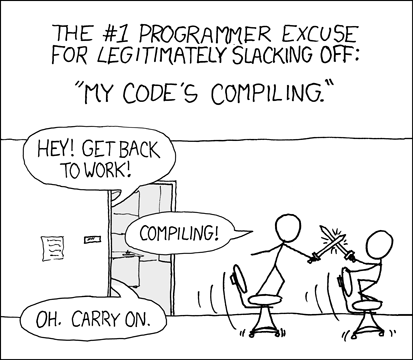
\includegraphics[height=0.65\textheight]{externalfig/compiling.png}\\
\href{https://xkcd.com/303/}{xkcd.com/303}
\end{frame}

%------------------------------------------------------------%

% \begin{frame}{R is growing increasingly popular}
%   \begin{figure}[h]
%   	\begin{center}
% 		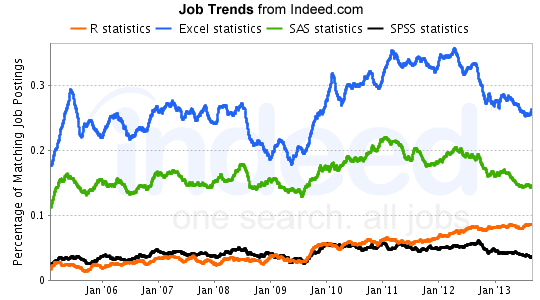
\includegraphics[width=.8\linewidth]{./externalfig/jobgraph.png}
% 		\caption{\href{http://www.indeed.com/jobanalytics/}{www.indeed.com/jobanalytics}}
% 		\label{fig:r-jobs}
%     \end{center}
% 	\end{figure}
% \end{frame}

%------------------------------------------------------------%

\begin{frame}{Where to get R}
%\pause
\begin{itemize}%[<+->]
  \item base R itself: \href{https://cloud.r-project.org/}{r-project.org}.\\
        \href{https://cran.r-project.org/bin/linux/ubuntu/README.html}{Official} and \href{https://www.r-bloggers.com/how-to-install-r-on-linux-ubuntu-16-04-xenial-xerus/}{helpful} hints for Linux Ubuntu users.
  \item Use an Editor to work with script files:
  \item \href{https://www.rstudio.com/products/rstudio/\#Desktop}{R-Studio} (widely spread, easy to use)
  \item \href{http://sourceforge.net/projects/tinn-r/}{Tinn-R} (only for Windows OS, flexible window arrangement).\\
         Needs some initial tweaking, see \href{https://rclickhandbuch.wordpress.com/install-r/tinn-r_english}{Berry's TinnR Page} % pdf cannot be completed without this percent sign
\end{itemize}
\label{installR}
\end{frame}

%------------------------------------------------------------%
%------------------------------------------------------------%
\subsection{Graphical user interfaces}
%------------------------------------------------------------%
%------------------------------------------------------------%

% \begin{frame}{Working with R: Basic R GUI and Command line}
%   \begin{figure}[h]
%   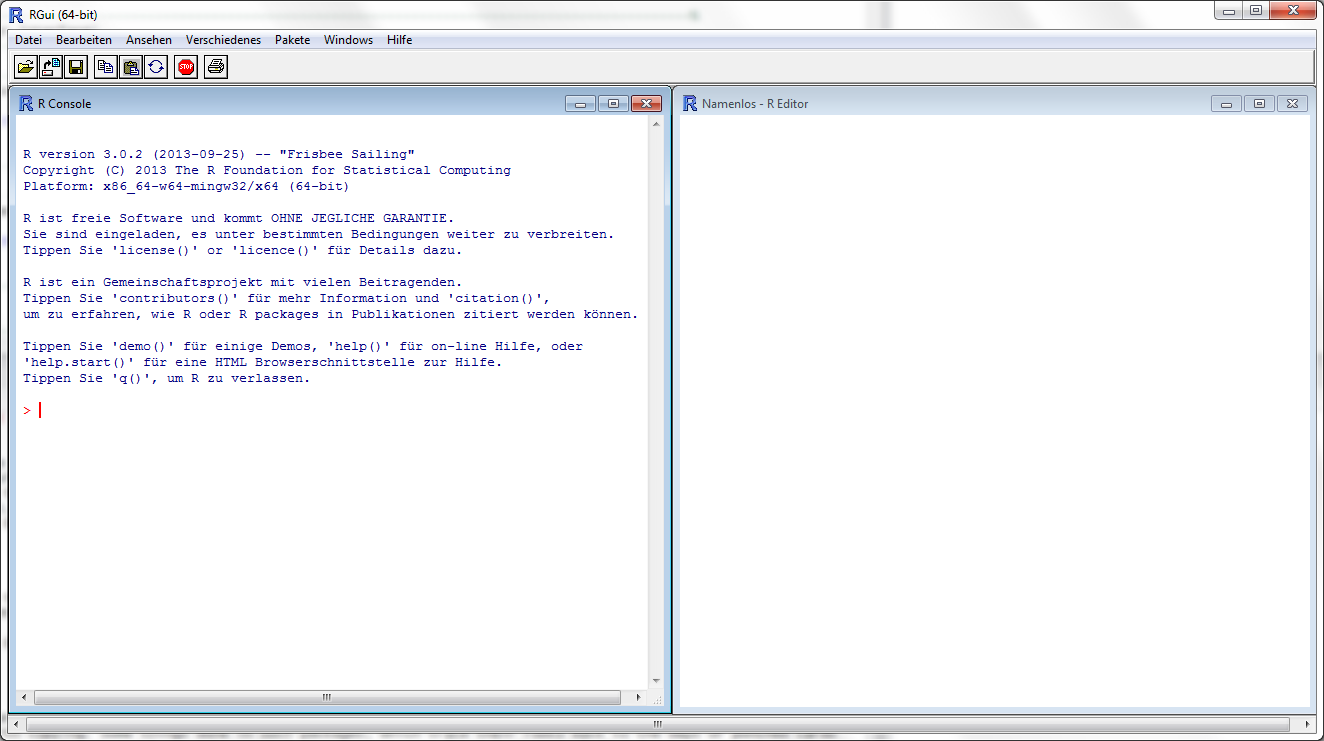
\includegraphics[width=\textwidth]{./externalfig/rgui.png}
%   \end{figure}
% \end{frame}

%------------------------------------------------------------%

\begin{frame}{RStudio}
  \begin{figure}
  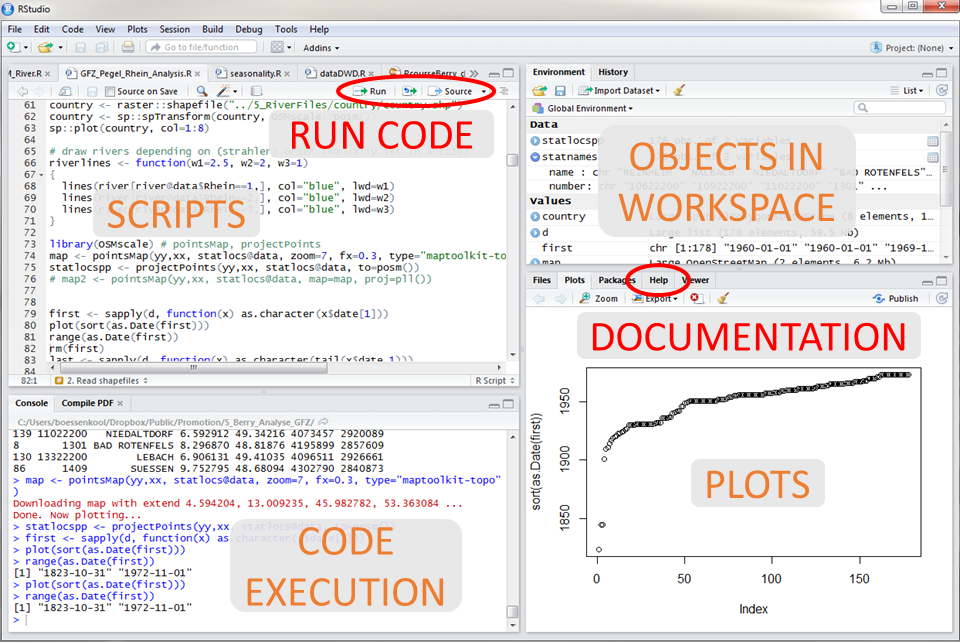
\includegraphics[width=0.95\textwidth]{./externalfig/Rstudio.png}
  \end{figure}
\end{frame}

%------------------------------------------------------------%

\begin{frame}{RStudio configuration}
\href{https://support.rstudio.com/hc/en-us/articles/200711853-Keyboard-Shortcuts}{keyboard shortcuts} (ALT+SHIFT+K)\\[1em]
\pause
Recommended settings for reproducible research under\\
\alert{Tools - Global Options - General}\\
\textbf{ON}: Restore previously open source documents at startup\\
\textbf{OFF}: Restore .Rdata into workspace at startup\\
Save workspace to .RData on exit: \textbf{NEVER}\\[0.5em]
% \textbf{OFF}: Always save history (even when not saving .RData)\\[0.5em]
\pause
\textit{Instead use \rcode{save(object, file="object.Rdata")} after long computations.
You can load them later with \rcode{load("object.Rdata")}.}\\[1em]
\pause
\alert{Tools - Global Options - Code - Display}\\
\textbf{ON}: Show margin (Margin column:80) ~~~~\textit{People \textbf{hate} horizontal scrolling!}\\[0.5em]
\alert{Tools - Global Options - Code - Saving}\\
Line ending conversion: \textbf{Windows (CR/LF)}
\end{frame}

%------------------------------------------------------------%

\begin{frame}[fragile]{Tinn R}
  \begin{figure}[h]
    \begin{center}
    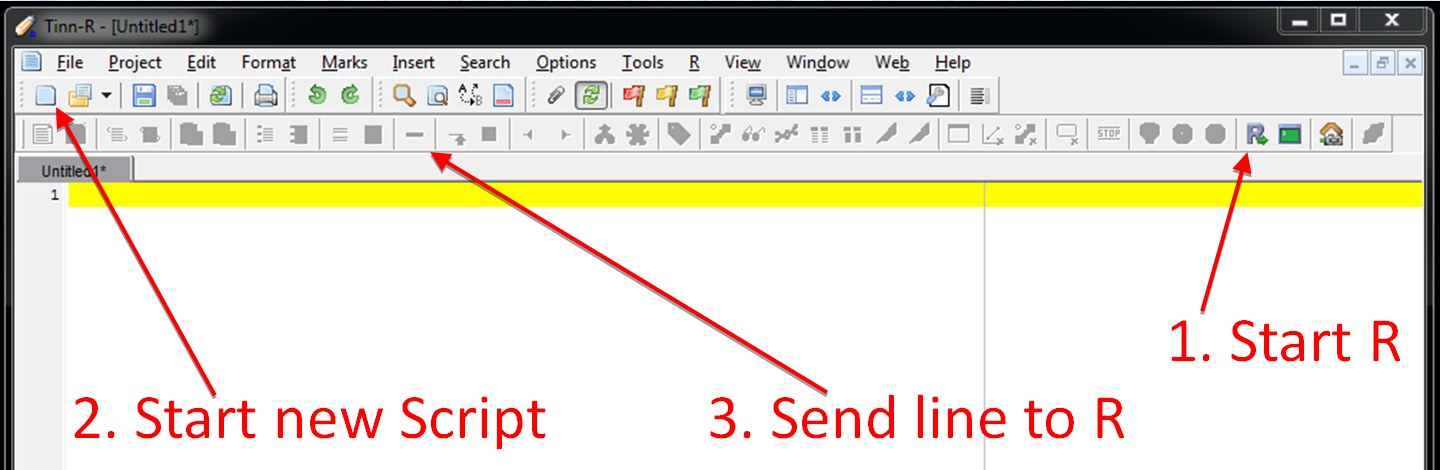
\includegraphics[width=.8\linewidth]{./externalfig/TinnR_gui.png}
		\caption{screenshot Tinn-R}
		\label{fig:how to start R from Tinn-R}
    \end{center}
	\end{figure}
\begin{knitrout}\scriptsize
\definecolor{shadecolor}{rgb}{0.961, 0.961, 0.961}\color{fgcolor}\begin{kframe}
\begin{alltt}
\hlcom{# enable sending of blocks up to the next blank line:}
\hlstd{.trPaths} \hlkwb{<-} \hlkwd{paste}\hlstd{(}\hlkwd{Sys.getenv}\hlstd{(}\hlstr{'LOCALAPPDATA'}\hlstd{),}
\hlstr{'\textbackslash{}\textbackslash{}Temp\textbackslash{}\textbackslash{}Tinn-R'}\hlstd{,} \hlkwd{c}\hlstd{(}\hlstr{''}\hlstd{,} \hlstr{'search.txt'}\hlstd{,} \hlstr{'objects.txt'}\hlstd{,}
\hlstr{'file.r'}\hlstd{,} \hlstr{'selection.r'}\hlstd{,} \hlstr{'block.r'}\hlstd{,}\hlstr{'lines.r'}\hlstd{),}\hlkwc{sep}\hlstd{=}\hlstr{'\textbackslash{}\textbackslash{}'}\hlstd{)}
\hlcom{# write this in  C:/Program Files/R/R-3.2.2/etc/Rprofile.site}
\end{alltt}
\end{kframe}
\end{knitrout}
\end{frame}

%------------------------------------------------------------%
%------------------------------------------------------------%
\subsection{Getting help}
%------------------------------------------------------------%
%------------------------------------------------------------%

\begin{frame}[fragile]{Getting help: Inside R}
  R-Help
\begin{knitrout}
\definecolor{shadecolor}{rgb}{0.961, 0.961, 0.961}\color{fgcolor}\begin{kframe}
\begin{alltt}
\hlkwd{help}\hlstd{(}\hlstr{"apply"}\hlstd{)} \hlcom{# get help for the function}
\hlopt{?}\hlstd{apply} \hlcom{# The same. saves typing effort.}
\hlcom{# Press F1 while the cursor is at a command.}

\hlkwd{apropos}\hlstd{(}\hlstr{"apply"}\hlstd{)}
\hlkwd{help.search}\hlstd{(}\hlstr{"apply"}\hlstd{)}
\hlopt{??}\hlstd{apply}

\hlkwd{help.start}\hlstd{()} \hlcom{# html help Manuals, Material, search engine}
\end{alltt}
\end{kframe}
\end{knitrout}
\end{frame}

%------------------------------------------------------------%

\begin{frame}[fragile]{Getting help: Outside R}
\pause
\begin{itemize}[<+->]
  \item \href{https://cran.r-project.org/manuals.html}{R-Manuals} for introduction to the language
  \item R Wiki: \href{http://rwiki.sciviews.org/}{rwiki.sciviews.org}
  \item Ref Cards:
    \href{https://www.rstudio.com/wp-content/uploads/2016/09/r-cheat-sheet-1.pdf}{base} and
    \href{https://www.rstudio.com/wp-content/uploads/2016/02/advancedR.pdf}{advanced} cheatsheets from
    \href{https://www.rstudio.com/resources/cheatsheets/}{Rstudio},\\
    RefCards originally by Tom Short from
    \href{https://github.com/jonasstein/R-Reference-Card/raw/master/R-refcard.pdf}{Stein} (recommended),
    \href{https://cran.r-project.org/doc/contrib/Baggott-refcard-v2.pdf}{Baggot},
    \href{http://www.u.arizona.edu/~kuchi/Courses/MAT167/Files/R-refcard.pdf}{Tanbakuchi},
    \href{http://atrey.karlin.mff.cuni.cz/~morf/vyuka/pas/materialy/R-refcard.pdf}{cuni} or
    \href{http://statmaster.sdu.dk/bent/courses/ST501-2011/Rcard.pdf}{Joergensen}
	\item \href{www.rseek.org}{rseek.org} for R related internet search
  \item \href{www.StackOverflow.com}{StackOverflow} for programming questions <-- \alert{main resource}
  \item \href{www.CrossValidated.com}{CrossValidated} for statistical questions
	\item Mailing lists: ask other experienced users for help
	\begin{itemize}
  \item \href{http://www.r-project.org/mail.html}{R-help mailing list}
  \item \href{http://r.789695.n4.nabble.com/}{Nabble}: Forum-like view of the r-help mailing list
  \item ONLY post on mailing lists when all other options are exploited and you are sure there's no answer out there. FIRST read the \href{http://www.r-project.org/posting-guide.html}{posting guide}.
\end{itemize}
\end{itemize}
\label{refcards}
\end{frame}

%------------------------------------------------------------%

% \begin{frame}[fragile]{R related internet search}
%   \begin{figure}[h]
%     \begin{center}
% 		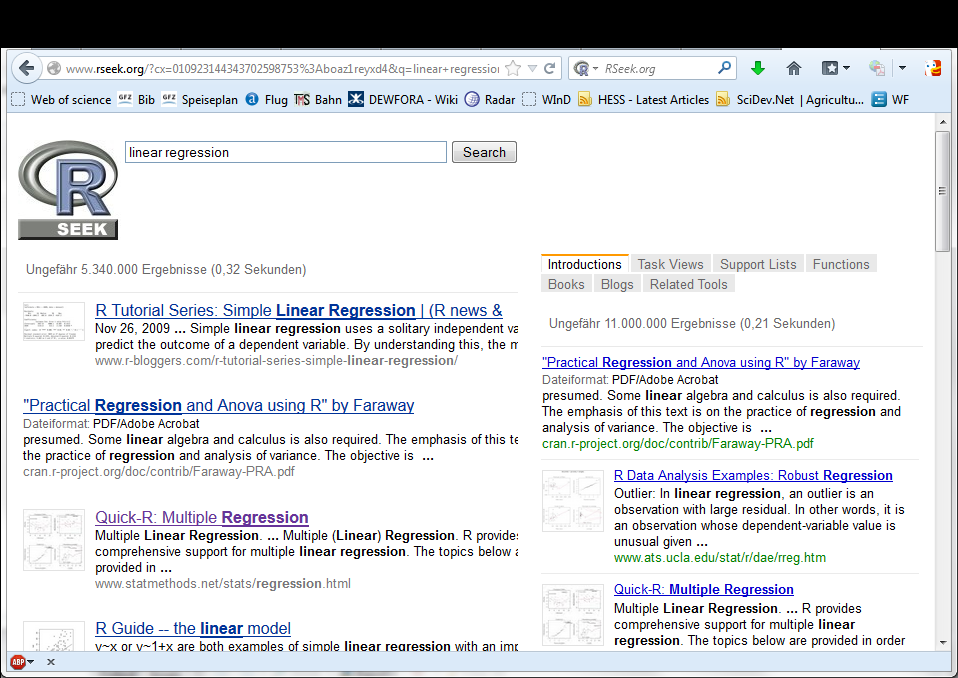
\includegraphics[width=.75\linewidth]{./externalfig/rseek.png}
% 		\caption{\href{http://www.rseek.org}{www.rseek.org}}
% 		\label{fig:rseek}
%     \end{center}
% 	\end{figure}
% \end{frame}

%------------------------------------------------------------%

\begin{frame}[fragile]{Good References, books }%(\datalink{books.zip})}
\begin{itemize}[<+->]
\item J. Adler (2010): R in a Nutshell
\item U. Ligges (2008): Programmieren mit R (German)
\item M. Crawley (2007): The R-book
\item H. Wickham (2014) \href{http://adv-r.had.co.nz}{Advanced R}
\item H. Wickham (2015) \href{http://r-pkgs.had.co.nz}{R Packages}
\item domain specific: \href{http://www.crcpress.com/browse/series/crctherser}{Chapman and Hall R Series}
\item Many more listed at \href{https://github.com/RomanTsegelskyi/rbooks}{github.com/RomanTsegelskyi/rbooks}
\item Review list at \href{https://web.archive.org/web/20130619094650/http://ecotope.org/blogs/page/R-Book-Review.aspx}{ecotope.org, through the wayback machine}
\end{itemize}
\onslide<+-> Tutorials:
\begin{itemize}[<+->]
\item \href{http://RclickHandbuch.wordpress.com}{RclickHandbuch.wordpress.com} (German)
\item \href{https://www.edx.org/course/introduction-r-programming-microsoft-dat204x-0#!}{Microsoft + Datacamp} (best course I know of, with login, but free)
\item \href{http://tryr.codeschool.com/levels/1/challenges/1}{tryR.codeschool.com} (interactive)
\item \href{http://stat545-ubc.github.io/topics.html}{STAT 545}
\end{itemize}
\label{books}
\end{frame}

%------------------------------------------------------------%
%------------------------------------------------------------%
\subsection{R syntax}
%------------------------------------------------------------%
%------------------------------------------------------------%

\begin{frame}[fragile]{get started, comments}
Please start R via the editor you like.\\[\baselineskip]
Comments start with a hash key \# %\textbf{\#}\\

\begin{knitrout}
\definecolor{shadecolor}{rgb}{0.961, 0.961, 0.961}\color{fgcolor}\begin{kframe}
\begin{alltt}
\hlnum{17}\hlopt{-}\hlnum{42} \hlcom{# This is a comment, thus not executed}
\end{alltt}
\begin{verbatim}
## [1] -25
\end{verbatim}
\end{kframe}
\end{knitrout}
\end{frame}

%------------------------------------------------------------%

\begin{frame}{Please calculate the following tasks}
\begin{exercise}{Basic operators} %ex1
\begin{enumerate}
  \item 4 * 9\\
  \item 2 + 4,8 (International decimal sign: ".")\\
  \item $3^2$\\
  \item $\frac{\pi}{2}$\\
  \item sinus of 15$\,^{\circ}$. Must be 0.26. Remember: $ radians = degrees*\frac{\pi}{180\,^{\circ} } $\\ % $ for math\\
  \item $\sqrt{81}$  (square root)\\
  \item $|-12|$ (absolute value)\\
  \item log(100) (--$>$ should return 2, as $10^2$ = 100 )\\
  \item 5! (factorial)\\
  \item $e^3$ (exponential function)\\
  \item Bonus: How is 3.91 * $10^{ -3}$ written in scientific notation?
\end{enumerate}
\end{exercise}
\end{frame}

%------------------------------------------------------------%

\begin{frame}[fragile]{Solution for exercise \arabic{exercisecount}.1-8: Basic operators}
\begin{knitrout}
\definecolor{shadecolor}{rgb}{0.961, 0.961, 0.961}\color{fgcolor}\begin{kframe}
\begin{alltt}
\hlnum{4}\hlopt{*}\hlnum{9} \hlcom{# this is our first calculation with a comment}
\hlnum{2} \hlopt{+} \hlnum{4.8}
\hlnum{3}\hlopt{^}\hlnum{2}
\hlstd{pi}\hlopt{/}\hlnum{2}
\hlkwd{sin}\hlstd{(}\hlnum{15}\hlopt{*}\hlstd{pi}\hlopt{/}\hlnum{180}\hlstd{)}
\hlopt{?}\hlstd{sqrt} \hlcom{# get the offline help about the function sqrt}
\hlkwd{sqrt}\hlstd{(}\hlnum{81}\hlstd{)} \hlcom{# square root}
\hlkwd{abs}\hlstd{(}\hlopt{-}\hlnum{12}\hlstd{)} \hlcom{# absolute value}
\hlkwd{log}\hlstd{(}\hlnum{100}\hlstd{)}
\hlkwd{help}\hlstd{(log)} \hlcom{# natural logarithm}
\hlkwd{log10}\hlstd{(}\hlnum{100}\hlstd{)} \hlcom{# log base 10}
\hlkwd{log}\hlstd{(}\hlnum{100}\hlstd{,} \hlkwc{base}\hlstd{=}\hlnum{10}\hlstd{)} \hlcom{# another way}
\end{alltt}
\end{kframe}
\end{knitrout}
\end{frame}

%------------------------------------------------------------%

\begin{frame}[fragile]{Solution for exercise \arabic{exercisecount}.9-11: Basic operators}
\begin{knitrout}
\definecolor{shadecolor}{rgb}{0.961, 0.961, 0.961}\color{fgcolor}\begin{kframe}
\begin{alltt}
\hlkwd{factorial}\hlstd{(}\hlnum{5}\hlstd{)}
\hlstd{e}\hlopt{^}\hlnum{3} \hlcom{# does not work}
\hlopt{??}\hlstd{exponential}
\hlkwd{exp}\hlstd{(}\hlnum{3}\hlstd{)} \hlcom{# exponential function}
\hlkwd{exp}\hlstd{(}\hlnum{1}\hlstd{)} \hlcom{# the value of e}
\hlnum{3.91} \hlopt{*} \hlnum{10}\hlopt{^-}\hlnum{3}
\hlnum{3.91e-3} \hlcom{# no spaces possible in scientific notation}
\hlkwd{help.start}\hlstd{()} \hlcom{# offline search, manuals, etc}
\end{alltt}
\end{kframe}
\end{knitrout}
\end{frame}

%------------------------------------------------------------%
%------------------------------------------------------------%
\subsection{Source code of R commands}
%------------------------------------------------------------%
%------------------------------------------------------------%

\begin{frame}
Source code: \href{https://github.com/wch/r-source/tree/trunk/src/library}{github.com/wch/r-source/src/library}/base (or stats, utils, ...)\\
CRAN packages source code: \href{https://github.com/cran}{github.com/cran}\\
HTML Documentation: \href{https://www.rdocumentation.org/packages/berryFunctions/versions/1.12.3/topics/colPoints}{www.rdocumentation.org}\\[0.5em]

\href{http://stackoverflow.com/questions/19226816/how-can-i-view-the-source-code-for-a-function}{excellent post}

ncol - .Primitive("dim") - NROW
head.matrix
https://github.com/wch/r-source/blob/trunk/src/library/utils/R/head.R
https://github.com/wch/r-source/blob/trunk/src/library/base/R/matrix.R

\end{frame}

%------------------------------------------------------------%
%------------------------------------------------------------%
\section{3. Objects}
%------------------------------------------------------------%
%------------------------------------------------------------%

%------------------------------------------------------------%
%------------------------------------------------------------%
\subsection{Assignments}
%------------------------------------------------------------%
%------------------------------------------------------------%

\begin{frame}[fragile]{Assignment:  Create an object with data in the workspace I}
\begin{knitrout}
\definecolor{shadecolor}{rgb}{0.961, 0.961, 0.961}\color{fgcolor}\begin{kframe}
\begin{alltt}
\hlstd{a} \hlkwb{<-} \hlnum{15.4}
\end{alltt}
\end{kframe}
\end{knitrout}
\onslide<2->
\begin{knitrout}
\definecolor{shadecolor}{rgb}{0.961, 0.961, 0.961}\color{fgcolor}\begin{kframe}
\begin{alltt}
\hlstd{a}
\end{alltt}
\begin{verbatim}
## [1] 15.4
\end{verbatim}
\end{kframe}
\end{knitrout}
\onslide<3->
\begin{knitrout}
\definecolor{shadecolor}{rgb}{0.961, 0.961, 0.961}\color{fgcolor}\begin{kframe}
\begin{alltt}
\hlstd{a} \hlopt{>} \hlnum{2} \hlcom{# is a bigger than 2?  --> logical value (boolean)}
\end{alltt}
\begin{verbatim}
## [1] TRUE
\end{verbatim}
\end{kframe}
\end{knitrout}
\onslide<4->
\begin{knitrout}
\definecolor{shadecolor}{rgb}{0.961, 0.961, 0.961}\color{fgcolor}\begin{kframe}
\begin{alltt}
\hlstd{A} \hlcom{# not an existing object (R is case sensitive)}
\end{alltt}


{\ttfamily\noindent\bfseries\color{errorcolor}{\#\# Error in eval(expr, envir, enclos): object 'A' not found}}\end{kframe}
\end{knitrout}
\end{frame}

%------------------------------------------------------------%

\begin{frame}[fragile]{Assignment:  Create an object with data in the workspace II}
Don't assign to existing objects or functions like \rcode{mean, c, T, data, sin}; \onslide<+-> Later on, you will hardly be able to distinguish what object (original or custom) you are referring to.\\ % \onslide<+-> (Advanced users: your own funtions will be lost if you overwrite them).\\
\onslide<+->
As R is Case SeNsitivE, \rcode{Data} would be OK, but it's not useful. Use object names that are short, but still meaningful.\\
\onslide<+->
One convention is lowerCamel:\\
\rcode{dailyRainBerlin} is short and readable through capital letters
\onslide<+->
\begin{knitrout}
\definecolor{shadecolor}{rgb}{0.961, 0.961, 0.961}\color{fgcolor}\begin{kframe}
\begin{alltt}
\hlcom{# Rstudio: press 'ALT' + '-'  for   " <- "}
\end{alltt}
\end{kframe}
\end{knitrout}
\onslide<+->
Don't use \rcode{=} for assignments. R users usually prefer " <- ", (\href{http://google-styleguide.googlecode.com/svn/trunk/Rguide.xml}{style guide}) and "=" is only allowed on the top level.\\ \onslide<+->
\rcode{median(x <- 1:10)} also creates the object in \rcode{globalenv()}, while \rcode{median(x=1:10)} does not.
Used in \rcode{NCOL}, for example.\\ 
\onslide<+->
\footnotesize{
\href{http://blog.revolutionanalytics.com/2008/12/use-equals-or-arrow-for-assignment.html}{http://blog.revolutionanalytics.com/2008/12/use-equals-or-arrow-for-assignment.html}
\href{https://csgillespie.wordpress.com/2010/11/16/assignment-operators-in-r-vs/}{https://csgillespie.wordpress.com/2010/11/16/assignment-operators-in-r-vs/}}
\end{frame}

%------------------------------------------------------------%
%------------------------------------------------------------%
\subsection{Vectors, indexing}
%------------------------------------------------------------%
%------------------------------------------------------------%

\begin{frame}[fragile]{Vectors I}

In R, Vectors are not geometric constructs, but an ordered set of values.\\
\onslide<+->
Create a vector with \rcode{c} (stands for Combine or Concatenate), separating each entry with a comma:
\onslide<+->
\begin{knitrout}
\definecolor{shadecolor}{rgb}{0.961, 0.961, 0.961}\color{fgcolor}\begin{kframe}
\begin{alltt}
\hlstd{b} \hlkwb{<-} \hlkwd{c}\hlstd{(}\hlnum{3}\hlstd{,} \hlnum{7}\hlstd{,} \hlopt{-}\hlnum{2.5}\hlstd{,} \hlnum{11}\hlstd{,} \hlnum{3.8}\hlstd{,} \hlnum{9}\hlstd{)}
\end{alltt}
\end{kframe}
\end{knitrout}
\onslide<+->
spaces make code easier to read:
\begin{knitrout}
\definecolor{shadecolor}{rgb}{0.961, 0.961, 0.961}\color{fgcolor}\begin{kframe}
\begin{alltt}
\hlstd{b}\hlkwb{<-}\hlkwd{c}\hlstd{(}\hlnum{3}\hlstd{,}\hlnum{7}\hlstd{,}\hlopt{-}\hlnum{2.5}\hlstd{,}\hlnum{11}\hlstd{,}\hlnum{3.8}\hlstd{,}\hlnum{9}\hlstd{)}
\hlstd{b} \hlkwb{<-} \hlkwd{c}\hlstd{(}\hlnum{3}\hlstd{,} \hlnum{7}\hlstd{,} \hlopt{-}\hlnum{2.5}\hlstd{,} \hlnum{11}\hlstd{,} \hlnum{3.8}\hlstd{,} \hlnum{9}\hlstd{)}
\end{alltt}
\end{kframe}
\end{knitrout}
\onslide<+->
\begin{knitrout}
\definecolor{shadecolor}{rgb}{0.961, 0.961, 0.961}\color{fgcolor}\begin{kframe}
\begin{alltt}
\hlkwd{print}\hlstd{(b)} \hlcom{# or just write   b}
\end{alltt}
\begin{verbatim}
## [1]  3.0  7.0 -2.5 11.0  3.8  9.0
\end{verbatim}
\end{kframe}
\end{knitrout}
\end{frame}

%------------------------------------------------------------%

\begin{frame}[fragile]{Vectors II: Other ways to generate vectors}
\pause
\begin{knitrout}
\definecolor{shadecolor}{rgb}{0.961, 0.961, 0.961}\color{fgcolor}\begin{kframe}
\begin{alltt}
\hlnum{1}\hlopt{:}\hlnum{5}  \hlcom{# integer numbers  from : to}
\end{alltt}
\begin{verbatim}
## [1] 1 2 3 4 5
\end{verbatim}
\end{kframe}
\end{knitrout}
\onslide<3->
\begin{knitrout}
\definecolor{shadecolor}{rgb}{0.961, 0.961, 0.961}\color{fgcolor}\begin{kframe}
\begin{alltt}
\hlkwd{rep}\hlstd{(}\hlnum{1}\hlopt{:}\hlnum{4}\hlstd{,} \hlkwc{times}\hlstd{=}\hlnum{3}\hlstd{)} \hlcom{# repeat entries several times}
\end{alltt}
\begin{verbatim}
##  [1] 1 2 3 4 1 2 3 4 1 2 3 4
\end{verbatim}
\end{kframe}
\end{knitrout}
\onslide<4->
\begin{knitrout}
\definecolor{shadecolor}{rgb}{0.961, 0.961, 0.961}\color{fgcolor}\begin{kframe}
\begin{alltt}
\hlstd{v} \hlkwb{<-} \hlkwd{rep}\hlstd{(}\hlnum{1}\hlopt{:}\hlnum{3}\hlstd{,} \hlkwc{each}\hlstd{=}\hlnum{3}\hlstd{,} \hlkwc{times}\hlstd{=}\hlnum{2}\hlstd{)}
\hlstd{v}
\end{alltt}
\begin{verbatim}
##  [1] 1 1 1 2 2 2 3 3 3 1 1 1 2 2 2 3 3 3
\end{verbatim}
\end{kframe}
\end{knitrout}
\end{frame}

%------------------------------------------------------------%

\begin{frame}[fragile]{Vectors III: Yet other ways to generate vectors}
\pause
\begin{knitrout}
\definecolor{shadecolor}{rgb}{0.961, 0.961, 0.961}\color{fgcolor}\begin{kframe}
\begin{alltt}
\hlkwd{seq}\hlstd{(}\hlkwc{from}\hlstd{=}\hlnum{5}\hlstd{,} \hlkwc{to}\hlstd{=}\hlopt{-}\hlnum{1}\hlstd{,} \hlkwc{by}\hlstd{=}\hlopt{-}\hlnum{0.5}\hlstd{)} \hlcom{# Sequence}
\hlcom{# by must be negative for descending sequences}
\end{alltt}
\begin{verbatim}
##  [1]  5.0  4.5  4.0  3.5  3.0  2.5  2.0  1.5  1.0
## [10]  0.5  0.0 -0.5 -1.0
\end{verbatim}
\end{kframe}
\end{knitrout}
\onslide<3->
\begin{knitrout}
\definecolor{shadecolor}{rgb}{0.961, 0.961, 0.961}\color{fgcolor}\begin{kframe}
\begin{alltt}
\hlkwd{seq}\hlstd{(}\hlnum{1.32}\hlstd{,} \hlnum{6.1}\hlstd{,} \hlkwc{length.out}\hlstd{=}\hlnum{15}\hlstd{)} \hlcom{# 15 elements}
\end{alltt}
\begin{verbatim}
##  [1] 1.320000 1.661429 2.002857 2.344286 2.685714
##  [6] 3.027143 3.368571 3.710000 4.051429 4.392857
## [11] 4.734286 5.075714 5.417143 5.758571 6.100000
\end{verbatim}
\end{kframe}
\end{knitrout}
\onslide<4->
\begin{knitrout}
\definecolor{shadecolor}{rgb}{0.961, 0.961, 0.961}\color{fgcolor}\begin{kframe}
\begin{alltt}
\hlkwd{seq}\hlstd{(}\hlnum{1.32}\hlstd{,} \hlnum{6.1}\hlstd{,} \hlkwc{len}\hlstd{=}\hlnum{15}\hlstd{)} \hlcom{# abbreviate argument names}
\hlopt{?}\hlstd{seq} \hlcom{# read more about it...}
\end{alltt}
\end{kframe}
\end{knitrout}
\end{frame}

%------------------------------------------------------------%
%------------------------------------------------------------%
% \subsection{Indexing}
%------------------------------------------------------------%
%------------------------------------------------------------%

\begin{frame}[fragile]{Indexing on vectors (subsets) I: square brackets}
\begin{knitrout}
\definecolor{shadecolor}{rgb}{0.961, 0.961, 0.961}\color{fgcolor}\begin{kframe}
\begin{alltt}
\hlstd{b} \hlcom{# remember b?}
\end{alltt}
\begin{verbatim}
## [1]  3.0  7.0 -2.5 11.0  3.8  9.0
\end{verbatim}
\begin{alltt}
\hlstd{b[}\hlnum{1}\hlstd{]} \hlcom{# first element}
\end{alltt}
\begin{verbatim}
## [1] 3
\end{verbatim}
\end{kframe}
\end{knitrout}
\onslide<2->
\begin{knitrout}
\definecolor{shadecolor}{rgb}{0.961, 0.961, 0.961}\color{fgcolor}\begin{kframe}
\begin{alltt}
\hlstd{b[}\hlnum{2}\hlopt{:}\hlnum{4}\hlstd{]} \hlcom{# several elements}
\end{alltt}
\begin{verbatim}
## [1]  7.0 -2.5 11.0
\end{verbatim}
\begin{alltt}
\hlstd{b[} \hlkwd{c}\hlstd{(}\hlnum{2}\hlstd{,}\hlnum{5}\hlstd{,}\hlnum{1}\hlstd{,}\hlnum{6}\hlstd{,}\hlnum{1}\hlstd{) ]} \hlcom{# flexible}
\end{alltt}
\begin{verbatim}
## [1] 7.0 3.8 3.0 9.0 3.0
\end{verbatim}
\end{kframe}
\end{knitrout}
\end{frame}

%------------------------------------------------------------%

\begin{frame}[fragile]{Indexing on vectors (subsets) II}
\begin{knitrout}
\definecolor{shadecolor}{rgb}{0.961, 0.961, 0.961}\color{fgcolor}\begin{kframe}
\begin{alltt}
\hlstd{b}
\end{alltt}
\begin{verbatim}
## [1]  3.0  7.0 -2.5 11.0  3.8  9.0
\end{verbatim}
\begin{alltt}
\hlstd{b[}\hlopt{-}\hlnum{2}\hlstd{]} \hlcom{# all but the second element}
\end{alltt}
\begin{verbatim}
## [1]  3.0 -2.5 11.0  3.8  9.0
\end{verbatim}
\end{kframe}
\end{knitrout}
\onslide<2->
\begin{knitrout}
\definecolor{shadecolor}{rgb}{0.961, 0.961, 0.961}\color{fgcolor}\begin{kframe}
\begin{alltt}
\hlstd{a} \hlkwb{<-} \hlkwd{seq}\hlstd{(}\hlkwc{from}\hlstd{=}\hlnum{1}\hlstd{,} \hlkwc{to}\hlstd{=}\hlnum{100}\hlstd{,} \hlkwc{by}\hlstd{=}\hlnum{0.1}\hlstd{)}

\hlkwd{head}\hlstd{(a)} \hlcom{# only first 6 elements (or rows)}
\end{alltt}
\begin{verbatim}
## [1] 1.0 1.1 1.2 1.3 1.4 1.5
\end{verbatim}
\end{kframe}
\end{knitrout}
\end{frame}

%------------------------------------------------------------%

\begin{frame}[fragile]{Indexing on vectors (subsets) III}
\begin{knitrout}
\definecolor{shadecolor}{rgb}{0.961, 0.961, 0.961}\color{fgcolor}\begin{kframe}
\begin{alltt}
\hlkwd{head}\hlstd{(a)}
\end{alltt}
\begin{verbatim}
## [1] 1.0 1.1 1.2 1.3 1.4 1.5
\end{verbatim}
\begin{alltt}
\hlstd{a[}\hlnum{2}\hlstd{]} \hlkwb{<-} \hlnum{87} \hlcom{# manipulate single elements of object}
\hlkwd{head}\hlstd{(a)}
\end{alltt}
\begin{verbatim}
## [1]  1.0 87.0  1.2  1.3  1.4  1.5
\end{verbatim}
\end{kframe}
\end{knitrout}
\onslide<+->
\begin{knitrout}
\definecolor{shadecolor}{rgb}{0.961, 0.961, 0.961}\color{fgcolor}\begin{kframe}
\begin{alltt}
\hlkwd{ls}\hlstd{()} \hlcom{# list objects in workspace}
\end{alltt}
\begin{verbatim}
## [1] "a" "b" "v"
\end{verbatim}
\begin{alltt}
\hlkwd{rm}\hlstd{(b)} \hlcom{# remove an object}
\end{alltt}
\end{kframe}
\end{knitrout}
\end{frame}

%------------------------------------------------------------%

\begin{frame}[fragile]{Data types}
R can handle data of a variety of types: Numbers like \rcode{42.6}, characters like \rcode{"R rocks"}, complex numbers like \rcode{8+4i}, categories with \rcode{as.factor(c("blue", "green"))}, logical or boolean values \rcode{c(TRUE, FALSE)} and a few others. They should usually not be mixed. For example, you can't perform algebraic computation on characters:
\onslide<2->
\begin{knitrout}
\definecolor{shadecolor}{rgb}{0.961, 0.961, 0.961}\color{fgcolor}\begin{kframe}
\begin{alltt}
\hlstd{(p9} \hlkwb{<-} \hlstr{"1.3"}\hlstd{)}    \hlcom{# show assignment result}
\hlnum{2}\hlopt{*}\hlstd{p9}             \hlcom{# error, as p9 is a character}
\hlnum{2}\hlopt{*}\hlkwd{as.numeric}\hlstd{(p9)} \hlcom{# make it a number first}
\hlstd{p9}               \hlcom{# p9 itself has not changed}
\hlkwd{is.numeric}\hlstd{(p9)}   \hlcom{# FALSE}
\hlkwd{mode}\hlstd{(p9)}         \hlcom{# character}
\end{alltt}
\end{kframe}
\end{knitrout}
\end{frame}

%------------------------------------------------------------%

\begin{frame}[fragile]{Integer vs decimal numbers: arithmetic precision}
\label{intnum}
\vspace{-1em}
\begin{knitrout}
\definecolor{shadecolor}{rgb}{0.961, 0.961, 0.961}\color{fgcolor}\begin{kframe}
\begin{alltt}
\hlnum{6}  \hlopt{==}  \hlnum{3} \hlopt{+} \hlnum{3}          \hlcom{# TRUE}
\end{alltt}
\end{kframe}
\end{knitrout}
\pause
\vspace{-1em}
\begin{knitrout}
\definecolor{shadecolor}{rgb}{0.961, 0.961, 0.961}\color{fgcolor}\begin{kframe}
\begin{alltt}
\hlnum{0.5} \hlopt{-} \hlnum{0.2}  \hlopt{==}  \hlnum{0.3}    \hlcom{# TRUE}
\end{alltt}
\end{kframe}
\end{knitrout}
\vspace{-1em}
\pause
\begin{knitrout}
\definecolor{shadecolor}{rgb}{0.961, 0.961, 0.961}\color{fgcolor}\begin{kframe}
\begin{alltt}
\hlnum{0.4} \hlopt{-} \hlnum{0.1}  \hlopt{==}  \hlnum{0.3}    \hlcom{# FALSE}
\end{alltt}
\end{kframe}
\end{knitrout}
\vspace{-1em}
\pause
\begin{knitrout}
\definecolor{shadecolor}{rgb}{0.961, 0.961, 0.961}\color{fgcolor}\begin{kframe}
\begin{alltt}
\hlkwd{print}\hlstd{(}\hlnum{0.4}\hlopt{-}\hlnum{0.1} \hlstd{,} \hlkwc{digits}\hlstd{=}\hlnum{22}\hlstd{)}
\end{alltt}
\begin{verbatim}
## [1] 0.30000000000000004
\end{verbatim}
\end{kframe}
\end{knitrout}
\vspace{-1em}
\pause
\begin{knitrout}
\definecolor{shadecolor}{rgb}{0.961, 0.961, 0.961}\color{fgcolor}\begin{kframe}
\begin{alltt}
\hlkwd{round}\hlstd{(}\hlnum{0.4}\hlopt{-}\hlnum{0.1}\hlstd{,} \hlkwc{digits}\hlstd{=}\hlnum{6}\hlstd{)}  \hlopt{==}  \hlkwd{round}\hlstd{(}\hlnum{0.3}\hlstd{,} \hlnum{6}\hlstd{)}
\end{alltt}
\begin{verbatim}
## [1] TRUE
\end{verbatim}
\end{kframe}
\end{knitrout}
\pause
Test for equality only with integers / with rounding (see also \rcode{signif}), or use \rcode{all.equal}.
\pause
More pitfalls like this in the \href{http://www.burns-stat.com/pages/Tutor/R_inferno.pdf}{R inferno}.
\end{frame}

%------------------------------------------------------------%

\begin{frame}%{Vector and statistics - exercises}
\begin{exercise}{Vectors and statistics} %ex2
\begin{enumerate}
  \item Repeat your favorite number 6 times using \rcode{rep}.
  \item With \rcode{seq}uence, generate one vector from -1 to 4 in steps of 0.5 and one with a length of 21 elements. Then add a number to the vector.
  \item Assign a vector with the body heights of a few people around you to an object with a useful name.
  \item Print only the 4th and 2nd element (one single vector). BONUS: All but the 2nd to 4th elements.
  \item \rcode{sort} the numbers decreasingly.
\item Calculate the average size (\rcode{mean}), the variance (\rcode{var}) and the standard deviation (\rcode{sd}) of this dataset, as well as the \rcode{min}, \rcode{max}, \rcode{median} and 80\% \rcode{quantile} (20\% of the entries are larger than this value).
  \item BONUS 1: Explain what \rcode{length} does.
  \item BONUS 2: Generate the numbers from 1 to 10 in three different ways.
  \item BONUS 3: Explain and relate to each other: mean, var, sd, median, quantile.
\end{enumerate}
\end{exercise}
\end{frame}

%------------------------------------------------------------%

\begin{frame}[fragile]{Solution for exercise \arabic{exercisecount}.1-2: Vectors}
\vspace{-0.5em}
\begin{knitrout}\small
\definecolor{shadecolor}{rgb}{0.961, 0.961, 0.961}\color{fgcolor}\begin{kframe}
\begin{alltt}
\hlcom{# repeat and sequence:}
\hlkwd{rep}\hlstd{(}\hlnum{5}\hlstd{,} \hlkwc{times}\hlstd{=}\hlnum{6}\hlstd{)}
\hlkwd{seq}\hlstd{(}\hlkwc{from}\hlstd{=}\hlopt{-}\hlnum{1}\hlstd{,} \hlkwc{to}\hlstd{=}\hlnum{4}\hlstd{,} \hlkwc{by}\hlstd{=}\hlnum{0.5}\hlstd{)}
\hlstd{vec2} \hlkwb{<-} \hlkwd{seq}\hlstd{(}\hlopt{-}\hlnum{1}\hlstd{,} \hlnum{4}\hlstd{,} \hlkwc{length.out}\hlstd{=}\hlnum{21}\hlstd{)}
\hlkwd{seq}\hlstd{(}\hlopt{-}\hlnum{1}\hlstd{,} \hlnum{4}\hlstd{,} \hlkwc{len}\hlstd{=}\hlnum{21}\hlstd{)}
\end{alltt}
\end{kframe}
\end{knitrout}
\vspace{-0.5em}
\small You can leave argument names away, if you specify their content in the right order.
If it is unambiguous, you can use partial argument names.
\normalsize
\vspace{-0.5em}
\onslide<+->
\begin{knitrout}\small
\definecolor{shadecolor}{rgb}{0.961, 0.961, 0.961}\color{fgcolor}\begin{kframe}
\begin{alltt}
\hlcom{# add a number to a vector:}
\hlkwd{c}\hlstd{(vec2,} \hlnum{8}\hlstd{)} \hlcom{# does not change vec2}
\hlstd{vec3} \hlkwb{<-} \hlkwd{c}\hlstd{(vec2,} \hlnum{8}\hlstd{)} \hlcom{# creates a new object}
\hlstd{vec2} \hlkwb{<-} \hlkwd{c}\hlstd{(vec2,} \hlnum{8}\hlstd{)} \hlcom{# changes the object vec2}
\hlcom{# Another way:}
\hlstd{vec2} \hlkwb{<-} \hlkwd{seq}\hlstd{(}\hlopt{-}\hlnum{1}\hlstd{,} \hlnum{4}\hlstd{,} \hlkwc{length.out}\hlstd{=}\hlnum{21}\hlstd{)}
\hlstd{vec2[}\hlnum{21}\hlstd{]} \hlkwb{<-} \hlnum{5} \hlcom{# changing one element}
\hlstd{vec2}
\hlstd{vec2[}\hlnum{22}\hlstd{]} \hlcom{# returns NA - there is no value here}
\hlstd{vec2[}\hlnum{26}\hlstd{]} \hlkwb{<-} \hlnum{8}
\hlstd{vec2} \hlcom{# is now changed}
\end{alltt}
\end{kframe}
\end{knitrout}
\end{frame}

%------------------------------------------------------------%

\begin{frame}[fragile]{Solution for exercise \arabic{exercisecount}.3-6: Vectors}
\begin{knitrout}
\definecolor{shadecolor}{rgb}{0.961, 0.961, 0.961}\color{fgcolor}\begin{kframe}
\begin{alltt}
\hlcom{# vector with body heights:}
\hlstd{heights} \hlkwb{<-} \hlkwd{c}\hlstd{(}\hlnum{192}\hlstd{,} \hlnum{171}\hlstd{,} \hlnum{178}\hlstd{,} \hlnum{175}\hlstd{,} \hlnum{185}\hlstd{,} \hlnum{145}\hlstd{,} \hlnum{164}\hlstd{)} \hlcom{# cm}
\hlcom{# print selected elements:}
\hlstd{heights[} \hlkwd{c}\hlstd{(}\hlnum{4}\hlstd{,}\hlnum{2}\hlstd{) ]}
\hlcom{# sort:}
\hlkwd{sort}\hlstd{(heights,} \hlkwc{decreasing}\hlstd{=T)}
\hlcom{# statistics:}
\hlkwd{mean}\hlstd{(heights)}
\hlkwd{var}\hlstd{(heights)} \hlcom{# cm^2}
\hlkwd{sd}\hlstd{(heights)} \hlcom{# cm}
\hlkwd{min}\hlstd{(heights)}
\hlkwd{max}\hlstd{(heights)}
\hlkwd{median}\hlstd{(heights)}
\hlkwd{quantile}\hlstd{(heights,} \hlkwc{probs}\hlstd{=}\hlnum{0.80}\hlstd{)}
\end{alltt}
\end{kframe}
\end{knitrout}
\end{frame}

%------------------------------------------------------------%

\begin{frame}[fragile]{Solution for exercise \arabic{exercisecount}.BONUS: Vectors}
\begin{knitrout}
\definecolor{shadecolor}{rgb}{0.961, 0.961, 0.961}\color{fgcolor}\begin{kframe}
\begin{alltt}
\hlkwd{length}\hlstd{(heights)} \hlcom{# number of elements in vector}
\hlcom{# Numbers from 1 to 10:}
\hlnum{1}\hlopt{:}\hlnum{10}  \hlstd{;}  \hlkwd{seq}\hlstd{(}\hlnum{1}\hlstd{,}\hlnum{10}\hlstd{)  ;}  \hlkwd{c}\hlstd{(}\hlnum{1}\hlstd{,}\hlnum{2}\hlstd{,}\hlnum{3}\hlstd{,}\hlnum{4}\hlstd{,}\hlnum{5}\hlstd{,}\hlnum{6}\hlstd{,}\hlnum{7}\hlstd{,}\hlnum{8}\hlstd{,}\hlnum{9}\hlstd{,}\hlnum{10}\hlstd{)}
\hlcom{# mean vs median:}
\hlkwd{mean}\hlstd{(}   \hlkwd{replace}\hlstd{(heights,} \hlnum{1}\hlstd{,} \hlnum{292}\hlstd{) )} \hlcom{# subject to outliers}
\hlkwd{median}\hlstd{(} \hlkwd{replace}\hlstd{(heights,} \hlnum{1}\hlstd{,} \hlnum{292}\hlstd{) )} \hlcom{# indifferent to extrema}
\end{alltt}
\end{kframe}
\end{knitrout}
\onslide<+->
70\% of values in a normal distribution lie between mean-sd and mean+sd:
\begin{knitrout}
\definecolor{shadecolor}{rgb}{0.961, 0.961, 0.961}\color{fgcolor}

{\centering \includegraphics[width=.77\textwidth]{./fig/ex2solh-1} 

}



\end{knitrout}
\end{frame}

%------------------------------------------------------------%
%------------------------------------------------------------%
\subsection{Data.frames}
%------------------------------------------------------------%
%------------------------------------------------------------%

\begin{frame}[fragile]{data.frames}
\rcode{data.frame}s are the most common form of tables in R. \onslide<2-> Each column can have a different data type (numeric, character, factor, etc), but within a column, it stays the same.\\
\onslide<3->
Columns as well as rows can have names (\rcode{colnames, rownames}). If these start with a number, an "X" will be prefixed. \onslide<4-> This happens frequently when reading data, which is usually stored as a \rcode{data.frame} in R.\\
\onslide<5->
\begin{knitrout}
\definecolor{shadecolor}{rgb}{0.961, 0.961, 0.961}\color{fgcolor}\begin{kframe}
\begin{alltt}
\hlopt{?}\hlstd{data.frame}
\end{alltt}
\end{kframe}
\end{knitrout}
\end{frame}

%------------------------------------------------------------%

\begin{frame}[fragile]{Creating data.frames}
\begin{knitrout}\small
\definecolor{shadecolor}{rgb}{0.961, 0.961, 0.961}\color{fgcolor}\begin{kframe}
\begin{alltt}
\hlstd{df} \hlkwb{<-} \hlkwd{data.frame}\hlstd{(}\hlkwc{col_a}\hlstd{=}\hlnum{11}\hlopt{:}\hlnum{14}\hlstd{,} \hlkwc{ColName2}\hlstd{=letters[}\hlnum{1}\hlopt{:}\hlnum{4}\hlstd{],}
                 \hlkwc{LogicalCol}\hlstd{=(}\hlnum{1}\hlopt{:}\hlnum{4}\hlstd{)}\hlopt{>}\hlnum{2}\hlstd{)}
\hlstd{df}
\end{alltt}
\begin{verbatim}
##   col_a ColName2 LogicalCol
## 1    11        a      FALSE
## 2    12        b      FALSE
## 3    13        c       TRUE
## 4    14        d       TRUE
\end{verbatim}
\begin{alltt}
\hlkwd{str}\hlstd{(df)}
\end{alltt}
\begin{verbatim}
## 'data.frame':	4 obs. of  3 variables:
##  $ col_a     : int  11 12 13 14
##  $ ColName2  : Factor w/ 4 levels "a","b","c","d": 1 2 3 4
##  $ LogicalCol: logi  FALSE FALSE TRUE TRUE
\end{verbatim}
\end{kframe}
\end{knitrout}
\end{frame}

%------------------------------------------------------------%

\begin{frame}[fragile]{Subsetting data.frames by index numbers}
\begin{knitrout}\small
\definecolor{shadecolor}{rgb}{0.961, 0.961, 0.961}\color{fgcolor}\begin{kframe}
\begin{alltt}
\hlkwd{nrow}\hlstd{(df)}
\end{alltt}
\begin{verbatim}
## [1] 4
\end{verbatim}
\begin{alltt}
\hlkwd{ncol}\hlstd{(df)} \hlcom{# see also dim(df)}
\end{alltt}
\begin{verbatim}
## [1] 3
\end{verbatim}
\end{kframe}
\end{knitrout}
\onslide<2>
\begin{knitrout}\small
\definecolor{shadecolor}{rgb}{0.961, 0.961, 0.961}\color{fgcolor}\begin{kframe}
\begin{alltt}
\hlstd{df[} \hlnum{3} \hlstd{,} \hlnum{1}\hlstd{]} \hlcom{# 3rd row, 1st column}
\end{alltt}
\begin{verbatim}
## [1] 13
\end{verbatim}
\begin{alltt}
\hlstd{df[   ,} \hlnum{2}\hlstd{]} \hlcom{# all rows, 2nd column (as vector)}
\end{alltt}
\begin{verbatim}
## [1] a b c d
## Levels: a b c d
\end{verbatim}
\end{kframe}
\end{knitrout}
\end{frame}

%------------------------------------------------------------%

\begin{frame}[fragile]{Subsetting data.frames by names}
\vspace{-0.5em}
\begin{knitrout}\small
\definecolor{shadecolor}{rgb}{0.961, 0.961, 0.961}\color{fgcolor}\begin{kframe}
\begin{alltt}
\hlstd{df[} \hlstr{"LogicalCol"} \hlstd{]} \hlcom{# no comma -> data.frame}
\end{alltt}
\begin{verbatim}
##   LogicalCol
## 1      FALSE
## 2      FALSE
## 3       TRUE
## 4       TRUE
\end{verbatim}
\end{kframe}
\end{knitrout}
\onslide<+-> \vspace{-0.5em} Bad practice, unclear whether rows or columns are indexed!\vspace{-0.5em}
\begin{knitrout}
\definecolor{shadecolor}{rgb}{0.961, 0.961, 0.961}\color{fgcolor}\begin{kframe}
\begin{alltt}
\hlstd{df[ ,} \hlstr{"LogicalCol"}\hlstd{,} \hlkwc{drop}\hlstd{=}\hlnum{FALSE} \hlstd{]}  \hlcom{# better}
\end{alltt}
\end{kframe}
\end{knitrout}
\onslide<+->
\begin{knitrout}\small
\definecolor{shadecolor}{rgb}{0.961, 0.961, 0.961}\color{fgcolor}\begin{kframe}
\begin{alltt}
\hlstd{df}\hlopt{$}\hlstd{col_a}
\end{alltt}
\begin{verbatim}
## [1] 11 12 13 14
\end{verbatim}
\end{kframe}
\end{knitrout}
\onslide<+-> \vspace{-0.5em}
\begin{knitrout}\small
\definecolor{shadecolor}{rgb}{0.961, 0.961, 0.961}\color{fgcolor}\begin{kframe}
\begin{alltt}
\hlstd{df[}\hlnum{2}\hlstd{, ]} \hlcom{# full row}
\end{alltt}
\begin{verbatim}
##   col_a ColName2 LogicalCol
## 2    12        b      FALSE
\end{verbatim}
\end{kframe}
\end{knitrout}
\end{frame}

%------------------------------------------------------------%

\begin{frame}[fragile]{Some hints about data.frames}
\begin{itemize}[<+->]
\item If \rcode{nrow(df)} returns \rcode{NULL}, \texttt{df} might in fact be a vector.
\item \rcode{NROW(df)} will show \rcode{length(df)} if \texttt{df} is a vector.
\item Also, remember you can check the object with \rcode{class} and \rcode{mode}, as well as \rcode{is.vector}.
\item \rcode{colnames(df)} will show the column names. (see also \rcode{rownames})
\end{itemize}
\end{frame}

%------------------------------------------------------------%

\begin{frame}[fragile]
\begin{exercise}{data.frames}
Working with the dataset \rcode{state.x77}
\begin{enumerate}
\item Change the object type to a data.frame
\item What are the 3 ways to select the population column? Which one doesn't work for Life expectancy? Why not?
\item How can you subset a single column, without the result being simplified to a vector? (you want to keep it as a data.frame, but with one single column only. Hint: \rcode{?"["})
\item How could the \rcode{\$} subsetting method be dangerous when misspelling columns?
\item By which two ways can you select the Income and Illiteracy columns?
\item How can you select all the states (=rows) with an income above 5000?
\item BONUS: Why does \rcode{state.x77\$Income} not work on the original dataset? (use \rcode{rm(state.x77\$Income)} to remove your changed object from the workspace, if you didn't assign it to a different name.)
\end{enumerate}
\end{exercise}
\end{frame}

%------------------------------------------------------------%

\begin{frame}[fragile]{Solution to exercise \arabic{exercisecount}: subsetting data.frames}
\begin{knitrout}
\definecolor{shadecolor}{rgb}{0.961, 0.961, 0.961}\color{fgcolor}\begin{kframe}
\begin{alltt}
\hlstd{state} \hlkwb{<-} \hlkwd{as.data.frame}\hlstd{(state.x77)}
\hlstd{state[,}\hlnum{1}\hlstd{]} \hlcom{# not safe, columns could be in different position}
\hlstd{state[ ,} \hlstr{"Population"}\hlstd{]} \hlcom{# safe and readable}
\hlstd{state}\hlopt{$}\hlstd{Population} \hlcom{# quicker to type, has autocomplete}
\hlcom{# $  doesn't work (at least not without quotation marks)}
   \hlcom{# with a space, it's an invalid column name}
\hlstd{state[ ,} \hlstr{"Population"}\hlstd{,} \hlkwc{drop}\hlstd{=}\hlnum{FALSE}\hlstd{]}
\hlstd{state}\hlopt{$}\hlstd{Iilleeteeraacyy} \hlcom{# does not give an error!!!}
\hlstd{state[ ,} \hlkwd{c}\hlstd{(}\hlstr{"Income"}\hlstd{,}\hlstr{"Illiteracy"}\hlstd{)]}
\hlstd{state[ ,} \hlnum{2}\hlopt{:}\hlnum{3}\hlstd{]}
\hlstd{state[state}\hlopt{$}\hlstd{Income}\hlopt{>=}\hlnum{5000}\hlstd{, ]}
\hlcom{# Because it is a matrix, not a data.frame}
\end{alltt}
\end{kframe}
\end{knitrout}
\end{frame}

%------------------------------------------------------------%
%------------------------------------------------------------%
\subsection{Matrices}
%------------------------------------------------------------%
%------------------------------------------------------------%

\begin{frame}[fragile]{Creating matrices}
\begin{knitrout}
\definecolor{shadecolor}{rgb}{0.961, 0.961, 0.961}\color{fgcolor}\begin{kframe}
\begin{alltt}
\hlkwd{matrix}\hlstd{(}\hlkwc{data}\hlstd{=}\hlnum{1}\hlopt{:}\hlnum{6} \hlstd{,} \hlkwc{nrow}\hlstd{=}\hlnum{2}\hlstd{,} \hlkwc{ncol}\hlstd{=}\hlnum{3}\hlstd{)}
\end{alltt}
\begin{verbatim}
##      [,1] [,2] [,3]
## [1,]    1    3    5
## [2,]    2    4    6
\end{verbatim}
\end{kframe}
\end{knitrout}
\onslide<2>
\begin{knitrout}
\definecolor{shadecolor}{rgb}{0.961, 0.961, 0.961}\color{fgcolor}\begin{kframe}
\begin{alltt}
\hlstd{m} \hlkwb{<-} \hlkwd{matrix}\hlstd{(}\hlnum{1}\hlopt{:}\hlnum{6} \hlstd{,} \hlkwc{nrow}\hlstd{=}\hlnum{2}\hlstd{,} \hlkwc{ncol}\hlstd{=}\hlnum{3}\hlstd{,} \hlkwc{byrow}\hlstd{=T)}
\hlkwd{print}\hlstd{(m)}
\end{alltt}
\begin{verbatim}
##      [,1] [,2] [,3]
## [1,]    1    2    3
## [2,]    4    5    6
\end{verbatim}
\end{kframe}
\end{knitrout}
\end{frame}

%------------------------------------------------------------%

\begin{frame}[fragile]{Manipulating matrices, row and column names}
\begin{knitrout}
\definecolor{shadecolor}{rgb}{0.961, 0.961, 0.961}\color{fgcolor}\begin{kframe}
\begin{alltt}
\hlkwd{colnames}\hlstd{(m)} \hlkwb{<-} \hlkwd{c}\hlstd{(}\hlstr{"A"}\hlstd{,} \hlstr{"B"}\hlstd{,} \hlstr{"C"}\hlstd{)}
\hlstd{m[}\hlnum{1}\hlstd{,}\hlnum{1}\hlstd{]} \hlkwb{<-} \hlkwd{c}\hlstd{(}\hlnum{989}\hlstd{)}
\hlkwd{print}\hlstd{(m)}
\end{alltt}
\begin{verbatim}
##        A B C
## [1,] 989 2 3
## [2,]   4 5 6
\end{verbatim}
\end{kframe}
\end{knitrout}
\onslide<2>
\begin{knitrout}
\definecolor{shadecolor}{rgb}{0.961, 0.961, 0.961}\color{fgcolor}\begin{kframe}
\begin{alltt}
\hlkwd{rownames}\hlstd{(m)} \hlkwb{<-} \hlkwd{c}\hlstd{(}\hlstr{"row1"}\hlstd{,} \hlstr{"row2"}\hlstd{)}
\hlstd{m}
\end{alltt}
\begin{verbatim}
##      [,1] [,2] [,3]
## row1  989    2    3
## row2    4    5    6
\end{verbatim}
\end{kframe}
\end{knitrout}
\end{frame}

%------------------------------------------------------------%

\begin{frame}[fragile]{Matrices only have one single data type}
\begin{knitrout}
\definecolor{shadecolor}{rgb}{0.961, 0.961, 0.961}\color{fgcolor}\begin{kframe}
\begin{alltt}
\hlstd{m[}\hlnum{1}\hlstd{,}\hlnum{1}\hlstd{]} \hlkwb{<-} \hlstr{"a"}
\hlstd{m}
\end{alltt}
\begin{verbatim}
##      [,1] [,2] [,3]
## row1 "a"  "2"  "3" 
## row2 "4"  "5"  "6"
\end{verbatim}
\end{kframe}
\end{knitrout}
\end{frame}

%------------------------------------------------------------%
%------------------------------------------------------------%
\subsection{Lists, lapply/sapply functions}
%------------------------------------------------------------%
%------------------------------------------------------------%

\begin{frame}[fragile]{Lists}
Lists store every R data type (vectors, data.frames, \ldots) in one variable
\begin{knitrout}\small
\definecolor{shadecolor}{rgb}{0.961, 0.961, 0.961}\color{fgcolor}\begin{kframe}
\begin{alltt}
\hlkwd{list}\hlstd{(}\hlstr{"df"}\hlstd{=df[}\hlkwd{c}\hlstd{(}\hlnum{1}\hlopt{:}\hlnum{2}\hlstd{), ],} \hlkwc{matrix}\hlstd{=m,} \hlkwc{character}\hlstd{=}\hlstr{"TEXT"}\hlstd{)}
\end{alltt}
\begin{verbatim}
## $df
##   col_a ColName2 LogicalCol
## 1    11        a      FALSE
## 2    12        b      FALSE
## 
## $matrix
##      [,1] [,2] [,3]
## row1 "a"  "2"  "3" 
## row2 "4"  "5"  "6" 
## 
## $character
## [1] "TEXT"
\end{verbatim}
\end{kframe}
\end{knitrout}
\end{frame}

%------------------------------------------------------------%

\begin{frame}[fragile]{List basics I}
\begin{knitrout}
\definecolor{shadecolor}{rgb}{0.961, 0.961, 0.961}\color{fgcolor}\begin{kframe}
\begin{alltt}
\hlcom{# create a list: an object with several 'objects' inside it}
\hlstd{L1} \hlkwb{<-} \hlkwd{list}\hlstd{(}\hlkwc{first}\hlstd{=}\hlstr{"result of function 'list'"}\hlstd{,}
           \hlkwc{second}\hlstd{=}\hlnum{345}\hlopt{:}\hlnum{287}\hlstd{,} \hlkwc{third}\hlstd{=}\hlkwd{rnorm}\hlstd{(}\hlnum{10}\hlstd{),}
           \hlkwc{fourth}\hlstd{=}\hlkwd{data.frame}\hlstd{(}\hlkwc{a}\hlstd{=}\hlnum{6}\hlopt{:}\hlnum{3}\hlstd{,} \hlkwc{b}\hlstd{=}\hlkwd{rexp}\hlstd{(}\hlnum{4}\hlstd{)),}
           \hlkwc{fifth}\hlstd{=LETTERS,} \hlkwc{sixth}\hlstd{=letters,}
           \hlkwc{seventh}\hlstd{=}\hlkwd{sample}\hlstd{(}\hlnum{300}\hlstd{),} \hlkwc{eigth}\hlstd{=}\hlstr{"goodbye"}\hlstd{)}
\end{alltt}
\end{kframe}
\end{knitrout}
\pause
\begin{knitrout}
\definecolor{shadecolor}{rgb}{0.961, 0.961, 0.961}\color{fgcolor}\begin{kframe}
\begin{alltt}
\hlcom{# print the whole thing:}
\hlstd{L1}
\end{alltt}
\end{kframe}
\end{knitrout}
\pause
\begin{knitrout}
\definecolor{shadecolor}{rgb}{0.961, 0.961, 0.961}\color{fgcolor}\begin{kframe}
\begin{alltt}
\hlcom{# print only the first 4 elements of the list}
\hlkwd{head}\hlstd{(L1,}\hlnum{4}\hlstd{)}
\hlkwd{tail}\hlstd{(L1)} \hlcom{# or the last n elements (by default 6)}
\end{alltt}
\end{kframe}
\end{knitrout}
\end{frame}

%------------------------------------------------------------%

\begin{frame}[fragile]{List basics II}
\begin{knitrout}\small
\definecolor{shadecolor}{rgb}{0.961, 0.961, 0.961}\color{fgcolor}\begin{kframe}
\begin{alltt}
\hlcom{# Structure of the list}
\hlkwd{str}\hlstd{(L1,} \hlkwc{max.level}\hlstd{=}\hlnum{1}\hlstd{,} \hlkwc{vec.len}\hlstd{=}\hlnum{3}\hlstd{)}
\end{alltt}
\begin{verbatim}
## List of 8
##  $ first  : chr "result of function 'list'"
##  $ second : int [1:59] 345 344 343 342 341 340 339 338 ...
##  $ third  : num [1:10] 1.083 0.953 0.269 1.076 ...
##  $ fourth :'data.frame':	4 obs. of  2 variables:
##  $ fifth  : chr [1:26] "A" "B" "C" ...
##  $ sixth  : chr [1:26] "a" "b" "c" ...
##  $ seventh: int [1:300] 19 216 192 48 161 46 73 117 ...
##  $ eigth  : chr "goodbye"
\end{verbatim}
\end{kframe}
\end{knitrout}
\end{frame}

%------------------------------------------------------------%

\begin{frame}[fragile]{List basics II}
\vspace{1.45em}
\begin{knitrout}\small
\definecolor{shadecolor}{rgb}{0.961, 0.961, 0.961}\color{fgcolor}\begin{kframe}
\begin{alltt}
\hlcom{# str down to each level of the list}
\hlkwd{str}\hlstd{(L1,} \hlkwc{vec.len}\hlstd{=}\hlnum{3}\hlstd{)} \hlcom{# see the df for the difference}
\end{alltt}
\begin{verbatim}
## List of 8
##  $ first  : chr "result of function 'list'"
##  $ second : int [1:59] 345 344 343 342 341 340 339 338 ...
##  $ third  : num [1:10] 1.083 0.953 0.269 1.076 ...
##  $ fourth :'data.frame':	4 obs. of  2 variables:
##   ..$ a: int [1:4] 6 5 4 3
##   ..$ b: num [1:4] 0.275 0.441 1.693 0.96
##  $ fifth  : chr [1:26] "A" "B" "C" ...
##  $ sixth  : chr [1:26] "a" "b" "c" ...
##  $ seventh: int [1:300] 19 216 192 48 161 46 73 117 ...
##  $ eigth  : chr "goodbye"
\end{verbatim}
\end{kframe}
\end{knitrout}
\end{frame}

%------------------------------------------------------------%

\begin{frame}[fragile]{List indexing I}
\begin{knitrout}\small
\definecolor{shadecolor}{rgb}{0.961, 0.961, 0.961}\color{fgcolor}\begin{kframe}
\begin{alltt}
\hlcom{# Assessing list elements (indexing) with double square brackets:}
\hlstd{L1[[}\hlnum{3}\hlstd{]]}
\end{alltt}
\begin{verbatim}
##  [1]  1.08270524  0.95297954  0.26906649
##  [4]  1.07597085 -0.86401751  0.06248087
##  [7]  0.13752332  0.01085314  0.75895050
## [10] -1.11800498
\end{verbatim}
\end{kframe}
\end{knitrout}
\pause
\begin{knitrout}\small
\definecolor{shadecolor}{rgb}{0.961, 0.961, 0.961}\color{fgcolor}\begin{kframe}
\begin{alltt}
\hlcom{# What's different if you use only single brackets?}
\hlstd{L1[}\hlnum{3}\hlstd{]}
\end{alltt}
\begin{verbatim}
## $third
##  [1]  1.08270524  0.95297954  0.26906649
##  [4]  1.07597085 -0.86401751  0.06248087
##  [7]  0.13752332  0.01085314  0.75895050
## [10] -1.11800498
\end{verbatim}
\begin{alltt}
\hlcom{# HINT: look at the class of the results}
\end{alltt}
\end{kframe}
\end{knitrout}
\end{frame}

%------------------------------------------------------------%

\begin{frame}[fragile]{List indexing II}
\begin{knitrout}
\definecolor{shadecolor}{rgb}{0.961, 0.961, 0.961}\color{fgcolor}\begin{kframe}
\begin{alltt}
\hlcom{# Assesing elements by name}
\hlstd{L1}\hlopt{$}\hlstd{eight} \hlcom{# NULL if not existent, so watch out with spelling!}
\end{alltt}
\begin{verbatim}
## NULL
\end{verbatim}
\begin{alltt}
\hlstd{L1}\hlopt{$}\hlstd{eigth}
\end{alltt}
\begin{verbatim}
## [1] "goodbye"
\end{verbatim}
\end{kframe}
\end{knitrout}
\pause
\begin{knitrout}
\definecolor{shadecolor}{rgb}{0.961, 0.961, 0.961}\color{fgcolor}\begin{kframe}
\begin{alltt}
\hlkwd{names}\hlstd{(L1)} \hlcom{# as with names(VECTOR) or rownames(DATAFRAME)}
\end{alltt}
\begin{verbatim}
## [1] "first"   "second"  "third"   "fourth" 
## [5] "fifth"   "sixth"   "seventh" "eigth"
\end{verbatim}
\begin{alltt}
\hlkwd{names}\hlstd{(L1)[}\hlnum{2}\hlstd{]} \hlkwb{<-} \hlstr{"second elem."}
\end{alltt}
\end{kframe}
\end{knitrout}
\end{frame}

%------------------------------------------------------------%

\begin{frame}[fragile]{List indexing III}
\begin{knitrout}
\definecolor{shadecolor}{rgb}{0.961, 0.961, 0.961}\color{fgcolor}\begin{kframe}
\begin{alltt}
\hlcom{# Several elements of the list (the result is still a list):}
\hlstd{L1[}\hlnum{4}\hlopt{:}\hlnum{5}\hlstd{]}
\end{alltt}
\begin{verbatim}
## $fourth
##   a         b
## 1 6 0.2754568
## 2 5 0.4412032
## 3 4 1.6930600
## 4 3 0.9602851
## 
## $fifth
##  [1] "A" "B" "C" "D" "E" "F" "G" "H" "I" "J" "K"
## [12] "L" "M" "N" "O" "P" "Q" "R" "S" "T" "U" "V"
## [23] "W" "X" "Y" "Z"
\end{verbatim}
\end{kframe}
\end{knitrout}
\end{frame}

%------------------------------------------------------------%

\begin{frame}[fragile]{List indexing IV}
\begin{knitrout}
\definecolor{shadecolor}{rgb}{0.961, 0.961, 0.961}\color{fgcolor}\begin{kframe}
\begin{alltt}
\hlcom{# changing elements:}
\hlstd{L1[}\hlkwd{c}\hlstd{(}\hlnum{3}\hlstd{,}\hlnum{6}\hlstd{)]}  \hlkwb{<-} \hlkwd{c}\hlstd{(}\hlnum{77777777}\hlstd{,} \hlnum{3333333}\hlstd{)}
\hlkwd{head}\hlstd{(L1)}
\end{alltt}
\end{kframe}
\end{knitrout}
\end{frame}

%------------------------------------------------------------%

\begin{frame}[fragile]{L-apply}
\vspace{-1.5em}
\begin{knitrout}
\definecolor{shadecolor}{rgb}{0.961, 0.961, 0.961}\color{fgcolor}\begin{kframe}
\begin{alltt}
\hlkwd{typeof}\hlstd{(L1[[}\hlnum{1}\hlstd{]])}
\end{alltt}
\begin{verbatim}
## [1] "character"
\end{verbatim}
\end{kframe}
\end{knitrout}
\vspace{-1.5em}
\pause
\begin{knitrout}
\definecolor{shadecolor}{rgb}{0.961, 0.961, 0.961}\color{fgcolor}\begin{kframe}
\begin{alltt}
\hlcom{# Apply a function to each element of the list:}
\hlkwd{lapply}\hlstd{(}\hlkwc{X}\hlstd{=L1,} \hlkwc{FUN}\hlstd{=typeof)}
\end{alltt}
\end{kframe}
\end{knitrout}
\pause
\vspace{-2em}
\begin{columns}
\hspace{-5em}
\begin{column}{.4\textwidth}
\begin{knitrout}
\definecolor{shadecolor}{rgb}{0.961, 0.961, 0.961}\color{fgcolor}\begin{kframe}
\begin{verbatim}
## $first
## [1] "character"
## 
## $`second elem.`
## [1] "integer"
## 
## $third
## [1] "double"
## 
## $fourth
## [1] "list"
\end{verbatim}
\end{kframe}
\end{knitrout}
\end{column}
%\hfill
\hspace{-7em}
\begin{column}{.4\textwidth}
\begin{knitrout}
\definecolor{shadecolor}{rgb}{0.961, 0.961, 0.961}\color{fgcolor}\begin{kframe}
\begin{verbatim}
## $fifth
## [1] "character"
## 
## $sixth
## [1] "character"
## 
## $seventh
## [1] "integer"
## 
## $eigth
## [1] "character"
\end{verbatim}
\end{kframe}
\end{knitrout}
\end{column}
\end{columns}
\end{frame}

%------------------------------------------------------------%

\begin{frame}[fragile]{S-apply I}
\begin{knitrout}
\definecolor{shadecolor}{rgb}{0.961, 0.961, 0.961}\color{fgcolor}\begin{kframe}
\begin{alltt}
\hlcom{# simplify that output (if possible):}
    \hlkwd{sapply}\hlstd{(}\hlkwc{X}\hlstd{=L1,} \hlkwc{FUN}\hlstd{=typeof)}
\end{alltt}
\begin{verbatim}
##        first second elem.        third       fourth 
##  "character"    "integer"     "double"       "list" 
##        fifth        sixth      seventh        eigth 
##  "character"  "character"    "integer"  "character"
\end{verbatim}
\end{kframe}
\end{knitrout}
\pause
\begin{knitrout}
\definecolor{shadecolor}{rgb}{0.961, 0.961, 0.961}\color{fgcolor}\begin{kframe}
\begin{alltt}
\hlcom{# simplifying not possible if FUN(L1[[1]]) and FUN(L1[[2]])}
\hlcom{# return different results:}
\hlkwd{sapply}\hlstd{(}\hlkwc{X}\hlstd{=L1,} \hlkwc{FUN}\hlstd{=head)}
\end{alltt}
\end{kframe}
\end{knitrout}
\end{frame}

%------------------------------------------------------------%

\begin{frame}[fragile]{S-apply II}
\begin{columns}
%\hspace{-5em}
\begin{column}{.45\textwidth}
\begin{knitrout}
\definecolor{shadecolor}{rgb}{0.961, 0.961, 0.961}\color{fgcolor}\begin{kframe}
\begin{alltt}
\hlcom{# List with vectors:}
\hlstd{L2} \hlkwb{<-} \hlkwd{list}\hlstd{(}\hlnum{3}\hlopt{:}\hlnum{7}\hlstd{,} \hlnum{8}\hlopt{:}\hlnum{4}\hlstd{,} \hlnum{5}\hlopt{:}\hlnum{9}\hlstd{)}
\hlstd{L2}
\end{alltt}
\begin{verbatim}
## [[1]]
## [1] 3 4 5 6 7
## 
## [[2]]
## [1] 8 7 6 5 4
## 
## [[3]]
## [1] 5 6 7 8 9
\end{verbatim}
\end{kframe}
\end{knitrout}
\end{column}
%\hfill
\pause
%\hspace{-7em}
\begin{column}{.45\textwidth}
\begin{knitrout}
\definecolor{shadecolor}{rgb}{0.961, 0.961, 0.961}\color{fgcolor}\begin{kframe}
\begin{alltt}
\hlkwd{sapply}\hlstd{(L2, I)}
\end{alltt}
\begin{verbatim}
##      [,1] [,2] [,3]
## [1,]    3    8    5
## [2,]    4    7    6
## [3,]    5    6    7
## [4,]    6    5    8
## [5,]    7    4    9
\end{verbatim}
\end{kframe}
\end{knitrout}
\rcode{I} basically returns the input as is.\\
This is useful for \rcode{tapply} results!
\end{column}
\end{columns}
\end{frame}

%------------------------------------------------------------%

\begin{frame}[fragile]{S-apply III}
\begin{knitrout}
\definecolor{shadecolor}{rgb}{0.961, 0.961, 0.961}\color{fgcolor}\begin{kframe}
\begin{alltt}
\hlcom{# That doesn't work for vectors of different lengths:}
\hlstd{L3} \hlkwb{<-} \hlkwd{list}\hlstd{(}\hlkwc{AB}\hlstd{=}\hlkwd{c}\hlstd{(}\hlnum{6}\hlstd{,}\hlnum{9}\hlstd{,}\hlnum{2}\hlstd{,}\hlnum{6}\hlstd{),} \hlkwc{BC}\hlstd{=}\hlnum{1}\hlopt{:}\hlnum{8}\hlstd{,} \hlkwc{CD}\hlstd{=}\hlkwd{c}\hlstd{(}\hlopt{-}\hlnum{3}\hlstd{,}\hlnum{2}\hlstd{) )}
\hlkwd{sapply}\hlstd{(L3, I)}
\end{alltt}
\begin{verbatim}
## $AB
## [1] 6 9 2 6
## 
## $BC
## [1] 1 2 3 4 5 6 7 8
## 
## $CD
## [1] -3  2
\end{verbatim}
\end{kframe}
\end{knitrout}
\end{frame}

%------------------------------------------------------------%

\begin{frame}[fragile]{S-apply IV}
\begin{knitrout}\small
\definecolor{shadecolor}{rgb}{0.961, 0.961, 0.961}\color{fgcolor}\begin{kframe}
\begin{alltt}
\hlcom{# the solution: berryFunctions::l2df}
\hlcom{# list to data.frame conversion}
\hlkwa{if}\hlstd{(}\hlopt{!}\hlkwd{require}\hlstd{(berryFunctions))} \hlkwd{install.packages}\hlstd{(}\hlstr{"berryFunctions"}\hlstd{)}
\hlkwd{library}\hlstd{(berryFunctions)}

\hlkwd{l2df}\hlstd{(L3)}
\end{alltt}
\begin{verbatim}
##    V1 V2 V3 V4 V5 V6 V7 V8
## AB  6  9  2  6 NA NA NA NA
## BC  1  2  3  4  5  6  7  8
## CD -3  2 NA NA NA NA NA NA
\end{verbatim}
\begin{alltt}
\hlcom{# vectors are padded with NAs, names are kept}
\end{alltt}
\end{kframe}
\end{knitrout}

\end{frame}

%------------------------------------------------------------%

\begin{frame}[fragile]{S-apply V}
\begin{knitrout}
\definecolor{shadecolor}{rgb}{0.961, 0.961, 0.961}\color{fgcolor}\begin{kframe}
\begin{alltt}
\hlstd{L3}
\end{alltt}
\begin{verbatim}
## $AB
## [1] 6 9 2 6
## 
## $BC
## [1] 1 2 3 4 5 6 7 8
## 
## $CD
## [1] -3  2
\end{verbatim}
\begin{alltt}
\hlcom{# nested subsetting: get the third element of each vector:}
\hlkwd{sapply}\hlstd{(L3,} \hlstr{"["}\hlstd{,} \hlnum{3}\hlstd{)}
\end{alltt}
\begin{verbatim}
## AB BC CD 
##  2  3 NA
\end{verbatim}
\end{kframe}
\end{knitrout}
\end{frame}

%------------------------------------------------------------%

\begin{frame}[fragile]{apply functions to vectors \& further arguments}
\begin{knitrout}
\definecolor{shadecolor}{rgb}{0.961, 0.961, 0.961}\color{fgcolor}\begin{kframe}
\begin{alltt}
\hlkwd{sample}\hlstd{(}\hlkwc{x}\hlstd{=}\hlnum{1}\hlopt{:}\hlnum{100}\hlstd{,} \hlkwc{size}\hlstd{=}\hlnum{5}\hlstd{)}
\end{alltt}
\begin{verbatim}
## [1] 49 39 35 98 74
\end{verbatim}
\end{kframe}
\end{knitrout}
\pause
\begin{knitrout}
\definecolor{shadecolor}{rgb}{0.961, 0.961, 0.961}\color{fgcolor}\begin{kframe}
\begin{alltt}
\hlkwd{lapply}\hlstd{(}\hlkwd{c}\hlstd{(}\hlnum{6}\hlstd{,}\hlnum{2}\hlstd{,}\hlnum{13}\hlstd{), sample,} \hlkwc{x}\hlstd{=}\hlnum{1}\hlopt{:}\hlnum{100}\hlstd{)}
\end{alltt}
\begin{verbatim}
## [[1]]
## [1] 10 35 87 80 88 39
## 
## [[2]]
## [1] 76 98
## 
## [[3]]
##  [1] 16 80 73  9 90  8 64 74 99 45 53 71 77
\end{verbatim}
\end{kframe}
\end{knitrout}
\end{frame}

%------------------------------------------------------------%

\begin{frame}[fragile]{Practice matrices and lists}
\begin{exercise}{matrix, list} %ex
\begin{enumerate}
  \item Create a matrix with some numbers you like, with a useful amount of rows and columns.
  \item Create a list (with meaningful element names!) that contains the previous matrix, your name, the current \rcode{Sys.time()}, the number of this exercise, and the haircolors of at least two of your neighbours.
  \item BONUS 1: Using \rcode{sapply}, get the \rcode{length} for each element. What is surprising about he result?
  \item BONUS 2: Make the haircolors element a \rcode{factor}. Inspect the result with \rcode{str}.
\end{enumerate}
\end{exercise}
\end{frame}

%------------------------------------------------------------%

\begin{frame}[fragile]{matrix + list: solutions}
\begin{knitrout}
\definecolor{shadecolor}{rgb}{0.961, 0.961, 0.961}\color{fgcolor}\begin{kframe}
\begin{alltt}
\hlstd{mat} \hlkwb{<-} \hlkwd{matrix}\hlstd{(}\hlkwd{c}\hlstd{(}\hlnum{42}\hlstd{,}\hlnum{007}\hlstd{,}\hlnum{123}\hlstd{,}\hlnum{7777}\hlstd{,}\hlopt{-}\hlnum{17}\hlstd{,}\hlnum{88}\hlstd{),} \hlkwc{ncol}\hlstd{=}\hlnum{2}\hlstd{)}
\hlstd{mylist} \hlkwb{<-} \hlkwd{list}\hlstd{(}\hlkwc{matrix}\hlstd{=mat,} \hlkwc{creator}\hlstd{=}\hlstr{"Berry"}\hlstd{,}
     \hlkwc{created}\hlstd{=}\hlkwd{Sys.time}\hlstd{(),} \hlkwc{exerciseNumber}\hlstd{=}\hlnum{11}\hlstd{,}
     \hlkwc{haircolor}\hlstd{=}\hlkwd{c}\hlstd{(}\hlstr{"brunette"}\hlstd{,} \hlstr{"red"}\hlstd{,} \hlstr{"blonde"}\hlstd{,} \hlstr{"blonde"}\hlstd{)  )}
\hlkwd{sapply}\hlstd{(mylist, length)} \hlcom{# matrix length is 6 (=ncol*nrow)}
\hlstd{mylist}\hlopt{$}\hlstd{haircolor} \hlkwb{<-} \hlkwd{as.factor}\hlstd{(mylist}\hlopt{$}\hlstd{haircolor)}
\hlkwd{str}\hlstd{(mylist)}
\end{alltt}
\end{kframe}
\end{knitrout}
\end{frame}

%------------------------------------------------------------%
%------------------------------------------------------------%
\subsection{Classes, methods, functions}
%------------------------------------------------------------%
%------------------------------------------------------------%

\begin{frame}[fragile]{Determine the class of an object}
	Everything is an object that belongs to an existing class!!
\begin{knitrout}
\definecolor{shadecolor}{rgb}{0.961, 0.961, 0.961}\color{fgcolor}\begin{kframe}
\begin{alltt}
\hlkwd{class}\hlstd{(v)}
\end{alltt}
\begin{verbatim}
## [1] "integer"
\end{verbatim}
\begin{alltt}
\hlkwd{class}\hlstd{(df)}
\end{alltt}
\begin{verbatim}
## [1] "data.frame"
\end{verbatim}
\begin{alltt}
\hlkwd{class}\hlstd{(m)}
\end{alltt}
\begin{verbatim}
## [1] "matrix"
\end{verbatim}
\end{kframe}
\end{knitrout}
\end{frame}

%------------------------------------------------------------%

\begin{frame}[fragile]{Usage of class in functions}
\begin{knitrout}
\definecolor{shadecolor}{rgb}{0.961, 0.961, 0.961}\color{fgcolor}\begin{kframe}
\begin{alltt}
\hlstd{x} \hlkwb{<-} \hlnum{10}
\hlkwd{class}\hlstd{(x)} \hlkwb{<-} \hlkwd{c}\hlstd{(}\hlstr{"a"}\hlstd{,} \hlstr{"b"}\hlstd{)}
\hlcom{# error:}
\hlkwa{if}\hlstd{(} \hlkwd{class}\hlstd{(x)} \hlopt{==} \hlstr{"b"}   \hlstd{)} \hlkwd{message}\hlstd{(}\hlstr{"class of x contains b"}\hlstd{)}
\end{alltt}


{\ttfamily\noindent\color{warningcolor}{\#\# Warning in if (class(x) == "{}b"{}) message("{}class of x contains b"{}): the condition has length > 1 and only the first element will be used}}\begin{alltt}
\hlcom{# use this instead}
\hlkwa{if}\hlstd{(} \hlkwd{inherits}\hlstd{(x,} \hlstr{"b"}\hlstd{)  )} \hlkwd{message}\hlstd{(}\hlstr{"good coding!"}\hlstd{)}
\end{alltt}


{\ttfamily\noindent\itshape\color{messagecolor}{\#\# good coding!}}\end{kframe}
\end{knitrout}
\end{frame}

%------------------------------------------------------------%

\begin{frame}[fragile]{Examining objects}
Every object class has attributes and methods:
\begin{knitrout}\footnotesize
\definecolor{shadecolor}{rgb}{0.961, 0.961, 0.961}\color{fgcolor}\begin{kframe}
\begin{alltt}
\hlkwd{str}\hlstd{(v)}
\end{alltt}
\begin{verbatim}
##  int [1:18] 1 1 1 2 2 2 3 3 3 1 ...
\end{verbatim}
\begin{alltt}
\hlkwd{str}\hlstd{(df)}
\end{alltt}
\begin{verbatim}
## 'data.frame':	4 obs. of  3 variables:
##  $ col_a     : int  11 12 13 14
##  $ ColName2  : Factor w/ 4 levels "a","b","c","d": 1 2 3 4
##  $ LogicalCol: logi  FALSE FALSE TRUE TRUE
\end{verbatim}
\begin{alltt}
\hlkwd{str}\hlstd{(m)}
\end{alltt}
\begin{verbatim}
##  chr [1:2, 1:3] "a" "4" "2" "5" "3" ...
##  - attr(*, "dimnames")=List of 2
##   ..$ : chr [1:2] "row1" "row2"
##   ..$ : NULL
\end{verbatim}
\end{kframe}
\end{knitrout}
\end{frame}

%------------------------------------------------------------%

\begin{frame}[fragile]{Overview of some useful functions}
\begin{knitrout}
\definecolor{shadecolor}{rgb}{0.961, 0.961, 0.961}\color{fgcolor}\begin{kframe}
\begin{alltt}
\hlkwd{length}\hlstd{(v)}
\end{alltt}
\begin{verbatim}
## [1] 18
\end{verbatim}
\begin{alltt}
\hlkwd{names}\hlstd{(df)}
\end{alltt}
\begin{verbatim}
## [1] "col_a"      "ColName2"   "LogicalCol"
\end{verbatim}
\begin{alltt}
\hlkwd{dim}\hlstd{(m)}
\end{alltt}
\begin{verbatim}
## [1] 2 3
\end{verbatim}
\begin{alltt}
\hlkwd{which}\hlstd{(v} \hlopt{>} \hlnum{4}\hlstd{)}
\end{alltt}
\begin{verbatim}
## integer(0)
\end{verbatim}
\end{kframe}
\end{knitrout}
\end{frame}

%------------------------------------------------------------%

\begin{frame}[fragile]{Please note ...}
\begin{block}{Parentheses and square brackets of functions and objects}
\pause
\begin{description}[<+->]
\item[objects] are variables and contain your data. The indexing (accessing of items) is done by brackets \texttt{[ ]}
\item[functions] are methods (built-in or self-made) and they perform an analysis or start a process. When functions are called, you have to use parentheses \texttt{( )}, in which the arguments are put.
\end{description}
\end{block}
\onslide<4-> With \rcode{newtable <- edit(oldtable)}, you can change cells in a table by hand. \alert{As this is not reproducible, this is bad practice!}. \rcode{fix} is even worse, as it changes the object itself.\\
With \rcode{View}, you can look at a table in an external viewer. This is useful for large tables, as the console is not cluttered with data.
\end{frame}

%------------------------------------------------------------%

\begin{frame}{Overview: data types}
\scriptsize In order of coercion (if mixed, TRUE is converted to 1,~  3.14 to "3.14" etc)
\small

\begin{center}
\begin{tabu}{| l | l | l | l |}   \hline
Description      & example         & \rcode{typeof} & \rcode{class}      \\ \hline  \hline
empty set        & NULL                 & NULL      & NULL               \\ \hline
not available    & NA                   & logical   & logical            \\ \hline
logical          & c(T, F, FALSE, TRUE) & logical   & logical            \\ \hline
category         & factor("left")       & integer   & \textbf{factor}    \\ \hline
integer number   & 4:6                  & integer   & integer            \\ \hline
decimal          & 8.7                  & double    & \textbf{numeric}   \\ \hline
complex          & 5+3i                 & complex   & complex            \\ \hline
character string & "homer rocks"        & character & character          \\ \hline
time             & Sys.time()           & double    & \textbf{POSIXct}   \\ \hline
date             & as.Date("2017-05-02")& double    & \textbf{Date}      \\ \hline
function         & ncol                 & closure   & \textbf{function}  \\ \hline
\end{tabu}
\end{center}
\scriptsize
\pause 
\href{http://adv-r.had.co.nz/Data-structures.html}{adv-r.had.co.nz/Data-structures}. 
\pause
%See also e.g. Uwe Ligges (2006) - Programmieren mit R\\
\rcode{as.character}\texttt{(3.14)} converts a data type;  \pause \rcode{is.integer}\texttt{(4:6)} checks. \pause
\rcode{str} shows an abbreviation of \rcode{class}. \pause
\rcode{mode} (for users) is like \rcode{typeof} (R internal), but combines 
integer and double to numeric (\& closure, special and builtin to function). \pause 
Other rare typeofs: raw, environment, promise, ... \pause 
When mixing date/time with others, the order of appearance determines the output class.
\label{datatypes}
\end{frame}

%------------------------------------------------------------%

\begin{frame}{Overview: Object types}
\vspace{-2em}
\begin{center}
%\begin{tabu}{| l | m{4cm} | m{3cm} | l |}  \hline
\begin{tabu}{| l | l | l | l |}  \hline
Object     & example                                   & \rcode{typeof}      & \rcode{class}\\ \hline   \hline
vector     & \textit{see data types}                   & ...                 & ...          \\ \hline
matrix     & matrix(9:15, ncol=2)                      & ...                 & matrix       \\ \hline
array      & array(letters[1:24], dim=c(2,6,4))        & ...                 & array        \\ \hline
data.frame & \small data.frame(C1=4:5, C2=c("a","b"))  & list                & data.frame   \\ \hline
list       & list(el1=7:15, el2="big")                 & list                & list         \\ \hline
function   & function(x) 12+0.5*x                      & closure             & function     \\ \hline
...        & lm(b $\sim$ a)                            & list                & lm           \\ \hline
\end{tabu}
\end{center}
\vspace{-0.5em}
\pause A \rcode{matrix} consists of only one data type. 
If you accidentally change one element to a character, all are converted and calculations are not possible any more
(See coercion order in previous slide).\\
\pause \rcode{data.frame}s can have multiple data types, but a column in itself also has only one type.\\
\pause \rcode{list}s can combine anything, even other lists.\\
\pause \rcode{is.atomic}\texttt{(Object)} returns TRUE (vector, matrix, array) or FALSE\\
\pause \rcode{as.matrix}\texttt{(Object)} converts the class of an object by force.
\end{frame}

%------------------------------------------------------------%
%------------------------------------------------------------%
\section{4. "Real" data}
%------------------------------------------------------------%
%------------------------------------------------------------%

%------------------------------------------------------------%
%------------------------------------------------------------%
\subsection{Reading and writing data}
%------------------------------------------------------------%
%------------------------------------------------------------%

\begin{frame}[fragile]{Data I/O functions (Input / Output)}
R \textbf{reads and writes} data formats like ASCII files, GEOTIFF, GRIB, NETCDF, HDF \ldots
\pause
\begin{knitrout}
\definecolor{shadecolor}{rgb}{0.961, 0.961, 0.961}\color{fgcolor}\begin{kframe}
\begin{alltt}
\hlkwd{read.csv}\hlstd{(}\hlstr{"relative/path/to/input/file.csv"}\hlstd{)}
\hlcom{# Combined with a variable assignment:}
\hlstd{mydata} \hlkwb{<-} \hlkwd{read.table}\hlstd{(}\hlstr{"C:/path/to/input/file.txt"}\hlstd{)}
\hlkwd{write.table}\hlstd{(}\hlkwc{x}\hlstd{=mynewdata,} \hlkwc{file}\hlstd{=}\hlstr{"output.txt"}\hlstd{)}
\end{alltt}
\end{kframe}
\end{knitrout}
Windows users: change all \ \textbackslash \ to \ \textbackslash\textbackslash \ \ or \ / \\[\baselineskip]
\pause
Relative file names (minimal changing of working directory):
\begin{knitrout}
\definecolor{shadecolor}{rgb}{0.961, 0.961, 0.961}\color{fgcolor}\begin{kframe}
\begin{alltt}
\hlkwd{setwd}\hlstd{(}\hlstr{"C:/Users/berry/Desktop"}\hlstd{)} \hlcom{# set working directory}
\hlkwd{dir}\hlstd{()} \hlcom{# show files in current folder}
\hlstd{mydata} \hlkwb{<-} \hlkwd{read.table}\hlstd{(}\hlstr{"filename.txt"}\hlstd{,} \hlkwc{header}\hlstd{=}\hlnum{TRUE}\hlstd{,} \hlkwc{sep}\hlstd{=}\hlstr{"\textbackslash{}t"}\hlstd{)}
\hlcom{# use a better object name!}
\end{alltt}
\end{kframe}
\end{knitrout}
\end{frame}

%------------------------------------------------------------%

\begin{frame}[fragile]{Folder management}
\begin{knitrout}
\definecolor{shadecolor}{rgb}{0.961, 0.961, 0.961}\color{fgcolor}\begin{kframe}
\begin{alltt}
\hlkwd{setwd}\hlstd{(}\hlstr{".."}\hlstd{)} \hlcom{# sets working directory path up one level}
\hlkwd{getwd}\hlstd{()} \hlcom{# shows the current wd path}
\hlkwd{dir}\hlstd{(}\hlkwc{recursive}\hlstd{=}\hlnum{TRUE}\hlstd{)} \hlcom{# also list items in subfolders}
\hlkwd{dir}\hlstd{(}\hlstr{"../other_subfolder"}\hlstd{)} \hlcom{# list files in different folder}
\hlkwd{file.create}\hlstd{()} \hlcom{# some file operations}
\hlkwd{file.rename}\hlstd{()}
\hlkwd{file.remove}\hlstd{()} \hlcom{# see also unlink()}
\hlkwd{file.copy}\hlstd{()}
\hlkwd{dir.create}\hlstd{()} \hlcom{# some folder (directory) operations}
\hlkwd{file.exists}\hlstd{()}
\hlkwd{dir.exists}\hlstd{()}
\end{alltt}
\end{kframe}
\end{knitrout}
\end{frame}

%------------------------------------------------------------%

\begin{frame}[fragile]{Some of the arguments for read.table}
\footnotesize
\begin{tabu}{l l}
  \onslide<+->{ header = TRUE      & read first line as column names}\\
  \onslide<+->{ dec = ","          & comma as decimal mark}\\
  \onslide<+->{ sep = "\_"         & underscore as column separator ("\textbackslash t" for tabstop)}\\
  \onslide<+->{ fill = T           & fill incomplete rows with NAs at the end}\\
  \onslide<+->{ skip = 12          & ignore the first 12 lines (eg with meta data)}\\
  \onslide<+->{ comment.char = "\%"        & omit (rest of) lines that start with \% (like R's \#)}\\
  \onslide<+->{ na.strings = c(-999, "NN") & identify NA entries (missing values)}\\
  \onslide<+->{ stringsAsFactors=FALSE     & do not convert characters to factors}\\
  \onslide<+->{ as.is=TRUE                 & the same, but less typing, and potentially columnwise}\\
\end{tabu}~\\[1em]
\normalsize
\onslide<+->
Alternatives to read.table:
\begin{description}[<+->]
  \item[scan]     At the core of read.table - for complicated things
  \item[read.csv] comma separated values (different defaults than read.table)
  \item[read.fwf] fixed width formatted data
  \item[read\_excel] Excel files (install package, see \href{https://github.com/hadley/readxl#overview}{github.com/hadley/readxl})
\end{description}
\end{frame}

%------------------------------------------------------------%

\begin{frame}[fragile]{Practice reading tables and subsetting data.frames}
\begin{exercise}{data.frames - working with tables} %ex3
\begin{enumerate}
  \item Read the file "\datalink{animals.txt}" with the correct settings for each needed argument and assign it to an object.
  \item Check whether everything is read correctly with \rcode{str}.
  \item Print only the first column (BONUS: in 3 different ways of subsetting).
  \item \rcode{which} element of this vector is equal to (\rcode{==}) "Sparrow"?
  \item Can the elephant fly? Find out with a logical query.
  \item Find out how many legs the mammals have on average. Interpret the result.
  \item BONUS 1: Use \rcode{tapply} to find the average cuteness score for each animal class.
  \item BONUS 2: Read the file "\datalink{days.txt}" in a way that days, months, and years each have their own column. What other function besides \rcode{read.table} might be useful for that?
\end{enumerate}
\end{exercise}
\end{frame}

%------------------------------------------------------------%

\begin{frame}[fragile]{Solution for exercise \arabic{exercisecount}.1-2: data.frames}
\begin{knitrout}
\definecolor{shadecolor}{rgb}{0.961, 0.961, 0.961}\color{fgcolor}\begin{kframe}
\begin{alltt}
\hlcom{# set working directory to path with files:}
\hlkwd{setwd}\hlstd{(}\hlstr{"C:/Dokumente und Einstellungen/hydro/Desktop"}\hlstd{)}
\hlcom{# which files are there:}
\hlkwd{dir}\hlstd{()}
\hlcom{# step by step, specify the arguments of read.table...}
\hlstd{animals} \hlkwb{<-} \hlkwd{read.table}\hlstd{(}\hlstr{"animals.txt"}\hlstd{,} \hlkwc{sep}\hlstd{=}\hlstr{"\textbackslash{}t"}\hlstd{,}
                      \hlkwc{header}\hlstd{=}\hlnum{TRUE}\hlstd{,} \hlkwc{dec}\hlstd{=}\hlstr{","}\hlstd{)}
\hlstd{animals}
\hlkwd{str}\hlstd{(animals)} \hlcom{# ... until all numbers are num.}
\end{alltt}
\end{kframe}
\end{knitrout}
\end{frame}

%------------------------------------------------------------%

\begin{frame}[fragile]{Solution for exercise \arabic{exercisecount}.3-5: data.frames}
\begin{knitrout}
\definecolor{shadecolor}{rgb}{0.961, 0.961, 0.961}\color{fgcolor}\begin{kframe}
\begin{alltt}
\hlcom{# first column, and which is Sparrow:}
\hlstd{animals}\hlopt{$}\hlstd{Name}
\hlstd{animals[ ,}\hlstr{"Name"}\hlstd{]} \hlcom{# too much typing}
\hlstd{animals[ ,}\hlnum{1}\hlstd{]} \hlcom{# hard to read later on}
\hlstd{animals}\hlopt{$}\hlstd{Name} \hlopt{==} \hlstr{"Sparrow"}
\hlkwd{which}\hlstd{( animals}\hlopt{$}\hlstd{Name} \hlopt{==} \hlstr{"Sparrow"} \hlstd{)}

\hlcom{# Can the elephant fly? Automatic query:}
\hlstd{animals[}\hlnum{4}\hlstd{,}\hlnum{3}\hlstd{]}
\hlstd{animals[ animals}\hlopt{$}\hlstd{Name} \hlopt{==} \hlstr{"Elephant"} \hlstd{,} \hlnum{3} \hlstd{]}
\hlstd{animals[ animals}\hlopt{$}\hlstd{Name} \hlopt{==} \hlstr{"Elephant"} \hlstd{,} \hlstr{"can_fly"} \hlstd{]}
\hlstd{animals[ animals}\hlopt{$}\hlstd{Name} \hlopt{==} \hlstr{"Sparrow"}  \hlstd{,} \hlstr{"can_fly"} \hlstd{]}
\end{alltt}
\end{kframe}
\end{knitrout}
\end{frame}

%------------------------------------------------------------%

\begin{frame}[fragile]{Solution for exercise \arabic{exercisecount}.6-7: data.frames}
\begin{knitrout}
\definecolor{shadecolor}{rgb}{0.961, 0.961, 0.961}\color{fgcolor}\begin{kframe}
\begin{alltt}
\hlcom{# How many legs do the mammals have on average?}
\hlstd{animals[ animals}\hlopt{$}\hlstd{Class} \hlopt{==} \hlstr{"Mammal"} \hlstd{,} \hlstr{"n_legs"} \hlstd{]}
\hlkwd{mean}\hlstd{( animals[ animals}\hlopt{$}\hlstd{Class} \hlopt{==} \hlstr{"Mammal"} \hlstd{,} \hlstr{"n_legs"} \hlstd{] )}
\hlcom{# How cute are they, on average?}
\hlkwd{mean}\hlstd{( animals[ animals}\hlopt{$}\hlstd{Class} \hlopt{==} \hlstr{"Mammal"} \hlstd{,} \hlstr{"cuteness"} \hlstd{] )}

\hlcom{# How cute is each category of animals?}
\hlkwd{tapply}\hlstd{(}\hlkwc{X}\hlstd{=animals}\hlopt{$}\hlstd{cuteness,} \hlkwc{INDEX}\hlstd{=animals}\hlopt{$}\hlstd{Class,} \hlkwc{FUN}\hlstd{=mean)}
\hlcom{# separates cuteness into groups, categorized by Class,}
\hlcom{# then calculates mean for each group}
\end{alltt}
\end{kframe}
\end{knitrout}
\end{frame}

%------------------------------------------------------------%

\begin{frame}[fragile]{Solution for exercise \arabic{exercisecount}.8: data.frames}
\begin{knitrout}
\definecolor{shadecolor}{rgb}{0.961, 0.961, 0.961}\color{fgcolor}\begin{kframe}
\begin{alltt}
\hlcom{# Read "days.txt" with columns for days, months and years}
\hlkwd{dir}\hlstd{()}
\hlstd{days} \hlkwb{<-} \hlkwd{read.table}\hlstd{(}\hlstr{"days.txt"}\hlstd{,} \hlkwc{sep}\hlstd{=}\hlstr{"."}\hlstd{)}
\hlkwd{head}\hlstd{(days)}
\hlkwd{str}\hlstd{(days)}

\hlcom{# custom names of columns}
\hlkwd{colnames}\hlstd{(days)} \hlkwb{<-} \hlkwd{c}\hlstd{(}\hlstr{"day"}\hlstd{,} \hlstr{"month"}\hlstd{,} \hlstr{"year"}\hlstd{)}
\hlkwd{head}\hlstd{(days)}

\hlcom{# other way:}
\hlkwd{read.fwf}\hlstd{(}\hlstr{"data/days.txt"}\hlstd{,} \hlkwc{widths}\hlstd{=}\hlkwd{c}\hlstd{(}\hlnum{2}\hlstd{,}\hlnum{1}\hlstd{,}\hlnum{2}\hlstd{,}\hlnum{1}\hlstd{,}\hlnum{4}\hlstd{))}

\hlcom{# usage example: return months for e.g. vegetation index:}
\hlstd{days}\hlopt{$}\hlstd{month}
\end{alltt}
\end{kframe}
\end{knitrout}
\end{frame}

%------------------------------------------------------------%

\begin{frame}[fragile]{Frequent mistakes with \rcode{read.table}}
\small
\begin{tabular}{|m{0.45\textwidth}|m{0.45\textwidth}|}\hline
\alert{Error in scan(file, what, nmax, sep, dec, quote, skip, nlines, na.strings, : line \_ did not have \_ elements} & usually \rcode{header}, \rcode{sep} or \rcode{fill} is given incorrectly.\\
\hline
\pause
\alert{Warning message: \newline In read.table("\_.txt", \_) : \newline incomplete final line found by \newline readTableHeader on 'C:\textbackslash\_.txt'}& Open the file and at the end, add a line break (with ENTER) = line feed = newline = carriage return.\\
\hline
\pause
\rcode{str(DataframeIreadIn)}  yields \newline "factor" in some numeric columns & Check data file! \newline \rcode{dec} may need to be corrected\\
\hline
\end{tabular}\\[\baselineskip]
\pause
\begin{knitrout}
\definecolor{shadecolor}{rgb}{0.961, 0.961, 0.961}\color{fgcolor}\begin{kframe}
\begin{alltt}
\hlkwd{as.numeric}\hlstd{(} \hlkwd{as.character}\hlstd{(df}\hlopt{$}\hlstd{col) )}
\hlkwd{as.numeric}\hlstd{(} \hlkwd{gsub}\hlstd{(}\hlkwc{pattern}\hlstd{=}\hlstr{","}\hlstd{,} \hlkwc{replacement}\hlstd{=}\hlstr{"."}\hlstd{,} \hlkwc{x}\hlstd{=df}\hlopt{$}\hlstd{col) )}
\hlcom{# If you try to read data in the format "3,590.18", run}
\hlstd{df}\hlopt{$}\hlstd{col} \hlkwb{<-} \hlkwd{as.numeric}\hlstd{(}\hlkwd{gsub}\hlstd{(}\hlstr{","}\hlstd{,} \hlstr{""}\hlstd{, df}\hlopt{$}\hlstd{col))}
\end{alltt}
\end{kframe}
\end{knitrout}
\pause
Note: \alert{error}s stop function execution, \alert{warning}s can influence function performance and should only be ignored if you know what they really mean.
\end{frame}

%------------------------------------------------------------%
%------------------------------------------------------------%
\subsection{Factors, tapply function}
%------------------------------------------------------------%
%------------------------------------------------------------%

\begin{frame}[fragile]{Factors = categorical variables}
\begin{knitrout}\footnotesize
\definecolor{shadecolor}{rgb}{0.961, 0.961, 0.961}\color{fgcolor}\begin{kframe}
\begin{alltt}
\hlstd{iris}\hlopt{$}\hlstd{Species[}\hlnum{63}\hlstd{]} \hlcom{# how factors are printed}
\end{alltt}
\begin{verbatim}
## [1] versicolor
## Levels: setosa versicolor virginica
\end{verbatim}
\begin{alltt}
\hlkwd{class}\hlstd{(iris}\hlopt{$}\hlstd{Species)}
\end{alltt}
\begin{verbatim}
## [1] "factor"
\end{verbatim}
\begin{alltt}
\hlkwd{levels}\hlstd{(iris}\hlopt{$}\hlstd{Species)}
\end{alltt}
\begin{verbatim}
## [1] "setosa"     "versicolor" "virginica"
\end{verbatim}
\begin{alltt}
\hlcom{# R saves factors as numbers internally}
\hlkwd{as.numeric}\hlstd{(iris}\hlopt{$}\hlstd{Species)[}\hlkwd{c}\hlstd{(}\hlnum{1}\hlstd{,}\hlnum{63}\hlstd{,}\hlnum{105}\hlstd{)]}
\end{alltt}
\begin{verbatim}
## [1] 1 2 3
\end{verbatim}
\end{kframe}
\end{knitrout}
\end{frame}

%------------------------------------------------------------%

\begin{frame}[fragile]{factors, explained with \datalink{animals.txt}: the danger}
\vspace{-0.9em} \pause
\begin{knitrout}\footnotesize
\definecolor{shadecolor}{rgb}{0.961, 0.961, 0.961}\color{fgcolor}\begin{kframe}
\begin{alltt}
\hlstd{ac} \hlkwb{<-} \hlkwd{read.table}\hlstd{(}\hlkwc{file}\hlstd{=}\hlstr{"data/animals.txt"}\hlstd{,} \hlkwc{sep}\hlstd{=}\hlstr{"\textbackslash{}t"}\hlstd{,} \hlkwc{header}\hlstd{=T)}\hlopt{$}\hlstd{cuteness}
\hlstd{ac} \hlcom{# R calls  print.factor ,  see methods(print)}
\end{alltt}
\begin{verbatim}
## [1] 1,3 6,5 9,8 6,3 5,8 4,5
## Levels: 1,3 4,5 5,8 6,3 6,5 9,8
\end{verbatim}
\end{kframe}
\end{knitrout}
\vspace{-0.9em} \pause
\begin{knitrout}\footnotesize
\definecolor{shadecolor}{rgb}{0.961, 0.961, 0.961}\color{fgcolor}\begin{kframe}
\begin{alltt}
\hlkwd{class}\hlstd{(ac);} \hlkwd{typeof}\hlstd{(ac)}
\end{alltt}
\begin{verbatim}
## [1] "factor"
## [1] "integer"
\end{verbatim}
\end{kframe}
\end{knitrout}
\vspace{-0.9em} \pause
\begin{knitrout}\footnotesize
\definecolor{shadecolor}{rgb}{0.961, 0.961, 0.961}\color{fgcolor}\begin{kframe}
\begin{alltt}
\hlkwd{as.numeric}\hlstd{(ac)} \hlcom{# don't ever do this!!}
\end{alltt}
\begin{verbatim}
## [1] 1 5 6 4 3 2
\end{verbatim}
\end{kframe}
\end{knitrout}
\vspace{-0.9em} \pause
\begin{knitrout}\footnotesize
\definecolor{shadecolor}{rgb}{0.961, 0.961, 0.961}\color{fgcolor}\begin{kframe}
\begin{alltt}
\hlstd{char} \hlkwb{<-} \hlkwd{as.character}\hlstd{(ac)}
\hlkwd{as.numeric}\hlstd{(}\hlkwd{sub}\hlstd{(}\hlstr{","}\hlstd{,}\hlstr{"."}\hlstd{, char))}
\end{alltt}
\begin{verbatim}
## [1] 1.3 6.5 9.8 6.3 5.8 4.5
\end{verbatim}
\end{kframe}
\end{knitrout}
\end{frame}

%------------------------------------------------------------%

\begin{frame}[fragile]{factors, explained with \datalink{animals.txt}: the solution}
\vspace{-0.9em} \pause
\begin{knitrout}\footnotesize
\definecolor{shadecolor}{rgb}{0.961, 0.961, 0.961}\color{fgcolor}\begin{kframe}
\begin{alltt}
\hlstd{df} \hlkwb{<-} \hlkwd{read.table}\hlstd{(}\hlkwc{file}\hlstd{=}\hlstr{"data/animals.txt"}\hlstd{,} \hlkwc{sep}\hlstd{=}\hlstr{"\textbackslash{}t"}\hlstd{,} \hlkwc{header}\hlstd{=T,} \hlkwc{as.is}\hlstd{=}\hlnum{TRUE}\hlstd{)}
\hlkwd{str}\hlstd{(df)}
\end{alltt}
\begin{verbatim}
## 'data.frame':	6 obs. of  6 variables:
##  $ Name    : chr  "Frog" "Merl" "Doe" "Elephant" ...
##  $ Class   : chr  "Amphibian" "Bird" "Mammal" "Mammal" ...
##  $ can.fly : logi  FALSE TRUE FALSE FALSE TRUE FALSE
##  $ color   : chr  "green" "black" "brown" "gray" ...
##  $ n.legs  : int  4 2 4 4 4 2
##  $ cuteness: chr  "1,3" "6,5" "9,8" "6,3" ...
\end{verbatim}
\end{kframe}
\end{knitrout}
Now Name and cuteness are character strings instead of factors.\\
\texttt{as.is=TRUE}~ is a special case of ~\texttt{stringsAsFactors=FALSE}: with the first you can specify the latter per column (I use it because I can type it more quickly).
\end{frame}

%------------------------------------------------------------%

\begin{frame}[fragile]{factors are very useful to apply a function per group}
\pause
\begin{knitrout}\scriptsize
\definecolor{shadecolor}{rgb}{0.961, 0.961, 0.961}\color{fgcolor}\begin{kframe}
\begin{alltt}
\hlkwd{str}\hlstd{(PlantGrowth)}
\end{alltt}
\begin{verbatim}
## 'data.frame':	30 obs. of  2 variables:
##  $ weight: num  4.17 5.58 5.18 6.11 4.5 4.61 5.17 4.53 5.33 5.14 ...
##  $ group : Factor w/ 3 levels "ctrl","trt1",..: 1 1 1 1 1 1 1 1 1 1 ...
\end{verbatim}
\end{kframe}
\end{knitrout}
\pause
\begin{knitrout}\small
\definecolor{shadecolor}{rgb}{0.961, 0.961, 0.961}\color{fgcolor}\begin{kframe}
\begin{alltt}
\hlkwd{tapply}\hlstd{(}\hlkwc{X}\hlstd{=PlantGrowth}\hlopt{$}\hlstd{weight,} \hlkwc{INDEX}\hlstd{=PlantGrowth}\hlopt{$}\hlstd{group,} \hlkwc{FUN}\hlstd{=mean)}
\end{alltt}
\begin{verbatim}
##  ctrl  trt1  trt2 
## 5.032 4.661 5.526
\end{verbatim}
\end{kframe}
\end{knitrout}
\pause
\href{http://adv-r.had.co.nz/Data-structures.html#attributes}{This part of Hadley's book} is a good intro to factors.
\end{frame}

%------------------------------------------------------------%

\begin{frame}[fragile]{factors are also useful for plotting specifics}
col can be a factor vector, integers correspond to \rcode{palette()}
\pause
\begin{knitrout}\small
\definecolor{shadecolor}{rgb}{0.961, 0.961, 0.961}\color{fgcolor}\begin{kframe}
\begin{alltt}
\hlkwd{plot}\hlstd{(rate}\hlopt{~}\hlstd{conc,} \hlkwc{data}\hlstd{=Puromycin,} \hlkwc{col}\hlstd{=state,} \hlkwc{pch}\hlstd{=}\hlnum{16}\hlstd{,} \hlkwc{las}\hlstd{=}\hlnum{1}\hlstd{)}
\hlkwd{legend}\hlstd{(}\hlstr{"bottomright"}\hlstd{,} \hlkwd{levels}\hlstd{(Puromycin}\hlopt{$}\hlstd{state),} \hlkwc{col}\hlstd{=}\hlnum{1}\hlopt{:}\hlnum{2}\hlstd{,} \hlkwc{pch}\hlstd{=}\hlnum{16}\hlstd{)}
\end{alltt}
\end{kframe}

{\centering \includegraphics[width=\textwidth]{./fig/factorissue3-1} 

}



\end{knitrout}
\end{frame}

%------------------------------------------------------------%

\begin{frame}[fragile]{practice working with categories}
\begin{exercise}{Factors, tapply}
\begin{enumerate}
\item Plot the Puromycin dataset, but use the 3rd and 4th color of the default \rcode{palette()}
\item BONUS 1: Use custom colors. \\Hint: create a vector with the colors, then index from it.
\item BONUS 2: In the \rcode{iris} dataset, add a row for the \textit{Iris sintenisii}. \\Hint: add a level to the factor first.
\item Using \rcode{tapply}, find out what you should feed chickens according to the measurements in \rcode{chickwts}.
\end{enumerate}
\end{exercise}
\end{frame}

%------------------------------------------------------------%

\begin{frame}[fragile]{Solution for exercise \arabic{exercisecount}: factors, tapply}
\begin{knitrout}\small
\definecolor{shadecolor}{rgb}{0.961, 0.961, 0.961}\color{fgcolor}\begin{kframe}
\begin{alltt}
\hlkwd{plot}\hlstd{(rate}\hlopt{~}\hlstd{conc,} \hlkwc{data}\hlstd{=Puromycin,} \hlkwc{col}\hlstd{=}\hlkwd{as.integer}\hlstd{(state)}\hlopt{+}\hlnum{2}\hlstd{,} \hlkwc{pch}\hlstd{=}\hlnum{16}\hlstd{)}

\hlstd{mycol} \hlkwb{<-} \hlkwd{c}\hlstd{(}\hlstr{"orange"}\hlstd{,} \hlstr{"mediumpurple2"}\hlstd{)}
\hlkwd{plot}\hlstd{(rate}\hlopt{~}\hlstd{conc,} \hlkwc{data}\hlstd{=Puromycin,} \hlkwc{col}\hlstd{=mycol[state],} \hlkwc{pch}\hlstd{=}\hlnum{16}\hlstd{)}

\hlkwd{levels}\hlstd{(iris}\hlopt{$}\hlstd{Species)} \hlkwb{<-} \hlkwd{c}\hlstd{(}\hlkwd{levels}\hlstd{(iris}\hlopt{$}\hlstd{Species),} \hlstr{"sintensii"} \hlstd{)}
\hlstd{iris[}\hlnum{151}\hlstd{, ]} \hlkwb{<-} \hlkwd{c}\hlstd{(}\hlnum{6}\hlstd{,}\hlnum{3}\hlstd{,}\hlnum{5}\hlstd{,}\hlnum{2}\hlstd{,}\hlstr{"sintensii"}\hlstd{)}
\end{alltt}
\end{kframe}
\end{knitrout}
\pause
\begin{knitrout}\small
\definecolor{shadecolor}{rgb}{0.961, 0.961, 0.961}\color{fgcolor}\begin{kframe}
\begin{alltt}
\hlkwd{sort}\hlstd{(}\hlkwd{tapply}\hlstd{(chickwts}\hlopt{$}\hlstd{weight, chickwts}\hlopt{$}\hlstd{feed, median))}
\end{alltt}
\begin{verbatim}
## horsebean   linseed   soybean  meatmeal sunflower    casein 
##     151.5     221.0     248.0     263.0     328.0     342.0
\end{verbatim}
\begin{alltt}
\hlkwd{sort}\hlstd{(}\hlkwd{tapply}\hlstd{(chickwts}\hlopt{$}\hlstd{weight, chickwts}\hlopt{$}\hlstd{feed, min))}
\end{alltt}
\begin{verbatim}
## horsebean   linseed  meatmeal   soybean    casein sunflower 
##       108       141       153       158       216       226
\end{verbatim}
\end{kframe}
\end{knitrout}
\end{frame}

%------------------------------------------------------------%
%------------------------------------------------------------%
\subsection{Merging data.frames}
%------------------------------------------------------------%
%------------------------------------------------------------%

\begin{frame}{Merge (join) tables}
\begin{exercise}{Merge} %ex4
\begin{enumerate}
  \item Read the files \datalink{mergeApples1.txt} and \datalink{mergeApples2.txt} into separate data.frames.
  \item Use \rcode{rbind} to combine both tables line-wise and assign the output to e.g. \rcode{apples}.
  \item Read \datalink{mergeAge.txt} into e.g. \rcode{age}.
  \item Describe what \rcode{merge(age, apples, by.x="Name", by.y="Person")} does.
  \item What happens if you set \texttt{all} or \texttt{all.x} = TRUE?
  \item BONUS 1: What is the difference between \rcode{cbind} and \rcode{rbind}?
  \item BONUS 2: Why does \rcode{cbind} not work with age and apples?
\end{enumerate}
\end{exercise}
\end{frame}

%------------------------------------------------------------%

\begin{frame}[fragile]{Solution for exercise \arabic{exercisecount}: Merge}
\begin{knitrout}
\definecolor{shadecolor}{rgb}{0.961, 0.961, 0.961}\color{fgcolor}\begin{kframe}
\begin{alltt}
\hlstd{ma1} \hlkwb{<-} \hlkwd{read.table}\hlstd{(}\hlstr{"data/mergeApples1.txt"}\hlstd{,} \hlkwc{header}\hlstd{=T)}
\hlstd{ma2} \hlkwb{<-} \hlkwd{read.table}\hlstd{(}\hlstr{"data/mergeApples2.txt"}\hlstd{,} \hlkwc{header}\hlstd{=T)}
\hlstd{apples} \hlkwb{<-} \hlkwd{rbind}\hlstd{(ma1, ma2)}
\hlstd{apples}
\hlstd{age} \hlkwb{<-} \hlkwd{read.table}\hlstd{(}\hlstr{"data/mergeAge.txt"}\hlstd{,} \hlkwc{header}\hlstd{=T)}

\hlkwd{merge}\hlstd{(age, apples,} \hlkwc{by.x}\hlstd{=}\hlstr{"Name"}\hlstd{,} \hlkwc{by.y}\hlstd{=}\hlstr{"Person"}\hlstd{)}
\hlcom{# combine the information from both datasets}
\hlcom{# for names that occur in both tables}

\hlkwd{merge}\hlstd{(age, apples,} \hlkwc{by.x}\hlstd{=}\hlstr{"Name"}\hlstd{,} \hlkwc{by.y}\hlstd{=}\hlstr{"Person"}\hlstd{,} \hlkwc{all}\hlstd{=T)}
\hlcom{# Keep all entries, pad with NAs}

\hlcom{# rbind: combine rows below each other}
\hlcom{# cbind: bind columns beside each other}
\hlcom{# dimensions and names must be correct}
\end{alltt}
\end{kframe}
\end{knitrout}
\end{frame}

%------------------------------------------------------------%
%------------------------------------------------------------%
\subsection{Management of NAs, apply function}
%------------------------------------------------------------%
%------------------------------------------------------------%

\begin{frame}[fragile]{NA-values (NA=not available)}
Creating a table with \textbf{NA} values
\begin{knitrout}
\definecolor{shadecolor}{rgb}{0.961, 0.961, 0.961}\color{fgcolor}\begin{kframe}
\begin{alltt}
\hlcom{# create some test data. "c" around ":" is not necessary}
\hlstd{df} \hlkwb{<-} \hlkwd{data.frame}\hlstd{(}\hlkwc{x}\hlstd{=} \hlkwd{c}\hlstd{(}\hlnum{1}\hlopt{:}\hlnum{10}\hlstd{),} \hlkwc{y}\hlstd{=}\hlnum{11}\hlopt{:}\hlnum{20} \hlstd{)}
\hlstd{df[}\hlnum{3}\hlstd{,}\hlnum{2}\hlstd{]} \hlkwb{<-} \hlnum{NA}
\hlkwd{head}\hlstd{(df)}
\end{alltt}
\begin{verbatim}
##   x  y
## 1 1 11
## 2 2 12
## 3 3 NA
## 4 4 14
## 5 5 15
## 6 6 16
\end{verbatim}
\end{kframe}
\end{knitrout}
\end{frame}

%------------------------------------------------------------%

\begin{frame}[fragile]{NA-values}
	Handling of \textbf{NA} values
\begin{knitrout}
\definecolor{shadecolor}{rgb}{0.961, 0.961, 0.961}\color{fgcolor}\begin{kframe}
\begin{alltt}
\hlkwd{plot}\hlstd{(df}\hlopt{$}\hlstd{x, df}\hlopt{$}\hlstd{y,} \hlkwc{pch}\hlstd{=}\hlnum{19}\hlstd{,} \hlkwc{col}\hlstd{=}\hlstr{"red"}\hlstd{)}
\end{alltt}
\end{kframe}

{\centering \includegraphics[width=\textwidth]{./fig/na2-1} 

}



\end{knitrout}
\end{frame}

%------------------------------------------------------------%

\begin{frame}[fragile]{NA-values}
	Checking for \textbf{NA} values
	\begin{columns}
	\begin{column}{.48\textwidth}

\begin{knitrout}
\definecolor{shadecolor}{rgb}{0.961, 0.961, 0.961}\color{fgcolor}\begin{kframe}
\begin{alltt}
\hlkwd{is.na}\hlstd{(df)}
\end{alltt}
\begin{verbatim}
##           x     y
##  [1,] FALSE FALSE
##  [2,] FALSE FALSE
##  [3,] FALSE  TRUE
##  [4,] FALSE FALSE
##  [5,] FALSE FALSE
##  [6,] FALSE FALSE
##  [7,] FALSE FALSE
##  [8,] FALSE FALSE
##  [9,] FALSE FALSE
## [10,] FALSE FALSE
\end{verbatim}
\end{kframe}
\end{knitrout}
	\end{column}
	\hfill
	\pause
	\begin{column}{.48\textwidth}
\begin{knitrout}
\definecolor{shadecolor}{rgb}{0.961, 0.961, 0.961}\color{fgcolor}\begin{kframe}
\begin{alltt}
\hlkwd{na.omit}\hlstd{(df)}
\end{alltt}
\begin{verbatim}
##     x  y
## 1   1 11
## 2   2 12
## 4   4 14
## 5   5 15
## 6   6 16
## 7   7 17
## 8   8 18
## 9   9 19
## 10 10 20
\end{verbatim}
\end{kframe}
\end{knitrout}
	\end{column}
	\end{columns}
\end{frame}

%------------------------------------------------------------%

\begin{frame}[fragile]{NA-values}
\begin{knitrout}\scriptsize
\definecolor{shadecolor}{rgb}{0.961, 0.961, 0.961}\color{fgcolor}\begin{kframe}
\begin{verbatim}
##     x  y
## 1   1 11
## 2   2 12
## 3   3 NA
## 4   4 14
## 5   5 15
## 6   6 16
## 7   7 17
## 8   8 18
## 9   9 19
## 10 10 20
\end{verbatim}
\end{kframe}
\end{knitrout}
\vspace{-0.5em} \pause
\begin{knitrout}
\definecolor{shadecolor}{rgb}{0.961, 0.961, 0.961}\color{fgcolor}\begin{kframe}
\begin{alltt}
\hlkwd{mean}\hlstd{(df}\hlopt{$}\hlstd{x) ;} \hlkwd{mean}\hlstd{(df}\hlopt{$}\hlstd{y)}
\end{alltt}
\begin{verbatim}
## [1] 5.5
## [1] NA
\end{verbatim}
\end{kframe}
\end{knitrout}
\vspace{-0.5em} \pause
\begin{knitrout}
\definecolor{shadecolor}{rgb}{0.961, 0.961, 0.961}\color{fgcolor}\begin{kframe}
\begin{alltt}
\hlkwd{mean}\hlstd{(df}\hlopt{$}\hlstd{y,} \hlkwc{na.rm}\hlstd{=}\hlnum{TRUE}\hlstd{)} \hlcom{# dangerous with sums}
\end{alltt}
\begin{verbatim}
## [1] 15.77778
\end{verbatim}
\end{kframe}
\end{knitrout}
\end{frame}

%------------------------------------------------------------%

\begin{frame}[fragile]{apply: execute a function on each row (col) of a \rcode{matrix}}
\vspace{-1em}
\pause
\begin{knitrout}\small
\definecolor{shadecolor}{rgb}{0.961, 0.961, 0.961}\color{fgcolor}\begin{kframe}
\begin{alltt}
\hlcom{# Compute the column- and row sums of a data.frame (df)}
\hlkwd{apply}\hlstd{(}\hlkwc{X}\hlstd{=df,} \hlkwc{MARGIN}\hlstd{=}\hlnum{2}\hlstd{,} \hlkwc{FUN}\hlstd{=sum)} \hlcom{# column wise}
\end{alltt}
\begin{verbatim}
##  x  y 
## 55 NA
\end{verbatim}
\end{kframe}
\end{knitrout}
\vspace{-1em}
\pause
\begin{knitrout}\small
\definecolor{shadecolor}{rgb}{0.961, 0.961, 0.961}\color{fgcolor}\begin{kframe}
\begin{alltt}
\hlkwd{apply}\hlstd{(df,} \hlnum{1}\hlstd{, sum)} \hlcom{# line by line}
\end{alltt}
\begin{verbatim}
##  [1] 12 14 NA 18 20 22 24 26 28 30
\end{verbatim}
\end{kframe}
\end{knitrout}
\vspace{-1em}
\pause
\begin{knitrout}\small
\definecolor{shadecolor}{rgb}{0.961, 0.961, 0.961}\color{fgcolor}\begin{kframe}
\begin{alltt}
\hlkwd{apply}\hlstd{(df,} \hlnum{2}\hlstd{, sum,} \hlkwc{na.rm}\hlstd{=}\hlnum{TRUE}\hlstd{)} \hlcom{# with further arguments}
\end{alltt}
\begin{verbatim}
##   x   y 
##  55 142
\end{verbatim}
\end{kframe}
\end{knitrout}
\vspace{-1em}
\pause
\begin{exercise}{apply}
Compute the median of each column in the dataset \rcode{iris}.\\
Hint: leave out the non-numeric column.
\end{exercise}
\end{frame}

%------------------------------------------------------------%

\begin{frame}[fragile]{apply practice solution}
\begin{knitrout}
\definecolor{shadecolor}{rgb}{0.961, 0.961, 0.961}\color{fgcolor}\begin{kframe}
\begin{alltt}
\hlkwd{apply}\hlstd{(iris[ ,}\hlopt{-}\hlnum{5}\hlstd{],} \hlkwc{MARGIN}\hlstd{=}\hlnum{2}\hlstd{, median)}
\end{alltt}
\begin{verbatim}
## Sepal.Length  Sepal.Width Petal.Length  Petal.Width 
##         5.80         3.00         4.35         1.30
\end{verbatim}
\end{kframe}
\end{knitrout}
\pause
\begin{knitrout}
\definecolor{shadecolor}{rgb}{0.961, 0.961, 0.961}\color{fgcolor}\begin{kframe}
\begin{alltt}
\hlkwd{apply}\hlstd{(iris[ ,}\hlopt{-}\hlnum{5}\hlstd{],} \hlkwc{MARGIN}\hlstd{=}\hlnum{2}\hlstd{, mean)}
\end{alltt}
\begin{verbatim}
## Sepal.Length  Sepal.Width Petal.Length  Petal.Width 
##     5.843333     3.057333     3.758000     1.199333
\end{verbatim}
\end{kframe}
\end{knitrout}
\end{frame}

%------------------------------------------------------------%
%------------------------------------------------------------%
\subsection{Reproducible coding}
%------------------------------------------------------------%
%------------------------------------------------------------%

\begin{frame}{Working with Scripts}
For any real data analysis, you should work with scripts that save your code.\\
\pause
For that reason, you don't have to save your workspace when you close R.\\
\pause
If you save it, you don't know where it is stored by default. \\ In the next R session, all objects will be available again, which is convenient, but dangerous, as it reduces reproducibility.\\
\pause
Scripts can easily be exchanged with research partners, clients or employers. They may also develop into packages...\\
\pause
Before sending, close R, open a clean (!) session, and check whether everything is running.\\
\pause
Scripts should have lots of comments! \pause \texttt{\textcolor[rgb]{0,0.392,0}{ \# seriously.}}

\end{frame}

%------------------------------------------------------------%

\begin{frame}{Creating documents, Organizing your files}
\label{rnw}
Rstudio - file - new -\\
- R HTML (no \LaTeX required on system)\\
- R markdown (easy to learn, creates .pdf or .docx)\\
- R sweave (very powerful through \LaTeX. This is what I use for these slides.)\\[1em]
\pause
I use knitr, as it is more advanced than the default sweave. For that, set:\\
Rstudio - tools - global options - Sweave - weave using: knitr\\
Save as .Rnw file. See the knitr demo files: \href{http://yihui.name/knitr/demo/minimal/}{yihui.name/knitr/demo}\\[1em]
\pause
There are tips online on how to organize data, scripts, plots etc.
\href{http://stackoverflow.com/questions/1266279/how-to-organize-large-r-programs}{stackoverflow: How to organize large R programs}\\
\href{http://stats.stackexchange.com/questions/2910/how-to-efficiently-manage-a-statistical-analysis-project}
{stackexchange: How to efficiently manage a statistical analysis project?}\\
Here are some tips by Hadley:
\href{http://r-pkgs.had.co.nz/style.html}{http://r-pkgs.had.co.nz/style.html}
\end{frame}


%------------------------------------------------------------%

\begin{frame}[fragile]{Real Datasets online}
\begin{itemize}%[<+->]
\item \href{https://www.ncdc.noaa.gov/}{NOAA (USA)} weather data: \href{http://www1.ncdc.noaa.gov/pub/data/normals}{www1.ncdc.noaa.gov/pub/data/normals}
\item \href{http://www.dwd.de}{DWD} Climate Data Center: \href{ftp://ftp-cdc.dwd.de/pub/CDC/observations\_germany/climate/hourly/precipitation/recent/}{CDC/observations\_germany/climate}
\begin{knitrout}\footnotesize
\definecolor{shadecolor}{rgb}{0.961, 0.961, 0.961}\color{fgcolor}\begin{kframe}
\begin{alltt}
\hlkwd{library}\hlstd{(rdwd)} \hlcom{# github.com/brry/rdwd}
\hlstd{clim} \hlkwb{<-} \hlkwd{dataDWD}\hlstd{(}\hlkwd{selectDWD}\hlstd{(}\hlkwc{id}\hlstd{=}\hlnum{02080}\hlstd{,} \hlkwc{res}\hlstd{=}\hlstr{"daily"}\hlstd{,} \hlkwc{var}\hlstd{=}\hlstr{"kl"}\hlstd{,}
                          \hlkwc{time}\hlstd{=}\hlstr{"hist"}\hlstd{),} \hlkwc{dir}\hlstd{=}\hlkwd{tempdir}\hlstd{())}
\end{alltt}
\end{kframe}
\end{knitrout}
\item \href{http://data.unicef.org/}{data.unicef.org} (potentially add .xls etc as file extension)
\item \href{https://github.com/okulbilisim/awesome-datascience\#data-sets}{https://github.com/okulbilisim/awesome-datascience\#data-sets}
\item \href{https://github.com/caesar0301/awesome-public-datasets}{https://github.com/caesar0301/awesome-public-datasets}
\item \href{http://ropensci.org/packages/index.html}{http://ropensci.org/packages/index.html}
\item \href{http://dataviz.tools/category/data-sources/}{http://dataviz.tools/category/data-sources/}
\end{itemize}
\vspace{-0.5em}
%\pause
\begin{exercise}{Real Data}
Download a dataset that interests you, read it into R and do some analyzing / plotting.
\end{exercise}
\label{realdata}
\end{frame}

%------------------------------------------------------------%
%------------------------------------------------------------%
\section{5. Plotting}
%------------------------------------------------------------%
%------------------------------------------------------------%

%------------------------------------------------------------%
%------------------------------------------------------------%
\subsection{Syntax, adjustments, labeling}
%------------------------------------------------------------%
%------------------------------------------------------------%

\begin{frame}[fragile]{Plot I: the dataset}
\begin{knitrout}\footnotesize
\definecolor{shadecolor}{rgb}{0.961, 0.961, 0.961}\color{fgcolor}\begin{kframe}
\begin{alltt}
\hlkwd{head}\hlstd{(beaver2,} \hlnum{4}\hlstd{)}
\end{alltt}
\begin{verbatim}
##   day time  temp activ
## 1 307  930 36.58     0
## 2 307  940 36.73     0
## 3 307  950 36.93     0
## 4 307 1000 37.15     0
\end{verbatim}
\begin{alltt}
\hlkwd{str}\hlstd{(beaver2)}
\end{alltt}
\begin{verbatim}
## 'data.frame':	100 obs. of  4 variables:
##  $ day  : num  307 307 307 307 307 307 307 307 307 307 ...
##  $ time : num  930 940 950 1000 1010 1020 1030 1040 1050 1100 ...
##  $ temp : num  36.6 36.7 36.9 37.1 37.2 ...
##  $ activ: num  0 0 0 0 0 0 0 0 0 0 ...
\end{verbatim}
\end{kframe}
\end{knitrout}
\end{frame}

%------------------------------------------------------------%

\begin{frame}[fragile]{Plot II}
% The basic syntax is \rcode{plot(x, y, adjustments)}
\begin{knitrout}\footnotesize
\definecolor{shadecolor}{rgb}{0.961, 0.961, 0.961}\color{fgcolor}\begin{kframe}
\begin{alltt}
\hlcom{# The basic syntax is plot(x, y, adjustments)}
\hlkwd{plot}\hlstd{(beaver2}\hlopt{$}\hlstd{time, beaver2}\hlopt{$}\hlstd{temp)}
\hlcom{#}
\end{alltt}
\end{kframe}

{\centering \includegraphics[width=\textwidth]{./fig/plot2-1} 

}



\end{knitrout}
\end{frame}

%------------------------------------------------------------%

\begin{frame}[fragile]{Plot III}
\begin{knitrout}\footnotesize
\definecolor{shadecolor}{rgb}{0.961, 0.961, 0.961}\color{fgcolor}\begin{kframe}
\begin{alltt}
\hlkwd{plot}\hlstd{(beaver2}\hlopt{$}\hlstd{time, beaver2}\hlopt{$}\hlstd{temp,} \hlkwc{ylab}\hlstd{=}\hlstr{"Body temperature  [ \textbackslash{}U00B0 C]"}\hlstd{,}
     \hlkwc{main}\hlstd{=}\hlstr{"Beavers get warm late in the evening"}\hlstd{,}
     \hlkwc{xlab}\hlstd{=}\hlstr{"Observation time [0330 for 3:30AM]"}\hlstd{,} \hlkwc{col}\hlstd{=}\hlstr{"red"}\hlstd{)}
\end{alltt}
\end{kframe}

{\centering \includegraphics[width=\textwidth]{./fig/plot3-1} 

}



\end{knitrout}
\end{frame}

%------------------------------------------------------------%

\begin{frame}[fragile]{Plot IV}
\begin{knitrout}\footnotesize
\definecolor{shadecolor}{rgb}{0.961, 0.961, 0.961}\color{fgcolor}\begin{kframe}
\begin{alltt}
\hlkwd{plot}\hlstd{(beaver2}\hlopt{$}\hlstd{time, beaver2}\hlopt{$}\hlstd{temp,} \hlkwc{pch}\hlstd{=}\hlnum{2}\hlstd{,} \hlkwc{cex}\hlstd{=}\hlnum{2.8}\hlstd{,} \hlkwc{las}\hlstd{=}\hlnum{1}\hlstd{)}
\hlcom{# pch: PointCHaracter, cex: CharacterEXpansion}
\hlcom{# las: LabelAxisStyle (numbers upright)}
\end{alltt}
\end{kframe}

{\centering \includegraphics[width=\textwidth]{./fig/plot4-1} 

}



\end{knitrout}
\end{frame}

%------------------------------------------------------------%

\begin{frame}[fragile]{Overview of Point CHaracters (more in \href{https://dl.dropboxusercontent.com/u/4836866/Rclick/Anhang.pdf}{Rclick Anhang})}
\begin{knitrout}
\definecolor{shadecolor}{rgb}{0.961, 0.961, 0.961}\color{fgcolor}

{\centering \includegraphics[width=0.7\textwidth]{./fig/pch-1} 

}



\end{knitrout}
\end{frame}

%------------------------------------------------------------%
%------------------------------------------------------------%
\subsection{Lines}
%------------------------------------------------------------%
%------------------------------------------------------------%

\begin{frame}[fragile]{Plot with lines I}
\begin{knitrout}
\definecolor{shadecolor}{rgb}{0.961, 0.961, 0.961}\color{fgcolor}\begin{kframe}
\begin{alltt}
\hlstd{k} \hlkwb{<-} \hlkwd{c}\hlstd{(}\hlnum{3}\hlstd{,}\hlnum{0}\hlstd{,}\hlopt{-}\hlnum{10}\hlstd{,}\hlnum{8}\hlstd{,}\hlnum{6}\hlstd{,}\hlnum{3}\hlstd{)   ; l} \hlkwb{<-} \hlkwd{c}\hlstd{(}\hlopt{-}\hlnum{4}\hlstd{,}\hlnum{2}\hlstd{,}\hlopt{-}\hlnum{6}\hlstd{,}\hlopt{-}\hlnum{12}\hlstd{,}\hlnum{7}\hlstd{,}\hlopt{-}\hlnum{3}\hlstd{)}
\hlkwd{plot}\hlstd{(k)}  \hlcom{# standard (default) type: "p" for points}
\end{alltt}
\end{kframe}

{\centering \includegraphics[width=\textwidth]{./fig/lines1-1} 

}



\end{knitrout}
\end{frame}

%------------------------------------------------------------%

\begin{frame}[fragile]{Plot with lines II}
\begin{knitrout}
\definecolor{shadecolor}{rgb}{0.961, 0.961, 0.961}\color{fgcolor}\begin{kframe}
\begin{alltt}
\hlkwd{plot}\hlstd{(k,} \hlkwc{type}\hlstd{=}\hlstr{"l"}\hlstd{)}
\hlcom{# type="l" for lines}
\end{alltt}
\end{kframe}

{\centering \includegraphics[width=\textwidth]{./fig/lines2-1} 

}



\end{knitrout}
\end{frame}

%------------------------------------------------------------%

\begin{frame}[fragile]{Plot with lines III}
\begin{knitrout}
\definecolor{shadecolor}{rgb}{0.961, 0.961, 0.961}\color{fgcolor}\begin{kframe}
\begin{alltt}
\hlkwd{plot}\hlstd{(k,} \hlkwc{type}\hlstd{=}\hlstr{"b"}\hlstd{,} \hlkwc{lwd}\hlstd{=}\hlnum{4}\hlstd{)}
\hlcom{# type="b" for both points and lines. # lwd: line width}
\end{alltt}
\end{kframe}

{\centering \includegraphics[width=\textwidth]{./fig/lines3-1} 

}



\end{knitrout}
\end{frame}

%------------------------------------------------------------%

\begin{frame}[fragile]{Plot with lines IV}
\begin{knitrout}
\definecolor{shadecolor}{rgb}{0.961, 0.961, 0.961}\color{fgcolor}\begin{kframe}
\begin{alltt}
\hlkwd{plot}\hlstd{(k,} \hlkwc{type}\hlstd{=}\hlstr{"o"}\hlstd{,} \hlkwc{lty}\hlstd{=}\hlnum{2}\hlstd{)}
\hlcom{# type="o" for both overplotted. # lty: line type}
\end{alltt}
\end{kframe}

{\centering \includegraphics[width=\textwidth]{./fig/lines4-1} 

}



\end{knitrout}
\end{frame}

%------------------------------------------------------------%

\begin{frame}[fragile]{Overview of types (more in \href{https://dl.dropboxusercontent.com/u/4836866/Rclick/Anhang.pdf}{Rclick Anhang})}
\begin{knitrout}
\definecolor{shadecolor}{rgb}{0.961, 0.961, 0.961}\color{fgcolor}

{\centering \includegraphics[width=\textwidth]{./fig/plot_types-1} 

}



\end{knitrout}
\end{frame}


%------------------------------------------------------------%

\begin{frame}[fragile]{Overview of line types (more in \href{https://dl.dropboxusercontent.com/u/4836866/Rclick/Anhang.pdf}{Rclick Anhang})}
\begin{knitrout}
\definecolor{shadecolor}{rgb}{0.961, 0.961, 0.961}\color{fgcolor}

{\centering \includegraphics[width=\textwidth]{./fig/plot_lty-1} 

}



\end{knitrout}
\end{frame}


%------------------------------------------------------------%
%------------------------------------------------------------%
\subsection{Limits, adding to graphics}
%------------------------------------------------------------%
%------------------------------------------------------------%

\begin{frame}[fragile]{One data.frame instead of two vectors}
Default method if x is a data.frame:
\begin{knitrout}
\definecolor{shadecolor}{rgb}{0.961, 0.961, 0.961}\color{fgcolor}\begin{kframe}
\begin{alltt}
\hlkwd{plot}\hlstd{( beaver2[ ,}\hlnum{2}\hlopt{:}\hlnum{3}\hlstd{] )}
\end{alltt}
\end{kframe}

{\centering \includegraphics[width=\textwidth]{./fig/plot_df-1} 

}



\end{knitrout}
\end{frame}

%------------------------------------------------------------%

\begin{frame}[fragile]{Plot limits I}
xlim with a two-value vector with lower and upper limit.
\begin{knitrout}
\definecolor{shadecolor}{rgb}{0.961, 0.961, 0.961}\color{fgcolor}\begin{kframe}
\begin{alltt}
\hlkwd{plot}\hlstd{(beaver2[ ,}\hlnum{2}\hlopt{:}\hlnum{3}\hlstd{],} \hlkwc{xlim}\hlstd{=}\hlkwd{c}\hlstd{(}\hlopt{-}\hlnum{1000}\hlstd{,}\hlnum{3000}\hlstd{),}  \hlkwc{ylim}\hlstd{=}\hlkwd{c}\hlstd{(}\hlnum{36}\hlstd{,}\hlnum{40}\hlstd{))}
\end{alltt}
\end{kframe}

{\centering \includegraphics[width=\textwidth]{./fig/plot_lim1-1} 

}



\end{knitrout}
\end{frame}

%------------------------------------------------------------%

\begin{frame}[fragile]{Plot limits II}
xaxis decreasing (can be very misleading!):
\begin{knitrout}
\definecolor{shadecolor}{rgb}{0.961, 0.961, 0.961}\color{fgcolor}\begin{kframe}
\begin{alltt}
\hlkwd{plot}\hlstd{(beaver2[ ,}\hlnum{2}\hlopt{:}\hlnum{3}\hlstd{],} \hlkwc{xlim}\hlstd{=}\hlkwd{c}\hlstd{(}\hlnum{3000}\hlstd{,}\hlopt{-}\hlnum{1000}\hlstd{),} \hlkwc{ylim}\hlstd{=}\hlkwd{c}\hlstd{(}\hlnum{36}\hlstd{,}\hlnum{40}\hlstd{))}
\end{alltt}
\end{kframe}

{\centering \includegraphics[width=\textwidth]{./fig/plot_lim2-1} 

}



\end{knitrout}
\end{frame}

%------------------------------------------------------------%

\begin{frame}[fragile]{Adding datapoints}
\begin{knitrout}\scriptsize
\definecolor{shadecolor}{rgb}{0.961, 0.961, 0.961}\color{fgcolor}\begin{kframe}
\begin{alltt}
\hlkwd{plot}\hlstd{(beaver2[ ,}\hlnum{2}\hlopt{:}\hlnum{3}\hlstd{])}
\hlkwd{points}\hlstd{(}\hlnum{100}\hlstd{,} \hlnum{37.5}\hlstd{,} \hlkwc{pch}\hlstd{=}\hlnum{21}\hlstd{,} \hlkwc{bg}\hlstd{=}\hlnum{5}\hlstd{,} \hlkwc{cex}\hlstd{=}\hlnum{4}\hlstd{,} \hlkwc{col}\hlstd{=}\hlnum{2}\hlstd{,} \hlkwc{lwd}\hlstd{=}\hlnum{3}\hlstd{)}
\hlkwd{lines}\hlstd{(}\hlkwc{x}\hlstd{=}\hlkwd{c}\hlstd{(}\hlnum{5}\hlstd{,}\hlnum{120}\hlstd{,}\hlnum{514}\hlstd{,}\hlnum{918}\hlstd{),} \hlkwc{y}\hlstd{=}\hlkwd{c}\hlstd{(}\hlnum{37}\hlstd{,}\hlnum{39}\hlstd{,}\hlnum{38}\hlstd{,}\hlnum{37.5}\hlstd{),} \hlkwc{col}\hlstd{=}\hlnum{3}\hlstd{,} \hlkwc{type}\hlstd{=}\hlstr{"b"}\hlstd{)}
\end{alltt}
\end{kframe}

{\centering \includegraphics[width=\textwidth]{./fig/plot_add-1} 

}



\end{knitrout}
\end{frame}


%------------------------------------------------------------%
%------------------------------------------------------------%
\subsection{saving plots, multiple figures}
%------------------------------------------------------------%
%------------------------------------------------------------%

\begin{frame}[fragile]{Saving plots to a file}
In the menu of the graphics window, you can save the current plot by hand.
For reproducible sizes and if you're creating many plots, use
\pause
\begin{knitrout}
\definecolor{shadecolor}{rgb}{0.961, 0.961, 0.961}\color{fgcolor}\begin{kframe}
\begin{alltt}
\hlkwd{png}\hlstd{(}\hlstr{"FileName.png"}\hlstd{,} \hlkwc{width}\hlstd{=}\hlnum{12}\hlstd{,} \hlkwc{height}\hlstd{=}\hlnum{9}\hlstd{,} \hlkwc{units}\hlstd{=}\hlstr{"in"}\hlstd{,}
           \hlkwc{res}\hlstd{=}\hlnum{300}\hlstd{,} \hlkwc{bg}\hlstd{=}\hlstr{"transparent"}\hlstd{,} \hlkwc{pointsize}\hlstd{=}\hlnum{14}\hlstd{)}
  \hlkwd{plot}\hlstd{(}\hlnum{1}\hlopt{:}\hlnum{20}\hlstd{)}
  \hlkwd{title}\hlstd{(}\hlkwc{main}\hlstd{=}\hlstr{"Plot title"}\hlstd{)}
  \hlkwd{points}\hlstd{(}\hlnum{5}\hlstd{,}\hlnum{9}\hlstd{)}
\hlkwd{dev.off}\hlstd{()} \hlcom{# to close the external device}
\end{alltt}
\end{kframe}
\end{knitrout}
\pause
The functions \rcode{pdf}, \rcode{jpeg}, etc. are also available.
\end{frame}

%------------------------------------------------------------%

\begin{frame}[fragile]{multiple figure layout I}
\vspace{-1em}
\begin{knitrout}
\definecolor{shadecolor}{rgb}{0.961, 0.961, 0.961}\color{fgcolor}\begin{kframe}
\begin{alltt}
\hlcom{# 3 rows, 2 columns:}
\hlkwd{par}\hlstd{(}\hlkwc{mfrow}\hlstd{=}\hlkwd{c}\hlstd{(}\hlnum{3}\hlstd{,}\hlnum{2}\hlstd{),} \hlkwc{mar}\hlstd{=}\hlkwd{c}\hlstd{(}\hlnum{3}\hlstd{,}\hlnum{3}\hlstd{,}\hlnum{1}\hlstd{,}\hlnum{1}\hlstd{),} \hlkwc{mgp}\hlstd{=}\hlkwd{c}\hlstd{(}\hlnum{1.9}\hlstd{,} \hlnum{0.7}\hlstd{,} \hlnum{0}\hlstd{),} \hlkwc{las}\hlstd{=}\hlnum{1}\hlstd{)}
\hlkwd{plot}\hlstd{(stackloss[ ,}\hlnum{1}\hlopt{:}\hlnum{2}\hlstd{])} \hlcom{# 6 plot commands}
\end{alltt}
\end{kframe}

{\centering \includegraphics[width=\textwidth]{./fig/mfrow-1} 

}



\end{knitrout}
\end{frame}

%------------------------------------------------------------%

\begin{frame}[fragile]{multiple figure layout II}
\vspace{-1.5em}
\begin{knitrout}\footnotesize
\definecolor{shadecolor}{rgb}{0.961, 0.961, 0.961}\color{fgcolor}\begin{kframe}
\begin{alltt}
\hlstd{lay} \hlkwb{<-} \hlkwd{layout}\hlstd{(}\hlkwd{matrix}\hlstd{(}\hlkwd{c}\hlstd{(}\hlnum{1}\hlstd{,}\hlnum{1}\hlstd{,}\hlnum{2}\hlstd{,}\hlnum{2}\hlstd{,}
                       \hlnum{5}\hlstd{,}\hlnum{5}\hlstd{,}\hlnum{2}\hlstd{,}\hlnum{2}\hlstd{,}
                       \hlnum{3}\hlstd{,}\hlnum{3}\hlstd{,}\hlnum{4}\hlstd{,}\hlnum{4}\hlstd{,}
                       \hlnum{3}\hlstd{,}\hlnum{3}\hlstd{,}\hlnum{4}\hlstd{,}\hlnum{4}\hlstd{),} \hlkwc{ncol}\hlstd{=}\hlnum{4}\hlstd{,} \hlkwc{byrow}\hlstd{=}\hlnum{TRUE}\hlstd{),}
              \hlkwc{widths}\hlstd{=}\hlkwd{c}\hlstd{(}\hlnum{6}\hlstd{,}\hlnum{6}\hlstd{,}\hlnum{4}\hlstd{,}\hlnum{4}\hlstd{))}
\hlkwd{layout.show}\hlstd{(lay)}
\end{alltt}
\end{kframe}

{\centering \includegraphics[width=\textwidth]{./fig/layout-1} 

}



\end{knitrout}
\end{frame}

%------------------------------------------------------------%

\begin{frame}[fragile]{multiple figure layout III}
From the example in \rcode{?layout}:\\
\vspace{-1em}
\begin{knitrout}
\definecolor{shadecolor}{rgb}{0.961, 0.961, 0.961}\color{fgcolor}

{\centering \includegraphics[width=\textwidth]{./fig/layout_application-1} 

}



\end{knitrout}
\end{frame}



%------------------------------------------------------------%

\begin{frame}[fragile]{Box}
\begin{knitrout}
\definecolor{shadecolor}{rgb}{0.961, 0.961, 0.961}\color{fgcolor}

{\centering \includegraphics[width=\textwidth]{./fig/box-1} 

}



\end{knitrout}
\end{frame}

%------------------------------------------------------------%

\begin{frame}{Now it's your turn...}
\begin{exercise}{Plotting} %ex5
\begin{enumerate}
  \item Plot a dataset of your choice (eg from \rcode{library(help = "datasets")}).
  \item Add some red dotted lines between big quadratic points, filled with blue color.
  \item Label the axis and give your graph a big italic header with \texttt{cex.main, font.main}, see \rcode{?par}.
  \item Plot with a logarithmic scale on one axis.
  \item Set the axis to a certain limit. With \texttt{yaxs}, suppress the default 4\% range extension.
  \item Using \texttt{xaxt}, plot without an x-axis. Look in the help of \rcode{par} how this can be done. Then add a custom \rcode{axis}.
  \item Add a \rcode{legend} to the plot and thick-lined \rcode{box} around the final plot.
\end{enumerate}
\end{exercise}
\end{frame}

%------------------------------------------------------------%

\begin{frame}[fragile]{Solution for exercise \arabic{exercisecount}: Plotting I}
\begin{knitrout}\small
\definecolor{shadecolor}{rgb}{0.961, 0.961, 0.961}\color{fgcolor}\begin{kframe}
\begin{alltt}
\hlcom{# generate "random" data:}
\hlkwd{set.seed}\hlstd{(}\hlnum{42}\hlstd{) ; numbers} \hlkwb{<-} \hlkwd{cumsum}\hlstd{(}\hlkwd{rnorm}\hlstd{(}\hlnum{40}\hlstd{))} \hlopt{+} \hlnum{20}
\hlstd{x} \hlkwb{<-} \hlkwd{c}\hlstd{(}\hlnum{10}\hlstd{,} \hlnum{15}\hlstd{,} \hlnum{31}\hlstd{,} \hlnum{33}\hlstd{); y} \hlkwb{<-} \hlkwd{c}\hlstd{(}\hlnum{19}\hlstd{,} \hlnum{22}\hlstd{,} \hlnum{17}\hlstd{,} \hlnum{23}\hlstd{)}
\hlcom{# Basic plot:}
\hlkwd{plot}\hlstd{(numbers,} \hlkwc{type}\hlstd{=}\hlstr{"l"}\hlstd{,} \hlkwc{xlab}\hlstd{=}\hlstr{"Time"}\hlstd{,}
     \hlkwc{main}\hlstd{=}\hlstr{"Fake Time Series"}\hlstd{,} \hlkwc{cex.main}\hlstd{=}\hlnum{3}\hlstd{,} \hlkwc{font.main}\hlstd{=}\hlnum{3}\hlstd{,}
     \hlkwc{log}\hlstd{=}\hlstr{"y"}\hlstd{,} \hlkwc{xlim}\hlstd{=}\hlkwd{c}\hlstd{(}\hlnum{0}\hlstd{,}\hlnum{50}\hlstd{),} \hlkwc{xaxs}\hlstd{=}\hlstr{"i"}\hlstd{,} \hlkwc{xaxt}\hlstd{=}\hlstr{"n"} \hlstd{)}
\hlcom{# Add points and lines}
\hlkwd{points}\hlstd{(}\hlkwc{x}\hlstd{=x,} \hlkwc{y}\hlstd{=y,} \hlkwc{pch}\hlstd{=}\hlnum{22}\hlstd{,} \hlkwc{type}\hlstd{=}\hlstr{"p"}\hlstd{,} \hlkwc{cex}\hlstd{=}\hlnum{3}\hlstd{,} \hlkwc{col}\hlstd{=}\hlstr{"orange"}\hlstd{,}
      \hlkwc{bg}\hlstd{=}\hlstr{"green"}\hlstd{)}
\hlkwd{lines}\hlstd{(}\hlkwc{x}\hlstd{=}\hlkwd{c}\hlstd{(}\hlnum{10}\hlstd{,} \hlnum{15}\hlstd{,} \hlnum{31}\hlstd{,} \hlnum{33}\hlstd{),} \hlkwc{y}\hlstd{=}\hlkwd{c}\hlstd{(}\hlopt{-}\hlnum{6}\hlstd{,} \hlopt{-}\hlnum{3}\hlstd{,} \hlopt{-}\hlnum{8}\hlstd{,} \hlopt{-}\hlnum{2}\hlstd{)}\hlopt{+}\hlnum{25}\hlstd{,} \hlkwc{col}\hlstd{=}\hlnum{2}\hlstd{,}
      \hlkwc{lty}\hlstd{=}\hlstr{"dashed"}\hlstd{)}
\hlcom{# Custom axis, legend and box around plot:}
\hlkwd{axis}\hlstd{(}\hlkwc{side}\hlstd{=}\hlnum{1}\hlstd{,} \hlkwc{at}\hlstd{=}\hlkwd{c}\hlstd{(}\hlnum{0}\hlstd{,} \hlnum{15}\hlstd{,} \hlnum{30}\hlstd{,} \hlnum{45}\hlstd{)  )}
\hlkwd{legend}\hlstd{(}\hlstr{"topright"}\hlstd{,} \hlkwc{legend}\hlstd{=}\hlkwd{c}\hlstd{(}\hlstr{"ts"}\hlstd{,} \hlstr{"more fake stuff"}\hlstd{),}
       \hlkwc{lty}\hlstd{=}\hlkwd{c}\hlstd{(}\hlnum{1}\hlstd{,}\hlnum{2}\hlstd{),} \hlkwc{col}\hlstd{=}\hlkwd{c}\hlstd{(}\hlnum{1}\hlstd{,}\hlnum{2}\hlstd{) )}
\hlkwd{box}\hlstd{(}\hlkwc{lwd}\hlstd{=}\hlnum{5}\hlstd{)}
\end{alltt}
\end{kframe}
\end{knitrout}
\end{frame}

%------------------------------------------------------------%

\begin{frame}[fragile]{Solution for exercise \arabic{exercisecount}: Plotting II}
\includegraphics[width=.99\textwidth]{fig/ex5sola-1.pdf}
\end{frame}

%------------------------------------------------------------%

\begin{frame}[fragile]{Graphing paths: NA lines between entry groups}
\begin{knitrout}\scriptsize
\definecolor{shadecolor}{rgb}{0.961, 0.961, 0.961}\color{fgcolor}\begin{kframe}
\begin{alltt}
\hlkwd{library}\hlstd{(}\hlstr{"berryFunctions"}\hlstd{)} \hlcom{# >= 1.9.2 (2015-10-22) for insertRows, colPoints}
\hlstd{tfile} \hlkwb{<-} \hlkwd{system.file}\hlstd{(}\hlstr{"extdata/rivers.txt"}\hlstd{,} \hlkwc{package}\hlstd{=}\hlstr{"berryFunctions"}\hlstd{)}
\hlstd{rivers} \hlkwb{<-} \hlkwd{read.table}\hlstd{(tfile,} \hlkwc{header}\hlstd{=}\hlnum{TRUE}\hlstd{,} \hlkwc{dec}\hlstd{=}\hlstr{","}\hlstd{)}
\hlkwd{colPoints}\hlstd{(x,y,n,} \hlkwc{data}\hlstd{=rivers,} \hlkwc{add}\hlstd{=}\hlnum{FALSE}\hlstd{,} \hlkwc{lines}\hlstd{=}\hlnum{TRUE}\hlstd{,} \hlkwc{lwd}\hlstd{=}\hlnum{3}\hlstd{,}
          \hlkwc{legargs}\hlstd{=}\hlkwd{c}\hlstd{(}\hlkwc{y1}\hlstd{=}\hlnum{0.8}\hlstd{,}\hlkwc{y2}\hlstd{=}\hlnum{1}\hlstd{,} \hlkwc{density}\hlstd{=}\hlnum{FALSE}\hlstd{) )}
\end{alltt}
\end{kframe}

{\centering \includegraphics[width=.9\textwidth]{./fig/riverpaths-1} 

}



\end{knitrout}
% Orange$Tree <- as.numeric(as.character(Orange$Tree))
% library("berryFunctions") # >= 1.9.2 (2015-10-22) for insertRows, colPoints
% Or2 <- insertRows(Orange, r=which(diff(Orange$Tree)>0)+1:4, new=NA)
% colPoints(age, circumference, Tree, data=Or2, add=F, lines=T,
%          col=c("orange","blue","darkgreen","cyan","purple"), legend=F,
%          main="Orange tree growth paths", xlab="Age  [days]", ylab="Size")
\end{frame}

%------------------------------------------------------------%

\begin{frame}[fragile]{Base R vs ggplot2}
This has all been graphing with the possibilities of base R.\\
There is also the package \rcode{ggplot2} which a lot of people love to use.\\
I get everything done with base R and don't see a need to learn ggplot grammar.\\
You can do whatever you want - it's both R, both have their advantages.\\
A very good place to start comparing things is:\\
\url{http://flowingdata.com/2016/03/22/comparing-ggplot2-and-r-base-graphics/}\\
Be sure to follow the links in the beginning of the article...
\end{frame}

%------------------------------------------------------------%
%------------------------------------------------------------%
\section{6. Character Operations}
%------------------------------------------------------------%
%------------------------------------------------------------%

%------------------------------------------------------------%
%------------------------------------------------------------%
\subsection{Character strings: Intro}
%------------------------------------------------------------%
%------------------------------------------------------------%

\begin{frame}[fragile]{Character strings I}
\begin{knitrout}
\definecolor{shadecolor}{rgb}{0.961, 0.961, 0.961}\color{fgcolor}\begin{kframe}
\begin{alltt}
\hlkwd{paste}\hlstd{(}\hlstr{"NiceThing"}\hlstd{,} \hlnum{3}\hlopt{:}\hlnum{5}\hlstd{)} \hlcom{# Creates vector of Mode character}
\end{alltt}
\begin{verbatim}
## [1] "NiceThing 3" "NiceThing 4" "NiceThing 5"
\end{verbatim}
\begin{alltt}
\hlkwd{paste}\hlstd{(}\hlnum{2}\hlstd{,} \hlstr{"hot"}\hlstd{,} \hlnum{4}\hlstd{,} \hlstr{"U"}\hlstd{,} \hlkwc{sep}\hlstd{=}\hlstr{"_"}\hlstd{)}
\end{alltt}
\begin{verbatim}
## [1] "2_hot_4_U"
\end{verbatim}
\begin{alltt}
\hlstd{letvec} \hlkwb{<-} \hlkwd{c}\hlstd{(}\hlstr{"some different"}\hlstd{,} \hlstr{"let"}\hlstd{,} \hlstr{"ters"}\hlstd{)}
\hlstd{letvec}
\end{alltt}
\begin{verbatim}
## [1] "some different" "let"           
## [3] "ters"
\end{verbatim}
\end{kframe}
\end{knitrout}
\end{frame}

%------------------------------------------------------------%

\begin{frame}[fragile]{Character strings II}
\begin{knitrout}
\definecolor{shadecolor}{rgb}{0.961, 0.961, 0.961}\color{fgcolor}\begin{kframe}
\begin{alltt}
\hlkwd{length}\hlstd{(letvec)}
\end{alltt}
\begin{verbatim}
## [1] 3
\end{verbatim}
\begin{alltt}
\hlkwd{nchar}\hlstd{(letvec)}
\end{alltt}
\begin{verbatim}
## [1] 14  3  4
\end{verbatim}
\begin{alltt}
\hlkwd{paste}\hlstd{(}\hlstr{"nice"}\hlstd{, letvec,} \hlkwc{sep}\hlstd{=}\hlstr{"_"}\hlstd{)}
\end{alltt}
\begin{verbatim}
## [1] "nice_some different" "nice_let"           
## [3] "nice_ters"
\end{verbatim}
\end{kframe}
\end{knitrout}
\end{frame}

%------------------------------------------------------------%
\begin{frame}[fragile]{Character strings III}
\begin{knitrout}
\definecolor{shadecolor}{rgb}{0.961, 0.961, 0.961}\color{fgcolor}\begin{kframe}
\begin{alltt}
\hlkwd{paste}\hlstd{(letvec,} \hlkwc{sep}\hlstd{=}\hlstr{""}\hlstd{)}
\end{alltt}
\begin{verbatim}
## [1] "some different" "let"           
## [3] "ters"
\end{verbatim}
\begin{alltt}
\hlkwd{paste}\hlstd{(letvec,} \hlkwc{collapse}\hlstd{=}\hlstr{""}\hlstd{)}
\end{alltt}
\begin{verbatim}
## [1] "some differentletters"
\end{verbatim}
\begin{alltt}
\hlcom{# remove spaces: substitute " " in letvec with ""}
\hlkwd{sub}\hlstd{(}\hlstr{" "}\hlstd{,} \hlstr{""}\hlstd{, letvec)}
\end{alltt}
\begin{verbatim}
## [1] "somedifferent" "let"          
## [3] "ters"
\end{verbatim}
\end{kframe}
\end{knitrout}
\end{frame}

%------------------------------------------------------------%

\begin{frame}[fragile]{Character strings IV}
\begin{knitrout}
\definecolor{shadecolor}{rgb}{0.961, 0.961, 0.961}\color{fgcolor}\begin{kframe}
\begin{alltt}
\hlkwd{substr}\hlstd{(}\hlstr{"Monster Party"}\hlstd{,} \hlkwc{start}\hlstd{=}\hlnum{2}\hlstd{,} \hlkwc{stop}\hlstd{=}\hlnum{5}\hlstd{)}
\end{alltt}
\begin{verbatim}
## [1] "onst"
\end{verbatim}
\begin{alltt}
\hlcom{# If you need several string segments:}
\hlkwd{substring}\hlstd{(}\hlstr{"Monster Party"}\hlstd{,} \hlkwc{first}\hlstd{=}\hlkwd{c}\hlstd{(}\hlnum{1}\hlstd{,}\hlnum{3}\hlstd{,}\hlnum{5}\hlstd{),} \hlkwc{last}\hlstd{=}\hlkwd{c}\hlstd{(}\hlnum{2}\hlstd{,}\hlnum{5}\hlstd{,}\hlnum{9}\hlstd{) )}
\end{alltt}
\begin{verbatim}
## [1] "Mo"    "nst"   "ter P"
\end{verbatim}
\begin{alltt}
\hlkwd{strsplit}\hlstd{(}\hlstr{"Die Aerzte - Monster Party"}\hlstd{,} \hlkwc{split}\hlstd{=}\hlstr{" - "}\hlstd{)[[}\hlnum{1}\hlstd{]]}
\end{alltt}
\begin{verbatim}
## [1] "Die Aerzte"    "Monster Party"
\end{verbatim}
\end{kframe}
\end{knitrout}
\end{frame}

%------------------------------------------------------------%

\begin{frame}[fragile]{Backslash "\textbackslash" : Escape Character}
"\textbackslash n" for return or line break (newline), eg in graphictitles and -texts\\
"\textbackslash t" for Tabstop, e.g. for \rcode{write.table("path/file.txt", yourdata, sep="\textbackslash t")}\\
"\textbackslash \textbackslash" for Backslash as symbol in \rcode{title, text, legend} etc.\\
"\textbackslash "" for " as character\\
"\textbackslash U" for Unicode, e.g.:
\begin{knitrout}
\definecolor{shadecolor}{rgb}{0.961, 0.961, 0.961}\color{fgcolor}\begin{kframe}
\begin{alltt}
\hlkwd{plot}\hlstd{(}\hlnum{1}\hlstd{)}
\hlcom{# average symbol without using "expression":}
\hlkwd{mtext}\hlstd{(}\hlkwd{paste}\hlstd{(}\hlstr{"\textbackslash{}U00D8"}\hlstd{,} \hlnum{5.4}\hlstd{,} \hlstr{"\textbackslash{}U00B0 C"}\hlstd{),} \hlkwc{col}\hlstd{=}\hlnum{2}\hlstd{)}
\end{alltt}
\end{kframe}
\end{knitrout}
\end{frame}

%------------------------------------------------------------%

\begin{frame}{Time to practice...}
\begin{exercise}{character string operations} %ex6
In the German chocolate industry, we love\\
\small{\rcode{schoko <- c("Ritter Sport", "Lindor", "Frigor", "Milka", "Frey", "More Lindor")}}
\begin{enumerate}
  \item which element \textbf{is} or \textbf{contains} "Lindor"?\\ Find out with \rcode{match}, \rcode{grep}, \rcode{\%in\%} and \rcode{grepl}. What are the differences between those?
  \item Replace "or" with "nicor" using \rcode{sub} and \rcode{gsub}.
  \item What's the problem with \rcode{"Ritter sport" \%in\% schoko}?
  \item What does \rcode{"Ritter [s,S]port" \%in\% schoko} do?
  % More on RegExp!
\end{enumerate}
\end{exercise}
\end{frame}

%------------------------------------------------------------%

\begin{frame}[fragile]{Solution for exercise \arabic{exercisecount}.1: Character strings}
\begin{knitrout}\small
\definecolor{shadecolor}{rgb}{0.961, 0.961, 0.961}\color{fgcolor}\begin{kframe}
\begin{alltt}
\hlstd{schoko} \hlkwb{<-} \hlkwd{c}\hlstd{(}\hlstr{"Lindor"}\hlstd{,} \hlstr{"Ritter Sport"}\hlstd{,} \hlstr{"Frigor"}\hlstd{,} \hlstr{"Milka"}\hlstd{,}
            \hlstr{"Frey"}\hlstd{,} \hlstr{"More Lindor"}\hlstd{)}
\hlcom{# Which element in schoko IS Lindor}
\hlkwd{match}\hlstd{(}\hlstr{"Lindor"}\hlstd{, schoko)}
\hlkwd{match}\hlstd{(schoko,} \hlstr{"Lindor"}\hlstd{)}
\hlkwd{match}\hlstd{(schoko,} \hlkwd{c}\hlstd{(}\hlstr{"Lindor"}\hlstd{,} \hlstr{"Frigor"}\hlstd{) )}

\hlcom{# Which element in schoko CONTAINS Lindor}
\hlkwd{grep}\hlstd{(}\hlstr{"Lindor"}\hlstd{, schoko)}
\hlkwd{grep}\hlstd{(}\hlstr{"or"}\hlstd{, schoko)}
\hlkwd{grepl}\hlstd{(}\hlstr{"Lindor"}\hlstd{, schoko)} \hlcom{# logical value}

\hlcom{# Is one of the elements of schoko == "Lindor" at all?}
\hlstr{"Lindor"} \hlopt \hlstd{schoko}
\hlkwd{any}\hlstd{(}  \hlkwd{grepl}\hlstd{(}\hlstr{"Lindor"}\hlstd{, schoko)  )} \hlcom{# any TRUE?}
\hlkwd{all}\hlstd{(}  \hlkwd{grepl}\hlstd{(}\hlstr{"Lindor"}\hlstd{, schoko)  )} \hlcom{# All TRUE}
\hlopt{!} \hlkwd{grepl}\hlstd{(}\hlstr{"Lindor"}\hlstd{, schoko)}
\end{alltt}
\end{kframe}
\end{knitrout}
\end{frame}

%------------------------------------------------------------%

\begin{frame}[fragile]{Solution for exercise \arabic{exercisecount}.2-41: Character strings}
\begin{knitrout}
\definecolor{shadecolor}{rgb}{0.961, 0.961, 0.961}\color{fgcolor}\begin{kframe}
\begin{alltt}
\hlcom{# Replace Character strings (substitute)}
\hlkwd{sub}\hlstd{(}\hlkwc{pattern}\hlstd{=}\hlstr{"or"}\hlstd{,} \hlkwc{replacement}\hlstd{=}\hlstr{"nicor"}\hlstd{, schoko)}
\hlcom{# Replace all occurences (global substitution)}
\hlkwd{gsub}\hlstd{(}\hlkwc{pattern}\hlstd{=}\hlstr{"or"}\hlstd{,} \hlkwc{replacement}\hlstd{=}\hlstr{"nicor"}\hlstd{, schoko)}

\hlcom{# Avoid capitalization issues with}
\hlkwd{tolower}\hlstd{(schoko)}
\hlstr{"Ritter [s,S]port"} \hlopt \hlstd{schoko}
\hlcom{# Does not work!!}
\end{alltt}
\end{kframe}
\end{knitrout}
\end{frame}

%------------------------------------------------------------%
%------------------------------------------------------------%
\section{7. Conditions \& loops}
%------------------------------------------------------------%
%------------------------------------------------------------%

%------------------------------------------------------------%
%------------------------------------------------------------%
\subsection{Conditions}
%------------------------------------------------------------%
%------------------------------------------------------------%

\begin{frame}[fragile]{to R or not to R}
\begin{center}
\pause
\textit{Lucius Annaeus Seneca (4BC - 65AD):}\\[2em]
\pause To err is human\\[1em]
\pause to 
\includegraphics[width=1cm]{externalfig/Rlogo.png} ~ is better
\end{center}
\end{frame}

%------------------------------------------------------------%

\begin{frame}[fragile]{Conditional execution I}
Syntax for a single logical value:\\
\rcode{\alert{if}(this\_is\_true) \{do\_something\} \alert{else} \{do\_other\_thing\}}\\[\baselineskip]
\pause
Syntax for a vector with several T/F values:\\
\rcode{\alert{ifelse}(condition, expression1, expression2)}\\[\baselineskip]
\pause
If condition == TRUE, then expression1 is evaluated,
if condition == FALSE, then expression2 is evaluated.\\[1em]
\pause
\begin{columns}
\begin{column}{.40\textwidth}
\texttt{7-3 > 2 \\
\textcolor{blue}{class}(7-3 > 2 ) \\
\textcolor{red}{if}(7-3 > 2) 18  \\
\textcolor{red}{if}(7-3 > 5) 18  \\
\textcolor{red}{if}(7-3 > 5) 18 \textcolor{red}{else} 17 }
\end{column}
\begin{column}{.59\textwidth}
\pause TRUE\\
\pause logical = truth value, boolean\\
\pause Condition is TRUE, so 18 is returned\\
\pause Condition is FALSE, so nothing happens\\
\pause Condition FALSE, so 17 is returned.
\end{column}
\end{columns}
%' <<cond1b, eval=FALSE, size="small">>=
%' 7-3 > 2                # TRUE
%' class(7-3 > 2 )        # logical = truth value, boolean
%' if(7-3 > 2) 18         # Condition is TRUE, so 18 is returned
%' if(7-3 > 5) 18         # Condition is FALSE, so nothing happens
%' if(7-3 > 5) 18 else 17 # Cond. F, so 17 is returned.
%' @
%' % onslide doesn't work in a verbatim (fragile) environment
\end{frame}

%------------------------------------------------------------%

\begin{frame}[fragile]{Conditional execution II}
\begin{knitrout}
\definecolor{shadecolor}{rgb}{0.961, 0.961, 0.961}\color{fgcolor}\begin{kframe}
\begin{alltt}
\hlcom{# Several commands must be held together with curly braces:}
\hlkwa{if}\hlstd{(}\hlnum{TRUE}\hlstd{)}
  \hlstd{\{}
  \hlkwd{plot}\hlstd{(}\hlnum{1}\hlopt{:}\hlnum{10}\hlstd{,} \hlkwc{main}\hlstd{=}\hlstr{"TRUE in code"}\hlstd{)}
  \hlkwd{box}\hlstd{(}\hlstr{"figure"}\hlstd{,} \hlkwc{col}\hlstd{=}\hlnum{4}\hlstd{,} \hlkwc{lwd}\hlstd{=}\hlnum{3}\hlstd{)}
  \hlstd{\}} \hlkwa{else}
\hlcom{# do something else: plot random numbers}
    \hlstd{\{}
    \hlkwd{plot}\hlstd{(}\hlkwd{rnorm}\hlstd{(}\hlnum{500}\hlstd{),} \hlkwc{main}\hlstd{=}\hlstr{"FALSE in code"}\hlstd{)}
    \hlstd{\}}
\hlcom{# these last brackets can (but should not) be left away}
\hlcom{# indenting code makes it readable for humans}

\hlkwd{par}\hlstd{(}\hlkwc{mfrow}\hlstd{=}\hlkwd{c}\hlstd{(}\hlnum{1}\hlstd{,}\hlnum{2}\hlstd{),} \hlkwc{cex}\hlstd{=}\hlnum{1}\hlstd{,} \hlkwc{las}\hlstd{=}\hlnum{1}\hlstd{)}
\end{alltt}
\end{kframe}
\end{knitrout}
\end{frame}

%------------------------------------------------------------%

\begin{frame}[fragile]{Conditional execution III}
\begin{knitrout}
\definecolor{shadecolor}{rgb}{0.961, 0.961, 0.961}\color{fgcolor}

{\centering \includegraphics[width=\textwidth]{./fig/cond3-1} 

}



\end{knitrout}
\end{frame}

%------------------------------------------------------------%

\begin{frame}[fragile]{Vectorising: \alert{if}(c) e1 \alert{else} e2 ~~~ vs ~~~ \alert{ifelse}(c, e1, e2)}
\begin{knitrout}
\definecolor{shadecolor}{rgb}{0.961, 0.961, 0.961}\color{fgcolor}\begin{kframe}
\begin{alltt}
\hlstd{v} \hlkwb{<-} \hlkwd{c}\hlstd{(}\hlnum{13}\hlstd{,} \hlnum{14}\hlstd{,} \hlnum{15}\hlstd{,} \hlnum{16}\hlstd{,} \hlnum{17}\hlstd{)}
\hlstd{v}\hlopt{>}\hlnum{14}
\end{alltt}
\begin{verbatim}
## [1] FALSE FALSE  TRUE  TRUE  TRUE
\end{verbatim}
\end{kframe}
\end{knitrout}
\pause
\begin{knitrout}
\definecolor{shadecolor}{rgb}{0.961, 0.961, 0.961}\color{fgcolor}\begin{kframe}
\begin{alltt}
\hlkwd{ifelse}\hlstd{(v}\hlopt{>}\hlnum{14}\hlstd{, v}\hlopt{+}\hlnum{10}\hlstd{,} \hlnum{NA}\hlstd{)} \hlcom{# can handle vector of input}
\end{alltt}
\begin{verbatim}
## [1] NA NA 25 26 27
\end{verbatim}
\end{kframe}
\end{knitrout}
\pause
\begin{knitrout}
\definecolor{shadecolor}{rgb}{0.961, 0.961, 0.961}\color{fgcolor}\begin{kframe}
\begin{alltt}
\hlkwa{if}\hlstd{(v}\hlopt{>}\hlnum{14}\hlstd{) v}\hlopt{+}\hlnum{10} \hlkwa{else} \hlnum{NA}
\end{alltt}


{\ttfamily\noindent\color{warningcolor}{\#\# Warning in if (v > 14) v + 10 else NA: the condition has length > 1 and only the first element will be used}}\begin{verbatim}
## [1] NA
\end{verbatim}
\end{kframe}
\end{knitrout}
\end{frame}

%------------------------------------------------------------%

\begin{frame}[fragile]{Time to practice}
\begin{exercise}{if else - Conditional code execution} %ex
\begin{enumerate}
  \item \rcode{sqrt} returns NaN for the negative values in \rcode{v <- -3:5} and warns about it. With a conditional expression, pass 0 instead of negative values to \rcode{sqrt}.
  \item Construct a statement that checks whether the variable \rcode{input <- 4} is a number smaller than 3. Let it write a useful \rcode{message} to the console (for both cases). Now test it with \rcode{input <- 1.8} and \rcode{input <- -17}.
  \item Now restrict the correct value of input to \emph{positive} numbers <3, i.e. the number must be <3 AND $\geq$ 0.
  \item BONUS 1: What happens if \rcode{input <- "2"} or if \rcode{input <- "b"}?
  \item BONUS 2: Create a character variable that, depending on the result of \rcode{rnorm(1)}, is initiated with probable or unlikely.
  \item BONUS 3: \rcode{replicate} this experiment 1000 times and examine the result with \rcode{table}.
  \item BONUS 4: How could you do this with \rcode{ifelse}?
\end{enumerate}
\end{exercise}
\end{frame}

%------------------------------------------------------------%

\begin{frame}[fragile]{Solution for exercise \arabic{exercisecount}.1: if else}
\begin{knitrout}\footnotesize
\definecolor{shadecolor}{rgb}{0.961, 0.961, 0.961}\color{fgcolor}\begin{kframe}
\begin{alltt}
\hlstd{v} \hlkwb{<-} \hlopt{-}\hlnum{3}\hlopt{:}\hlnum{5}
\hlkwd{sqrt}\hlstd{(v)}
\end{alltt}


{\ttfamily\noindent\color{warningcolor}{\#\# Warning in sqrt(v): NaNs produced}}\begin{verbatim}
## [1]    NaN    NaN    NaN 0.0000 1.0000 1.4142 1.7321 2.0000 2.2361
\end{verbatim}
\end{kframe}
\end{knitrout}
\begin{knitrout}\footnotesize
\definecolor{shadecolor}{rgb}{0.961, 0.961, 0.961}\color{fgcolor}\begin{kframe}
\begin{alltt}
\hlkwd{ifelse}\hlstd{( v} \hlopt{>=} \hlnum{0}\hlstd{,} \hlkwd{sqrt}\hlstd{(v),} \hlnum{0}\hlstd{)}
\end{alltt}


{\ttfamily\noindent\color{warningcolor}{\#\# Warning in sqrt(v): NaNs produced}}\begin{verbatim}
## [1] 0.0000 0.0000 0.0000 0.0000 1.0000 1.4142 1.7321 2.0000 2.2361
\end{verbatim}
\end{kframe}
\end{knitrout}
\begin{knitrout}\footnotesize
\definecolor{shadecolor}{rgb}{0.961, 0.961, 0.961}\color{fgcolor}\begin{kframe}
\begin{alltt}
\hlkwd{sqrt}\hlstd{(}\hlkwd{ifelse}\hlstd{( v} \hlopt{>=} \hlnum{0}\hlstd{, v,} \hlnum{0}\hlstd{))}
\end{alltt}
\begin{verbatim}
## [1] 0.0000 0.0000 0.0000 0.0000 1.0000 1.4142 1.7321 2.0000 2.2361
\end{verbatim}
\end{kframe}
\end{knitrout}
\end{frame}

%------------------------------------------------------------%

\begin{frame}[fragile]{Solution for exercise \arabic{exercisecount}.2: if else}
\begin{knitrout}
\definecolor{shadecolor}{rgb}{0.961, 0.961, 0.961}\color{fgcolor}\begin{kframe}
\begin{alltt}
\hlstd{input} \hlkwb{<-} \hlnum{4}
\hlkwa{if}\hlstd{( input} \hlopt{>=} \hlnum{3} \hlstd{)} \hlkwd{message}\hlstd{(}\hlstr{"Input was wrong.
                         It should be <3"}\hlstd{)} \hlkwa{else}
                 \hlkwd{message}\hlstd{(}\hlstr{"Input OK"}\hlstd{)}
\end{alltt}


{\ttfamily\noindent\itshape\color{messagecolor}{\#\# Input was wrong.\\\#\#\ \ \ \ \ \ \ \ \ \ \ \ \ \ \ \ \ \ \ \ \ \ \ \ \ \ It should be <3}}\begin{alltt}
\hlcom{# run it again after}
\hlstd{input} \hlkwb{<-} \hlnum{1.8}
\hlstd{input} \hlkwb{<-} \hlopt{-}\hlnum{17}
\end{alltt}
\end{kframe}
\end{knitrout}

\end{frame}

%------------------------------------------------------------%

\begin{frame}[fragile]{Solution for exercise \arabic{exercisecount}.3: if else}
\begin{knitrout}
\definecolor{shadecolor}{rgb}{0.961, 0.961, 0.961}\color{fgcolor}\begin{kframe}
\begin{alltt}
\hlcom{# three different solutions:}
\hlkwa{if}\hlstd{( input} \hlopt{>=} \hlnum{3} \hlstd{)} \hlkwd{message}\hlstd{(}\hlstr{"Input is > 3"}\hlstd{)} \hlkwa{else}
\hlkwa{if}\hlstd{( input} \hlopt{<} \hlnum{0} \hlstd{)}  \hlkwd{message}\hlstd{(}\hlstr{"Input is < 0"}\hlstd{)} \hlkwa{else}
                 \hlkwd{message}\hlstd{(}\hlstr{"Input OK"}\hlstd{)}

\hlkwa{if}\hlstd{( input} \hlopt{>=} \hlnum{3} \hlopt{|}  \hlstd{input} \hlopt{<} \hlnum{0}\hlstd{)}
   \hlkwd{message}\hlstd{(}\hlstr{"Input outside 0...3"}\hlstd{)} \hlkwa{else}
   \hlkwd{message}\hlstd{(}\hlstr{"Input OK"}\hlstd{)}

\hlkwa{if}\hlstd{( input} \hlopt{>} \hlnum{0}  \hlopt{&}  \hlstd{input} \hlopt{<=} \hlnum{3} \hlstd{)}   \hlkwd{message}\hlstd{(}\hlstr{"Input OK"}\hlstd{)} \hlkwa{else}
           \hlkwd{message}\hlstd{(}\hlstr{"Input ("}\hlstd{,input,}\hlstr{") outside 0...3"}\hlstd{)}
\end{alltt}
\end{kframe}
\end{knitrout}
\end{frame}

%------------------------------------------------------------%

\begin{frame}[fragile]{Solution for exercise \arabic{exercisecount}.3: if else BONUS}
\begin{knitrout}
\definecolor{shadecolor}{rgb}{0.961, 0.961, 0.961}\color{fgcolor}\begin{kframe}
\begin{alltt}
\hlstd{result} \hlkwb{<-} \hlkwa{if}\hlstd{(}\hlkwd{rnorm}\hlstd{(}\hlnum{1}\hlstd{)}\hlopt{>}\hlnum{2}\hlstd{)} \hlstr{"unlikely"} \hlkwa{else} \hlstr{"probable"}

\hlstd{result} \hlkwb{<-} \hlkwd{replicate}\hlstd{(}\hlkwc{n}\hlstd{=}\hlnum{1000}\hlstd{,} \hlkwc{expr}\hlstd{=}
             \hlkwa{if}\hlstd{(}\hlkwd{rnorm}\hlstd{(}\hlnum{1}\hlstd{)}\hlopt{>}\hlnum{2}\hlstd{)} \hlstr{"unlikely"} \hlkwa{else} \hlstr{"probable"}\hlstd{)}
\hlkwd{table}\hlstd{(result)}

\hlstd{result} \hlkwb{<-} \hlkwd{ifelse}\hlstd{(}\hlkwd{rnorm}\hlstd{(}\hlnum{1000}\hlstd{)}\hlopt{>}\hlnum{2}\hlstd{,} \hlstr{"unlikely"}\hlstd{,} \hlstr{"probable"}\hlstd{)}
\hlkwd{table}\hlstd{(result)}
\end{alltt}
\end{kframe}
\end{knitrout}
\end{frame}

%------------------------------------------------------------%

\begin{frame}[fragile]{Notes on logical values}
\begin{itemize}[<+->]
\item as you might have seen in \rcode{read.table(header=T)}, logical values (TRUE, FALSE) can be abbreviated.
\item If you want to play a mean prank on someone, write\\ \rcode{T <- FALSE; F <- TRUE} in their \href{https://rclickhandbuch.wordpress.com/install-r/rprofile/}{Rprofile} (see \rcode{?Startup}).
\item Logical (boolean) values F and T internally are often converted to integers 0 and 1, thus \rcode{sum(c(T,F,F,T,T,T,F,F,T))} is the number of TRUEs in a vector, \rcode{mean} yields the proportion of TRUEs.
\item \rcode{which(logicalVec)} gives the indices (positions) of TRUE values.
\item \rcode{Vec[logicalVec]} returns only the values of vec corresponding to TRUE in logicalVec (No need to wrap it into \rcode{which}).
\item Logical operators: \rcode{!, \&, |, xor()} (not, and, or, exclusive or)
% \item \rcode{cat(T, letters[c(12,15,22,5)])}
\end{itemize}
\end{frame}

%------------------------------------------------------------%

\begin{frame}[fragile]{Notes on conditional code execution}
\begin{itemize}[<+->]
\item \rcode{\alert{if}(c)\{ex1\}} is valid code, thus R doesn't expect \alert{else} anymore.
\item If you execute code line by line (in a script, for example), \alert{\}} and \alert{else} must be on the same line.
\item Many people consider it good practice to do this in functions as well, but for machine-readability, it is technically fine to write\\
\texttt{\alert{if}(cond)\\
~~\{\\
~~ex1a\\
~~ex1b\\
~~\} \\
\alert{else}\\
~~ex2}
\item \rcode{\alert{if}(logicalValue==TRUE) ...} is usually unnecessary, you can write\\
\onslide<+-> \rcode{\alert{if}(logicalValue) ...}, but sometimes,\\
\onslide<+->  \rcode{\alert{if}(isTRUE(logicalValue)) ...} helps to deal with NAs.
% \item \rcode{cat(T, letters[c(12,15,22,5)])}
\end{itemize}
\end{frame}

%------------------------------------------------------------%

\begin{frame}{Actual usage of if else statements}
See the \rcode{hist} source code: \\
\href{https://github.com/wch/r-source/blob/trunk/src/library/graphics/R/hist.R}{github.com/wch/r-source ~ -> ~ src / library / graphics / R / hist.R}\\[1em]
\pause
\begin{knitrout}
\definecolor{shadecolor}{rgb}{0.961, 0.961, 0.961}\color{fgcolor}\begin{kframe}
\begin{alltt}
\hlstd{mad}
\end{alltt}
\end{kframe}
\end{knitrout}
\pause
Multiple nested conditionals\\
\texttt{\alert{if}(a) b \alert{else} \alert{if}(c) d \alert{else} e}\\
can be avoided with \rcode{switch}.
\end{frame}

%------------------------------------------------------------%
%------------------------------------------------------------%
\subsection{For Loops}
%------------------------------------------------------------%
%------------------------------------------------------------%

\begin{frame}[fragile]{For loops}
Execute a block of code several times, with different input values.\\
Syntax: ~ \texttt{\alert{for}(aRunningVariable \alert{in} aSequence)\{ doSomething \}}
\pause
Often, i (for index) is used, thus ~~ \texttt{\alert{for}(i \alert{in} 1:n) \rcode{doThis}(i)}
\pause
\begin{knitrout}
\definecolor{shadecolor}{rgb}{0.961, 0.961, 0.961}\color{fgcolor}\begin{kframe}
\begin{alltt}
\hlkwd{help}\hlstd{(}\hlstr{"for"}\hlstd{)} \hlcom{# needs quotation marks!}
\end{alltt}
\end{kframe}
\end{knitrout}
\pause
\begin{knitrout}
\definecolor{shadecolor}{rgb}{0.961, 0.961, 0.961}\color{fgcolor}\begin{kframe}
\begin{alltt}
\hlkwd{print}\hlstd{(}\hlnum{1}\hlopt{:}\hlnum{2}\hlstd{)}
\hlkwd{print}\hlstd{(}\hlnum{1}\hlopt{:}\hlnum{5}\hlstd{)}
\hlkwd{print}\hlstd{(}\hlnum{1}\hlopt{:}\hlnum{9}\hlstd{)}
\end{alltt}
\end{kframe}
\end{knitrout}
\pause
This is easier and less prone to human errors with:
\pause
\begin{knitrout}
\definecolor{shadecolor}{rgb}{0.961, 0.961, 0.961}\color{fgcolor}\begin{kframe}
\begin{alltt}
\hlkwa{for}\hlstd{(i} \hlkwa{in} \hlkwd{c}\hlstd{(}\hlnum{2}\hlstd{,}\hlnum{5}\hlstd{,}\hlnum{9}\hlstd{) ) \{} \hlkwd{print}\hlstd{(}\hlnum{1}\hlopt{:}\hlstd{i) \}}
\end{alltt}
\begin{verbatim}
## [1] 1 2
## [1] 1 2 3 4 5
## [1] 1 2 3 4 5 6 7 8 9
\end{verbatim}
\end{kframe}
\end{knitrout}
\end{frame}


%------------------------------------------------------------%

\begin{frame}[fragile]{For loops: fill a vector}
\begin{knitrout}
\definecolor{shadecolor}{rgb}{0.961, 0.961, 0.961}\color{fgcolor}\begin{kframe}
\begin{alltt}
\hlstd{v} \hlkwb{<-} \hlkwd{vector}\hlstd{(}\hlkwc{mode}\hlstd{=}\hlstr{"numeric"}\hlstd{,} \hlkwc{length}\hlstd{=}\hlnum{20}\hlstd{)}
\hlstd{v}
\end{alltt}
\begin{verbatim}
##  [1] 0 0 0 0 0 0 0 0 0 0 0 0 0 0 0 0 0 0 0 0
\end{verbatim}
\end{kframe}
\end{knitrout}
\pause \vspace{-1em}
\begin{knitrout}
\definecolor{shadecolor}{rgb}{0.961, 0.961, 0.961}\color{fgcolor}\begin{kframe}
\begin{alltt}
\hlkwa{for}\hlstd{(i} \hlkwa{in} \hlnum{3}\hlopt{:}\hlnum{17}\hlstd{)  \{  v[i]} \hlkwb{<-} \hlstd{(i}\hlopt{-}\hlnum{2}\hlstd{)}\hlopt{^}\hlnum{2}  \hlstd{\}}
\end{alltt}
\end{kframe}
\end{knitrout}
\pause \vspace{-1em}
\begin{knitrout}
\definecolor{shadecolor}{rgb}{0.961, 0.961, 0.961}\color{fgcolor}\begin{kframe}
\begin{alltt}
\hlstd{v} \hlcom{# this code was executed once for each i}
\end{alltt}
\begin{verbatim}
##  [1]   0   0   1   4   9  16  25  36  49
## [10]  64  81 100 121 144 169 196 225   0
## [19]   0   0
\end{verbatim}
\end{kframe}
\end{knitrout}
\pause \vspace{-0.5em}
See \href{https://rclickhandbuch.wordpress.com/hauptseite/}{Rclick 10.4} for a realistic for loop example.\\
\pause 
In R, \rcode{for} loops are slow. Always try to vectorize (the best option, not always possible) or use \rcode{lapply} (saves you the initiation of the empty vector, easier to parallize).
\end{frame}

%------------------------------------------------------------%

\begin{frame}[fragile]{For loops: execute code multiple times I}
\hspace{5em} $y = f(x, n) = \frac{12.5*n}{(n-1)!}*(\frac{n x}{8})^{(n-1)}*e^{-\frac{n x}{8}}$
\begin{knitrout}\footnotesize
\definecolor{shadecolor}{rgb}{0.961, 0.961, 0.961}\color{fgcolor}

{\centering \includegraphics[width=\textwidth]{./fig/for3a-1} 

}



\end{knitrout}

\end{frame}

%------------------------------------------------------------%

\begin{frame}[fragile]{For loops: execute code multiple times II}
\textblockrulecolour{red}
\begin{knitrout}\footnotesize
\definecolor{shadecolor}{rgb}{0.961, 0.961, 0.961}\color{fgcolor}\begin{kframe}
\begin{alltt}
\hlstd{x} \hlkwb{<-} \hlkwd{seq}\hlstd{(}\hlnum{0}\hlstd{,}\hlnum{25}\hlstd{,}\hlnum{0.1}\hlstd{)}
\hlkwd{plot}\hlstd{(x,x,} \hlkwc{type}\hlstd{=}\hlstr{"n"}\hlstd{,} \hlkwc{ylab}\hlstd{=}\hlstr{"y = f(x,n)"}\hlstd{)}
\hlkwd{lines}\hlstd{(x,} \hlnum{12.5}\hlopt{*}\hlnum{5}\hlopt{/}\hlkwd{factorial}\hlstd{(}\hlnum{5}\hlopt{-}\hlnum{1}\hlstd{)}\hlopt{*}\hlstd{(x}\hlopt{/}\hlnum{8}\hlopt{*}\hlnum{5}\hlstd{)}\hlopt{^}\hlstd{(}\hlnum{5}\hlopt{-}\hlnum{1}\hlstd{)}\hlopt{*}\hlkwd{exp}\hlstd{(}\hlopt{-}\hlstd{x}\hlopt{/}\hlnum{8}\hlopt{*}\hlnum{5}\hlstd{),} \hlkwc{col}\hlstd{=}\hlnum{2}\hlstd{)}
\hlkwd{lines}\hlstd{(x,} \hlnum{12.5}\hlopt{*}\hlnum{6}\hlopt{/}\hlkwd{factorial}\hlstd{(}\hlnum{6}\hlopt{-}\hlnum{1}\hlstd{)}\hlopt{*}\hlstd{(x}\hlopt{/}\hlnum{8}\hlopt{*}\hlnum{6}\hlstd{)}\hlopt{^}\hlstd{(}\hlnum{6}\hlopt{-}\hlnum{1}\hlstd{)}\hlopt{*}\hlkwd{exp}\hlstd{(}\hlopt{-}\hlstd{x}\hlopt{/}\hlnum{8}\hlopt{*}\hlnum{6}\hlstd{),} \hlkwc{col}\hlstd{=}\hlnum{2}\hlstd{)}
\end{alltt}
\end{kframe}

{\centering \includegraphics[width=\textwidth]{./fig/for3-1} 

}



\end{knitrout}
\only<2>{
\begin{textblock*}{0.2cm}(2.6cm,2.2cm)
\vspace{0.9cm} ~
\end{textblock*}
%
\begin{textblock*}{0.2cm}(4.6cm,2.2cm)
\vspace{0.9cm} ~
\end{textblock*}
%
\begin{textblock*}{0.2cm}(6.27cm,2.2cm)
\vspace{0.9cm} ~
\end{textblock*}
%
\begin{textblock*}{0.2cm}(6.93cm,2.2cm)
\vspace{0.9cm} ~
\end{textblock*}
%
\begin{textblock*}{0.2cm}(9.25cm,2.2cm)
\vspace{0.9cm} ~
\end{textblock*}
%
}
\end{frame}

%------------------------------------------------------------%

\begin{frame}[fragile]{For loops: execute code multiple times III}
\begin{knitrout}\footnotesize
\definecolor{shadecolor}{rgb}{0.961, 0.961, 0.961}\color{fgcolor}\begin{kframe}
\begin{alltt}
\hlstd{x} \hlkwb{<-} \hlkwd{seq}\hlstd{(}\hlnum{0}\hlstd{,}\hlnum{25}\hlstd{,}\hlnum{0.1}\hlstd{)}
\hlkwd{plot}\hlstd{(x,x,} \hlkwc{type}\hlstd{=}\hlstr{"n"}\hlstd{,} \hlkwc{ylab}\hlstd{=}\hlstr{"y = f(x,n)"}\hlstd{)}
\hlkwa{for} \hlstd{(n} \hlkwa{in} \hlnum{5}\hlopt{:}\hlnum{25}\hlstd{)}
\hlkwd{lines}\hlstd{(x,} \hlnum{12.5}\hlopt{*}\hlstd{n}\hlopt{/}\hlkwd{factorial}\hlstd{(n}\hlopt{-}\hlnum{1}\hlstd{)}\hlopt{*}\hlstd{(x}\hlopt{/}\hlnum{8}\hlopt{*}\hlstd{n)}\hlopt{^}\hlstd{(n}\hlopt{-}\hlnum{1}\hlstd{)}\hlopt{*}\hlkwd{exp}\hlstd{(}\hlopt{-}\hlstd{x}\hlopt{/}\hlnum{8}\hlopt{*}\hlstd{n),} \hlkwc{col}\hlstd{=}\hlnum{2}\hlstd{)}
\end{alltt}
\end{kframe}

{\centering \includegraphics[width=\textwidth]{./fig/for5-1} 

}



\end{knitrout}
\begin{textblock*}{0.2cm}(2.6cm,2.65cm)
\vspace{0.45cm} ~
\end{textblock*}
%
\begin{textblock*}{0.2cm}(4.6cm,2.65cm)
\vspace{0.45cm} ~
\end{textblock*}
%
\begin{textblock*}{0.2cm}(6.27cm,2.65cm)
\vspace{0.45cm} ~
\end{textblock*}
%
\begin{textblock*}{0.2cm}(6.93cm,2.65cm)
\vspace{0.45cm} ~
\end{textblock*}
%
\begin{textblock*}{0.2cm}(9.25cm,2.65cm)
\vspace{0.45cm} ~
\end{textblock*}
%
\end{frame}

%------------------------------------------------------------%

\begin{frame}[fragile]{stocks data from \href{http://finance.yahoo.com}{finance.yahoo.com}}
\begin{knitrout}\scriptsize
\definecolor{shadecolor}{rgb}{0.961, 0.961, 0.961}\color{fgcolor}\begin{kframe}
\begin{alltt}
\hlcom{# Download current datasets:}
\hlkwa{if}\hlstd{(}\hlopt{!}\hlkwd{requireNamespace}\hlstd{(quantmod))} \hlkwd{install.packages}\hlstd{(}\hlstr{"quantmod"}\hlstd{)}
\hlkwa{if}\hlstd{(}\hlopt{!}\hlkwd{requireNamespace}\hlstd{(pbapply))}  \hlkwd{install.packages}\hlstd{(}\hlstr{"pbapply"}\hlstd{)}
\hlstd{dummy} \hlkwb{<-} \hlstd{pbapply}\hlopt{::}\hlkwd{pblapply}\hlstd{(}\hlkwd{c}\hlstd{(}\hlstr{"F"}\hlstd{,}\hlstr{"VLKAY"}\hlstd{,} \hlstr{"AMZN"}\hlstd{,}\hlstr{"AAPL"}\hlstd{,}\hlstr{"GOOG"}\hlstd{,}\hlstr{"YHOO"}\hlstd{),}
   \hlkwa{function}\hlstd{(}\hlkwc{x}\hlstd{) zoo}\hlopt{::}\hlkwd{write.zoo}\hlstd{(}\hlkwc{x}\hlstd{=quantmod}\hlopt{::}\hlkwd{getSymbols}\hlstd{(x,} \hlkwc{auto.assign}\hlstd{=}\hlnum{FALSE}\hlstd{)[,}\hlnum{6}\hlstd{],}
                           \hlkwc{file}\hlstd{=}\hlkwd{paste0}\hlstd{(}\hlstr{"data/finance/"}\hlstd{,x,}\hlstr{".txt"}\hlstd{),} \hlkwc{col.names}\hlstd{=T))}

\hlcom{# read single files to R and merge into one file:}
\hlstd{stocks} \hlkwb{<-} \hlkwd{lapply}\hlstd{(}\hlkwd{dir}\hlstd{(}\hlstr{"data/finance"}\hlstd{,} \hlkwc{full}\hlstd{=}\hlnum{TRUE}\hlstd{),}
                  \hlstd{read.table,} \hlkwc{as.is}\hlstd{=}\hlnum{TRUE}\hlstd{,} \hlkwc{header}\hlstd{=}\hlnum{TRUE}\hlstd{)}
\hlstd{stocks} \hlkwb{<-} \hlkwd{Reduce}\hlstd{(}\hlkwa{function}\hlstd{(}\hlkwc{...}\hlstd{)} \hlkwd{merge}\hlstd{(...,} \hlkwc{all}\hlstd{=T), stocks)}

\hlcom{# Get nicer column names:}
\hlstd{names} \hlkwb{<-} \hlkwd{sapply}\hlstd{(}\hlkwd{strsplit}\hlstd{(}\hlkwd{colnames}\hlstd{(stocks),} \hlstr{"."}\hlstd{,} \hlkwc{fix}\hlstd{=}\hlnum{TRUE}\hlstd{),}\hlstr{"["}\hlstd{,} \hlnum{1}\hlstd{)}
\hlkwd{colnames}\hlstd{(stocks)} \hlkwb{<-} \hlkwd{c}\hlstd{(}\hlkwc{Index}\hlstd{=}\hlstr{"Date"}\hlstd{,} \hlkwc{F}\hlstd{=}\hlstr{"FORD"}\hlstd{,} \hlkwc{VLKAY}\hlstd{=}\hlstr{"VOLKSWAGEN"}\hlstd{,}
              \hlkwc{AMZN}\hlstd{=}\hlstr{"AMAZON"}\hlstd{,} \hlkwc{AAPL}\hlstd{=}\hlstr{"APPLE"}\hlstd{,} \hlkwc{GOOG}\hlstd{=}\hlstr{"GOOGLE"}\hlstd{,} \hlkwc{YHOO}\hlstd{=}\hlstr{"YAHOO"}\hlstd{)[names]}

\hlcom{# Save to disc:}
\hlkwd{write.table}\hlstd{(stocks,} \hlkwc{file}\hlstd{=}\hlstr{"data/stocks.txt"}\hlstd{,} \hlkwc{row.names}\hlstd{=F,} \hlkwc{quote}\hlstd{=F)}
\end{alltt}
\end{kframe}
\end{knitrout}
\end{frame}

%------------------------------------------------------------%

\begin{frame}[fragile]{For loops: multipanel graphics: the task}
\begin{exercise}{for loop}
\begin{enumerate}
\item Read \datalink{stocks.txt}, so that there are no factors in the data.frame
\item Change the first column type from \texttt{char} to \texttt{date} with \rcode{?as.Date}
\item What do you get with \rcode{plot(stocks[ ,1:2])}? Make it a line graph.
\item With \rcode{par(mfrow...}, set up a two by three panel plot
\item With a for loop, fill those with each stock time series
\item BONUS 1: Make good annotations, including a main title (par oma, \rcode{mtext} with the outer argument)
\item BONUS 2: Make the plot margins smaller (par mar), turn y axis labels upright (las) and move the axis labels closer to the plots (mgp).
\item BONUS 3: Understand and comment each line of the data preparation. %Get your own files or use mine: \footnotesize{\datalink{finance/AAPL.txt}, \datalink{finance/AMZN.txt}, \datalink{finance/F.txt}, \datalink{finance/GOOG.txt}, \datalink{finance/VLKAY.txt}, \datalink{finance/YHOO.txt}}
\end{enumerate}
\end{exercise}
\end{frame}

%------------------------------------------------------------%

\begin{frame}[fragile]{For loops: multipanel graphics: the solution}
\vspace{-1em}
\begin{knitrout}\footnotesize
\definecolor{shadecolor}{rgb}{0.961, 0.961, 0.961}\color{fgcolor}\begin{kframe}
\begin{alltt}
\hlstd{stocks} \hlkwb{<-} \hlkwd{read.table}\hlstd{(}\hlstr{"data/stocks.txt"}\hlstd{,} \hlkwc{header}\hlstd{=T,} \hlkwc{as.is}\hlstd{=T)}
\hlstd{stocks}\hlopt{$}\hlstd{Date} \hlkwb{<-} \hlkwd{as.Date}\hlstd{(stocks}\hlopt{$}\hlstd{Date)}
\hlkwd{par}\hlstd{(}\hlkwc{mfrow}\hlstd{=}\hlkwd{c}\hlstd{(}\hlnum{2}\hlstd{,}\hlnum{3}\hlstd{),} \hlkwc{mar}\hlstd{=}\hlkwd{c}\hlstd{(}\hlnum{2}\hlstd{,}\hlnum{4}\hlstd{,}\hlnum{1}\hlstd{,}\hlnum{1}\hlstd{),} \hlkwc{mgp}\hlstd{=}\hlkwd{c}\hlstd{(}\hlnum{2.5}\hlstd{,}\hlnum{0.7}\hlstd{,}\hlnum{0}\hlstd{),}\hlkwc{oma}\hlstd{=}\hlkwd{c}\hlstd{(}\hlnum{0}\hlstd{,}\hlnum{0}\hlstd{,}\hlnum{2}\hlstd{,}\hlnum{0}\hlstd{),}\hlkwc{las}\hlstd{=}\hlnum{1}\hlstd{)}
\hlkwa{for}\hlstd{(i} \hlkwa{in} \hlnum{2}\hlopt{:}\hlnum{7}\hlstd{)} \hlkwd{plot}\hlstd{(stocks[ ,}\hlkwd{c}\hlstd{(}\hlnum{1}\hlstd{,i)],} \hlkwc{type}\hlstd{=}\hlstr{"l"}\hlstd{)}
\hlkwd{mtext}\hlstd{(}\hlstr{"stocks this decade"}\hlstd{,} \hlkwc{line}\hlstd{=}\hlnum{0}\hlstd{,} \hlkwc{outer}\hlstd{=}\hlnum{TRUE}\hlstd{)}
\end{alltt}
\end{kframe}

{\centering \includegraphics[width=\textwidth]{./fig/forpanel-1} 

}



\end{knitrout}
\end{frame}

%------------------------------------------------------------%

\begin{frame}[fragile]{For loops: multipanel graphics: beautifuller}
\vspace{-1em}
\begin{knitrout}\scriptsize
\definecolor{shadecolor}{rgb}{0.961, 0.961, 0.961}\color{fgcolor}\begin{kframe}
\begin{alltt}
\hlkwd{par}\hlstd{(}\hlkwc{mfrow}\hlstd{=}\hlkwd{c}\hlstd{(}\hlnum{1}\hlstd{,}\hlnum{2}\hlstd{),} \hlkwc{mar}\hlstd{=}\hlkwd{c}\hlstd{(}\hlnum{4}\hlstd{,}\hlnum{4}\hlstd{,}\hlnum{2}\hlstd{,}\hlnum{0.1}\hlstd{),} \hlkwc{mgp}\hlstd{=}\hlkwd{c}\hlstd{(}\hlnum{2.5}\hlstd{,}\hlnum{0.7}\hlstd{,}\hlnum{0}\hlstd{),} \hlkwc{cex}\hlstd{=}\hlnum{0.7}\hlstd{,} \hlkwc{las}\hlstd{=}\hlnum{1}\hlstd{)}
\hlkwa{for}\hlstd{(i} \hlkwa{in} \hlnum{2}\hlopt{:}\hlnum{3}\hlstd{)}
 \hlstd{\{}
 \hlkwd{plot}\hlstd{(stocks[ stocks}\hlopt{$}\hlstd{Date}\hlopt{>}\hlkwd{as.Date}\hlstd{(}\hlstr{"2015-04-01"}\hlstd{) ,} \hlkwd{c}\hlstd{(}\hlnum{1}\hlstd{,i) ],}
      \hlkwc{main}\hlstd{=}\hlkwd{colnames}\hlstd{(stocks)[i],} \hlkwc{xaxt}\hlstd{=}\hlstr{"n"}\hlstd{,} \hlkwc{type}\hlstd{=}\hlstr{"l"}\hlstd{,} \hlkwc{xlab}\hlstd{=}\hlstr{" "}\hlstd{,}
      \hlkwc{ylab}\hlstd{=}\hlkwa{if}\hlstd{(i}\hlopt{==}\hlnum{2}\hlstd{)} \hlstr{"Adjusted daily share price  [USD]"} \hlkwa{else} \hlstr{""}\hlstd{)}
 \hlstd{berryFunctions}\hlopt{::}\hlkwd{monthAxis}\hlstd{(}\hlkwc{ym}\hlstd{=}\hlnum{TRUE}\hlstd{)}
 \hlstd{\}}
\end{alltt}
\end{kframe}

{\centering \includegraphics[width=\textwidth]{./fig/forpanel2-1} 

}



\end{knitrout}
\end{frame}

%------------------------------------------------------------%
%------------------------------------------------------------%
\subsection{lapply, Rcpp}
%------------------------------------------------------------%
%------------------------------------------------------------%

\begin{frame}[fragile]{for -> lapply I: basics}
\vspace{-1em}
\begin{knitrout}
\definecolor{shadecolor}{rgb}{0.961, 0.961, 0.961}\color{fgcolor}\begin{kframe}
\begin{alltt}
\hlstd{files} \hlkwb{<-} \hlkwd{dir}\hlstd{(}\hlstr{"../rawdata"}\hlstd{,} \hlkwc{pattern}\hlstd{=}\hlstr{"*.csv"}\hlstd{,} \hlkwc{full}\hlstd{=}\hlnum{TRUE}\hlstd{)}

\hlcom{#}
\end{alltt}
\end{kframe}
\end{knitrout}
\pause \vspace{-2.7em}
\begin{knitrout}
\definecolor{shadecolor}{rgb}{0.961, 0.961, 0.961}\color{fgcolor}\begin{kframe}
\begin{alltt}
\hlcom{# bad and slow way:}
\hlstd{dfs} \hlkwb{<-} \hlkwd{list}\hlstd{()} \hlcom{# initiate empty list}
\hlkwa{for}\hlstd{(i} \hlkwa{in} \hlnum{1}\hlopt{:}\hlkwd{length}\hlstd{(files))}
   \hlstd{dfs[[i]]} \hlkwb{<-} \hlkwd{read.csv}\hlstd{(files[i],} \hlkwc{as.is}\hlstd{=}\hlnum{TRUE}\hlstd{)}

\hlcom{#}
\end{alltt}
\end{kframe}
\end{knitrout}
\pause \vspace{-2.7em}
\begin{knitrout}
\definecolor{shadecolor}{rgb}{0.961, 0.961, 0.961}\color{fgcolor}\begin{kframe}
\begin{alltt}
\hlcom{# much better way: apply function to each file}
\hlstd{dfs} \hlkwb{<-} \hlkwd{lapply}\hlstd{(}\hlkwc{X}\hlstd{=files,} \hlkwc{FUN}\hlstd{=read.csv,} \hlkwc{as.is}\hlstd{=}\hlnum{TRUE}\hlstd{)}

\hlcom{#}
\end{alltt}
\end{kframe}
\end{knitrout}
\pause \vspace{-2.7em}
\begin{knitrout}
\definecolor{shadecolor}{rgb}{0.961, 0.961, 0.961}\color{fgcolor}\begin{kframe}
\begin{alltt}
\hlcom{# single data.frame if all files have n columns:}
\hlstd{df} \hlkwb{<-} \hlkwd{do.call}\hlstd{(rbind, dfs)}

\hlcom{#}
\end{alltt}
\end{kframe}
\end{knitrout}
\pause \vspace{-2.7em}
\begin{knitrout}
\definecolor{shadecolor}{rgb}{0.961, 0.961, 0.961}\color{fgcolor}\begin{kframe}
\begin{alltt}
\hlcom{# PS: much faster in this example could be}
\hlkwd{library}\hlstd{(}\hlstr{"data.table"}\hlstd{)}
\hlstd{dfs} \hlkwb{<-} \hlkwd{lapply}\hlstd{(}\hlkwc{X}\hlstd{=files,} \hlkwc{FUN}\hlstd{=fread,} \hlkwc{sep}\hlstd{=}\hlstr{","}\hlstd{)}
\hlstd{df} \hlkwb{<-} \hlkwd{rbindlist}\hlstd{(dfs)}
\end{alltt}
\end{kframe}
\end{knitrout}
\end{frame}

%------------------------------------------------------------%

\begin{frame}[fragile]{for -> lapply II: progress bar, names, indexing etc}
\vspace{-0.6em}
\begin{knitrout}
\definecolor{shadecolor}{rgb}{0.961, 0.961, 0.961}\color{fgcolor}\begin{kframe}
\begin{alltt}
\hlstd{dfs} \hlkwb{<-}   \hlkwd{lapply}\hlstd{(}\hlkwc{X}\hlstd{=files,} \hlkwc{FUN}\hlstd{=read.csv,} \hlkwc{as.is}\hlstd{=}\hlnum{TRUE}\hlstd{)}

\hlcom{#}
\end{alltt}
\end{kframe}
\end{knitrout}
\pause \vspace{-3.48em}
\begin{knitrout}
\definecolor{shadecolor}{rgb}{0.961, 0.961, 0.961}\color{fgcolor}\begin{kframe}
\begin{alltt}
\hlcom{# progress bar with remaining time}
\hlkwd{library}\hlstd{(}\hlstr{"pbapply"}\hlstd{)}
\hlstd{dfs} \hlkwb{<-} \hlkwd{pblapply}\hlstd{(}\hlkwc{X}\hlstd{=files,} \hlkwc{FUN}\hlstd{=read.csv,} \hlkwc{as.is}\hlstd{=}\hlnum{TRUE}\hlstd{)}

\hlcom{#}
\end{alltt}
\end{kframe}
\end{knitrout}
\pause \vspace{-3.48em}
\begin{knitrout}
\definecolor{shadecolor}{rgb}{0.961, 0.961, 0.961}\color{fgcolor}\begin{kframe}
\begin{alltt}
\hlcom{# nice additional stuff:}
\hlkwd{names}\hlstd{(dfs)} \hlkwb{<-} \hlstd{files}
\hlkwd{str}\hlstd{(dfs,} \hlkwc{max.level}\hlstd{=}\hlnum{1}\hlstd{)}
\hlstd{dfs[[}\hlnum{2}\hlstd{]]} \hlcom{# second list element}

\hlcom{#}
\end{alltt}
\end{kframe}
\end{knitrout}
\pause \vspace{-3.58em}
\begin{knitrout}
\definecolor{shadecolor}{rgb}{0.961, 0.961, 0.961}\color{fgcolor}\begin{kframe}
\begin{alltt}
\hlcom{# get third column / fifth row from each df:}
\hlkwd{sapply}\hlstd{(dfs,} \hlstr{"["}\hlstd{,  ,} \hlkwc{j}\hlstd{=}\hlnum{3}\hlstd{)}
\hlkwd{sapply}\hlstd{(dfs,} \hlstr{"["}\hlstd{,} \hlnum{5}\hlstd{,    )}
\end{alltt}
\end{kframe}
\end{knitrout}
\end{frame}

%------------------------------------------------------------%

\begin{frame}[fragile]{for -> lapply IIIa: parallel on multiple CPU cores}
\vspace{-1em}
\begin{knitrout}
\definecolor{shadecolor}{rgb}{0.961, 0.961, 0.961}\color{fgcolor}\begin{kframe}
\begin{alltt}
\hlkwd{library}\hlstd{(}\hlstr{"parallel"}\hlstd{)} \hlcom{# already comes with R }
\hlcom{# -> don't try to  install.packages("parallel")}
\hlstd{nc} \hlkwb{<-} \hlkwd{detectCores}\hlstd{()}\hlopt{-}\hlnum{1}

\hlcom{#}
\end{alltt}
\end{kframe}
\end{knitrout}
\pause \vspace{-2.6em}
\begin{knitrout}
\definecolor{shadecolor}{rgb}{0.961, 0.961, 0.961}\color{fgcolor}\begin{kframe}
\begin{alltt}
\hlcom{# multicore parallel execution}
\hlstd{dfs} \hlkwb{<-}        \hlkwd{lapply}\hlstd{(}\hlkwc{X}\hlstd{=files,} \hlkwc{FUN}\hlstd{=read.csv,} \hlkwc{as.is}\hlstd{=}\hlnum{TRUE}\hlstd{)}
\hlstd{dfs} \hlkwb{<-}      \hlkwd{mclapply}\hlstd{(}\hlkwc{X}\hlstd{=files,} \hlkwc{FUN}\hlstd{=read.csv,} \hlkwc{as.is}\hlstd{=}\hlnum{TRUE}\hlstd{,}
                     \hlkwc{mc.cores}\hlstd{=nc)} \hlcom{# easy on linux}

\hlcom{#}
\end{alltt}
\end{kframe}
\end{knitrout}
\pause \vspace{-2.6em}
\begin{knitrout}
\definecolor{shadecolor}{rgb}{0.961, 0.961, 0.961}\color{fgcolor}\begin{kframe}
\begin{alltt}
\hlcom{# more code needed on windows:}
\hlstd{cl} \hlkwb{<-} \hlkwd{makePSOCKcluster}\hlstd{(nc)}
\hlstd{dfs} \hlkwb{<-} \hlkwd{parLapply}\hlstd{(cl,} \hlkwc{X}\hlstd{=files,} \hlkwc{fun}\hlstd{=read.csv,} \hlkwc{as.is}\hlstd{=}\hlnum{TRUE}\hlstd{)}
\hlkwd{stopCluster}\hlstd{(cl)}

\hlcom{#}
\end{alltt}
\end{kframe}
\end{knitrout}
\pause \vspace{-2.6em}
\begin{knitrout}
\definecolor{shadecolor}{rgb}{0.961, 0.961, 0.961}\color{fgcolor}\begin{kframe}
\begin{alltt}
\hlcom{# sometimes needed before parLapply call:}
\hlkwd{clusterExport}\hlstd{(cl,} \hlkwd{c}\hlstd{(}\hlstr{"files"}\hlstd{,}\hlstr{"otherObjects"}\hlstd{))}
\hlkwd{clusterEvalQ}\hlstd{(cl,} \hlkwd{library}\hlstd{(}\hlstr{"somePackage"}\hlstd{))}
\end{alltt}
\end{kframe}
\end{knitrout}
\end{frame}

%------------------------------------------------------------%

\begin{frame}[fragile]{for -> lapply IIIb: parallel AND progress bar}
\vspace{-1em}
\begin{knitrout}
\definecolor{shadecolor}{rgb}{0.961, 0.961, 0.961}\color{fgcolor}\begin{kframe}
\begin{alltt}
\hlkwd{library}\hlstd{(parallel)}
\hlkwd{library}\hlstd{(pbapply)} \hlcom{# (>2016-10-30)}
\hlstd{cl} \hlkwb{<-} \hlkwd{makeCluster}\hlstd{(} \hlkwd{detectCores}\hlstd{()}\hlopt{-}\hlnum{1} \hlstd{)}
\hlstd{myfun} \hlkwb{<-} \hlkwa{function}\hlstd{(}\hlkwc{...}\hlstd{)} \hlkwd{mean}\hlstd{(}\hlkwd{rnorm}\hlstd{(}\hlnum{1e6}\hlstd{))}
\hlkwd{clusterExport}\hlstd{(cl,} \hlstr{"myfun"}\hlstd{)}
\hlstd{dfs1} \hlkwb{<-} \hlkwd{pblapply}\hlstd{(}\hlkwc{X}\hlstd{=}\hlnum{1}\hlopt{:}\hlnum{500}\hlstd{,} \hlkwc{FUN}\hlstd{=myfun)} \hlcom{# 36 sec on 1 CPU core}
\hlstd{dfs2} \hlkwb{<-} \hlkwd{pblapply}\hlstd{(}\hlkwc{X}\hlstd{=}\hlnum{1}\hlopt{:}\hlnum{500}\hlstd{,} \hlkwc{FUN}\hlstd{=myfun,} \hlkwc{cl}\hlstd{=cl)} \hlcom{# 10 s on 7}
\hlkwd{stopCluster}\hlstd{(cl)}

\hlcom{# selects windows or linux method for you!}
\hlcom{# Peter Solymos and Zygmunt Zawadzki are awesome!}
\end{alltt}
\end{kframe}
\end{knitrout}
\end{frame}

%------------------------------------------------------------%

\begin{frame}[fragile]{for -> lapply IV: code timing}
\vspace{-0.8em}
\scriptsize
\begin{knitrout}
\definecolor{shadecolor}{rgb}{0.961, 0.961, 0.961}\color{fgcolor}\begin{kframe}
\begin{alltt}
\hlstd{begintime} \hlkwb{<-} \hlkwd{Sys.time}\hlstd{(); begintime}
\hlkwd{parLapply}\hlstd{(cl, X, fun)}
\hlkwd{Sys.time}\hlstd{()} \hlopt{-} \hlstd{begintime ;} \hlkwd{rm}\hlstd{(cl, begintime)}
\end{alltt}
\end{kframe}
\end{knitrout}
\pause \vspace{-1.2em}
\begin{knitrout}\scriptsize
\definecolor{shadecolor}{rgb}{0.961, 0.961, 0.961}\color{fgcolor}\begin{kframe}
\begin{alltt}
\hlcom{#install.packages("microbenchmark")}
\hlkwd{library}\hlstd{(microbenchmark)}
\hlstd{forbad} \hlkwb{<-} \hlkwa{function}\hlstd{(}\hlkwc{n}\hlstd{)}  \hlcom{# fibonacci}
  \hlstd{\{}
  \hlstd{fibvals} \hlkwb{<-} \hlkwd{c}\hlstd{(}\hlnum{1}\hlstd{,}\hlnum{1}\hlstd{)}
  \hlkwa{for} \hlstd{(i} \hlkwa{in} \hlnum{3}\hlopt{:}\hlstd{n) fibvals[i]} \hlkwb{<-} \hlstd{fibvals[i}\hlopt{-}\hlnum{1}\hlstd{]}\hlopt{+}\hlstd{fibvals[i}\hlopt{-}\hlnum{2}\hlstd{]}
  \hlstd{fibvals}
  \hlstd{\}}
\hlstd{forgood} \hlkwb{<-} \hlkwa{function}\hlstd{(}\hlkwc{n}\hlstd{)}
  \hlstd{\{}
  \hlstd{fibvals} \hlkwb{<-} \hlkwd{rep}\hlstd{(}\hlnum{1}\hlstd{,n)}
  \hlkwa{for} \hlstd{(i} \hlkwa{in} \hlnum{3}\hlopt{:}\hlstd{n) fibvals[i]} \hlkwb{<-} \hlstd{fibvals[i}\hlopt{-}\hlnum{1}\hlstd{]}\hlopt{+}\hlstd{fibvals[i}\hlopt{-}\hlnum{2}\hlstd{]}
  \hlstd{fibvals}
  \hlstd{\}}
\hlstd{mb} \hlkwb{<-} \hlkwd{microbenchmark}\hlstd{(}\hlkwd{forbad}\hlstd{(}\hlnum{2000}\hlstd{),} \hlkwd{forgood}\hlstd{(}\hlnum{2000}\hlstd{))  ;  mb}
\end{alltt}
\begin{verbatim}
## Unit: milliseconds
##           expr      min       lq      mean   median       uq       max neval
##   forbad(2000) 7.379511 8.905075 11.612078 9.033072 9.179138 134.80383   100
##  forgood(2000) 2.677982 2.722405  2.802097 2.756889 2.825856   3.83025   100
\end{verbatim}
\end{kframe}
\end{knitrout}
\end{frame}

%------------------------------------------------------------%

\begin{frame}[fragile]{for -> C++ code: \rcode{Rcpp}}
\small
Loops are fast in C++, so outsource that part of your code into C.
The package \rcode{Rcpp} will compile it for you and make it available as a normally accessible R function.\\
\pause
Start learning at 
\url{https://adv-r.had.co.nz/Rcpp.html}\\
\pause
Speed gain is highly variable, of course, but you might be able to reduce your computing time from 2 hours to 20 seconds!\\[1em]
\pause
To find the slow parts of your code, you perform a process called "profiling":\\
\url{https://www.r-bloggers.com/profiling-r-code}\\
\url{https://www.rdocumentation.org/packages/utils/topics/Rprof?}\\
\url{https://adv-r.had.co.nz/Profiling.html}\\
\pause
New and very promising:\\
\scriptsize
\url{https://blog.rstudio.org/2016/05/23/profiling-with-rstudio-and-profvis}\\
\url{https://support.rstudio.com/hc/en-us/articles/218221837-Profiling-with-RStudio}
\end{frame}

%------------------------------------------------------------%

\begin{frame}[fragile]{For loop: Fibonacci}
The Fibonacci sequence consists of the following integers:\\
1, 1, 2, 3, 5, 8, 13, 21, 34, 55, 89, 144, ...\\
The first two values are 1, the following values are always the sum of the previous two elements.
\begin{exercise}{Fibonacci}
\begin{enumerate}
\item Create the first 100 numbers of the fibonacci sequence with a for loop
\item BONUS 1: "forget" to create an empty vector of the correct length first, and compare the computational time of the two expressions. Hint: Use \rcode{install.packages("microbenchmark"); library(microbenchmark); mb <- microbenchmark(...)}
\item BONUS 2: Can you also do this with sapply?
\item BONUS 3: Find a fast fibonacci creator function online and compare the timings of that as well
\item BONUS 4: With the package \texttt{Rcpp}, write the for loop in C++ and compare the speed with the other variants
\end{enumerate}
\end{exercise}
\end{frame}

%------------------------------------------------------------%

\begin{frame}[fragile]{Fibonacci solution}
\begin{knitrout}
\definecolor{shadecolor}{rgb}{0.961, 0.961, 0.961}\color{fgcolor}\begin{kframe}
\begin{alltt}
\hlstd{len} \hlkwb{<-} \hlnum{20}
\hlstd{fn} \hlkwb{<-} \hlkwd{rep}\hlstd{(}\hlnum{1}\hlstd{, len)}
\hlkwa{for}\hlstd{(i} \hlkwa{in} \hlnum{3}\hlopt{:}\hlstd{len)  fn[i]} \hlkwb{<-} \hlstd{fn[i}\hlopt{-}\hlnum{1}\hlstd{]} \hlopt{+} \hlstd{fn[i}\hlopt{-}\hlnum{2}\hlstd{]}
\hlstd{fn}
\end{alltt}
\begin{verbatim}
##  [1]    1    1    2    3    5    8   13
##  [8]   21   34   55   89  144  233  377
## [15]  610  987 1597 2584 4181 6765
\end{verbatim}
\end{kframe}
\end{knitrout}
\end{frame}

%------------------------------------------------------------%

\begin{frame}[fragile]{Fibonacci solution II}
\begin{knitrout}\tiny
\definecolor{shadecolor}{rgb}{0.961, 0.961, 0.961}\color{fgcolor}\begin{kframe}
\begin{alltt}
\hlcom{#install.packages("microbenchmark")}
\hlkwd{library}\hlstd{(microbenchmark)}
\hlcom{#install.packages("numbers")}
\hlkwd{suppressWarnings}\hlstd{(}\hlkwd{library}\hlstd{(numbers))}
\hlstd{forbad} \hlkwb{<-} \hlkwa{function}\hlstd{(}\hlkwc{n}\hlstd{)}
  \hlstd{\{fibvals} \hlkwb{<-} \hlkwd{c}\hlstd{(}\hlnum{1}\hlstd{,}\hlnum{1}\hlstd{)}
  \hlkwa{for} \hlstd{(i} \hlkwa{in} \hlnum{3}\hlopt{:}\hlstd{len) fibvals[i]} \hlkwb{<-} \hlstd{fibvals[i}\hlopt{-}\hlnum{1}\hlstd{]}\hlopt{+}\hlstd{fibvals[i}\hlopt{-}\hlnum{2}\hlstd{]}
  \hlstd{fibvals}
  \hlstd{\}}
\hlstd{forgood} \hlkwb{<-} \hlkwa{function}\hlstd{(}\hlkwc{n}\hlstd{)}
  \hlstd{\{fibvals} \hlkwb{<-} \hlkwd{rep}\hlstd{(}\hlnum{1}\hlstd{,n)}
  \hlkwa{for} \hlstd{(i} \hlkwa{in} \hlnum{3}\hlopt{:}\hlstd{len) fibvals[i]} \hlkwb{<-} \hlstd{fibvals[i}\hlopt{-}\hlnum{1}\hlstd{]}\hlopt{+}\hlstd{fibvals[i}\hlopt{-}\hlnum{2}\hlstd{]}
  \hlstd{fibvals}
  \hlstd{\}}
\hlstd{numfib} \hlkwb{<-} \hlkwa{function}\hlstd{(}\hlkwc{n}\hlstd{)} \hlkwd{suppressWarnings}\hlstd{(}\hlkwd{fibonacci}\hlstd{(n,} \hlkwc{seq}\hlstd{=T))}
\hlstd{applfib} \hlkwb{<-} \hlkwa{function}\hlstd{(}\hlkwc{n}\hlstd{)}
  \hlstd{\{fibvals} \hlkwb{<-} \hlkwd{rep}\hlstd{(}\hlnum{1}\hlstd{,n)}
  \hlkwd{sapply}\hlstd{(}\hlnum{3}\hlopt{:}\hlstd{n,} \hlkwa{function}\hlstd{(}\hlkwc{i}\hlstd{) \{fibvals[i]}\hlkwb{<<-}\hlstd{fibvals[i}\hlopt{-}\hlnum{1}\hlstd{]}\hlopt{+}\hlstd{fibvals[i}\hlopt{-}\hlnum{2}\hlstd{]\})}
  \hlstd{\}}
\hlstd{mb} \hlkwb{<-} \hlkwd{microbenchmark}\hlstd{(}\hlkwd{numfib}\hlstd{(}\hlnum{2000}\hlstd{),} \hlkwd{forbad}\hlstd{(}\hlnum{2000}\hlstd{),} \hlkwd{forgood}\hlstd{(}\hlnum{2000}\hlstd{),} \hlkwd{applfib}\hlstd{(}\hlnum{2000}\hlstd{))}
\hlstd{mb}
\end{alltt}
\begin{verbatim}
## Unit: microseconds
##           expr      min        lq       mean   median       uq      max neval
##   numfib(2000) 2822.199 3094.8970 3424.04161 3258.544 3458.969 5941.757   100
##   forbad(2000)   24.519   29.5075   36.10796   34.497   39.914   63.578   100
##  forgood(2000)   22.808   27.9400   36.00247   30.648   36.207  301.065   100
##  applfib(2000) 3380.140 3713.4205 3986.06967 3827.176 4030.023 5847.675   100
\end{verbatim}
\end{kframe}
\end{knitrout}

\end{frame}

%------------------------------------------------------------%
%------------------------------------------------------------%
\subsection{Repeat + While Loops}
%------------------------------------------------------------%
%------------------------------------------------------------%

\begin{frame}[fragile]{Repeat loops}
Syntax:
\texttt{\alert{repeat} \{expressions\}\\
\alert{next} ~\# jump to next iteration\\
\alert{break} \# leave the loop}
\pause
\begin{knitrout}\small
\definecolor{shadecolor}{rgb}{0.961, 0.961, 0.961}\color{fgcolor}\begin{kframe}
\begin{alltt}
\hlstd{i} \hlkwb{<-} \hlnum{0} \hlcom{# Create object i with the value 0}
\hlkwa{repeat} \hlcom{# keep repeating the following block of code}
   \hlstd{\{}                    \hlcom{# Codeblock begins}
   \hlstd{i} \hlkwb{<-} \hlstd{i} \hlopt{+} \hlnum{1}           \hlcom{# overwrite object i with new number}
   \hlkwa{if} \hlstd{(i} \hlopt{<} \hlnum{3}\hlstd{)}  \hlkwd{print}\hlstd{(i)} \hlcom{# conditional output to console}
   \hlkwa{if} \hlstd{(i} \hlopt{==} \hlnum{3}\hlstd{)}   \hlkwa{break}  \hlcom{# conditional leaving of loop}
   \hlstd{\}}                    \hlcom{# Codeblock ends}
\end{alltt}
\begin{verbatim}
## [1] 1
## [1] 2
\end{verbatim}
\end{kframe}
\end{knitrout}
What is now the value of i?
\pause
\small i is now 3, because in the last iteration, 1 was added to 2 and the result saved as i.
\end{frame}

%------------------------------------------------------------%

\begin{frame}[fragile]{While loops}
Syntax: \texttt{\alert{while}(condition)\{expressions\}}\\[\baselineskip]
The following code is executed as long as  (while) i is lesser then 3:
\begin{knitrout}
\definecolor{shadecolor}{rgb}{0.961, 0.961, 0.961}\color{fgcolor}\begin{kframe}
\begin{alltt}
\hlstd{i} \hlkwb{<-} \hlnum{0}
\hlkwa{while}\hlstd{(i} \hlopt{<} \hlnum{3}\hlstd{) i} \hlkwb{<-} \hlstd{i} \hlopt{+} \hlnum{1}
\hlstd{i}
\end{alltt}
\begin{verbatim}
## [1] 3
\end{verbatim}
\end{kframe}
\end{knitrout}
repeat loops are hardly ever used in R, and while loops fairly seldom as well.
\end{frame}

%------------------------------------------------------------%

\begin{frame}[fragile]{Practice while loops}
\begin{exercise}{while loop}
\begin{enumerate}
\item Why is the character string \rcode{folder <- "path/to/file///"} unsuitable for reading in a file?
\item With a while loop, make it suitable. Hints: \rcode{substring}, \rcode{nchar}
\item BONUS: enable your solution to deal with \textbackslash \textbackslash ~at the end as well. Hint: \rcode{\%in\%}.
\end{enumerate}
\end{exercise}
\end{frame}

%------------------------------------------------------------%

\begin{frame}[fragile]{Solution to exercise \arabic{exercisecount}: while loop}
\rcode{folder <- "path/to/file///"} would link to empty-named subfolders at the end
\begin{knitrout}
\definecolor{shadecolor}{rgb}{0.961, 0.961, 0.961}\color{fgcolor}\begin{kframe}
\begin{alltt}
\hlstd{folder} \hlkwb{<-} \hlstr{"path/to/file///"}
\hlkwa{while}\hlstd{(}\hlkwd{substring}\hlstd{(folder,} \hlkwd{nchar}\hlstd{(folder))}\hlopt{==}\hlstr{"/"}\hlstd{)}
     \hlstd{folder} \hlkwb{<-} \hlkwd{substring}\hlstd{(folder,} \hlnum{1}\hlstd{,} \hlkwd{nchar}\hlstd{(folder)}\hlopt{-}\hlnum{1}\hlstd{)}

\hlkwa{while}\hlstd{(} \hlkwd{substring}\hlstd{(folder,} \hlkwd{nchar}\hlstd{(folder))} \hlopt \hlkwd{c}\hlstd{(}\hlstr{"/"}\hlstd{,} \hlstr{"\textbackslash{}\textbackslash{}"}\hlstd{) )}
     \hlstd{folder} \hlkwb{<-} \hlkwd{substring}\hlstd{(folder,} \hlnum{1}\hlstd{,} \hlkwd{nchar}\hlstd{(folder)}\hlopt{-}\hlnum{1}\hlstd{)}
\end{alltt}
\end{kframe}
\end{knitrout}
\end{frame}

%------------------------------------------------------------%

\begin{frame}[fragile]{The grand duel {\scriptsize (\url{http://www.janko.at/Raetsel/Mathematik/095.a.htm})}}
Sir Adam and Sir Bart confront each other in a duel with pistols.
By good old English custom, the two shoot at each other alternately, until one of them dies.
Being gentlemen, they decide that the worse shooter may fire the first shot.
Sir Adam has a hit ratio of 30\% and Sir Bert one of 40\%.\\
What are the chances of survival for each of the two?\\
\small
\begin{exercise}{while loop duel}
\begin{enumerate}
\item BONUS 1: Derive the probabilities mathematically.
\item Simulate the duel numerically. Hint: repeat the experiment \rcode{while} both are alive. In each step, let Sir Bert die with a 30\% change; if he survives, let Sir Adam die with a 40\% change.
\item BONUS 2: Write a function simulating the duel and returning the outcome.
\item Run the simulation 1000 (10k) times and assess Sir Bert's chance of survival.
\item BONUS 3: How many rounds are fought on average? (How is that quantity distributed?)
\end{enumerate}
\end{exercise}
\normalsize
\end{frame}

%------------------------------------------------------------%

\begin{frame}[fragile]{The grand duel - resolved}
\begin{knitrout}\small
\definecolor{shadecolor}{rgb}{0.961, 0.961, 0.961}\color{fgcolor}\begin{kframe}
\begin{alltt}
\hlkwd{plot}\hlstd{(}\hlkwd{cumsum}\hlstd{(}\hlkwd{sapply}\hlstd{(}\hlnum{0}\hlopt{:}\hlnum{20}\hlstd{,} \hlkwa{function}\hlstd{(}\hlkwc{i}\hlstd{)} \hlnum{0.42}\hlopt{^}\hlstd{i}\hlopt{*}\hlnum{0.3}\hlstd{)),} \hlkwc{type}\hlstd{=}\hlstr{"l"}\hlstd{,}
     \hlkwc{ylim}\hlstd{=}\hlkwd{c}\hlstd{(}\hlnum{0.26}\hlstd{,}\hlnum{0.58}\hlstd{),} \hlkwc{main}\hlstd{=}\hlstr{"cumulative death chance per round"}\hlstd{)}
\hlkwd{lines}\hlstd{(}\hlkwd{cumsum}\hlstd{(}\hlkwd{sapply}\hlstd{(}\hlnum{0}\hlopt{:}\hlnum{20}\hlstd{,} \hlkwa{function}\hlstd{(}\hlkwc{i}\hlstd{)} \hlnum{0.42}\hlopt{^}\hlstd{i}\hlopt{*}\hlnum{0.7}\hlopt{*}\hlnum{0.4}\hlstd{)),} \hlkwc{col}\hlstd{=}\hlnum{2}\hlstd{)}
\end{alltt}
\end{kframe}

{\centering \includegraphics[width=\textwidth]{./fig/duel_analytical-1} 

}



\end{knitrout}
\end{frame}

%------------------------------------------------------------%

\begin{frame}[fragile]{The grand duel - resolved}
\begin{knitrout}
\definecolor{shadecolor}{rgb}{0.961, 0.961, 0.961}\color{fgcolor}\begin{kframe}
\begin{alltt}
\hlstd{duel_simulation} \hlkwb{<-} \hlkwa{function}\hlstd{()}
\hlstd{\{}
\hlstd{a} \hlkwb{<-} \hlstd{b} \hlkwb{<-} \hlnum{TRUE} \hlcom{# TRUE = 1 = alive}
\hlstd{n} \hlkwb{<-} \hlnum{0} \hlcom{# number of rounds}
\hlkwa{while}\hlstd{(a}\hlopt{&}\hlstd{b)}
  \hlstd{\{}
  \hlkwa{if}\hlstd{(}  \hlkwd{runif}\hlstd{(}\hlnum{1}\hlstd{)}\hlopt{<}\hlnum{0.3}\hlstd{) b} \hlkwb{<-} \hlnum{FALSE} \hlcom{# = 0 = dead}
  \hlkwa{if}\hlstd{(b}\hlopt{&}\hlkwd{runif}\hlstd{(}\hlnum{1}\hlstd{)}\hlopt{<}\hlnum{0.4}\hlstd{) a} \hlkwb{<-} \hlnum{FALSE}
  \hlstd{n} \hlkwb{<-} \hlstd{n}\hlopt{+}\hlnum{1}
  \hlstd{\}}
\hlcom{# return simulation result}
\hlkwd{c}\hlstd{(}\hlkwc{a}\hlstd{=a,}\hlkwc{b}\hlstd{=b,} \hlkwc{n}\hlstd{=n)}
\hlstd{\}}
\end{alltt}
\end{kframe}
\end{knitrout}
\end{frame}

%------------------------------------------------------------%

\begin{frame}[fragile]{The grand duel - resolved}
\vspace{-1em}
\begin{knitrout}\small
\definecolor{shadecolor}{rgb}{0.961, 0.961, 0.961}\color{fgcolor}\begin{kframe}
\begin{alltt}
\hlstd{simu_res} \hlkwb{<-} \hlkwd{replicate}\hlstd{(}\hlnum{10000}\hlstd{,} \hlkwd{duel_simulation}\hlstd{())}
\hlcom{# head(t(simu_res), 30)}
\hlkwd{apply}\hlstd{(simu_res,} \hlnum{1}\hlstd{, table)} \hlcom{# / 10000 *100}
\end{alltt}
\begin{verbatim}
## $a
## 
##    0    1 
## 4844 5156 
## 
## $b
## 
##    0    1 
## 5156 4844 
## 
## $n
## 
##    1    2    3    4    5    6    7    8    9   10   11 
## 5730 2526 1052  414  163   70   27    6    8    2    2
\end{verbatim}
\end{kframe}
\end{knitrout}
\end{frame}

%------------------------------------------------------------%
%------------------------------------------------------------%
\section{8. Functions \& packages}
%------------------------------------------------------------%
%------------------------------------------------------------%

%------------------------------------------------------------%
%------------------------------------------------------------%
\subsection{Functions}
%------------------------------------------------------------%
%------------------------------------------------------------%

\begin{frame}[fragile]{Functions I}
\href{http://r4ds.had.co.nz/functions.html}{http://r4ds.had.co.nz/functions.html}\\
\pause
\rcode{?"function"}\\
\pause  Syntax:\\
\rcode{Functionobjectname <- \alert{function}(argument1, argument2, ...) \{"DoSomething"\}}\\
\pause
\begin{knitrout}
\definecolor{shadecolor}{rgb}{0.961, 0.961, 0.961}\color{fgcolor}\begin{kframe}
\begin{alltt}
\hlstd{myfunct} \hlkwb{<-} \hlkwa{function}\hlstd{(}\hlkwc{grappig}\hlstd{)}
       \hlstd{\{}\hlkwd{plot}\hlstd{(grappig,} \hlkwc{type}\hlstd{=}\hlstr{"l"}\hlstd{);} \hlkwd{return}\hlstd{(grappig}\hlopt{*}\hlnum{7}\hlstd{)  \}}
\end{alltt}
\end{kframe}
\end{knitrout}
\pause
After \rcode{return()}ing, the execution of the function is terminated, so it should only be positioned at the end. It can also be left away, the last instruction ("expression") will then be returned.
\end{frame}

%------------------------------------------------------------%

\begin{frame}[fragile]{Functions II}
\begin{knitrout}
\definecolor{shadecolor}{rgb}{0.961, 0.961, 0.961}\color{fgcolor}\begin{kframe}
\begin{alltt}
\hlkwd{myfunct}\hlstd{(}   \hlkwd{c}\hlstd{(}\hlnum{5}\hlstd{,}\hlnum{11}\hlstd{,}\hlnum{3}\hlstd{,}\hlnum{7}\hlstd{)  )}
\end{alltt}
\begin{verbatim}
## [1] 35 77 21 49
\end{verbatim}
\end{kframe}

{\centering \includegraphics[width=\textwidth]{./fig/funct3-1} 

}



\end{knitrout}
\end{frame}

%------------------------------------------------------------%

\begin{frame}[fragile]{Functions with more arguments}
\begin{knitrout}\small
\definecolor{shadecolor}{rgb}{0.961, 0.961, 0.961}\color{fgcolor}\begin{kframe}
\begin{alltt}
\hlstd{myfunct} \hlkwb{<-} \hlkwa{function}\hlstd{(}\hlkwc{x}\hlstd{,} \hlkwc{type}\hlstd{=}\hlstr{"o"}\hlstd{,} \hlkwc{...}\hlstd{)} \hlkwd{plot}\hlstd{(x,} \hlkwc{type}\hlstd{=type, ...)}
\hlcom{# type="o" is now the default, thus used unless specified}
\hlcom{# The ellipsis (...) passes arguments to other functions}
\hlkwd{myfunct}\hlstd{(}  \hlkwd{c}\hlstd{(}\hlnum{5}\hlstd{,}\hlnum{11}\hlstd{,}\hlnum{3}\hlstd{,}\hlnum{7}\hlstd{) ,} \hlkwc{col}\hlstd{=}\hlstr{"red"}\hlstd{,} \hlkwc{las}\hlstd{=}\hlnum{1}\hlstd{)}
\end{alltt}
\end{kframe}

{\centering \includegraphics[width=\textwidth]{./fig/funct4-1} 

}



\end{knitrout}
\vspace{-2em}
\end{frame}

%------------------------------------------------------------%

\begin{frame}[fragile]{Functions: example I}
If you needed to find the zeros of quadratic functions very often, you could use
\begin{knitrout}
\definecolor{shadecolor}{rgb}{0.961, 0.961, 0.961}\color{fgcolor}\begin{kframe}
\begin{alltt}
\hlstd{pq} \hlkwb{<-} \hlkwa{function}\hlstd{(}\hlkwc{p}\hlstd{,}\hlkwc{q}\hlstd{)} \hlcom{# y = x^2 + px + q}
              \hlstd{\{}
              \hlstd{w} \hlkwb{<-} \hlkwd{sqrt}\hlstd{( p}\hlopt{^}\hlnum{2} \hlopt{/} \hlnum{4} \hlopt{-} \hlstd{q )}
              \hlkwd{c}\hlstd{(}\hlopt{-}\hlstd{p}\hlopt{/}\hlnum{2}\hlopt{-}\hlstd{w,} \hlopt{-}\hlstd{p}\hlopt{/}\hlnum{2}\hlopt{+}\hlstd{w)}
              \hlstd{\}} \hlcom{# End of function}

\hlkwd{pq}\hlstd{(}\hlnum{3}\hlstd{,} \hlopt{-}\hlnum{12}\hlstd{)}
\end{alltt}
\begin{verbatim}
## [1] -5.274917  2.274917
\end{verbatim}
\end{kframe}
\end{knitrout}
\end{frame}

%------------------------------------------------------------%

\begin{frame}[fragile]{Functions: example II}
\begin{knitrout}
\definecolor{shadecolor}{rgb}{0.961, 0.961, 0.961}\color{fgcolor}\begin{kframe}
\begin{alltt}
\hlstd{x} \hlkwb{<-} \hlkwd{seq}\hlstd{(}\hlopt{-}\hlnum{10}\hlstd{,} \hlnum{10}\hlstd{,} \hlkwc{len}\hlstd{=}\hlnum{100}\hlstd{)}
\hlkwd{plot}\hlstd{(x,  x}\hlopt{^}\hlnum{2} \hlopt{+}\hlnum{3}\hlopt{*}\hlstd{x} \hlopt{-}\hlnum{12}\hlstd{,} \hlkwc{type}\hlstd{=}\hlstr{"l"}\hlstd{,} \hlkwc{col}\hlstd{=}\hlnum{2}\hlstd{)}
\hlkwd{abline}\hlstd{(}\hlkwc{h}\hlstd{=}\hlnum{0}\hlstd{,} \hlkwc{v}\hlstd{=}\hlnum{0}\hlstd{)}
\end{alltt}
\end{kframe}

{\centering \includegraphics[width=\textwidth]{./fig/pqfunplot-1} 

}



\end{knitrout}
\end{frame}

%------------------------------------------------------------%

\begin{frame}[fragile]{Exercise: add circles with given radius}
\begin{knitrout}
\definecolor{shadecolor}{rgb}{0.961, 0.961, 0.961}\color{fgcolor}\begin{kframe}
\begin{alltt}
\hlkwd{plot}\hlstd{(}\hlnum{1}\hlopt{:}\hlnum{10}\hlstd{,} \hlkwc{asp}\hlstd{=}\hlnum{1}\hlstd{)} \hlcom{# aspect ratio y/x of graph range}
\hlkwd{grid}\hlstd{(}\hlkwc{col}\hlstd{=}\hlnum{1}\hlstd{)} \hlcom{# the next part sould go into a function:}
\hlstd{x} \hlkwb{<-} \hlnum{8} \hlstd{;  y} \hlkwb{<-} \hlnum{6} \hlstd{;  r} \hlkwb{<-}\hlnum{2}
\hlstd{p} \hlkwb{<-} \hlkwd{seq}\hlstd{(}\hlnum{0}\hlstd{,} \hlnum{2}\hlopt{*}\hlstd{pi,} \hlkwc{len}\hlstd{=}\hlnum{50}\hlstd{)}
\hlstd{cx} \hlkwb{<-} \hlstd{x}\hlopt{+}\hlstd{r}\hlopt{*}\hlkwd{cos}\hlstd{(p) ;  cy} \hlkwb{<-} \hlstd{y}\hlopt{+}\hlstd{r}\hlopt{*}\hlkwd{sin}\hlstd{(p)}
\hlkwd{polygon}\hlstd{(cx, cy)}
\end{alltt}
\end{kframe}

{\centering \includegraphics[width=0.4\textwidth]{./fig/circlebasics-1} 

}



\end{knitrout}
\end{frame}

%------------------------------------------------------------%

\begin{frame}[fragile]{Time to practice programming}
\begin{exercise}{Writing functions} %ex
Write a function that
\begin{enumerate}
  \item - draws a circle with a certain radius at user-specified locations of an existing plot (see last slide).
  \item - uses ellipsis to allow the user to customize the appearance
  \item - checks all the arguments and gives useful warnings if the wrong type of input is provided
  \item - has useful explanations for each argument (documentation)
  \item - has readable indentation, spacing and comments explaining the code
  \item Now let your neighbor use it without explaining how it is to be used (this should be inferred from the code and comments!)
  \item Use your neighbor's function with a vector to draw several circles at once. (unintended use?) What happens?
\end{enumerate}
\end{exercise}
\end{frame}

%------------------------------------------------------------%

\begin{frame}[fragile]
\begin{knitrout}\scriptsize
\definecolor{shadecolor}{rgb}{0.961, 0.961, 0.961}\color{fgcolor}\begin{kframe}
\begin{alltt}
\hlcom{# Small helper function drawing circles into existing graphics}
\hlcom{# Berry Boessenkool, berry-b@gmx.de, 2012}
\hlstd{circle} \hlkwb{<-} \hlkwa{function}\hlstd{(}
  \hlkwc{x}\hlstd{,} \hlcom{# x-coordinate of points, numeric value of length 1}
  \hlkwc{y}\hlstd{,} \hlcom{# ditto for y}
  \hlkwc{r}\hlstd{,} \hlcom{# radius of the circle, in the graphic's units}
  \hlkwc{locnum}\hlstd{=}\hlnum{100}\hlstd{,} \hlcom{# number of points on circle (more means smoother but slower)}
  \hlkwc{...}\hlstd{)} \hlcom{# Further Arguments passed to polygon, like col, border, lwd}
 \hlstd{\{}
 \hlcom{# input checking - only one circle can be drawn:}
 \hlkwa{if}\hlstd{(}\hlkwd{length}\hlstd{(x)} \hlopt{>}\hlnum{1} \hlopt{|} \hlkwd{length}\hlstd{(y)} \hlopt{>}\hlnum{1} \hlopt{|} \hlkwd{length}\hlstd{(r)} \hlopt{>}\hlnum{1} \hlopt{|} \hlkwd{length}\hlstd{(locnum)} \hlopt{>}\hlnum{1}\hlstd{)}
   \hlstd{\{}
   \hlkwd{warning}\hlstd{(}\hlstr{"Only the first element of the vectors is used."}\hlstd{)}
   \hlstd{x} \hlkwb{<-} \hlstd{x[}\hlnum{1}\hlstd{]; y} \hlkwb{<-} \hlstd{y[}\hlnum{1}\hlstd{]; r} \hlkwb{<-} \hlstd{r[}\hlnum{1}\hlstd{]; locnum} \hlkwb{<-} \hlstd{locnum[}\hlnum{1}\hlstd{]}
   \hlstd{\}}
 \hlcom{# input checking - is every value numeric?}
 \hlkwa{if}\hlstd{(}\hlopt{!}\hlkwd{is.numeric}\hlstd{(x))} \hlkwd{stop}\hlstd{(}\hlstr{"x must be numeric"}\hlstd{)}
 \hlkwa{if}\hlstd{(}\hlopt{!}\hlkwd{is.numeric}\hlstd{(y))} \hlkwd{stop}\hlstd{(}\hlstr{"y must be numeric"}\hlstd{)}
 \hlkwa{if}\hlstd{(}\hlopt{!}\hlkwd{is.numeric}\hlstd{(r))} \hlkwd{stop}\hlstd{(}\hlstr{"r must be numeric"}\hlstd{)}
 \hlcom{# prepare circle line coordinates:}
 \hlstd{cx} \hlkwb{<-} \hlstd{x}\hlopt{+}\hlstd{r}\hlopt{*}\hlkwd{cos}\hlstd{(} \hlkwd{seq}\hlstd{(}\hlnum{0}\hlstd{,}\hlnum{2}\hlopt{*}\hlstd{pi,}\hlkwc{len}\hlstd{=locnum) )}
 \hlstd{cy} \hlkwb{<-} \hlstd{y}\hlopt{+}\hlstd{r}\hlopt{*}\hlkwd{sin}\hlstd{(} \hlkwd{seq}\hlstd{(}\hlnum{0}\hlstd{,}\hlnum{2}\hlopt{*}\hlstd{pi,}\hlkwc{len}\hlstd{=locnum) )}
 \hlkwd{polygon}\hlstd{(cx, cy, ...)} \hlcom{# actually draw it}
 \hlstd{\}}
\hlcom{# Note: if circles look like ellipsis, use plot(... asp=1)}
\end{alltt}
\end{kframe}
\end{knitrout}
\end{frame}

%------------------------------------------------------------%

\begin{frame}[fragile]{Solution for exercise \arabic{exercisecount} II: functions}
\begin{knitrout}
\definecolor{shadecolor}{rgb}{0.961, 0.961, 0.961}\color{fgcolor}\begin{kframe}
\begin{alltt}
\hlkwd{plot}\hlstd{(}\hlnum{1}\hlopt{:}\hlnum{20}\hlstd{,} \hlkwc{type}\hlstd{=}\hlstr{"n"}\hlstd{,} \hlkwc{asp}\hlstd{=}\hlnum{1}\hlstd{,} \hlkwc{cex}\hlstd{=}\hlnum{2}\hlstd{)}
\hlkwd{circle}\hlstd{(}\hlnum{5}\hlstd{,}\hlnum{5}\hlstd{,} \hlkwc{r}\hlstd{=}\hlnum{3}\hlstd{)}
\hlkwd{circle}\hlstd{(}\hlnum{15}\hlstd{,}\hlnum{10}\hlstd{,} \hlkwc{r}\hlstd{=}\hlnum{4}\hlstd{,} \hlkwc{locnum}\hlstd{=}\hlnum{12}\hlstd{,} \hlkwc{col}\hlstd{=}\hlnum{2}\hlstd{,} \hlkwc{border}\hlstd{=}\hlnum{4}\hlstd{,} \hlkwc{lwd}\hlstd{=}\hlnum{3}\hlstd{)}
\end{alltt}
\end{kframe}

{\centering \includegraphics[width=\textwidth]{./fig/exfunsolb-1} 

}



\end{knitrout}
\end{frame}

%------------------------------------------------------------%

\begin{frame}[fragile]{Solution for exercise \arabic{exercisecount} III: functions}
\begin{knitrout}\scriptsize
\definecolor{shadecolor}{rgb}{0.961, 0.961, 0.961}\color{fgcolor}\begin{kframe}
\begin{alltt}
\hlcom{# can not be vectorized:}
\hlstd{x} \hlkwb{<-} \hlkwd{sample}\hlstd{(}\hlnum{1}\hlopt{:}\hlnum{20}\hlstd{,} \hlnum{15}\hlstd{) ;  y} \hlkwb{<-} \hlkwd{sample}\hlstd{(}\hlnum{1}\hlopt{:}\hlnum{20}\hlstd{,} \hlnum{15}\hlstd{) ; r} \hlkwb{<-} \hlkwd{runif}\hlstd{(}\hlnum{20}\hlstd{)}\hlopt{*}\hlnum{4}
\hlkwd{circle}\hlstd{(x,y,r,} \hlkwc{col}\hlstd{=}\hlkwd{rgb}\hlstd{(}\hlnum{1}\hlstd{,}\hlnum{0.5}\hlstd{,}\hlnum{0}\hlstd{,}\hlkwc{alpha}\hlstd{=}\hlnum{0.4}\hlstd{),} \hlkwc{border}\hlstd{=}\hlnum{NA}\hlstd{)}
\end{alltt}


{\ttfamily\noindent\color{warningcolor}{\#\# Warning in circle(x, y, r, col = rgb(1, 0.5, 0, alpha = 0.4), border = NA): Only the first element of the vectors is used.}}\begin{alltt}
\hlkwa{for}\hlstd{(i} \hlkwa{in} \hlnum{1}\hlopt{:}\hlnum{15}\hlstd{)} \hlkwd{circle}\hlstd{(x[i],y[i],r[i],} \hlkwc{col}\hlstd{=}\hlkwd{rgb}\hlstd{(}\hlnum{1}\hlstd{,}\hlnum{0.5}\hlstd{,}\hlnum{0}\hlstd{,}\hlkwc{alpha}\hlstd{=}\hlnum{0.4}\hlstd{),} \hlkwc{border}\hlstd{=}\hlnum{NA}\hlstd{)}
\end{alltt}
\end{kframe}

{\centering \includegraphics[width=0.65\textwidth]{./fig/exfunsolc-1} 

}



\end{knitrout}
\end{frame}

%------------------------------------------------------------%

%\addtocounter{exercisecount}{-4} % make up for 5 onslides
\begin{frame}[fragile]{Coding elegance I}
Suppose you have two related vectors, perhaps as a result from \rcode{approx}:\\
\texttt{a: 1 \hspace{0.5em} 2 \hspace{0.5em} 3 \hspace{0.5em} 4 \hspace{0.5em} 5 ... \\
b: 1  2  3  4  5  6  7  8  9 ...} \\
\onslide<2->
For any element \emph{i} in \texttt{a}, you want to select the corresponding surrounding values of \texttt{b}. \onslide<3-> Example: if i=3, you want to select the elements 4,5 and 6. \onslide<4-> However, at the border, you cannot select with negative indices.
\onslide<5->
\begin{exercise}{Elegant Coding: surrounding indices} %ex
\begin{enumerate}
  \item Write a function using conditionals that performs the task described above.
  \item BONUS: If it's not a "one-liner", try to find a different approach.
\end{enumerate}
\end{exercise}
\end{frame}

%------------------------------------------------------------%

\begin{frame}[fragile]{Coding elegance II}
Here is how to write this with conditional statements:
\onslide<2->
\begin{knitrout}
\definecolor{shadecolor}{rgb}{0.961, 0.961, 0.961}\color{fgcolor}\begin{kframe}
\begin{alltt}
\hlstd{index_1} \hlkwb{<-} \hlkwa{function}\hlstd{(}\hlkwc{i}\hlstd{)}
\hlstd{\{}
\hlkwa{if}\hlstd{(i} \hlopt{==} \hlnum{1}\hlstd{)}                       \hlnum{1} \hlopt{:} \hlnum{2}
\hlkwa{else if}\hlstd{(i} \hlopt{==} \hlkwd{length}\hlstd{(a))  ((i}\hlopt{-}\hlnum{1}\hlstd{)}\hlopt{*}\hlnum{2}\hlstd{)} \hlopt{:} \hlstd{(i}\hlopt{*}\hlnum{2}\hlopt{-}\hlnum{1}\hlstd{)}
\hlkwa{else}                     \hlstd{((i}\hlopt{-}\hlnum{1}\hlstd{)}\hlopt{*}\hlnum{2}\hlstd{)} \hlopt{:} \hlstd{(i}\hlopt{*}\hlnum{2}\hlstd{)}
\hlstd{\}}
\end{alltt}
\end{kframe}
\end{knitrout}
\onslide<3->
Here's the elegant way:
\begin{knitrout}
\definecolor{shadecolor}{rgb}{0.961, 0.961, 0.961}\color{fgcolor}\begin{kframe}
\begin{alltt}
\hlstd{index_2} \hlkwb{<-} \hlkwa{function}\hlstd{(}\hlkwc{i}\hlstd{)}
  \hlkwd{pmax}\hlstd{((i}\hlopt{-}\hlnum{1}\hlstd{)}\hlopt{*}\hlnum{2}\hlstd{,} \hlnum{1}\hlstd{)} \hlopt{:} \hlkwd{pmin}\hlstd{(i}\hlopt{*}\hlnum{2}\hlstd{,} \hlkwd{length}\hlstd{(a)}\hlopt{*}\hlnum{2}\hlopt{-}\hlnum{1}\hlstd{)}
\end{alltt}
\end{kframe}
\end{knitrout}
\end{frame}

%------------------------------------------------------------%

\begin{frame}[fragile]{Coding elegance III}
Both functions yield the same result:
\begin{knitrout}\small
\definecolor{shadecolor}{rgb}{0.961, 0.961, 0.961}\color{fgcolor}\begin{kframe}
\begin{alltt}
\hlstd{a} \hlkwb{<-} \hlnum{1}\hlopt{:}\hlnum{5}
\hlkwd{index_1}\hlstd{(}\hlnum{1}\hlstd{);} \hlkwd{index_2}\hlstd{(}\hlnum{1}\hlstd{)}
\end{alltt}
\begin{verbatim}
## [1] 1 2
## [1] 1 2
\end{verbatim}
\begin{alltt}
\hlkwd{index_1}\hlstd{(}\hlnum{3}\hlstd{);} \hlkwd{index_2}\hlstd{(}\hlnum{3}\hlstd{)}
\end{alltt}
\begin{verbatim}
## [1] 4 5 6
## [1] 4 5 6
\end{verbatim}
\begin{alltt}
\hlkwd{index_1}\hlstd{(}\hlnum{5}\hlstd{);} \hlkwd{index_2}\hlstd{(}\hlnum{5}\hlstd{)}
\end{alltt}
\begin{verbatim}
## [1] 8 9
## [1] 8 9
\end{verbatim}
\end{kframe}
\end{knitrout}
\end{frame}

%------------------------------------------------------------%

\subsection{Writing R packages}

%------------------------------------------------------------%

\begin{frame}{Why you should write R packages}
\pause
\begin{itemize}[<+->]
\item Collect your own functions in one place
\item Combine functions and documentation in the right way
\item Share code with others
\item Make your research reproducible !
\end{itemize}
\onslide<+->
\vspace{1em}
Good introductions linked here:
\href{https://github.com/brry/misc\#package-development-with-rstudio-and-github}{github.com/brry/misc}
\end{frame}

%------------------------------------------------------------%

\begin{frame}[fragile]{Devtools for package structure creation}
\begin{knitrout}
\definecolor{shadecolor}{rgb}{0.961, 0.961, 0.961}\color{fgcolor}\begin{kframe}
\begin{alltt}
\hlkwd{dir.create}\hlstd{(}\hlstr{"subfolder"}\hlstd{) ;} \hlkwd{setwd}\hlstd{(}\hlstr{"subfolder"}\hlstd{)} \hlcom{# optional}

\hlkwd{library}\hlstd{(devtools)}

\hlkwd{create}\hlstd{(}\hlstr{"packageName"}\hlstd{)}
\hlkwd{setup}\hlstd{()} \hlcom{# if repos is initialized on github, see next slide}

\hlkwd{check}\hlstd{()}
\end{alltt}
\end{kframe}
\end{knitrout}

\pause
\begin{exercise}{create the package structure}
\begin{enumerate}
\item Create a package for the linear storage cascade functions we provide.
\item BONUS: Use git from the beginning (see next slide)
\item Check the package, correct decription file and check again.
\item Now add the functions in \datalink{lsc\_functions.zip} to the R folder
\end{enumerate}
\end{exercise}
\end{frame}

% ---------------------------

\begin{frame}[fragile]{Version control with github}
\begin{itemize}%[<+->]
\item Connect git to Rstudio (\href{http://kbroman.org/github_tutorial/}{kbroman.org/github\_tutorial})
\item github.com, log in, on "+" in top-right select "New repository", initialize with readme!
\item clone or download: copy link
\item Rstudio - file - new project - version control - git: paste url and create
\item \rcode{devtools::setup()}, choose option number to Overwrite 'yourPackage.Rproj'
\item Work. Commit. Push. Repeat.
\end{itemize}
\end{frame}

% ---------------------------

\begin{frame}[fragile]{Solution for exercise \arabic{exercisecount}: create the package structure}
\begin{knitrout}
\definecolor{shadecolor}{rgb}{0.961, 0.961, 0.961}\color{fgcolor}\begin{kframe}
\begin{alltt}
\hlstd{devtools}\hlopt{::}\hlkwd{create}\hlstd{(}\hlstr{"lsc"}\hlstd{)}
\hlstd{devtools}\hlopt{::}\hlkwd{check}\hlstd{()}
\end{alltt}
\end{kframe}
\end{knitrout}
\end{frame}

% ---------------------------

\begin{frame}[fragile]{Roxygen for Documentation}
Rstudio - Code - Insert Roxygen Skeleton (\rcode{CTRL} + \rcode{ALT} + \rcode{SHIFT} + \rcode{R})\\
New: \href{http://r-posts.com/adding-sinew-to-roxygen2-skeletons/}{r-posts.com/adding-sinew-to-roxygen2-skeletons}
\pause

\begin{knitrout}
\definecolor{shadecolor}{rgb}{0.961, 0.961, 0.961}\color{fgcolor}\begin{kframe}
\begin{alltt}
\hlstd{devtools}\hlopt{::}\hlkwd{document}\hlstd{()} \hlcom{# calls roxygen2::roxygenise()}

\hlkwd{check}\hlstd{()} \hlcom{# will also update documentation}
\hlkwd{install}\hlstd{()} \hlcom{# install the package locally}
\hlkwd{load_all}\hlstd{(}\hlstr{"."}\hlstd{)} \hlcom{# CTRL + SHIFT + L    - faster than install!}
\end{alltt}
\end{kframe}
\end{knitrout}

\pause
\begin{exercise}{Document functions}
\begin{enumerate}
\item Document the nse function (we'll do this one together)
\item Create datasets within the package (following instructions in data.R)
\item Document the rmse function
\item Check and install the package
\end{enumerate}
\end{exercise}
\end{frame}

% ---------------------------

\begin{frame}[fragile]{Solution for exercise \arabic{exercisecount}: Documenting functions}
\begin{knitrout}\scriptsize
\definecolor{shadecolor}{rgb}{0.961, 0.961, 0.961}\color{fgcolor}\begin{kframe}
\texttt{\textcolor[rgb]{0,0.392,0}{
\#' \textcolor{blue}{@title} Nash-Sutcliffe efficiency\\
\#' \textcolor{blue}{@details} Nash-Sutcliffe efficiency as a measure of goodness of fit.\\
\#' ~~~~~~~~ Removes incomplete observations with a warning.\\
\#' \textcolor{blue}{@return} Single numerical value\\
\#' \textcolor{blue}{@export}\\
\#' \textcolor{blue}{@seealso} \textbackslash \textcolor{blue}{code}\{\textbackslash \textcolor{blue}{link}\{rmse\}\}\\
\#' \textcolor{blue}{@references} based on eval.NSeff  in RHydro Package\\
\#' ~~~~~~~~~~~ \textbackslash \textcolor{blue}{url}\{https://r-forge.r-project.org/R/?group\_id=411\}\\
\#' \textcolor{blue}{@examples}\\
\#' x <- rnorm(20) ;  y <- 2*x + rnorm(20)\\
\#' x[2:4] <- NA\\
\#' nse(x,y)\\
\#' \\
\#' \textcolor{blue}{@param} obs Numerical vector with observed values\\
\#' \textcolor{blue}{@param} sim Simulated values (Num vector with same length as \textbackslash \textcolor{blue}{code}\{obs\})\\
\#'}}
\end{kframe}
\end{knitrout}
\vspace{-1.5em}
\begin{knitrout}\scriptsize
\definecolor{shadecolor}{rgb}{0.961, 0.961, 0.961}\color{fgcolor}\begin{kframe}
\begin{alltt}
\hlstd{nse} \hlkwb{<-} \hlkwa{function}\hlstd{(}\hlkwc{obs}\hlstd{,} \hlkwc{sim}\hlstd{)}
\hlstd{\{}
\hlkwa{if}\hlstd{(}\hlopt{!}\hlstd{(}\hlkwd{is.vector}\hlstd{(obs)} \hlopt{&} \hlkwd{is.vector}\hlstd{(sim)))} \hlkwd{stop}\hlstd{(}\hlstr{"Input is not a vector."}\hlstd{)}
\hlkwa{if}\hlstd{(}\hlkwd{length}\hlstd{(obs)} \hlopt{!=} \hlkwd{length}\hlstd{(sim))} \hlkwd{stop}\hlstd{(}\hlstr{"Vectors are not of equal length."}\hlstd{)}
\hlcom{#[...]}
\hlnum{1} \hlopt{-} \hlstd{(} \hlkwd{sum}\hlstd{((obs} \hlopt{-} \hlstd{sim)}\hlopt{^}\hlnum{2}\hlstd{)} \hlopt{/} \hlkwd{sum}\hlstd{((obs} \hlopt{-} \hlkwd{mean}\hlstd{(obs))}\hlopt{^}\hlnum{2}\hlstd{) )}
\hlstd{\}}
\end{alltt}
\end{kframe}
\end{knitrout}

\end{frame}

% ---------------------------

\subsection{Debugging}

% ---------------------------

\begin{frame}[fragile]{Debugging}
\begin{itemize}[<+->]
\item Your code throws an error.
You didn't call the mentioned function. 
Obviously, your code calls some function calling some function calling some function calling [you get the idea] which in the end creates an error.
To trace back this path, you can use \rcode{traceback()}.

\item Now that you know where the error originates from, you set \rcode{options(error=recover)}.
You run your code again, but this time R waits at the level creating an error.
You examine the environment within the function, play around with the objects and internal function code, until the bug has been fixed. 
You have just debugged a function.

\item You want to step into the function you are developing at a specific point.
You add \rcode{browser()} at that point of the code.
You want to go line by line in one specific function. You set \rcode{debug(thatFunction)}.

\item You want to learn about lexical scoping (Where does R find variables?).\\
\small
\href{http://trestletech.com/2013/04/package-wide-variablescache-in-r-package/}{http://trestletech.com/2013/04/package-wide-variablescache-in-r-package/}
\href{http://adv-r.had.co.nz/Environments.html}{http://adv-r.had.co.nz/Environments.html}
\end{itemize}
\end{frame}

% ---------------------------

\begin{frame}[fragile]{Debugging: useful functions}
\begin{tabular}{ll}
\pause source("projectFuns.R") & execute complete file\\
\pause traceback() & find error source in sequence of function calls\\
\pause options(warn=2) & warnings to error. default 0\\
\pause browser() & go into function environment: \rcode{n}, \rcode{s}, \rcode{f}, \rcode{c}, \rcode{Q}\\
\pause \alert{options(error=recover)} & \alert{open interactive session where error occurred}\\
\pause debug(funct) & toggle linewise function execution\\
\pause undebug(funct) & after calling and fixing funct\\
\end{tabular}\\
\pause
\vspace{-0.5em}
\begin{knitrout}\footnotesize
\definecolor{shadecolor}{rgb}{0.961, 0.961, 0.961}\color{fgcolor}\begin{kframe}
\begin{alltt}
\hlkwa{if}\hlstd{(}\hlkwd{length}\hlstd{(input)}\hlopt{>}\hlnum{1}\hlstd{)} \hlkwd{stop}\hlstd{(}\hlstr{"length must be 1, not "}\hlstd{,} \hlkwd{length}\hlstd{(input))}
\end{alltt}
\end{kframe}
\end{knitrout}
\vspace{-1em}
\pause
\rcode{stop}: Interrupts function execution and gives error\\
\rcode{warning}: continues but gives warning\\
\rcode{message}: to inform instead of worry the user\\[1em]
\pause
\href{http://www.biostat.jhsph.edu/~rpeng/docs/R-debug-tools.pdf}{R. Peng (2002): Interactive Debugging Tools in R}\\
\href{http://www.stats.uwo.ca/faculty/murdoch/software/debuggingR/}{D. Murdoch (2010): Debugging in R}\\
\href{http://adv-r.had.co.nz/Exceptions-Debugging.html}{H. Wickham (2015): Advanced R: debugging}\\
Example: \href{https://www.r-bloggers.com/tracking-down-errors-in-r/}{Pete Werner Blog Post (2013)}
\end{frame}

%------------------------------------------------------------%

\begin{frame}[fragile]{Practice debugging}
\begin{exercise}{Debugging}
\begin{enumerate}
\item Load your package and the datasets. Correct the functions until\\
\rcode{lsc(calib\$P, calib\$Q, area=1.6)} returns the result below.
\item BONUS: commit each change to git.
\end{enumerate}
\end{exercise}

\begin{knitrout}
\definecolor{shadecolor}{rgb}{0.961, 0.961, 0.961}\color{fgcolor}

{\centering \includegraphics[width=\textwidth]{./fig/PQ_lsc-1} 

}



\end{knitrout}
\end{frame}

%------------------------------------------------------------%

\begin{frame}[fragile]{Solution for exercise \arabic{exercisecount}: Debugging}
\begin{itemize}
\item \rcode{stupid error you can easily remove} - traceback - find location of error - lsc\#75 - just comment it out
\item \rcode{harder to find but still stupid} - traceback - nse\#22 - ditto
\item \rcode{Error in plot: need finite 'ylim' value} - debug/browser/options(error=recover) - lsc\#107 - NAs in Q - range(Q, na.rm=TRUE) - also in other applicable locations
\item \rcode{There were 50 or more warnings} - come from rmse being called in optimization - add argument quietNA (or similar) to lsc that is passed to rmse in lsc\#81
\end{itemize}
\end{frame}

%------------------------------------------------------------%
%------------------------------------------------------------%
\subsection{Programming exercise}
%------------------------------------------------------------%
%------------------------------------------------------------%

\begin{frame}[fragile]{Chapter practice: sample size dependency}
\begin{exercise}{Programming part 1 - functions}
\begin{enumerate}
\item Write a function (\#1) that computes the backtransformed arithmetric average of logtransformed values. It should \rcode{stop} with a useful error message if there are \rcode{any} negative values in the input vector.
\item Write a second function (\#2) taking a vector of values that returns the mean, sd, coefficient of variation and the output of function \#1.
\item It should return these values with names as in \rcode{c(a=5,b=-3)}.
\item If the average is zero, it should inform the user that the CV cannot be computed. Remember to check only rounded values for equality.
\item Test both functions with \rcode{c(88,31,73,21,08,52,66,48)}, with \rcode{c(4,7,5,6,4,5,3,NA,6,4,5,6,8,5)} and with \rcode{c(0,0,0)}.
\item Write a function (\#3) taking \texttt{\textbf{n}}, \texttt{\textbf{mean}} and \texttt{\textbf{sd}} that
\begin{itemize}
\item breaks if \texttt{\textbf{n}} is not a single value
\item draws \texttt{\textbf{n}} random numbers from the normal distribution with \texttt{\textbf{mean}} and \texttt{\textbf{sd}}
\item returns the output of function \#2 of that sample.
\end{itemize}
\end{enumerate}
\end{exercise}
\end{frame}

%------------------------------------------------------------%

\begin{frame}[fragile]{Programming practice solutions part 1 - functions 1}
backtransformed arithmetric average of logtransformed values
\begin{knitrout}
\definecolor{shadecolor}{rgb}{0.961, 0.961, 0.961}\color{fgcolor}\begin{kframe}
\begin{alltt}
\hlstd{logmean} \hlkwb{<-} \hlkwa{function}\hlstd{(}\hlkwc{x}\hlstd{)}
  \hlstd{\{}
  \hlkwa{if}\hlstd{(}\hlkwd{any}\hlstd{(x}\hlopt{<}\hlnum{0}\hlstd{))} \hlkwd{stop}\hlstd{(}\hlstr{"x has "}\hlstd{,} \hlkwd{sum}\hlstd{(x}\hlopt{<}\hlnum{0}\hlstd{),} \hlstr{" negative values."}\hlstd{)}
  \hlstd{lx} \hlkwb{<-} \hlkwd{log10}\hlstd{(x)}
  \hlnum{10}\hlopt{^}\hlkwd{mean}\hlstd{(lx)}
  \hlstd{\}}

\hlkwd{logmean}\hlstd{(}\hlkwd{c}\hlstd{(}\hlnum{88}\hlstd{,}\hlnum{31}\hlstd{,}\hlnum{73}\hlstd{,}\hlnum{21}\hlstd{,}\hlnum{08}\hlstd{,}\hlnum{52}\hlstd{,}\hlnum{66}\hlstd{,}\hlnum{48}\hlstd{))}
\end{alltt}
\begin{verbatim}
## [1] 39.14336
\end{verbatim}
\begin{alltt}
\hlcom{#logmean(c(4,7,5,6,4,5,3,NA,6,4,5,6,8,5))}
\hlkwd{logmean}\hlstd{(}\hlkwd{c}\hlstd{(}\hlnum{0}\hlstd{,}\hlnum{0}\hlstd{,}\hlnum{0}\hlstd{))}
\end{alltt}
\begin{verbatim}
## [1] 0
\end{verbatim}
\end{kframe}
\end{knitrout}

\end{frame}

%------------------------------------------------------------%

\begin{frame}[fragile]{Programming practice solutions part 1 - functions 2}
Statistical properties of a vector
\begin{knitrout}
\definecolor{shadecolor}{rgb}{0.961, 0.961, 0.961}\color{fgcolor}\begin{kframe}
\begin{alltt}
\hlstd{meanvar} \hlkwb{<-} \hlkwa{function}\hlstd{(}\hlkwc{vals}\hlstd{)}
  \hlstd{\{}
  \hlstd{m} \hlkwb{<-} \hlkwd{mean}\hlstd{(vals)} \hlcom{# average}
  \hlstd{s} \hlkwb{<-} \hlkwd{sd}\hlstd{(vals)} \hlcom{# root of variation}
  \hlkwa{if}\hlstd{(}\hlkwd{round}\hlstd{(m)}\hlopt{==}\hlnum{0}\hlstd{)} \hlkwd{stop}\hlstd{(}\hlstr{"mean is 0, CV cannot be computed"}\hlstd{)}
  \hlkwd{c}\hlstd{(}\hlkwc{mean}\hlstd{=m,} \hlkwc{sd}\hlstd{=s,} \hlkwc{CV}\hlstd{=s}\hlopt{/}\hlstd{m,} \hlkwc{logmean}\hlstd{=}\hlkwd{logmean}\hlstd{(vals))}
  \hlstd{\}}

\hlkwd{meanvar}\hlstd{(}\hlkwd{c}\hlstd{(}\hlnum{88}\hlstd{,}\hlnum{31}\hlstd{,}\hlnum{73}\hlstd{,}\hlnum{21}\hlstd{,}\hlnum{08}\hlstd{,}\hlnum{52}\hlstd{,}\hlnum{66}\hlstd{,}\hlnum{48}\hlstd{))}
\end{alltt}
\begin{verbatim}
##       mean         sd         CV    logmean 
## 48.3750000 27.2078639  0.5624365 39.1433623
\end{verbatim}
\begin{alltt}
\hlcom{#meanvar(c(4,7,5,6,4,5,3,NA,6,4,5,6,8,5))}
\hlcom{#meanvar(c(0,0,0))}
\end{alltt}
\end{kframe}
\end{knitrout}
\end{frame}

%------------------------------------------------------------%

\begin{frame}[fragile]{Programming practice solutions part 1 - functions 3}
Dependency on sample size
\begin{knitrout}
\definecolor{shadecolor}{rgb}{0.961, 0.961, 0.961}\color{fgcolor}\begin{kframe}
\begin{alltt}
\hlstd{dep_n} \hlkwb{<-} \hlkwa{function}\hlstd{(}\hlkwc{n}\hlstd{,} \hlkwc{mean}\hlstd{,} \hlkwc{sd}\hlstd{)}
  \hlstd{\{}
  \hlkwa{if}\hlstd{(}\hlkwd{length}\hlstd{(n)}\hlopt{!=}\hlnum{1}\hlstd{)} \hlkwd{stop}\hlstd{(}\hlstr{"n must be a single value, not "}\hlstd{,}
                        \hlkwd{length}\hlstd{(n))}
  \hlcom{# draw n numbers randomly from normal distribution:}
  \hlstd{v} \hlkwb{<-} \hlkwd{rnorm}\hlstd{(n,} \hlkwc{mean}\hlstd{=mean, sd)}
  \hlkwd{meanvar}\hlstd{(v)}
  \hlstd{\}}

\hlkwd{dep_n}\hlstd{(}\hlnum{20}\hlstd{,} \hlnum{70}\hlstd{,}\hlnum{5}\hlstd{)}
\end{alltt}
\begin{verbatim}
##        mean          sd          CV     logmean 
## 70.95960010  6.56314211  0.09249125 70.65816749
\end{verbatim}
\begin{alltt}
\hlcom{#}
\end{alltt}
\end{kframe}
\end{knitrout}

\end{frame}

%------------------------------------------------------------%

\begin{frame}[fragile]{Chapter practice: sample size dependency}
\begin{exercise}{Programming part 2 - debugging}
\begin{enumerate}
\item Test function \#3 with \rcode{n=20:30, mean=70,sd=5}
\item What happens if you use it with \rcode{n=NA, mean=70,sd=5}?
\item After you call it with \rcode{n=20, mean=-70,sd=5}, run \rcode{traceback()} Explain the result.
\item What is the result of \rcode{ls.str()}?
\item Set you upper level function \#3 to \rcode{debug}ging mode. Now call it again. What happens? What is now the result of \rcode{ls.str()}?
\end{enumerate}
\end{exercise}
\begin{itemize}
\item With enter, you can now execute the function line by line and observe how objects (variables) in functions change over execution time, thus making it easier to find the source of an error.
\item Don't forget to \rcode{undebug} your function again.
\item If you only want to step into the function at a certain point, write \rcode{browser()} at that position, redefine the function and call it again.
\end{itemize}
\end{frame}

%------------------------------------------------------------%

\begin{frame}[fragile]{Programming practice solutions part 2 - debugging}
\begin{knitrout}
\definecolor{shadecolor}{rgb}{0.961, 0.961, 0.961}\color{fgcolor}\begin{kframe}
\begin{alltt}
\hlkwd{dep_n}\hlstd{(}\hlnum{20}\hlstd{,} \hlopt{-}\hlnum{70}\hlstd{,}\hlnum{5}\hlstd{)}
\end{alltt}


{\ttfamily\noindent\bfseries\color{errorcolor}{\#\# Error in logmean(vals): x has 20 negative values.}}\end{kframe}
\end{knitrout}
\begin{knitrout}
\definecolor{shadecolor}{rgb}{0.961, 0.961, 0.961}\color{fgcolor}\begin{kframe}
\begin{alltt}
\hlkwd{traceback}\hlstd{()}
\end{alltt}
\end{kframe}
\end{knitrout}
\texttt{4: stop("x has ", sum(x < 0), " negative values.") at \#3\\
3: logmean(vals) at \#6\\
2: meanvar(v) at \#5\\
1: dep\_n(20, -70, 5)}\\[1em]
In debugging mode, you step into the function when it is called (visible by \rcode{Browse[2]>} in the console). \rcode{ls.str()} now returns the structures of the objects defined within the function environment.
\end{frame}

%------------------------------------------------------------%

\begin{frame}[fragile]{Chapter practice: sample size dependency}
\begin{exercise}{Programming part 3 - loops for computation}
For this task, use \rcode{n <- rep(1:50, each=100)}
\begin{enumerate}
\item Create an empty \rcode{data.frame} with the column names according to the output of function \#3.
\item With a for loop, fill each row with the result of the n-corresponding call to function \#3.
\item Obtain the computing time by either wrapping it in \rcode{system.time} or calling \rcode{Sys.time()} before and afterwards and computing the \rcode{difftime}.
\item Time the usage of \rcode{sapply} for the same task. How many times is it faster? What does that imply for a 5-hour for loop computation?
\item BONUS: Get uncertainties on the computing time estimation with \rcode{microbenchmark} (You might want to reduce the length of n for that).
\end{enumerate}
\end{exercise}
\end{frame}

%------------------------------------------------------------%

\begin{frame}[fragile]{Programming practice solutions part 3 - loops computation}
\begin{knitrout}
\definecolor{shadecolor}{rgb}{0.961, 0.961, 0.961}\color{fgcolor}\begin{kframe}
\begin{alltt}
\hlstd{n} \hlkwb{<-} \hlkwd{rep}\hlstd{(}\hlnum{1}\hlopt{:}\hlnum{50}\hlstd{,} \hlkwc{each}\hlstd{=}\hlnum{100}\hlstd{)}
\hlstd{results_for} \hlkwb{<-} \hlkwd{data.frame}\hlstd{(}\hlkwc{mean}\hlstd{=}\hlnum{NA}\hlstd{,} \hlkwc{sd}\hlstd{=}\hlnum{NA}\hlstd{,} \hlkwc{CV}\hlstd{=}\hlnum{NA}\hlstd{,} \hlkwc{logmean}\hlstd{=}\hlnum{NA}\hlstd{)}
\hlkwd{system.time}\hlstd{(} \hlkwa{for}\hlstd{(i} \hlkwa{in} \hlnum{1}\hlopt{:}\hlkwd{length}\hlstd{(n))}
  \hlstd{\{results_for[i, ]} \hlkwb{<-} \hlkwd{dep_n}\hlstd{(n[i],} \hlnum{70}\hlstd{,}\hlnum{5}\hlstd{)\})}
\end{alltt}
\begin{verbatim}
##    user  system elapsed 
##    2.31    0.01    2.32
\end{verbatim}
\begin{alltt}
\hlkwd{tail}\hlstd{(results_for,} \hlnum{5}\hlstd{)}
\end{alltt}
\begin{verbatim}
##          mean       sd         CV  logmean
## 4996 70.07647 4.851932 0.06923768 69.90943
## 4997 70.30274 4.788358 0.06811055 70.14381
## 4998 69.69953 5.420097 0.07776375 69.49969
## 4999 69.35405 4.780247 0.06892527 69.19216
## 5000 68.47572 4.488871 0.06555420 68.32956
\end{verbatim}
\end{kframe}
\end{knitrout}

\end{frame}

%------------------------------------------------------------%

\begin{frame}[fragile]{Programming practice solutions part 3 - loops computation}
\begin{knitrout}
\definecolor{shadecolor}{rgb}{0.961, 0.961, 0.961}\color{fgcolor}\begin{kframe}
\begin{alltt}
\hlkwd{system.time}\hlstd{(res_lapply} \hlkwb{<-} \hlkwd{sapply}\hlstd{(n, dep_n,} \hlkwc{mean}\hlstd{=}\hlnum{70}\hlstd{,}\hlkwc{sd}\hlstd{=}\hlnum{5}\hlstd{)  )}
\end{alltt}
\begin{verbatim}
##    user  system elapsed 
##    0.20    0.01    0.22
\end{verbatim}
\end{kframe}
\end{knitrout}
In this case with (only) 5000 iterations, lapply is ca 7 times faster than the badly initiated for loop. 5 hrs of computation would reduce to 40 minutes.\\
Notice you get similar to lapply speed  results for properly initiated data.frames with the correct dimension.\\
For more speed hints, read \href{http://www.win-vector.com/blog/2015/07/efficient-accumulation-in-r/}{win-vector.com efficient accumulation in R}.\\
Remember: your code is much cleaner with lapply:\\
\begin{knitrout}
\definecolor{shadecolor}{rgb}{0.961, 0.961, 0.961}\color{fgcolor}\begin{kframe}
\begin{alltt}
\hlstd{results} \hlkwb{<-} \hlkwd{matrix}\hlstd{(}\hlnum{NA}\hlstd{,} \hlkwc{ncol}\hlstd{=}\hlnum{4}\hlstd{,} \hlkwc{nrow}\hlstd{=}\hlkwd{length}\hlstd{(n2))}
\hlkwa{for}\hlstd{(i} \hlkwa{in} \hlnum{1}\hlopt{:}\hlkwd{length}\hlstd{(n2)) results[i, ]} \hlkwb{<-} \hlkwd{dep_n}\hlstd{(n2[i],} \hlnum{70}\hlstd{,}\hlnum{5}\hlstd{)}

\hlstd{results} \hlkwb{<-} \hlkwd{sapply}\hlstd{(n2, dep_n,} \hlkwc{mean}\hlstd{=}\hlnum{70}\hlstd{,}\hlkwc{sd}\hlstd{=}\hlnum{5}\hlstd{)}
\end{alltt}
\end{kframe}
\end{knitrout}
\end{frame}

%------------------------------------------------------------%

\begin{frame}[fragile]{Programming practice solutions part 3 - loops computation}
\begin{knitrout}\small
\definecolor{shadecolor}{rgb}{0.961, 0.961, 0.961}\color{fgcolor}\begin{kframe}
\begin{alltt}
\hlstd{n2} \hlkwb{<-} \hlkwd{rep}\hlstd{(}\hlnum{1}\hlopt{:}\hlnum{50}\hlstd{,} \hlkwc{each}\hlstd{=}\hlnum{10}\hlstd{)}

\hlstd{dep_n_for} \hlkwb{<-} \hlkwa{function}\hlstd{()}
 \hlstd{\{results} \hlkwb{<-} \hlkwd{data.frame}\hlstd{(}\hlkwc{mean}\hlstd{=}\hlnum{NA}\hlstd{,} \hlkwc{sd}\hlstd{=}\hlnum{NA}\hlstd{,} \hlkwc{CV}\hlstd{=}\hlnum{NA}\hlstd{,} \hlkwc{logmean}\hlstd{=}\hlnum{NA}\hlstd{)}
  \hlkwa{for}\hlstd{(i} \hlkwa{in} \hlnum{1}\hlopt{:}\hlkwd{length}\hlstd{(n2)) results[i, ]} \hlkwb{<-} \hlkwd{dep_n}\hlstd{(n2[i],} \hlnum{70}\hlstd{,}\hlnum{5}\hlstd{)\}}

\hlstd{dep_n_for_good} \hlkwb{<-} \hlkwa{function}\hlstd{()}
 \hlstd{\{results} \hlkwb{<-} \hlkwd{matrix}\hlstd{(}\hlnum{NA}\hlstd{,} \hlkwc{ncol}\hlstd{=}\hlnum{4}\hlstd{,} \hlkwc{nrow}\hlstd{=}\hlkwd{length}\hlstd{(n2))}
  \hlkwa{for}\hlstd{(i} \hlkwa{in} \hlnum{1}\hlopt{:}\hlkwd{length}\hlstd{(n2)) results[i, ]} \hlkwb{<-} \hlkwd{dep_n}\hlstd{(n2[i],} \hlnum{70}\hlstd{,}\hlnum{5}\hlstd{)\}}

\hlstd{dep_n_sapply} \hlkwb{<-} \hlkwa{function}\hlstd{()}
\hlstd{\{results} \hlkwb{<-} \hlkwd{sapply}\hlstd{(n2, dep_n,} \hlkwc{mean}\hlstd{=}\hlnum{70}\hlstd{,}\hlkwc{sd}\hlstd{=}\hlnum{5}\hlstd{)\}}

\hlstd{mb} \hlkwb{<-} \hlkwd{microbenchmark}\hlstd{(}\hlkwd{dep_n_for}\hlstd{(),} \hlkwd{dep_n_for_good}\hlstd{(),}
                     \hlkwd{dep_n_sapply}\hlstd{())}
\hlkwd{save}\hlstd{(mb,} \hlkwc{file}\hlstd{=}\hlstr{"data/mb.Rdata"}\hlstd{)}
\end{alltt}
\end{kframe}
\end{knitrout}
\end{frame}

%------------------------------------------------------------%

\begin{frame}[fragile]{Programming practice solutions part 3 - loops computation}
\begin{knitrout}
\definecolor{shadecolor}{rgb}{0.961, 0.961, 0.961}\color{fgcolor}\begin{kframe}
\begin{alltt}
\hlkwd{load}\hlstd{(}\hlstr{"data/mb.Rdata"}\hlstd{);} \hlkwd{library}\hlstd{(microbenchmark)}
\hlkwd{boxplot}\hlstd{(mb,} \hlkwc{yaxt}\hlstd{=}\hlstr{"n"}\hlstd{); berryFunctions}\hlopt{::}\hlkwd{logAxis}\hlstd{(}\hlnum{2}\hlstd{)}
\end{alltt}
\end{kframe}

{\centering \includegraphics[width=\textwidth]{./fig/progexloop_c4-1} 

}



\end{knitrout}
\end{frame}

%------------------------------------------------------------%

\begin{frame}[fragile]{Chapter practice: sample size dependency}
\begin{exercise}{Programming part 4 - loops for plotting}
\begin{enumerate}
\item Plot the mean estimate over sample size, using fully colored but semitransparent dots (see \rcode{rgb} or \rcode{berryFunctions::addAlpha}).
\item Add a nicely visible horizontal line at the population mean. {\footnotesize(we drew random samples from some defined distribution, which is the general population whose parameters are usually unknown in real life)}.
\item BONUS: add lines limiting the 90\% confidence region.
\item Set up a multipanel plot to automatically hold a figure for each of the rows of the previous results (mean, sd, CV, logmean). To automatically dimension the panels, you could use \rcode{berryFunctions::panelDim(n)}
\item With a for loop, fill each of the panels and add nice annotations.
\end{enumerate}
\end{exercise}
\end{frame}

%------------------------------------------------------------%

\begin{frame}[fragile]{Programming practice solutions part 4 - loops plotting}
\begin{knitrout}
\definecolor{shadecolor}{rgb}{0.961, 0.961, 0.961}\color{fgcolor}\begin{kframe}
\begin{alltt}
\hlstd{transp} \hlkwb{<-} \hlkwd{rgb}\hlstd{(}\hlnum{0}\hlstd{,}\hlnum{0}\hlstd{,}\hlnum{0}\hlstd{,} \hlkwc{alpha}\hlstd{=}\hlnum{0.1}\hlstd{)}
\hlkwd{plot}\hlstd{(n, res_lapply[}\hlstr{"mean"}\hlstd{, ],} \hlkwc{pch}\hlstd{=}\hlnum{16}\hlstd{,} \hlkwc{col}\hlstd{=transp,} \hlkwc{cex}\hlstd{=}\hlnum{0.6}\hlstd{)}
\hlkwd{abline}\hlstd{(}\hlkwc{h}\hlstd{=}\hlnum{70}\hlstd{,} \hlkwc{col}\hlstd{=}\hlnum{4}\hlstd{,} \hlkwc{lwd}\hlstd{=}\hlnum{2}\hlstd{)}
\end{alltt}
\end{kframe}

{\centering \includegraphics[width=0.55\textwidth]{./fig/progexloop_p1-1} 

}



\end{knitrout}
\end{frame}

%------------------------------------------------------------%

\begin{frame}[fragile]{Programming practice solutions part 4 - loops plotting}
\vspace{-0.17em}
\begin{knitrout}\footnotesize
\definecolor{shadecolor}{rgb}{0.961, 0.961, 0.961}\color{fgcolor}\begin{kframe}
\begin{alltt}
\hlstd{conf} \hlkwb{<-} \hlkwd{tapply}\hlstd{(res_lapply[}\hlstr{"mean"}\hlstd{, ], n, quantile,} \hlkwc{probs}\hlstd{=}\hlkwd{c}\hlstd{(}\hlnum{0.05}\hlstd{,} \hlnum{0.95}\hlstd{))}
\hlstd{conf} \hlkwb{<-} \hlkwd{sapply}\hlstd{(conf, I)}
\hlstd{conf_x} \hlkwb{<-} \hlkwd{as.numeric}\hlstd{(}\hlkwd{colnames}\hlstd{(conf))}
\hlkwa{for}\hlstd{(i} \hlkwa{in} \hlnum{1}\hlopt{:}\hlnum{2}\hlstd{)} \hlkwd{lines}\hlstd{(conf_x, conf[i, ],} \hlkwc{col}\hlstd{=}\hlnum{2}\hlstd{,} \hlkwc{lwd}\hlstd{=}\hlnum{2}\hlstd{)}
\end{alltt}
\end{kframe}

{\centering \includegraphics[width=0.55\textwidth]{./fig/progexloop_p1b-1} 

}



\end{knitrout}
\end{frame}

%------------------------------------------------------------%

\begin{frame}[fragile]{Programming practice solutions part 4 - loops plotting}
\begin{knitrout}
\definecolor{shadecolor}{rgb}{0.961, 0.961, 0.961}\color{fgcolor}\begin{kframe}
\begin{alltt}
\hlkwd{library}\hlstd{(berryFunctions)} \hlcom{# for panelDim}

\hlkwd{par}\hlstd{(}\hlkwc{mfrow}\hlstd{=}\hlkwd{panelDim}\hlstd{(}\hlkwd{nrow}\hlstd{(res_lapply)),} \hlkwc{mar}\hlstd{=}\hlkwd{c}\hlstd{(}\hlnum{2}\hlstd{,}\hlnum{4}\hlstd{,}\hlnum{1}\hlstd{,}\hlnum{1}\hlstd{),}
    \hlkwc{mgp}\hlstd{=}\hlkwd{c}\hlstd{(}\hlnum{2.5}\hlstd{,}\hlnum{0.7}\hlstd{,}\hlnum{0}\hlstd{),} \hlkwc{las}\hlstd{=}\hlnum{1} \hlstd{)}

\hlstd{truevals} \hlkwb{<-} \hlkwd{c}\hlstd{(}\hlkwc{mean}\hlstd{=}\hlnum{70}\hlstd{,} \hlkwc{sd}\hlstd{=}\hlnum{5}\hlstd{,} \hlkwc{CV}\hlstd{=}\hlnum{5}\hlopt{/}\hlnum{70}\hlstd{,} \hlkwc{logmean}\hlstd{=}\hlnum{70}\hlstd{)}
\hlkwa{for}\hlstd{(nm} \hlkwa{in} \hlkwd{rownames}\hlstd{(res_lapply))}
  \hlstd{\{}
  \hlkwd{plot}\hlstd{(n, res_lapply[nm, ],} \hlkwc{ylab}\hlstd{=nm,} \hlkwc{pch}\hlstd{=}\hlnum{16}\hlstd{,} \hlkwc{col}\hlstd{=transp)}
  \hlkwd{abline}\hlstd{(}\hlkwc{h}\hlstd{=truevals[nm],} \hlkwc{col}\hlstd{=}\hlnum{4}\hlstd{,} \hlkwc{lwd}\hlstd{=}\hlnum{2}\hlstd{)}
  \hlkwa{if}\hlstd{(nm}\hlopt{==}\hlstr{"sd"}\hlstd{)} \hlkwd{points}\hlstd{(}\hlnum{60}\hlstd{,}\hlnum{2}\hlstd{,} \hlkwc{col}\hlstd{=}\hlnum{2}\hlstd{)}
  \hlstd{\}}
\end{alltt}
\end{kframe}
\end{knitrout}
\end{frame}

%------------------------------------------------------------%

\begin{frame}[fragile]{Programming practice solutions part 4 - loops plotting}
\includegraphics[width=.99\textwidth]{fig/progexloop_p2-1.pdf}
\end{frame}

%------------------------------------------------------------%
%------------------------------------------------------------%
\section{9. Distributions}
%------------------------------------------------------------%
%------------------------------------------------------------%

%------------------------------------------------------------%
%------------------------------------------------------------%
\subsection{Exploratory Data Analysis (EDA)}
%------------------------------------------------------------%
%------------------------------------------------------------%

\begin{frame}[fragile]{A quick example I}
\begin{knitrout}
\definecolor{shadecolor}{rgb}{0.961, 0.961, 0.961}\color{fgcolor}\begin{kframe}
\begin{alltt}
\hlstd{grades} \hlkwb{<-} \hlkwd{c}\hlstd{(}\hlnum{3.0}\hlstd{,} \hlnum{2.3}\hlstd{,} \hlnum{5}\hlstd{,} \hlnum{1.3}\hlstd{,} \hlnum{4}\hlstd{,} \hlnum{1.7}\hlstd{)}
\hlstd{grades}         \hlcom{# Show the object}
\end{alltt}
\begin{verbatim}
## [1] 3.0 2.3 5.0 1.3 4.0 1.7
\end{verbatim}
\begin{alltt}
\hlkwd{mode}\hlstd{(grades)}   \hlcom{# numeric}
\end{alltt}
\begin{verbatim}
## [1] "numeric"
\end{verbatim}
\begin{alltt}
\hlkwd{sum}\hlstd{(grades)}    \hlcom{# sum of all values}
\end{alltt}
\begin{verbatim}
## [1] 17.3
\end{verbatim}
\begin{alltt}
\hlkwd{diff}\hlstd{(grades)}   \hlcom{# difference from one value to the next}
\end{alltt}
\begin{verbatim}
## [1] -0.7  2.7 -3.7  2.7 -2.3
\end{verbatim}
\end{kframe}
\end{knitrout}
\end{frame}

%------------------------------------------------------------%

\begin{frame}[fragile]
\begin{knitrout}
\definecolor{shadecolor}{rgb}{0.961, 0.961, 0.961}\color{fgcolor}\begin{kframe}
\begin{alltt}
\hlkwd{mean}\hlstd{(grades)}   \hlcom{# Average}
\end{alltt}
\begin{verbatim}
## [1] 2.883333
\end{verbatim}
\begin{alltt}
\hlkwd{median}\hlstd{(grades)} \hlcom{# median*}
\end{alltt}
\begin{verbatim}
## [1] 2.65
\end{verbatim}
\begin{alltt}
\hlkwd{var}\hlstd{(grades)}    \hlcom{# variance}
\end{alltt}
\begin{verbatim}
## [1] 1.997667
\end{verbatim}
\begin{alltt}
\hlkwd{sd}\hlstd{(grades)}     \hlcom{# Standard deviation}
\end{alltt}
\begin{verbatim}
## [1] 1.413388
\end{verbatim}
\end{kframe}
\end{knitrout}
* If you sort all the numbers ascendingly, the median is in the middle. Thus, it is not as sensitive to outliers as the mean. We'll get back to this later on.
\end{frame}

%------------------------------------------------------------%

\begin{frame}{The dataset we'll be looking at}
  \begin{figure}[h]
    \begin{center}
  	\includegraphics[width=.8\linewidth]{./externalfig/IrisComposition.png}
    \end{center}
  \end{figure}
	sources: \href{http://mirlab.org/jang/books/dcpr/dataSetIris.asp}{mirlab.org},
  \href{http://www.desirableplants.com/images/i/iris_versicolor_mysterious_monique.jpg}{desirableplants.com},
  \href{http://3.bp.blogspot.com/-0dZyClxOh8E/TrFc00J8AcI/AAAAAAAABrA/AJJl4HbMboU/s400/Iris\%2Bsetosa\%2B8.JPG}{3.bp.blogspot.com}
\end{frame}

%------------------------------------------------------------%

\begin{frame}[fragile]{iris data set}
\small
\begin{knitrout}
\definecolor{shadecolor}{rgb}{0.961, 0.961, 0.961}\color{fgcolor}\begin{kframe}
\begin{alltt}
\hlkwd{head}\hlstd{(iris)}
\end{alltt}
\begin{verbatim}
##   Sepal.Length Sepal.Width Petal.Length Petal.Width Species
## 1          5.1         3.5          1.4         0.2  setosa
## 2          4.9         3.0          1.4         0.2  setosa
## 3          4.7         3.2          1.3         0.2  setosa
## 4          4.6         3.1          1.5         0.2  setosa
## 5          5.0         3.6          1.4         0.2  setosa
## 6          5.4         3.9          1.7         0.4  setosa
\end{verbatim}
\end{kframe}
\end{knitrout}
\end{frame}

%------------------------------------------------------------%

\begin{frame}
\begin{exercise}{EDA - Exploratory Data Analysis} %ex7
\begin{enumerate}
  \item Look at \rcode{iris} with \rcode{summary}.
  \item Assign \rcode{iris\$Sepal.Length} to an object with a short name.
  \item Calculate \rcode{min} and \rcode{max}, the \rcode{median} and the median absolute deviation (\rcode{mad}), the quartiles and octiles (via \rcode{quantile}), the fourthspread (\rcode{IQR}) and \rcode{diff(range)} of the iris values.
  \item With \rcode{par(mfrow=c(2,1))}, set the graphic device to contain two graphics.
  \item Draw a horizontal \rcode{boxplot} in the upper window and compare it with the statistics calculated above. Interpret them.
  \item What happens when the argument \texttt{notch} is set to true?
  \item Draw a \rcode{hist}ogram with the bars filled with orange color, and experiment with the number of breaks.
  \item BONUS: What are the (dis-)advantages of boxplots and histograms?
\end{enumerate}
\end{exercise}
\end{frame}

%------------------------------------------------------------%

% \begin{frame}[fragile]{Solution for exercise \arabic{exercisecount}.1}
% <<ex7sola, eval=FALSE>>=
% # ToDo
% @
% \end{frame}

%------------------------------------------------------------%

\begin{frame}[fragile]{Mean vs. Median etc.}
\href{https://mathwithbaddrawings.com/2016/07/13/why-not-to-trust-statistics/}{mathwithbaddrawings.com/2016/07/13/why-not-to-trust-statistics}
\begin{knitrout}
\definecolor{shadecolor}{rgb}{0.961, 0.961, 0.961}\color{fgcolor}

{\centering \includegraphics[width=\textwidth]{./fig/histbox1-1} 

}



\end{knitrout}
\pause
\begin{knitrout}
\definecolor{shadecolor}{rgb}{0.961, 0.961, 0.961}\color{fgcolor}

{\centering \includegraphics[width=\textwidth]{./fig/histbox2-1} 

}



\end{knitrout}
\end{frame}

%------------------------------------------------------------%

\begin{frame}[fragile]{Similar boxplots...}
\begin{knitrout}
\definecolor{shadecolor}{rgb}{0.961, 0.961, 0.961}\color{fgcolor}

{\centering \includegraphics[width=\textwidth]{./fig/badbox1-1} 

}



\end{knitrout}
\end{frame}

%------------------------------------------------------------%

\begin{frame}[fragile]{... different distributions!}
\begin{knitrout}
\definecolor{shadecolor}{rgb}{0.961, 0.961, 0.961}\color{fgcolor}

{\centering \includegraphics[width=\textwidth]{./fig/badbox2-1} 

}



\end{knitrout}
\end{frame}

%------------------------------------------------------------%
%------------------------------------------------------------%
\subsection{Normal distribution}
%------------------------------------------------------------%
%------------------------------------------------------------%

\begin{frame}{Random numbers}
R has a very good random number generator. If you want to set a starting point for it, you can use \rcode{set.seed(n)}, with n being some number you like. After R has set the seed, it will always generate the same "random" numbers. This creates reproducible numbers.
%\onslide<2> % Messes up the exercise count
\begin{exercise}{Random numbers} %ex8
\begin{enumerate}
  \item With \rcode{sample}, put the numbers 5 to 15 in random order. Out of the possible numbers 1:3, draw 25 realizations.
  \item Via \rcode{?Distributions}, find out how to generate 200 random numbers from the exponential distribution and look at those with a boxplot and a histogram (BONUS: look at \rcode{ecdf} and \rcode{density}).
\end{enumerate}
\end{exercise}
\end{frame}

%------------------------------------------------------------%

\begin{frame}[fragile]{Solution for exercise \arabic{exercisecount}: random numbers}
\begin{knitrout}\scriptsize
\definecolor{shadecolor}{rgb}{0.961, 0.961, 0.961}\color{fgcolor}\begin{kframe}
\begin{alltt}
\hlkwd{sample}\hlstd{(}\hlnum{5}\hlopt{:}\hlnum{15}\hlstd{)  ;}  \hlkwd{sample}\hlstd{(}\hlnum{1}\hlopt{:}\hlnum{3}\hlstd{,} \hlnum{25}\hlstd{,} \hlkwc{replace}\hlstd{=}\hlnum{TRUE}\hlstd{)  ;  r} \hlkwb{<-} \hlkwd{rexp}\hlstd{(}\hlnum{200}\hlstd{)}
\hlkwd{par}\hlstd{(}\hlkwc{mfrow}\hlstd{=}\hlkwd{c}\hlstd{(}\hlnum{2}\hlstd{,}\hlnum{1}\hlstd{),} \hlkwc{mar}\hlstd{=}\hlkwd{c}\hlstd{(}\hlnum{2}\hlstd{,}\hlnum{2}\hlstd{,}\hlnum{0}\hlstd{,}\hlnum{0}\hlstd{))}
\hlkwd{hist}\hlstd{(r,} \hlkwc{breaks}\hlstd{=}\hlnum{20}\hlstd{,} \hlkwc{col}\hlstd{=}\hlnum{3}\hlstd{)}
\hlkwd{boxplot}\hlstd{(r,} \hlkwc{horizontal}\hlstd{=T,} \hlkwc{notch}\hlstd{=T,} \hlkwc{col}\hlstd{=}\hlnum{3}\hlstd{)}
\hlkwd{lines}\hlstd{(}\hlkwd{density}\hlstd{(r)}\hlopt{$}\hlstd{x,} \hlkwd{density}\hlstd{(r)}\hlopt{$}\hlstd{y} \hlopt{+}\hlkwd{par}\hlstd{(}\hlstr{"usr"}\hlstd{)[}\hlnum{3}\hlstd{],} \hlkwc{lwd}\hlstd{=}\hlnum{3}\hlstd{)}
\hlkwd{lines}\hlstd{(}\hlnum{0}\hlopt{:}\hlnum{50}\hlopt{/}\hlnum{10}\hlstd{,} \hlkwd{dexp}\hlstd{(}\hlnum{0}\hlopt{:}\hlnum{50}\hlopt{/}\hlnum{10}\hlstd{)} \hlopt{+}\hlkwd{par}\hlstd{(}\hlstr{"usr"}\hlstd{)[}\hlnum{3}\hlstd{],} \hlkwc{col}\hlstd{=}\hlnum{2}\hlstd{)}
\end{alltt}
\end{kframe}
\end{knitrout}
\begin{knitrout}
\definecolor{shadecolor}{rgb}{0.961, 0.961, 0.961}\color{fgcolor}

{\centering \includegraphics[width=0.8\textwidth]{./fig/ex_random_solb-1} 

}



\end{knitrout}
\end{frame}

%------------------------------------------------------------%

\begin{frame}[fragile]{Distributions: normal distribution I}
\begin{knitrout}
\definecolor{shadecolor}{rgb}{0.961, 0.961, 0.961}\color{fgcolor}

{\centering \includegraphics[width=\textwidth]{./fig/normaldistr-1} 

}



\end{knitrout}
\vspace{2.72em}
\end{frame}
% normal:
% hist(chickwts$weight, breaks=20, col=2)
% hist(eurodist, breaks=20, col=2)
% hist(iris$Sepal.Length, breaks=20, col=2)
%
% two groups
% hist(faithful$eruptions, breaks=20, col=2)

%------------------------------------------------------------%

\begin{frame}[fragile]{Distributions: normal distribution II}
\begin{knitrout}
\definecolor{shadecolor}{rgb}{0.961, 0.961, 0.961}\color{fgcolor}

{\centering \includegraphics[width=\textwidth]{./fig/normaldistr2-1} 

}



\end{knitrout}
\onslide<2> \rcode{pnorm(q=1,  mean=0, sd=1)} = 84\% of the values of a standard normal distribution (SND) with $\mu=0$ and $\sigma=1$ are smaller than 1.
\end{frame}

%------------------------------------------------------------%

\begin{frame}{Get familiar with the Gaussian distribution}
\begin{exercise}{normal distribution} %ex9
In 1981, Fries and Crapo estimated future life expectancy to be 85 years with a standard deviation of 4.5 years.\\
\tiny Fries, J., Crapo, L.: Vitality and Aging: Implications of the Rectangular Curve. Freeman \& Co Publishers, San Francisco (1981)
\normalsize
\begin{enumerate}
\item Plot the distribution density curve
\item Plot it again using \rcode{normPlot} in the package \texttt{berryFunctions}.
\item What proportion of people would die before age 75?\\
      Is that a realistic likelihood?
\item How many Germans (pop \textasciitilde 80 mio) would exceed 90 years?
\item In which symmetric age range would 95\% of the people die?\\
      Give the rough estimate and the exact number.
\item How likely is it to die at age 85.3?
\item What are the biggest problems with this task?
\end{enumerate}
\end{exercise}
\end{frame}

%------------------------------------------------------------%

\begin{frame}[fragile]{Solution for exercise \arabic{exercisecount}: Normal distribution I}
Examples taken from: Wolfgang Tschirk (2014): Statistik: Klassisch oder Bayes - Zwei Wege im Vergleich
\begin{knitrout}
\definecolor{shadecolor}{rgb}{0.961, 0.961, 0.961}\color{fgcolor}\begin{kframe}
\begin{alltt}
\hlkwd{plot}\hlstd{(}\hlnum{70}\hlopt{:}\hlnum{100}\hlstd{,} \hlkwd{dnorm}\hlstd{(}\hlnum{70}\hlopt{:}\hlnum{100}\hlstd{,} \hlnum{85}\hlstd{,} \hlnum{4.5}\hlstd{),} \hlkwc{type}\hlstd{=}\hlstr{"l"}\hlstd{)}
\hlstd{berryFunctions}\hlopt{::}\hlkwd{normPlot}\hlstd{(}\hlnum{85}\hlstd{,} \hlnum{4.5}\hlstd{)}
\hlkwd{pnorm}\hlstd{(}\hlnum{75}\hlstd{,} \hlnum{85}\hlstd{,} \hlnum{4.5}\hlstd{)}\hlopt{*}\hlnum{100} \hlcom{#  1.3%}
\hlstd{(}\hlnum{1}\hlopt{-}\hlkwd{pnorm}\hlstd{(}\hlnum{90}\hlstd{,} \hlnum{85}\hlstd{,} \hlnum{4.5}\hlstd{))}\hlopt{*}\hlnum{80e6}   \hlcom{# 10.7 mio}
\hlnum{85}\hlopt{-}\hlnum{4.5}\hlopt{*}\hlnum{2}\hlstd{;} \hlnum{85}\hlopt{+}\hlnum{4.5}\hlopt{*}\hlnum{2} \hlcom{# 76, 94}
\hlkwd{qnorm}\hlstd{(}\hlkwd{c}\hlstd{(}\hlnum{0.025}\hlstd{,} \hlnum{0.975}\hlstd{),} \hlnum{85}\hlstd{,} \hlnum{4.5}\hlstd{)} \hlcom{# 76.2 - 93.8}
\end{alltt}
\end{kframe}
\end{knitrout}
The probability to die at age 85.3 is 0 percent, as there are infinite possibilities in a continuous distribution. (You could also die at 85.331761 years). That's why we look at probability "density" in intervals.\\
But: we don't know if life expectancy is normally distributed. We also don't know whether it is parametrized correctly.

\end{frame}

%------------------------------------------------------------%

\begin{frame}[fragile]{Solution for exercise \arabic{exercisecount}: Normal distribution II}
\begin{knitrout}
\definecolor{shadecolor}{rgb}{0.961, 0.961, 0.961}\color{fgcolor}\begin{kframe}
\begin{verbatim}
## [1] 1.313415
## [1] 10660821
## [1] 76.18016 93.81984
\end{verbatim}
\end{kframe}

{\centering \includegraphics[width=\textwidth]{./fig/exnormsol2-1} 

}



\end{knitrout}
\end{frame}

%------------------------------------------------------------%

\begin{frame}[fragile]{Test for normality of a distribution}
\begin{knitrout}
\definecolor{shadecolor}{rgb}{0.961, 0.961, 0.961}\color{fgcolor}\begin{kframe}
\begin{alltt}
\hlstd{data} \hlkwb{<-} \hlkwd{rnorm}\hlstd{(}\hlnum{1000}\hlstd{,} \hlkwc{mean}\hlstd{=}\hlnum{97}\hlstd{,} \hlkwc{sd}\hlstd{=}\hlnum{8.9}\hlstd{)}
\hlkwd{shapiro.test}\hlstd{(data)}
\hlkwd{ks.test}\hlstd{(data,} \hlstr{"pnorm"}\hlstd{,} \hlkwd{mean}\hlstd{(data),} \hlkwd{sd}\hlstd{(data))}
\hlcom{# if p > 0.05: accept Nullhypothesis }
\hlcom{# (that data are normally distributed.)}
\end{alltt}
\end{kframe}
\end{knitrout}
More on \hyperlink{nortest}{slide \ref{nortest}} et sequentes.
\end{frame}

%------------------------------------------------------------%
%------------------------------------------------------------%
\subsection{Other distribution functions}
%------------------------------------------------------------%
%------------------------------------------------------------%

\begin{frame}{Get familiar with the discrete Binomial distribution}
\begin{exercise}{binomial distribution} %ex10
149'291 of 279'371 students in Austria are female.
\tiny Statistik Austria: Studierende in OEsterreich im Wintersemester 2009/10. Statistik Austria, Wien (2010).
\normalsize This is a population for which we know the actual proportion, which happens rarely in inferential statistics. 100 students are randomly chosen.
\begin{enumerate}
\item Guess how likely it is that the majority (at least half) of those are female.
\item Plot the probability for each reasonable possible outcome using \rcode{dbinom}. (This is the actual probability, not probability density, for each discrete number of females in a group of 100 randomly chosen students). Now guess again.
\item Actually calculate the probability.
\item At which proportion of females would you accuse the experimenter of selection bias (or cheating)?
\end{enumerate}
\end{exercise}
\end{frame}
% inference: statistics from a sample to estimates properties of an unknown population.\\
% descriptive statistics: Looking at a complete population (so called \texttt{n=all} study).

%------------------------------------------------------------%

\begin{frame}[fragile]{Solution for exercise \arabic{exercisecount}: Binomial distribution}
\begin{knitrout}\footnotesize
\definecolor{shadecolor}{rgb}{0.961, 0.961, 0.961}\color{fgcolor}\begin{kframe}
\begin{alltt}
\hlkwd{plot}\hlstd{(}\hlnum{30}\hlopt{:}\hlnum{70}\hlstd{,} \hlkwd{dbinom}\hlstd{(}\hlkwc{x}\hlstd{=}\hlnum{30}\hlopt{:}\hlnum{70}\hlstd{,} \hlkwc{size}\hlstd{=}\hlnum{100}\hlstd{,} \hlkwc{prob}\hlstd{=}\hlnum{149291}\hlopt{/}\hlnum{279371}\hlstd{))}
\hlkwd{abline}\hlstd{(}\hlkwc{v}\hlstd{=}\hlkwd{c}\hlstd{(}\hlnum{49.5}\hlstd{,} \hlnum{53.438}\hlstd{),} \hlkwc{h}\hlstd{=}\hlnum{0.025}\hlstd{)}
\hlnum{1}\hlopt{-}\hlkwd{pbinom}\hlstd{(}\hlkwc{q}\hlstd{=}\hlnum{49.5}\hlstd{,} \hlkwc{size}\hlstd{=}\hlnum{100}\hlstd{,} \hlkwc{prob}\hlstd{=}\hlnum{149291}\hlopt{/}\hlnum{279371}\hlstd{)}
\end{alltt}
\begin{verbatim}
## [1] 0.7852772
\end{verbatim}
\end{kframe}

{\centering \includegraphics[width=.6\textwidth]{./fig/exbinomsol-1} 

}



\end{knitrout}
If the probability of the result happening by chance is under 5\%, in this case $\leq 45$ or $\geq 61$  females (two-sided confidence interval).
\end{frame}
%------------------------------------------------------------%

\begin{frame}[fragile]{Other distributions: density}
\begin{knitrout}
\definecolor{shadecolor}{rgb}{0.961, 0.961, 0.961}\color{fgcolor}

{\centering \includegraphics[width=\textwidth]{./fig/otherdistr-1} 

}



\end{knitrout}
\end{frame}

%------------------------------------------------------------%

\begin{frame}[fragile]{Other distributions: cumulated}
\begin{knitrout}
\definecolor{shadecolor}{rgb}{0.961, 0.961, 0.961}\color{fgcolor}

{\centering \includegraphics[width=\textwidth]{./fig/otherdistr2-1} 

}



\end{knitrout}
\end{frame}

%------------------------------------------------------------%

\begin{frame}{Overview of distributions in R}
\begin{center}
\begin{tabular}{| c | m{2cm} | m{7cm} |}   \hline
  \textbf{prefix} & \textbf{meaning} &\textbf{usage}  \\ \hline  \hline
  d & \textbf{d}ensity               & calculate probability (density) for value x\\ \hline
  p & cumulated \newline \textbf{p}robability & area under density curve up until value x\\ \hline
  q & \textbf{q}uantile              & reciprocal to p: calculate value x \newline for a given cumulated probability\\ \hline
  r & \textbf{r}andom                & draw random numbers from distribution\\ \hline
\end{tabular}
\\[\baselineskip]
\onslide<2>
\begin{tabular}{| l | l | l |}   \hline
  \textbf{distribution} & \textbf{parameters} & \textbf{type}  \\ \hline  \hline
   binom & size, prob     &  \multirow{2}{*}{discrete}\\ \cline{1-2}
   pois  & lambda         &  \\ \hline
   norm  & mean, sd       &  \multirow{3}{*}{continuous}\\ \cline{1-2}
   exp   & rate           &   \\ \cline{1-2}
   beta  & shape1, shape2 &\\ \hline
\end{tabular}
\end{center}
\end{frame}

%------------------------------------------------------------%

\begin{frame}
\begin{exercise}{classical statistical analysis} %ex10
\begin{enumerate}
  \item Calculate \rcode{mean}, \rcode{var}, \rcode{sd} and standard error of the mean (SEM =$\frac{\sigma}{\sqrt{n}}$) of the \rcode{iris} sepal length data and interpret these values.
  \item Visualize the theoretical distribution of the dataset. Use a sequence of values and calculate \rcode{pnorm} and \rcode{dnorm} on it with mean and sd according to the previous task.
  \item Compare this with the actual distribution of the sample. First draw a histogram with \texttt{freq=FALSE}, then add the theoretical distribution with \rcode{lines}.
  \item If this distribution were from the general and complete "population" of iris sepal lengths, we could say: 20\% of the sepal lengths are smaller than a certain value. Use \rcode{qnorm} to find out this value. What is the limit of this approach?
  \item BONUS: What are the (dis-)advantages of mean and median?
\end{enumerate}
\end{exercise}
\end{frame}

%------------------------------------------------------------%

% \begin{frame}[fragile]{Solution for exercise \arabic{exercisecount}: Classical statistics}
% <<ex9sola, eval=FALSE>>=
% # ToDo
% @
% \end{frame}

%------------------------------------------------------------%
%------------------------------------------------------------%
\subsection{Beta distribution}
%------------------------------------------------------------%
%------------------------------------------------------------%

\begin{frame}[fragile]{Beta distribution: motivating example}
\label{beta}
\pause Imagine you are the scientific advisor to the government of India. \pause \\
It has recently been found that some of the \href{https://aditimukherji.wordpress.com/2012/07/13/how-many-wells-and-tubewells-in-india-no-one-really-knows/}{millions} (\href{http://www.iwmi.cgiar.org/iwmi-tata/PDFs/2012_Highlight-05.pdf}{yes, millions}) of wells contain dangerous levels of arsenic. \pause \\
If more than 25\% of the wells are affected, the government will pass a law constraining well construction. \pause \\
You sample 10 wells and find that 2 surpass the safety limit of arsenic concentration. \pause \alert{What will you do?} \pause \\
To graph the uncertainty, you want to use the beta distribution. \pause \\
You remember (from this class) that for a binomial trial, the two parameters can be defined as:\\
\pause $\alpha-1$ = number of successes\\
\pause $\beta-1$ = number of failures\\
\pause What are the parameters in this case?\\
\pause ~~~~ $\alpha = \pause 2+1 = \pause 3$\\
\pause ~~~~ $\beta = \pause 10-2 + 1 = \pause 9$
\end{frame}

%------------------------------------------------------------%

\begin{frame}[fragile]{Beta distribution: some theory + density plot}
\pause
\begin{itemize}[<+->]
\item Continuous, values between 0 and 1
\item Suitable for proportions and probabilities
\item Very versatile, different shapes
\item Used extensively in Bayesian statistics, see e.g. \href{https://journal.r-project.org/archive/2015-2/liu-kong.pdf}{Liu and Kong (2015)}.
\item Two parameters: a=alpha=\rcode{shape1} ~ and ~ b=beta=\rcode{shape2}.
\end{itemize}
\onslide<+->
\begin{exercise}{Beta distribution density}
\begin{enumerate}
\item Plot the beta distribution density (\rcode{dbeta}) for alpa=3 and beta=9.\\
\item If this describes the true distribution of contaminated well proportions across subregions of India, how likely is it to have a sample with 25\% or more of the wells contaminated?\\
\item BONUS: Plot the distribution with \rcode{polygon}.
\end{enumerate}
\end{exercise}
\textcolor{gray}{Two hints:}\\
\onslide<+-> Hint 1: Create a vector from 0 to 1 with, say, 200 values.\\
\onslide<+-> Hint 2: Plot \texttt{dbeta(x)} over x using \texttt{type="l"}.
\end{frame}

%------------------------------------------------------------%

\begin{frame}[fragile]{Solution to exercise \arabic{exercisecount}: Beta density}
\vspace{-1em}
\begin{knitrout}
\definecolor{shadecolor}{rgb}{0.961, 0.961, 0.961}\color{fgcolor}\begin{kframe}
\begin{alltt}
\hlstd{proportion} \hlkwb{<-} \hlkwd{seq}\hlstd{(}\hlnum{0}\hlstd{,}\hlnum{1}\hlstd{,} \hlkwc{len}\hlstd{=}\hlnum{200}\hlstd{)}
\hlkwd{plot}\hlstd{(proportion,} \hlkwd{dbeta}\hlstd{(proportion,} \hlnum{3}\hlstd{,}\hlnum{9}\hlstd{),} \hlkwc{type}\hlstd{=}\hlstr{"l"}\hlstd{)}
\hlkwd{segments}\hlstd{(}\hlkwc{x0}\hlstd{=}\hlnum{0.25}\hlstd{,} \hlkwc{y0}\hlstd{=}\hlopt{-}\hlnum{1}\hlstd{,} \hlkwc{y1}\hlstd{=}\hlnum{3.097}\hlstd{,} \hlkwc{col}\hlstd{=}\hlnum{2}\hlstd{)}
\end{alltt}
\end{kframe}

{\centering \includegraphics[width=\textwidth]{./fig/betadensitysol-1} 

}



\end{knitrout}
\vspace{-1em}
\pause
\begin{knitrout}
\definecolor{shadecolor}{rgb}{0.961, 0.961, 0.961}\color{fgcolor}\begin{kframe}
\begin{alltt}
\hlnum{1}\hlopt{-}\hlkwd{pbeta}\hlstd{(}\hlnum{0.25}\hlstd{,} \hlnum{3}\hlstd{,}\hlnum{9}\hlstd{)}
\end{alltt}
\begin{verbatim}
## [1] 0.4552009
\end{verbatim}
\end{kframe}
\end{knitrout}
\end{frame}

%------------------------------------------------------------%

\begin{frame}[fragile]{Beta parameters}
\pause
Large $\alpha$: HDI (Highest Density Interval) more to the \only<beamer>{\only<+>{\textit{left/right}?}}\only<+->{right}\\
\onslide<+-> Large $\beta$: HDI rather left, lower values\\
\onslide<+-> Both large: \onslide<+-> (\textit{more samples}) \onslide<+-> narrow HDI\\
\vspace{1.5em}
\onslide<+->
\begin{knitrout}
\definecolor{shadecolor}{rgb}{0.961, 0.961, 0.961}\color{fgcolor}\begin{kframe}
\begin{alltt}
\hlstd{devtools}\hlopt{::}\hlkwd{install_github}\hlstd{(}\hlstr{"brry/berryFunctions"}\hlstd{)}
\hlcom{# or}
\hlkwd{source}\hlstd{(}\hlstr{"http://bit.ly/github_brry_instgit"}\hlstd{)}
\hlkwd{instgithub}\hlstd{(}\hlstr{"brry/berryFunctions"}\hlstd{)}
\end{alltt}
\end{kframe}
\end{knitrout}
\onslide<+->
\begin{knitrout}
\definecolor{shadecolor}{rgb}{0.961, 0.961, 0.961}\color{fgcolor}\begin{kframe}
\begin{alltt}
\hlkwd{library}\hlstd{(berryFunctions)} \hlcom{# >= version 1.9.6 (2015-12-18)}
\hlkwd{betaPlot}\hlstd{(}\hlkwc{shape1}\hlstd{=alpha,} \hlkwc{shape2}\hlstd{=beta, ...)}
\hlkwd{betaPlotComp}\hlstd{()}
\end{alltt}
\end{kframe}
\end{knitrout}
\end{frame}

%------------------------------------------------------------%

\begin{frame}[fragile]{Beta parameters}
\begin{knitrout}
\definecolor{shadecolor}{rgb}{0.961, 0.961, 0.961}\color{fgcolor}\begin{kframe}
\begin{alltt}
\hlkwd{betaPlot}\hlstd{(}\hlnum{14}\hlstd{,} \hlnum{2.4}\hlstd{,} \hlkwc{ylim}\hlstd{=}\hlkwd{lim0}\hlstd{(}\hlnum{5}\hlstd{))}
\end{alltt}
\end{kframe}

{\centering \includegraphics[width=\textwidth]{./fig/betaplot0-1} 

}



\end{knitrout}
\end{frame}

%------------------------------------------------------------%

\begin{frame}[fragile]{Beta parameters}
\begin{knitrout}
\definecolor{shadecolor}{rgb}{0.961, 0.961, 0.961}\color{fgcolor}\begin{kframe}
\begin{alltt}
\hlkwd{betaPlot}\hlstd{(}\hlnum{6}\hlstd{,} \hlnum{16}\hlstd{,} \hlkwc{ylim}\hlstd{=}\hlkwd{lim0}\hlstd{(}\hlnum{5}\hlstd{))}
\end{alltt}
\end{kframe}

{\centering \includegraphics[width=\textwidth]{./fig/betaplot1-1} 

}



\end{knitrout}
\end{frame}

%------------------------------------------------------------%

\begin{frame}[fragile]{Beta parameters}
\begin{knitrout}
\definecolor{shadecolor}{rgb}{0.961, 0.961, 0.961}\color{fgcolor}\begin{kframe}
\begin{alltt}
\hlkwd{betaPlot}\hlstd{(}\hlnum{10}\hlstd{,} \hlnum{10}\hlstd{,} \hlkwc{ylim}\hlstd{=}\hlkwd{lim0}\hlstd{(}\hlnum{5}\hlstd{))}
\end{alltt}
\end{kframe}

{\centering \includegraphics[width=\textwidth]{./fig/betaplot2-1} 

}



\end{knitrout}
\end{frame}

%------------------------------------------------------------%

\begin{frame}[fragile]{Beta parameters}
\begin{knitrout}
\definecolor{shadecolor}{rgb}{0.961, 0.961, 0.961}\color{fgcolor}\begin{kframe}
\begin{alltt}
\hlkwd{betaPlot}\hlstd{(}\hlnum{3}\hlstd{,} \hlnum{3}\hlstd{,} \hlkwc{ylim}\hlstd{=}\hlkwd{lim0}\hlstd{(}\hlnum{5}\hlstd{))}
\end{alltt}
\end{kframe}

{\centering \includegraphics[width=\textwidth]{./fig/betaplot3-1} 

}



\end{knitrout}
\end{frame}

%------------------------------------------------------------%

\begin{frame}[fragile]{Beta parameters}
\begin{knitrout}
\definecolor{shadecolor}{rgb}{0.961, 0.961, 0.961}\color{fgcolor}\begin{kframe}
\begin{alltt}
\hlkwd{betaPlot}\hlstd{(}\hlnum{1}\hlstd{,} \hlnum{1}\hlstd{,} \hlkwc{ylim}\hlstd{=}\hlkwd{lim0}\hlstd{(}\hlnum{5}\hlstd{))}
\end{alltt}
\end{kframe}

{\centering \includegraphics[width=\textwidth]{./fig/betaplot4-1} 

}



\end{knitrout}
\end{frame}

%------------------------------------------------------------%

\begin{frame}[fragile]{Beta parameters}
\begin{knitrout}
\definecolor{shadecolor}{rgb}{0.961, 0.961, 0.961}\color{fgcolor}\begin{kframe}
\begin{alltt}
\hlkwd{betaPlot}\hlstd{(}\hlnum{0.8}\hlstd{,} \hlnum{2}\hlstd{,} \hlkwc{ylim}\hlstd{=}\hlkwd{lim0}\hlstd{(}\hlnum{5}\hlstd{))}
\end{alltt}
\end{kframe}

{\centering \includegraphics[width=\textwidth]{./fig/betaplot5-1} 

}



\end{knitrout}
\end{frame}

%------------------------------------------------------------%

\begin{frame}[fragile]{Beta parameters}
\begin{knitrout}
\definecolor{shadecolor}{rgb}{0.961, 0.961, 0.961}\color{fgcolor}\begin{kframe}
\begin{alltt}
\hlkwd{betaPlot}\hlstd{(}\hlnum{0.4}\hlstd{,} \hlnum{0.4}\hlstd{,} \hlkwc{ylim}\hlstd{=}\hlkwd{lim0}\hlstd{(}\hlnum{5}\hlstd{))}
\end{alltt}
\end{kframe}

{\centering \includegraphics[width=\textwidth]{./fig/betaplot6-1} 

}



\end{knitrout}
\end{frame}

%------------------------------------------------------------%

\begin{frame}[fragile]%{Beta distribution shapes}
\begin{knitrout}\footnotesize
\definecolor{shadecolor}{rgb}{0.961, 0.961, 0.961}\color{fgcolor}

{\centering \includegraphics[width=\textwidth]{./fig/bet-1} 

}



\end{knitrout}
\end{frame}

%------------------------------------------------------------%

\begin{frame}[fragile]{Beta distribution properties}
\pause ~~~~~ $\alert{mean} = \mu = \scalebox{1.3}{$\frac{a}{a+b}$}$ ~~~~~~~~~
\pause $\alert{variance}= \sigma^2 = \scalebox{1.3}{$\frac{ab}{(a+b)^2 * (a+b+1)}$}$\\[\baselineskip]
\pause With these formulas, if a and b $\gg$ 1, you can estimate an approximation to the normal distribution.\\[2em]
\pause ~~~~~ $\alert{mode} = density ~peak = m = \scalebox{1.3}{$\frac{a - 1}{a+b -2}$} ~~~  \textit{ for } a,b > 1$\\[\baselineskip]
\pause If you want to set the mode at a certain value, you can compute beta with\\[1em]
~~~~~ $b = \scalebox{1.3}{$\frac{a-1}{m}$} - a + 2$ ~~~ and alpha with ~~~ $a = \scalebox{1.3}{$\frac{(2-b-1/m)*m}{m-1}$}$
\end{frame}

%------------------------------------------------------------%

\begin{frame}[fragile]{Beta distribution specification}
\begin{exercise}{Beta distribution parameter determination}
You want to specify a distribution with the peak at 90\%, reached in a sample of 100.
\begin{enumerate}
\item What are the parameters?
\item What does the distribution look like? (Graph it)
\item BONUS: How does the HDI (highest density interval) width change for a sample size of 10?
\end{enumerate}
\end{exercise}
\end{frame}

%------------------------------------------------------------%

\begin{frame}[fragile]{Beta distribution parametrization solution}
\vspace{-1em}
\begin{knitrout}
\definecolor{shadecolor}{rgb}{0.961, 0.961, 0.961}\color{fgcolor}\begin{kframe}
\begin{alltt}
\hlstd{v} \hlkwb{<-} \hlkwd{seq}\hlstd{(}\hlnum{0}\hlstd{,}\hlnum{1}\hlstd{,} \hlkwc{len}\hlstd{=}\hlnum{200}\hlstd{)}
\hlkwd{plot}\hlstd{(v,} \hlkwd{dbeta}\hlstd{(v,} \hlnum{91}\hlstd{,}\hlnum{11}\hlstd{),} \hlkwc{type}\hlstd{=}\hlstr{"l"}\hlstd{,} \hlkwc{las}\hlstd{=}\hlnum{1}\hlstd{)}
\hlkwd{lines}\hlstd{(v,} \hlkwd{dbeta}\hlstd{(v,} \hlnum{10}\hlstd{,}\hlnum{2}\hlstd{),} \hlkwc{col}\hlstd{=}\hlnum{2}\hlstd{)}
\hlkwd{points}\hlstd{(}\hlkwd{qbeta}\hlstd{(}\hlkwd{c}\hlstd{(}\hlnum{0.1}\hlstd{,} \hlnum{0.9}\hlstd{),} \hlnum{91}\hlstd{,}\hlnum{11}\hlstd{),} \hlkwd{rep}\hlstd{(}\hlopt{-}\hlnum{0.5}\hlstd{,}\hlnum{2}\hlstd{),} \hlkwc{pch}\hlstd{=}\hlnum{3}\hlstd{)}
\hlkwd{points}\hlstd{(}\hlkwd{qbeta}\hlstd{(}\hlkwd{c}\hlstd{(}\hlnum{0.1}\hlstd{,} \hlnum{0.9}\hlstd{),} \hlnum{10}\hlstd{,}\hlnum{2}\hlstd{),} \hlkwd{rep}\hlstd{(}\hlopt{-}\hlnum{0.5}\hlstd{,}\hlnum{2}\hlstd{),} \hlkwc{pch}\hlstd{=}\hlnum{3}\hlstd{,} \hlkwc{col}\hlstd{=}\hlnum{2}\hlstd{)}
\end{alltt}
\end{kframe}

{\centering \includegraphics[width=\textwidth]{./fig/betapar-1} 

}



\end{knitrout}
\end{frame}

%------------------------------------------------------------%

\begin{frame}[fragile]{Bayesian inference with beta distribution}
Prior: weak knowledge that true proportion of cats among pets must be around 10 to 30\%, but may also be more.\\ \pause
Data: observation in survey: 35 of 100 households with a pet have a cat.\\ \pause
Posterior beta parameters: a\_prior + successes, b\_prior + failures \pause
\vspace{-0.8em}
\begin{knitrout}\small
\definecolor{shadecolor}{rgb}{0.961, 0.961, 0.961}\color{fgcolor}\begin{kframe}
\begin{alltt}
\hlkwd{betaPlot}\hlstd{(}\hlnum{3}\hlstd{,} \hlnum{9}\hlstd{,} \hlkwc{ylim}\hlstd{=}\hlkwd{lim0}\hlstd{(}\hlnum{10}\hlstd{),} \hlkwc{cum}\hlstd{=F,} \hlkwc{mar}\hlstd{=}\hlkwd{c}\hlstd{(}\hlnum{2}\hlstd{,}\hlnum{2}\hlstd{,}\hlnum{0}\hlstd{,}\hlnum{0}\hlstd{),} \hlkwc{keeppar}\hlstd{=T)}
\hlkwd{lines}\hlstd{(x,} \hlkwd{dbeta}\hlstd{(x,} \hlnum{3}\hlopt{+}\hlnum{35}\hlstd{,} \hlnum{9}\hlopt{+}\hlnum{65}\hlstd{),} \hlkwc{lwd}\hlstd{=}\hlnum{2}\hlstd{,} \hlkwc{col}\hlstd{=}\hlnum{3}\hlstd{)}
\end{alltt}
\end{kframe}

{\centering \includegraphics[width=\textwidth]{./fig/bayesbeta-1} 

}



\end{knitrout}
\end{frame}

%------------------------------------------------------------%

\begin{frame}[fragile]{Shift + scale values}
If values do not lie between 0 and 1, but between m and n, you can transform the raw values (y) to the 0:1 space (y') with\\[1em]
~~~~~~ \scalebox{1.3}{$y'=\frac{(y-m)}{(n-m)}$}\\[1em]
and beta values (y') to raw values (y) with\\[1em]
~~~~~~ \scalebox{1.1}{$y=y'*(n-m)+m$}\\[2em]
Outlook: used for beta regression, see \href{https://journal.r-project.org/archive/2015-2/liu-kong.pdf}{Liu and Kong (2015)}: zoib: An R Package for Bayesian Inference for Beta Regression and Zero/One Inflated Beta Regression. In: the R Journal Vol. 7/2, December 2015
\end{frame}

%------------------------------------------------------------%

\begin{frame}[fragile]{Shift + scale values}
\begin{knitrout}\small
\definecolor{shadecolor}{rgb}{0.961, 0.961, 0.961}\color{fgcolor}\begin{kframe}
\begin{alltt}
\hlstd{x} \hlkwb{<-} \hlnum{400}\hlopt{:}\hlnum{580}\hlstd{; m} \hlkwb{<-} \hlnum{120} \hlstd{; n} \hlkwb{<-} \hlnum{570}
\hlkwd{plot}\hlstd{(x,} \hlkwd{dbeta}\hlstd{((x}\hlopt{-}\hlstd{m)}\hlopt{/}\hlstd{(n}\hlopt{-}\hlstd{m),}\hlnum{30}\hlstd{,}\hlnum{4}\hlstd{),} \hlkwc{type}\hlstd{=}\hlstr{"l"}\hlstd{)}
\hlkwd{lines}\hlstd{(x,} \hlkwd{dnorm}\hlstd{((x}\hlopt{-}\hlstd{m)}\hlopt{/}\hlstd{(n}\hlopt{-}\hlstd{m),}\hlnum{30}\hlopt{/}\hlnum{34}\hlstd{,} \hlkwc{sd}\hlstd{=}\hlkwd{sqrt}\hlstd{(}\hlnum{120}\hlopt{/}\hlstd{(}\hlnum{34}\hlopt{^}\hlnum{2}\hlopt{*}\hlnum{35}\hlstd{))),} \hlkwc{col}\hlstd{=}\hlnum{2}\hlstd{)}
\end{alltt}
\end{kframe}

{\centering \includegraphics[width=\textwidth]{./fig/betaregr-1} 

}



\end{knitrout}
\end{frame}


%------------------------------------------------------------%

\begin{frame}[fragile]{Shift + scale values}
\vspace{-1.5em}
\begin{knitrout}\footnotesize
\definecolor{shadecolor}{rgb}{0.961, 0.961, 0.961}\color{fgcolor}\begin{kframe}
\begin{alltt}
\hlstd{m} \hlkwb{<-} \hlnum{120} \hlstd{; n} \hlkwb{<-} \hlnum{570}\hlstd{;} \hlkwd{set.seed}\hlstd{(}\hlnum{1}\hlstd{)}
\hlstd{x} \hlkwb{<-} \hlkwd{rbeta}\hlstd{(}\hlnum{800}\hlstd{,}\hlnum{30}\hlstd{,}\hlnum{4}\hlstd{)} \hlopt{*} \hlstd{(n}\hlopt{-}\hlstd{m)}\hlopt{+}\hlstd{m}
\hlkwd{library}\hlstd{(extremeStat)} \hlcom{# github.com/brry/extremeStat}
\hlkwd{distLfit}\hlstd{(x,} \hlkwc{breaks}\hlstd{=}\hlnum{30}\hlstd{,} \hlkwc{nbest}\hlstd{=}\hlnum{11}\hlstd{,} \hlkwc{legargs}\hlstd{=}\hlkwd{c}\hlstd{(}\hlkwc{x}\hlstd{=}\hlstr{"left"}\hlstd{),} \hlkwc{quiet}\hlstd{=T)}
\end{alltt}
\end{kframe}

{\centering \includegraphics[width=\textwidth]{./fig/betaregr2-1} 

}



\end{knitrout}
\end{frame}



%------------------------------------------------------------%
%------------------------------------------------------------%
\section{10. Statistics}
%------------------------------------------------------------%
%------------------------------------------------------------%

%------------------------------------------------------------%
%------------------------------------------------------------%
\subsection{Simpsons Paradox}
%------------------------------------------------------------%
%------------------------------------------------------------%

\begin{frame}{Simpson's Paradox}
\begin{itemize}
\item Kievit et al (2015): \href{http://journal.frontiersin.org/article/10.3389/fpsyg.2013.00513/full}{Simpson's paradox in psychological science: a practical guide} (Frontiers in Psychology)
\item \href{http://vudlab.com/simpsons/}{vudlab app}
\item \href{https://en.wikipedia.org/wiki/Simpson\%27s\_paradox\#Examples}{Wikipedia entry}
\item 2016 example: \href{http://www.nytimes.com/2016/09/28/us/murder-rate-cities.html}{development of crime rates in the USA}
\end{itemize}
\label{simpson}
\end{frame}

%------------------------------------------------------------%

\begin{frame}{Simpson's Paradox: Kidney stone treatment success rate}
\begin{tabular}{|c|c|c|}
\hline
& \textcolor{ForestGreen}{open surgery} & \textcolor{red}{small puncture}\\
\hline
&&\\
small stones & \onslide<2->{ $\frac{81}{87}$ = \textbf{93\%}} & \onslide<2-> {$\frac{234}{270}$ = 87\%} \\ &&\\
large stones &\onslide<3->{$\frac{192}{263}$ = \textbf{73\%}} & \onslide<3-> {  $\frac{55}{80}$ = 69\%} \\ &&\\
\hline
&&\\
together& $\frac{273}{350}$ = 78\% &   $\frac{289}{350}$ = \textbf{83\%}\\
&&\\
\hline
\end{tabular}\\
\href{https://en.wikipedia.org/wiki/Simpson\%27s\_paradox\#Kidney\_stone\_treatment}{Wikipedia},
\href{http://www.bmj.com/content/309/6967/1480}{Julious + Mullee (1994)}\\
\onslide<4->
In less severe cases (small kidney stones), doctors favor \textcolor{red}{percutaneous nephrolithotomy (which involves only a small puncture)}.
Doctors tend to give the severe cases (large stones) the \textcolor{ForestGreen}{better treatment (open surgery)}.
The success rate is more strongly influenced by the severity of the case than by the choice of treatment.
When the \textcolor{red}{less effective treatment (small puncture)} is applied more frequently to less severe cases, it can appear to be a more effective treatment.
\end{frame}

%------------------------------------------------------------%

\begin{frame}{Simpson's Exercise}
\begin{exercise}{Simpson}
Visualize \datalink{farming.txt}, a fictional dataset measuring crop yield on 30 study fields after pesticide application.
\end{exercise}
\end{frame}

%------------------------------------------------------------%



%------------------------------------------------------------%

\begin{frame}{Farming solution I}
\begin{knitrout}
\definecolor{shadecolor}{rgb}{0.961, 0.961, 0.961}\color{fgcolor}

{\centering \includegraphics[width=\textwidth]{./fig/farminghw1-1} 

}



\end{knitrout}
\end{frame}

%------------------------------------------------------------%

\begin{frame}{Farming solution II}
\begin{knitrout}
\definecolor{shadecolor}{rgb}{0.961, 0.961, 0.961}\color{fgcolor}

{\centering \includegraphics[width=\textwidth]{./fig/farminghw2-1} 

}



\end{knitrout}
\end{frame}

% ToDO: make exercise clearer + Solution code

%------------------------------------------------------------%
%------------------------------------------------------------%
\subsection{Normality tests}
%------------------------------------------------------------%
%------------------------------------------------------------%

\begin{frame}[fragile]{Normality Test: Kolmogorov-Smirnov}
\pause
\begin{itemize}[<+->]
  \item If a population is normally distributed, it is described by only two parameters: the mean (position) and the sd (width, dispersion) of the bell shaped curve.
  \item This is an important assumption for many classical statistical methods.
  \item Whether a dataset is normally distributed can be checked with a histogram (visually effective, but the class limits are subjective), with qqplots (I don't find them very intuitive), or with statistical tests.
\item  \tiny
\begin{knitrout}
\definecolor{shadecolor}{rgb}{0.961, 0.961, 0.961}\color{fgcolor}\begin{kframe}
\begin{alltt}
\hlstd{data} \hlkwb{<-} \hlkwd{rnorm}\hlstd{(}\hlnum{1000}\hlstd{,} \hlkwc{mean}\hlstd{=}\hlnum{97}\hlstd{,} \hlkwc{sd}\hlstd{=}\hlnum{8.9}\hlstd{)}
\hlkwd{shapiro.test}\hlstd{(data)}
\hlkwd{ks.test}\hlstd{(data,} \hlstr{"pnorm"}\hlstd{,} \hlkwd{mean}\hlstd{(data),} \hlkwd{sd}\hlstd{(data))}
\hlcom{# if p > 0.05: accept Nullhypothesis that data are normally distributed.}

\hlkwa{if}\hlstd{(}\hlopt{!}\hlkwd{requireNamespace}\hlstd{(}\hlstr{"nortest"}\hlstd{))} \hlkwd{install.packages}\hlstd{(}\hlstr{"nortest"}\hlstd{)}
\hlkwd{library}\hlstd{(nortest)}          \hlcom{# with Lilliefors-correction!}
\hlkwd{help}\hlstd{(}\hlkwc{package}\hlstd{=}\hlstr{"nortest"}\hlstd{)}
\hlkwd{lillie.test}\hlstd{(data)}  \hlcom{# Lilliefors (Kolmogorov-Smirnov) test for normality}
\hlkwd{ad.test}\hlstd{(data)}      \hlcom{# Anderson-Darling test for normality}
\hlkwd{cvm.test}\hlstd{(data)}     \hlcom{# Cramer-von Mises test for normality}
\hlkwd{pearson.test}\hlstd{(data)} \hlcom{# Pearson chi-square test for normality}
\hlkwd{sf.test}\hlstd{(data)}      \hlcom{# Shapiro-Francia test for normality}
\end{alltt}
\end{kframe}
\end{knitrout}
\end{itemize}
\label{nortest}
\end{frame}

%------------------------------------------------------------%

\begin{frame}[fragile]{Normality Test: Kolmogorov-Smirnov}
KS Hypothesis Test: Reject the null hypothesis (H0) that the values are drawn from a normal distribution if
$\textcolor{red}{D} < \frac{k_\alpha}{\sqrt{n}}$.\\[0.1em]
\pause
$\textcolor{red}{D} = max(~|~\textcolor{ForestGreen}{F_{(n)}(x)} - \textcolor{blue}{F(x)}~|~)$~
\textit{Difference between \textcolor{ForestGreen}{empirical} and \textcolor{blue}{statistical (theoretical, population)} Cumulated Density Function (CDF)}\\[0.5em]
\pause
$k_\alpha = \frac{\sqrt{-0.5*ln(\frac{\alpha}{2})}}{\sqrt{n}} ~~ (for~n>35)$
~~ $\alpha$ often 0.05 (95\% confidence)\\[1em]
\pause
\begin{knitrout}
\definecolor{shadecolor}{rgb}{0.961, 0.961, 0.961}\color{fgcolor}

{\centering \includegraphics[width=0.9\textwidth]{./fig/kstest1-1} 

}



\end{knitrout}
\end{frame}

%------------------------------------------------------------%

\begin{frame}[fragile]{Normality Test: Kolmogorov-Smirnov}
\begin{knitrout}
\definecolor{shadecolor}{rgb}{0.961, 0.961, 0.961}\color{fgcolor}

{\centering \includegraphics[width=\textwidth]{./fig/k_alphaE-1} 

}



\end{knitrout}
\end{frame}

%------------------------------------------------------------%
%------------------------------------------------------------%
\subsection{Confidence Intervals}
%------------------------------------------------------------%
%------------------------------------------------------------%

\begin{frame}{Background confidence intervals}
\pause
\begin{itemize}[<+->]
  \item About 70\% of the values in a Gaussian distribution lie between mean-1sd and mean+1sd, as is shown by \rcode{pnorm(1) - pnorm(-1)}\texttt{: 0.6826895}.\\
  \item 95\% of the values are between mean $\pm$ 1.96 sd, as is shown by \rcode{qnorm(0.975)}\texttt{: 1.959964}. (As the bell curve is symmetrical, we want to know below what value 97.5\% of the values are in the cumulated density).\\
  \item This is the famous parameter in calculating the limits of confidence intervals (CI).
\begin{center}
\onslide<4->
$CI =  \mu \pm p*\frac{sd}{\sqrt{n}}$\\[1ex] %\mu \pm p*\sqrt{\frac{var}{n}} \ \ = \ \
%$p = qt(1-\frac{alpha}{2}, \ df=n-1)$
\onslide<5->
$p = $ \rcode{qt(1-alpha/2,  df=n-1)}
\end{center}
\end{itemize}
\end{frame}
%------------------------------------------------------------%

\begin{frame}[fragile]{Parameter confidence intervals}
\href{http://en.wikipedia.org/wiki/Student\%27s_t-distribution\#Table_of_selected_values}{en.wikipedia.org/wiki/Student's\_t-distribution\#Table\_of\_selected\_values}
For a two-sided confidence interval with \rcode{qt(1-alpha/2,  df=n-1)}:
\begin{center}
\begin{tabular}{| r | l | l | l |}   \hline
       & a=0.01 & a=0.05 & a=0.10 \\ \hline \hline
n=10   & 3.2498 & 2.2622 & 1.8331 \\ \hline
n=30   & 2.7564 & 2.0452 & 1.6991 \\ \hline
n=50   & 2.6800 & 2.0096 & 1.6766 \\ \hline
n=100  & 2.6264 & 1.9842 & 1.6604 \\ \hline
n=1000 & 2.5808 & 1.9623 & 1.6464 \\ \hline
\end{tabular}
\end{center}
\onslide<2>
code for generating this table:
\begin{knitrout}\small
\definecolor{shadecolor}{rgb}{0.961, 0.961, 0.961}\color{fgcolor}\begin{kframe}
\begin{alltt}
\hlstd{alpha} \hlkwb{<-} \hlkwd{c}\hlstd{(}\hlnum{0.01}\hlstd{,} \hlnum{0.05}\hlstd{,} \hlnum{0.10}\hlstd{)}
\hlstd{n} \hlkwb{<-} \hlkwd{c}\hlstd{(}\hlnum{10}\hlstd{,} \hlnum{30}\hlstd{,} \hlnum{50}\hlstd{,} \hlnum{100}\hlstd{,} \hlnum{1000}\hlstd{)}
\hlstd{ttab} \hlkwb{<-} \hlkwd{t}\hlstd{(}\hlkwd{sapply}\hlstd{(n,} \hlkwa{function}\hlstd{(}\hlkwc{x}\hlstd{)} \hlkwd{qt}\hlstd{(}\hlnum{1}\hlopt{-}\hlstd{alpha}\hlopt{/}\hlnum{2} \hlstd{,}\hlkwc{df}\hlstd{=x}\hlopt{-}\hlnum{1}\hlstd{)))}
\hlkwd{colnames}\hlstd{(ttab)} \hlkwb{<-} \hlkwd{paste0}\hlstd{(}\hlstr{"a="}\hlstd{,alpha)}
\hlkwd{rownames}\hlstd{(ttab)} \hlkwb{<-} \hlkwd{paste0}\hlstd{(}\hlstr{"n="}\hlstd{,n)}
\hlstd{ttab}
\end{alltt}
\end{kframe}
\end{knitrout}
\end{frame}

%------------------------------------------------------------%

\begin{frame}[fragile]{CI example}
\begin{exercise}{Confidence intervals} %ex11
\begin{enumerate}
  \item Comment the code below.
  \item plot the points along a number line and add the mean value with \rcode{points} and the confidence interval with \rcode{arrows} with \texttt{angle=90, code=3}. BONUS: plot the points as filled dots in a semitransparent color, see \rcode{rgb}.
\end{enumerate}
\end{exercise}
\begin{knitrout}
\definecolor{shadecolor}{rgb}{0.961, 0.961, 0.961}\color{fgcolor}\begin{kframe}
\begin{alltt}
\hlstd{values} \hlkwb{<-} \hlkwd{rnorm}\hlstd{(}\hlnum{80}\hlstd{,} \hlnum{53}\hlstd{,} \hlnum{4}\hlstd{)}
\hlstd{m} \hlkwb{<-} \hlkwd{mean}\hlstd{(values)   ; m} \hlcom{#}
\hlstd{v} \hlkwb{<-} \hlkwd{var}\hlstd{(values)    ; v} \hlcom{#}
\hlstd{n} \hlkwb{<-} \hlkwd{length}\hlstd{(values) ; n} \hlcom{#}
\hlstd{p} \hlkwb{<-} \hlkwd{qnorm}\hlstd{(}\hlnum{0.975}\hlstd{)   ; p} \hlcom{#}
\hlstd{p} \hlkwb{<-} \hlkwd{qt}\hlstd{(}\hlnum{0.975}\hlstd{,} \hlkwc{df}\hlstd{=n}\hlopt{-}\hlnum{1}\hlstd{)  ; p} \hlcom{#}
\hlstd{cl} \hlkwb{<-} \hlstd{m} \hlopt{-} \hlstd{p} \hlopt{*} \hlkwd{sqrt}\hlstd{(v}\hlopt{/}\hlstd{n) ; cl} \hlcom{#}
\hlstd{cu} \hlkwb{<-} \hlstd{m} \hlopt{+} \hlstd{p} \hlopt{*} \hlkwd{sqrt}\hlstd{(v}\hlopt{/}\hlstd{n) ; cu} \hlcom{#}
\end{alltt}
\end{kframe}
\end{knitrout}
\end{frame}

%------------------------------------------------------------%

% \begin{frame}[fragile]{Solution for exercise \arabic{exercisecount}: Confidence intervals}
% <<ex10sola, eval=FALSE>>=
% # ToDo
% @
% \end{frame}

%------------------------------------------------------------%

\begin{frame}[fragile]{CI in a faster way}

Scripting this manually would take too long:
\begin{knitrout}\small
\definecolor{shadecolor}{rgb}{0.961, 0.961, 0.961}\color{fgcolor}\begin{kframe}
\begin{alltt}
\hlstd{m} \hlkwb{<-} \hlkwd{mean}\hlstd{(values)}
\hlstd{v} \hlkwb{<-} \hlkwd{var}\hlstd{(values)}
\hlstd{n} \hlkwb{<-} \hlkwd{length}\hlstd{(values)}
\hlstd{p} \hlkwb{<-} \hlkwd{qt}\hlstd{(}\hlnum{0.975}\hlstd{,} \hlkwc{df}\hlstd{=n}\hlopt{-}\hlnum{1}\hlstd{)}

\hlstd{m} \hlopt{+} \hlkwd{c}\hlstd{(}\hlopt{-}\hlnum{1}\hlstd{,}\hlnum{1}\hlstd{)}\hlopt{*} \hlstd{p} \hlopt{*} \hlkwd{sqrt}\hlstd{(v}\hlopt{/}\hlstd{n)}
\end{alltt}
\begin{verbatim}
## [1] 52.34151 54.00713
\end{verbatim}
\end{kframe}
\end{knitrout}
\onslide<2>
You can use the side effect of \rcode{t.test}:
\begin{knitrout}\small
\definecolor{shadecolor}{rgb}{0.961, 0.961, 0.961}\color{fgcolor}\begin{kframe}
\begin{alltt}
\hlkwd{t.test}\hlstd{(values,} \hlkwc{conf.level}\hlstd{=}\hlnum{.95}\hlstd{)}\hlopt{$}\hlstd{conf.int}
\end{alltt}
\begin{verbatim}
## [1] 52.34151 54.00713
## attr(,"conf.level")
## [1] 0.95
\end{verbatim}
\end{kframe}
\end{knitrout}
\end{frame}

%------------------------------------------------------------%
%------------------------------------------------------------%
\subsection{Linear regression}
%------------------------------------------------------------%
%------------------------------------------------------------%

\begin{frame}[fragile]{Linear Regression}
This section (linear models) was originally written by Matthias Seibert (GFZ).\\
It is excluded from this main document and can be obtained as \href{https://dl.dropboxusercontent.com/u/4836866/R_course_Berry/RcourseBerry_Mathias.pdf}{pdf}.
\end{frame}

%------------------------------------------------------------%

\begin{frame}[fragile]{Linear Regression}
\href{http://www.econ.queensu.ca/files/other/storks.pdf}{Storks Deliver Babies (p = 0.008)}
\end{frame}

%------------------------------------------------------------%
%------------------------------------------------------------%
\section{11. Time series handling and analysis}
%------------------------------------------------------------%
%------------------------------------------------------------%

%------------------------------------------------------------%
%------------------------------------------------------------%
\subsection{Date and time formatting}
%------------------------------------------------------------%
%------------------------------------------------------------%

\begin{frame}[fragile]{Task}
\pause
Your professor asks you to visually examine temperature and precipitation trends
at certain meteorological stations in Germany.
She hands you the files \datalink{Potsdam.txt} and \datalink{Zugspitze.txt}.
How do you approach the project?\\[1em]
\pause
\scriptsize Data selection, download, processing and saving:\\[-1em]
\begin{knitrout}\scriptsize
\definecolor{shadecolor}{rgb}{0.961, 0.961, 0.961}\color{fgcolor}\begin{kframe}
\begin{alltt}
\hlkwd{library}\hlstd{(rdwd)} \hlcom{# github.com/brry/rdwd # not yet on CRAN}
\hlstd{links} \hlkwb{<-} \hlkwd{selectDWD}\hlstd{(}\hlkwd{c}\hlstd{(}\hlstr{"Potsdam"}\hlstd{,}\hlstr{"Zugspitze"}\hlstd{),} \hlkwc{current}\hlstd{=}\hlnum{TRUE}\hlstd{,}
                   \hlkwc{res}\hlstd{=}\hlstr{"monthly"}\hlstd{,} \hlkwc{var}\hlstd{=}\hlstr{"kl"}\hlstd{,} \hlkwc{time}\hlstd{=}\hlstr{"hist"}\hlstd{,} \hlkwc{outvec}\hlstd{=}\hlnum{TRUE}\hlstd{)}
\hlstd{clim} \hlkwb{<-} \hlkwd{dataDWD}\hlstd{(links,} \hlkwc{dir}\hlstd{=}\hlstr{"data"}\hlstd{)}
\hlkwd{write.table}\hlstd{(clim[[}\hlnum{1}\hlstd{]],} \hlkwc{file}\hlstd{=}\hlstr{"data/Potsdam.txt"}\hlstd{,} \hlkwc{row.names}\hlstd{=F,} \hlkwc{quote}\hlstd{=F)}
\hlkwd{write.table}\hlstd{(clim[[}\hlnum{2}\hlstd{]],} \hlkwc{file}\hlstd{=}\hlstr{"data/Zugspitze.txt"}\hlstd{,} \hlkwc{row.names}\hlstd{=F,} \hlkwc{quote}\hlstd{=F)}
\end{alltt}
\end{kframe}
\end{knitrout}
\normalsize
\vspace{-1em}
\pause
\begin{knitrout}\scriptsize
\definecolor{shadecolor}{rgb}{0.961, 0.961, 0.961}\color{fgcolor}\begin{kframe}
\begin{alltt}
\hlstd{potsdam}\hlopt{$}\hlstd{date} \hlkwb{<-} \hlkwd{as.Date}\hlstd{(}\hlkwd{as.character}\hlstd{(potsdam}\hlopt{$}\hlstd{MESS_DATUM_BEGINN),} \hlstr{"%Y%m%d"}\hlstd{)}
\end{alltt}
\end{kframe}
\end{knitrout}
\end{frame}

%------------------------------------------------------------%
%------------------------------------------------------------%
\subsection{Time series}
%------------------------------------------------------------%
%------------------------------------------------------------%

\begin{frame}{Authorship note}
% make note to first slide clickable.
This section (time series) was originally written by Matthias Seibert (GFZ).\\
It is currently excluded from this main document but can be obtained as \href{https://dl.dropboxusercontent.com/u/4836866/R_course_Berry/RcourseBerry_Mathias.pdf}{pdf}.

\begin{knitrout}
\definecolor{shadecolor}{rgb}{0.961, 0.961, 0.961}\color{fgcolor}\begin{kframe}
\begin{alltt}
\hlkwd{library}\hlstd{(xts)}
\end{alltt}
\end{kframe}
\end{knitrout}
\end{frame}

%------------------------------------------------------------%
%------------------------------------------------------------%
\section{12. Spatial data and GIS functionality}
%------------------------------------------------------------%
%------------------------------------------------------------%

%------------------------------------------------------------%
%------------------------------------------------------------%
\subsection{Geostatistics: Kriging}
%------------------------------------------------------------%
%------------------------------------------------------------%

\begin{frame}[fragile]{Kriging: Overview}
Geostatistics: Kriging - spatial interpolation between points, using semivariance
\begin{enumerate}
\item Packages
\item read shapefile
\item Variogram
\item Kriging
\item Plotting
\end{enumerate}
\end{frame}

%------------------------------------------------------------%

\begin{frame}[fragile]{Kriging: packages}
\begin{knitrout}
\definecolor{shadecolor}{rgb}{0.961, 0.961, 0.961}\color{fgcolor}\begin{kframe}
\begin{alltt}
\hlkwd{install.packages}\hlstd{(}\hlstr{"rgeos"}\hlstd{)}
\hlkwd{install.packages}\hlstd{(}\hlstr{"maptools"}\hlstd{)}
\hlkwd{install.packages}\hlstd{(}\hlstr{"geoR"}\hlstd{)}
\end{alltt}
\end{kframe}
\end{knitrout}
\begin{knitrout}
\definecolor{shadecolor}{rgb}{0.961, 0.961, 0.961}\color{fgcolor}\begin{kframe}
\begin{alltt}
\hlkwd{library}\hlstd{(rgeos)}    \hlcom{# for gCentroid, gArea, gUnion}
\hlkwd{library}\hlstd{(maptools)} \hlcom{# for ReadShapeSpatial}
\hlkwd{library}\hlstd{(geoR)}     \hlcom{# as.geodata, variog, variofit,}
\hlcom{# krige.control, krige.conv, legend.krige}
\end{alltt}
\end{kframe}
\end{knitrout}

\end{frame}

%------------------------------------------------------------%

\begin{frame}[fragile]{Kriging: read shapefile / few points for demonstration}
\begin{knitrout}
\definecolor{shadecolor}{rgb}{0.961, 0.961, 0.961}\color{fgcolor}\begin{kframe}
\begin{alltt}
\hlstd{x} \hlkwb{<-} \hlkwd{c}\hlstd{(}\hlnum{1}\hlstd{,}\hlnum{1}\hlstd{,}\hlnum{2}\hlstd{,}\hlnum{2}\hlstd{,}\hlnum{3}\hlstd{,}\hlnum{3}\hlstd{,}\hlnum{3}\hlstd{,}\hlnum{4}\hlstd{,}\hlnum{4}\hlstd{,}\hlnum{5}\hlstd{,}\hlnum{6}\hlstd{,}\hlnum{6}\hlstd{,}\hlnum{6}\hlstd{)}
\hlstd{y} \hlkwb{<-} \hlkwd{c}\hlstd{(}\hlnum{4}\hlstd{,}\hlnum{7}\hlstd{,}\hlnum{3}\hlstd{,}\hlnum{6}\hlstd{,}\hlnum{2}\hlstd{,}\hlnum{4}\hlstd{,}\hlnum{6}\hlstd{,}\hlnum{2}\hlstd{,}\hlnum{6}\hlstd{,}\hlnum{5}\hlstd{,}\hlnum{1}\hlstd{,}\hlnum{5}\hlstd{,}\hlnum{7}\hlstd{)}
\hlstd{z} \hlkwb{<-} \hlkwd{c}\hlstd{(}\hlnum{5}\hlstd{,}\hlnum{9}\hlstd{,}\hlnum{2}\hlstd{,}\hlnum{6}\hlstd{,}\hlnum{3}\hlstd{,}\hlnum{5}\hlstd{,}\hlnum{9}\hlstd{,}\hlnum{4}\hlstd{,}\hlnum{8}\hlstd{,}\hlnum{8}\hlstd{,}\hlnum{3}\hlstd{,}\hlnum{6}\hlstd{,}\hlnum{7}\hlstd{)}
\hlkwd{plot}\hlstd{(x,y,} \hlkwc{pch}\hlstd{=}\hlstr{"+"}\hlstd{,} \hlkwc{cex}\hlstd{=z}\hlopt{/}\hlnum{4}\hlstd{)}
\end{alltt}
\end{kframe}

{\centering \includegraphics[width=\textwidth]{./fig/krig_pack_shp-1} 

}



\end{knitrout}
\vspace{-2em}
\end{frame}

%------------------------------------------------------------%

\begin{frame}[fragile]{Kriging: read shapefile II}
\begin{knitrout}
\definecolor{shadecolor}{rgb}{0.961, 0.961, 0.961}\color{fgcolor}\begin{kframe}
\begin{alltt}
\hlstd{GEODATA} \hlkwb{<-} \hlkwd{as.geodata}\hlstd{(}\hlkwd{cbind}\hlstd{(x,y,z))}
\hlkwd{plot}\hlstd{(GEODATA)}
\end{alltt}
\end{kframe}

{\centering \includegraphics[width=\textwidth]{./fig/krig_pack_shp2-1} 

}



\end{knitrout}
\end{frame}

%------------------------------------------------------------%

\begin{frame}[fragile]{Kriging: Variogram I}
\begin{knitrout}\scriptsize
\definecolor{shadecolor}{rgb}{0.961, 0.961, 0.961}\color{fgcolor}\begin{kframe}
\begin{alltt}
\hlstd{EMP_VARIOGRAM} \hlkwb{<-} \hlkwd{variog}\hlstd{(GEODATA)}
\end{alltt}
\begin{verbatim}
## variog: computing omnidirectional variogram
\end{verbatim}
\begin{alltt}
\hlstd{FIT_VARIOGRAM} \hlkwb{<-} \hlkwd{variofit}\hlstd{(EMP_VARIOGRAM)}
\end{alltt}
\begin{verbatim}
## variofit: covariance model used is matern 
## variofit: weights used: npairs 
## variofit: minimisation function used: optim
\end{verbatim}


{\ttfamily\noindent\color{warningcolor}{\#\# Warning in variofit(EMP\_VARIOGRAM): initial values not provided - running the default search}}\begin{verbatim}
## variofit: searching for best initial value ... selected values:
##               sigmasq phi    tausq kappa
## initial.value "9.19"  "3.65" "0"   "0.5"
## status        "est"   "est"  "est" "fix"
## loss value: 401.578968904954
\end{verbatim}
\end{kframe}
\end{knitrout}
\end{frame}

%------------------------------------------------------------%

\begin{frame}[fragile]{Kriging: Variogram II}
\begin{knitrout}
\definecolor{shadecolor}{rgb}{0.961, 0.961, 0.961}\color{fgcolor}\begin{kframe}
\begin{alltt}
\hlkwd{plot}\hlstd{(EMP_VARIOGRAM)}
\hlkwd{lines}\hlstd{(FIT_VARIOGRAM)}
\end{alltt}
\end{kframe}

{\centering \includegraphics[width=\textwidth]{./fig/krig_var_plot-1} 

}



\end{knitrout}
\end{frame}

%------------------------------------------------------------%

\begin{frame}[fragile]{Kriging: Kriging}
\begin{knitrout}
\definecolor{shadecolor}{rgb}{0.961, 0.961, 0.961}\color{fgcolor}\begin{kframe}
\begin{alltt}
\hlstd{res} \hlkwb{<-} \hlnum{0.1}
\hlstd{grid} \hlkwb{<-} \hlkwd{expand.grid}\hlstd{(}\hlkwd{seq}\hlstd{(}\hlkwd{min}\hlstd{(x),}\hlkwd{max}\hlstd{(x),res),}
                    \hlkwd{seq}\hlstd{(}\hlkwd{min}\hlstd{(y),}\hlkwd{max}\hlstd{(y),res))}
\hlstd{krico} \hlkwb{<-} \hlkwd{krige.control}\hlstd{(}\hlkwc{type.krige}\hlstd{=}\hlstr{"OK"}\hlstd{,}
                       \hlkwc{obj.model}\hlstd{=FIT_VARIOGRAM)}
\hlstd{krobj} \hlkwb{<-} \hlkwd{krige.conv}\hlstd{(GEODATA,}
                    \hlkwc{loc}\hlstd{=grid,} \hlkwc{krige}\hlstd{=krico)}
\end{alltt}
\begin{verbatim}
## krige.conv: model with constant mean
## krige.conv: Kriging performed using global neighbourhood
\end{verbatim}
\begin{alltt}
\hlcom{# KRigingObjekt}
\end{alltt}
\end{kframe}
\end{knitrout}
\end{frame}

%------------------------------------------------------------%

\begin{frame}[fragile]{Kriging: Plotting I}
\begin{knitrout}
\definecolor{shadecolor}{rgb}{0.961, 0.961, 0.961}\color{fgcolor}\begin{kframe}
\begin{alltt}
\hlkwd{image}\hlstd{(krobj,} \hlkwc{col}\hlstd{=}\hlkwd{rainbow2}\hlstd{(}\hlnum{100}\hlstd{))}
\hlkwd{legend.krige}\hlstd{(}\hlkwc{col}\hlstd{=}\hlkwd{rainbow2}\hlstd{(}\hlnum{100}\hlstd{),}
             \hlkwc{x.leg}\hlstd{=}\hlkwd{c}\hlstd{(}\hlnum{6.2}\hlstd{,}\hlnum{6.7}\hlstd{),} \hlkwc{y.leg}\hlstd{=}\hlkwd{c}\hlstd{(}\hlnum{2}\hlstd{,}\hlnum{6}\hlstd{),}
             \hlkwc{vert}\hlstd{=T,} \hlkwc{off}\hlstd{=}\hlopt{-}\hlnum{0.5}\hlstd{,}
             \hlkwc{values}\hlstd{=krobj}\hlopt{$}\hlstd{predict)}
\hlkwd{contour}\hlstd{(krobj,} \hlkwc{add}\hlstd{=T)}
\hlkwd{colPoints}\hlstd{(x,y,z,} \hlkwc{col}\hlstd{=}\hlkwd{rainbow2}\hlstd{(}\hlnum{100}\hlstd{),} \hlkwc{legend}\hlstd{=F)}
\hlkwd{points}\hlstd{(x,y)}
\end{alltt}
\end{kframe}
\end{knitrout}
\end{frame}

%------------------------------------------------------------%

\begin{frame}[fragile]{Kriging: Plotting II}
\begin{knitrout}
\definecolor{shadecolor}{rgb}{0.961, 0.961, 0.961}\color{fgcolor}

{\centering \includegraphics[width=\textwidth]{./fig/krig_plotd-1} 

}



\end{knitrout}
\end{frame}

%------------------------------------------------------------%

\begin{frame}[fragile]{Kriging: Plotting III}
\begin{knitrout}
\definecolor{shadecolor}{rgb}{0.961, 0.961, 0.961}\color{fgcolor}\begin{kframe}
\begin{alltt}
\hlkwd{library}\hlstd{(}\hlstr{"berryFunctions"}\hlstd{)} \hlcom{# scatterpoints by color}
\hlkwd{colPoints}\hlstd{(x,y,z,} \hlkwc{add}\hlstd{=F,} \hlkwc{cex}\hlstd{=}\hlnum{2}\hlstd{,} \hlkwc{legargs}\hlstd{=}\hlkwd{list}\hlstd{(}\hlkwc{y1}\hlstd{=}\hlnum{0.8}\hlstd{,}\hlkwc{y2}\hlstd{=}\hlnum{1}\hlstd{))}
\end{alltt}
\end{kframe}

{\centering \includegraphics[width=\textwidth]{./fig/krig_plota-1} 

}



\end{knitrout}
\end{frame}

%------------------------------------------------------------%

\begin{frame}[fragile]{Kriging: Plotting IV}
\begin{knitrout}
\definecolor{shadecolor}{rgb}{0.961, 0.961, 0.961}\color{fgcolor}\begin{kframe}
\begin{alltt}
\hlkwd{colPoints}\hlstd{(grid[ ,}\hlnum{1}\hlstd{], grid[ ,}\hlnum{2}\hlstd{], krobj}\hlopt{$}\hlstd{predict,} \hlkwc{add}\hlstd{=F,}
          \hlkwc{cex}\hlstd{=}\hlnum{2}\hlstd{,} \hlkwc{col2}\hlstd{=}\hlnum{NA}\hlstd{,} \hlkwc{legargs}\hlstd{=}\hlkwd{list}\hlstd{(}\hlkwc{y1}\hlstd{=}\hlnum{0.8}\hlstd{,}\hlkwc{y2}\hlstd{=}\hlnum{1}\hlstd{))}
\end{alltt}
\end{kframe}

{\centering \includegraphics[width=\textwidth]{./fig/krig_plotf-1} 

}



\end{knitrout}
\end{frame}

%------------------------------------------------------------%

\begin{frame}[fragile]{Time for a real dataset}
Precipitation from ca 250 gauges in Brandenburg as Thiessen Polygons with steep gradients at edges:\\[\baselineskip]
\includegraphics[width=\textwidth]{./externalfig/PrecBRB.png}
\end{frame}

%------------------------------------------------------------%

\begin{frame}[fragile]{Time for a real dataset}
\begin{exercise}{Kriging} %ex
\begin{enumerate}
  \item Load and plot the shapefile in \datalink{PrecBrandenburg.zip}.
  \item With \rcode{colPoints} in the package \texttt{berryFunctions}, add the precipitation values at the centroids of the polygons.
  \item Calculate the variogram and fit a semivariance curve.
  \item Perform kriging on a grid with a useful resolution (keep in mind that computing time rises exponentially with grid size).
  \item Plot the interpolated values with \rcode{image} or an equivalent (\href{http://RclickHandbuch.wordpress.com}{Rclick} 4.15) and add contour lines.
  \item What went wrong? (if you used the defaults, the result will be dissatisfying.) How can you fix it?
\end{enumerate}
\end{exercise}
\end{frame}

\begin{frame}[fragile]{Solution for exercise \arabic{exercisecount}.1-2: Kriging}
\begin{knitrout}\small
\definecolor{shadecolor}{rgb}{0.961, 0.961, 0.961}\color{fgcolor}\begin{kframe}
\begin{alltt}
\hlkwd{library}\hlstd{(maptools)}
\hlkwd{library}\hlstd{(geoR)}
\hlkwd{library}\hlstd{(berryFunctions)}
\hlkwd{library}\hlstd{(rgeos)}

\hlcom{# Shapefile:}
\hlstd{p} \hlkwb{<-} \hlkwd{readShapeSpatial}\hlstd{(}\hlstr{"data/PrecBrandenburg/niederschlag.shp"}\hlstd{)}
\hlkwd{plot}\hlstd{(p)} \hlcom{# p: Precipitation}

\hlcom{# kriging coordinates}
\hlstd{x} \hlkwb{<-} \hlkwd{gCentroid}\hlstd{(p,} \hlnum{TRUE}\hlstd{)}\hlopt{@}\hlkwc{coords}\hlstd{[ ,}\hlstr{"x"}\hlstd{]}
\hlstd{y} \hlkwb{<-} \hlkwd{gCentroid}\hlstd{(p,} \hlnum{TRUE}\hlstd{)}\hlopt{@}\hlkwc{coords}\hlstd{[ ,}\hlstr{"y"}\hlstd{]}

\hlstd{pcol} \hlkwb{<-} \hlkwd{colorRampPalette}\hlstd{(}\hlkwd{c}\hlstd{(}\hlstr{"red"}\hlstd{,}\hlstr{"yellow"}\hlstd{,}\hlstr{"blue"}\hlstd{))(}\hlnum{50}\hlstd{)}
\hlkwd{colPoints}\hlstd{(x, y, p}\hlopt{@}\hlkwc{data}\hlopt{$}\hlstd{P1,} \hlkwc{add}\hlstd{=T,} \hlkwc{legargs}\hlstd{=}\hlkwd{list}\hlstd{(}\hlkwc{y1}\hlstd{=}\hlnum{0.8}\hlstd{,}\hlkwc{y2}\hlstd{=}\hlnum{1}\hlstd{),}
          \hlkwc{col}\hlstd{=pcol)}
\end{alltt}
\end{kframe}
\end{knitrout}
\end{frame}

%------------------------------------------------------------%

\begin{frame}[fragile]{Solution for exercise \arabic{exercisecount}.3: Kriging}
\begin{knitrout}\scriptsize
\definecolor{shadecolor}{rgb}{0.961, 0.961, 0.961}\color{fgcolor}\begin{kframe}
\begin{alltt}
\hlcom{# Semivariance:}
\hlstd{geoprec} \hlkwb{<-} \hlkwd{as.geodata}\hlstd{(}\hlkwd{cbind}\hlstd{(x,y,p}\hlopt{@}\hlkwc{data}\hlopt{$}\hlstd{P1))}
\hlstd{vario} \hlkwb{<-} \hlkwd{variog}\hlstd{(geoprec,} \hlkwc{max.dist}\hlstd{=}\hlnum{130000}\hlstd{)}
\end{alltt}
\begin{verbatim}
## variog: computing omnidirectional variogram
\end{verbatim}
\begin{alltt}
\hlstd{fit} \hlkwb{<-} \hlkwd{variofit}\hlstd{(vario)}
\end{alltt}
\begin{verbatim}
## variofit: covariance model used is matern 
## variofit: weights used: npairs 
## variofit: minimisation function used: optim
\end{verbatim}


{\ttfamily\noindent\color{warningcolor}{\#\# Warning in variofit(vario): initial values not provided - running the default search}}\begin{verbatim}
## variofit: searching for best initial value ... selected values:
##               sigmasq   phi        tausq kappa
## initial.value "1325.81" "19999.05" "0"   "0.5"
## status        "est"     "est"      "est" "fix"
## loss value: 104819060.42984
\end{verbatim}
\end{kframe}
\end{knitrout}
\end{frame}

%------------------------------------------------------------%

\begin{frame}[fragile]{Solution for exercise \arabic{exercisecount}.3: Kriging}
\begin{knitrout}\scriptsize
\definecolor{shadecolor}{rgb}{0.961, 0.961, 0.961}\color{fgcolor}\begin{kframe}
\begin{alltt}
\hlkwd{plot}\hlstd{(vario)}
\hlkwd{lines}\hlstd{(fit)}
\hlcom{# distance to closest other point:}
\hlstd{d} \hlkwb{<-} \hlkwd{sapply}\hlstd{(}\hlnum{1}\hlopt{:}\hlkwd{length}\hlstd{(x),} \hlkwa{function}\hlstd{(}\hlkwc{i}\hlstd{)}
            \hlkwd{min}\hlstd{(}\hlkwd{distance}\hlstd{(x[i], y[i], x[}\hlopt{-}\hlstd{i], y[}\hlopt{-}\hlstd{i])))}
\hlkwd{hist}\hlstd{(d}\hlopt{/}\hlnum{1000}\hlstd{,} \hlkwc{breaks}\hlstd{=}\hlnum{20}\hlstd{,} \hlkwc{main}\hlstd{=}\hlstr{"distance to closest gauge [km]"}\hlstd{)}
\hlkwd{mean}\hlstd{(d)} \hlcom{# 8 km}
\end{alltt}
\begin{verbatim}
## [1] 8165.713
\end{verbatim}
\end{kframe}
\end{knitrout}
\end{frame}

%------------------------------------------------------------%


\begin{frame}[fragile]{Solution for exercise \arabic{exercisecount}.4-5: Kriging}
\begin{knitrout}\small
\definecolor{shadecolor}{rgb}{0.961, 0.961, 0.961}\color{fgcolor}\begin{kframe}
\begin{alltt}
\hlcom{# Kriging:}
\hlstd{res} \hlkwb{<-} \hlnum{1000} \hlcom{# 1 km, since stations are 8 km apart on average}
\hlstd{grid} \hlkwb{<-} \hlkwd{expand.grid}\hlstd{(}\hlkwd{seq}\hlstd{(}\hlkwd{min}\hlstd{(x),}\hlkwd{max}\hlstd{(x),res),}
                    \hlkwd{seq}\hlstd{(}\hlkwd{min}\hlstd{(y),}\hlkwd{max}\hlstd{(y),res))}
\hlstd{krico} \hlkwb{<-} \hlkwd{krige.control}\hlstd{(}\hlkwc{type.krige}\hlstd{=}\hlstr{"OK"}\hlstd{,} \hlkwc{obj.model}\hlstd{=fit)}
\hlstd{krobj} \hlkwb{<-} \hlkwd{krige.conv}\hlstd{(geoprec,} \hlkwc{loc}\hlstd{=grid,} \hlkwc{krige}\hlstd{=krico)}
\end{alltt}
\begin{verbatim}
## krige.conv: model with constant mean
## krige.conv: Kriging performed using global neighbourhood
\end{verbatim}
\begin{alltt}
\hlkwd{save}\hlstd{(krobj, grid, geoprec, p, x, y, pcol,}
     \hlkwc{file}\hlstd{=}\hlstr{"data/kriging.Rdata"}\hlstd{)}

\hlcom{# Visualization:}
\hlkwd{image}\hlstd{(krobj,} \hlkwc{col}\hlstd{=pcol)}
\hlkwd{colPoints}\hlstd{(x, y, p}\hlopt{@}\hlkwc{data}\hlopt{$}\hlstd{P1,} \hlkwc{legargs}\hlstd{=}\hlkwd{list}\hlstd{(}\hlkwc{y1}\hlstd{=}\hlnum{0.8}\hlstd{,}\hlkwc{y2}\hlstd{=}\hlnum{1}\hlstd{),} \hlkwc{col}\hlstd{=pcol)}
\hlkwd{points}\hlstd{(x,y)}
\hlkwd{plot}\hlstd{(p,} \hlkwc{add}\hlstd{=T)}
\end{alltt}
\end{kframe}
\end{knitrout}
\end{frame}

%------------------------------------------------------------%

\begin{frame}[fragile]{Solution for exercise \arabic{exercisecount}.5: Kriging Visualization}
\begin{knitrout}
\definecolor{shadecolor}{rgb}{0.961, 0.961, 0.961}\color{fgcolor}

{\centering \includegraphics[width=\textwidth]{./fig/ex_krig_sold-1} 

}



\end{knitrout}
\end{frame}


%------------------------------------------------------------%
%------------------------------------------------------------%
\subsection{R as GIS}
%------------------------------------------------------------%
%------------------------------------------------------------%

\begin{frame}[fragile]{R geo, further material}
Combine city names with geolocations:\\ \href{http://blog.revolutionanalytics.com/2015/11/marriott.html}{blog.revolutionanalytics.com/2015/11/marriott.html}\\[1em]
For this section (spatial data / GIS), a lot was originally written by Matthias Seibert (GFZ). \\
That material is currently excluded from this main document but can be obtained as \href{https://dl.dropboxusercontent.com/u/4836866/R_course_Berry/RcourseBerry_Mathias.pdf}{pdf}.
\end{frame}

%------------------------------------------------------------%
%------------------------------------------------------------%
\section{13. Final tasks}
%------------------------------------------------------------%
%------------------------------------------------------------%

%------------------------------------------------------------%
%------------------------------------------------------------%
\subsection{Practice tasks}
%------------------------------------------------------------%
%------------------------------------------------------------%

\begin{frame}
\begin{exercise}{Final exercises to solve at home I} %ex22
\begin{enumerate}
  \item What is the difference between \rcode{c(5,3,-8)} and \rcode{vec $<-$ c(5,3,-8)}?
  \item What methods do you know to generate a vector?
  \item What are object, element, command, argument, assignment, Workspace, Working Directory?
  \item What data and object types do you know?
  \item How do you call the help about the \rcode{lines} command?
  \item How do you read a text file? What are the main arguments of the function?
  \item How do you examine the imported table?
  \item How do you obtain / change subsets of the table (column, row, element)?
\end{enumerate}
\end{exercise}
\end{frame}

%------------------------------------------------------------%

\begin{frame}
\begin{exercise}{Final exercises to solve at home II} %ex23
\begin{enumerate}
  \item How often is Peter Pan mentioned in the E-book (\datalink{peterpan.txt})? Exclude the meta data about the book!
  \item Interpret the results from \rcode{pairs(iris)} and \rcode{cor(iris[ ,1:4])}. Why does \rcode{cor(iris)} not work?
  \item What are the most important functions and arguments for creating graphics?
  \item Write a for loop including a while statement to distribute points randomly, but with a certain minimal distance to each other, along a line (segment sampling design). A solution is in my \href{http://rclickHandbuch.wordpress.com/hauptseite}{RclickHandbuch} Chapter 10.4.
  \item What functions and packages are useful for dealing with time series?
\end{enumerate}
\end{exercise}
\end{frame}

%------------------------------------------------------------%
%------------------------------------------------------------%
\subsection{Exam task}
%------------------------------------------------------------%
%------------------------------------------------------------%

\begin{frame}
\begin{exercise}{Final exam} %
{\footnotesize
\begin{enumerate}
  \item Download a long time series of weather data (e.g. DWD, NOAA), see \hyperlink{realdata}{slide \ref{realdata}}.
  \item Read the data into R and control the data types. Change the date (or time) to appropriate types with \rcode{as.Date}, \rcode{as.POSIXct} or \rcode{strptime}.
  \item Write a subsection of the data (eg your birth year) to a tab-separated file so it's easy to copypaste this to Excel/Calc.
  \item Plot the development of some aggregate (e.g. monthly 90\% Quantile of windspeed, annual precipitation sum or temperature mean depending on \href{ftp://ftp-cdc.dwd.de/pub/CDC/observations_germany/climate/hourly/}{hour of the day}).
  Hints: \rcode{tapply}, \rcode{strftime}, \rcode{berryFunctions::monthLab}
  \item Examine \rcode{cor}relations between variables.
  \item Write a small report on your data analysis project with max 3 pages, including (beautiful) graphs. You can mail the code in a separate file.\\
  \alert{This is a requirement for the participation certificate with credit points.}
  \item BONUS 1: Write the report via Rnw, Rhtml, Rmd or Rpres (see \hyperlink{rnw}{slide \ref{rnw}}).
  \item BONUS 2: Make some interactive stuff (e.g. user can choose decade of analysis), e.g. via \href{http://www.htmlwidgets.org}{HTMLwidgets} or \href{http://shiny.rstudio.com}{Shiny} (\href{http://biostatistics.dk/useR/IntGraph.html\#1}{see more}). This is a lot of initial effort, but you'll enable an awesome interactive graphical analyses!
\end{enumerate}
}
\end{exercise}
%\vspace{1em}
\end{frame}

%------------------------------------------------------------%
%------------------------------------------------------------%
\end{document}
%------------------------------------------------------------%
%------------------------------------------------------------%

